\documentclass{report}
\usepackage{amsthm,amsmath,amssymb,braket,multirow,caption,relsize,tocbibind,color,appendix,authblk,enumitem}
% \usepackage[draft]{graphicx}
\usepackage{graphicx}
\usepackage[hidelinks]{hyperref}
\usepackage[margin=0.7in,bottom=1in]{geometry}

\newcommand{\comment}[1]{{}}
\setcounter{tocdepth}{1}
\numberwithin{equation}{section}
\allowdisplaybreaks
\bibliographystyle{unsrt}

\title{\bf An Unitary RG-based Auxiliary Model Approach\\ to Strongly-Correlated Systems}
\author{Abhirup Mukherjee, Siddhartha Lal}
\affil{Indian Institute of Science Education and Research Kolkata, Mohanpur}
\date{\today}

\begin{document}
\maketitle
\tableofcontents
\newpage
\chapter{Introduction}

\section{What is the minimal impurity model for a Mott metal-insulator transition?}
\label{sec:min_model}
The Hubbard model is one of the fundamental models for strong electronic correlation; in its simplest form, it features a single band of conduction electrons hopping on a lattice and interacting via local correlations that provide a cost \(U\) if any site is doubly occupied:
\[H_\text{hubb} = -t\sum_{\left<i,j \right>,\sigma}\left(c^\dagger_{i\sigma}c_{j\sigma}+\text{h.c.}\right) + U\sum_i \hat n_{i \uparrow} \hat n_{i \downarrow} - \mu \sum_{i,\sigma}\hat n_{i\sigma}\]
The model can be made particle-hole symmetric by choosing \(\mu = U/2\):
\[H_\text{hubb} = -t\sum_{\left<i,j \right>,\sigma}\left(c^\dagger_{i\sigma}c_{j\sigma}+\text{h.c.}\right) - \frac{U}{2}\sum_i \left(\hat n_{i \uparrow} - \hat n_{i \downarrow}\right)^2\]
There are two trivial limits of the model. At \(U=0\), the bath consists of just a kinetic energy part, and the ground state is just a filled Fermi sea. At \(t=0\), each lattice site decouples from the rest and becomes a local moment, which under symmetry-breaking becomes a Neel antiferromagnet. This suggests that on increasing \(U/t\) beyond some critical value, the system might undergo a phase transition from a metallic state to an insulating state~\cite{Mott_1949}. This transition is reflected in the local spectral function - while it has a well-defined zero energy peak in the metallic phase, it is gapped in the insulating phase.

One method of studying Hubbard models is through auxiliary models, described in the next section. Auxiliary models are simpler versions of the full Hamiltonian that are able to capture the essential physics. For eg, a correlated impurity interacting with a conduction bath is a potential auxiliary model for the Hubbard Hamiltonian:
\begin{equation}
\label{clus_bath_siam}
\mathcal{H}_\text{SIAM} = \epsilon_d \hat n_d + U \hat n_{d \uparrow} \hat n_{d \downarrow} - t\sum_{\left<i,j \right>, \sigma}\left(c^\dagger_{i\sigma}c_{j\sigma} + \text{h.c.}\right) + V\sum_\sigma \left( c^\dagger_{d\sigma}c_{0\sigma} + \text{h.c.}\right) 
\end{equation}
The impurity has onsite energy \(\epsilon_d\) and an onsite correlation \(U\). It hybridises into the bath through \(V\).

If the impurity site hybridises with a {\it non-interacting} bath defined by a uniform density of states, the impurity spectral function is found to have a well-defined Kondo resonance at low temperatures. Increasing the impurity correlation \(U\) only serves to reduce the width of the central peak at the cost of the appearance of side bands at energy scales of the order of \(U\), but the resonance never dies. The situation is however different if the impurity is embedded in a correlated conduction bath with a non-trivial density of states. For the case of a conduction band with the DOS shown in the right of the figure below, the impurity hybridises into a reduced bandwidth because of the correlation on the lattice~\cite{held_2013}.

This difference in the type of conduction baths is utilised in dynamical mean-field theory to describe various phases of the bulk system.
This is done through the DMFT algorithm: one starts with a non-interacting bath, but depending on the value of \(U\), the conduction bath then gets modified and we ultimately end up with something that is different from what we started with.
For small \(U\), the bath does not change much and we retain the central resonance of the impurity spectral function.
This then describes a metal in the bulk.
For larger values of \(U\), however, the bath changes significantly such that its density of states becomes non-constant.
Above a critical \(U_c\), the impurity spectral function gets gapped out, and that then describes the insulating phase in the bulk.
\textit{This leaves open the following question: What is the minimal correlation one can insert into the non-interacting bath (of a single-impurity Anderson model) that can capture both the metallic and insulating phases of the bulk model?}

\begin{figure}[!htb]
\centering
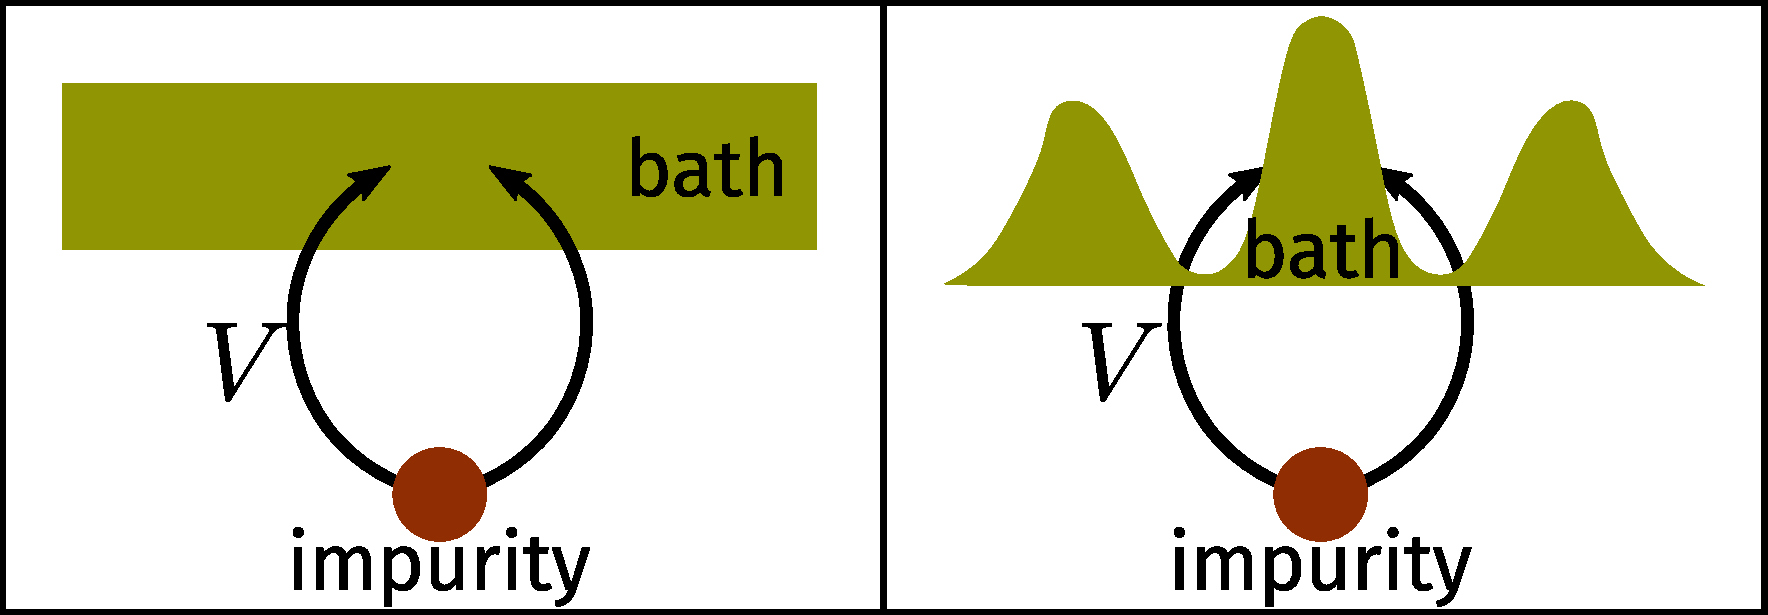
\includegraphics[width=0.5\textwidth]{../figures/dos_diff.pdf}
\caption{Various kinds of bath that an impurity can hybridise into. The left panel shows a non-interacting conduction band with a flat density of states. The right panel shows an interacting bath with an energy-dependent density of states. In the latter case, the impurity "feels" a reduced effective bandwidth defined by the width of the central peak.}
\end{figure}

\section{Philosophy of auxiliary model methods}
The present method is a realisation of the general method of using simpler systems called auxiliary models to study bulk systems~\cite{martin_2016}. In general, a full Hamiltonian can be separated into the Hamiltonians for a particular subsystem \(S\), the rest of the system \(R\), and the interactions between \(S\) and \(R\).
\begin{equation}\begin{aligned}
	\mathcal{H} = \mathcal{H}_S\ket{S}\bra{S} + \mathcal{H}_R \ket{R}\bra{R} + \mathcal{H}_{SR} \ket{S}\bra{R} + \mathcal{H}_{RS}\ket{S}\bra{R} = \begin{bmatrix} & \mathcal{H}_{R} && \mathcal{H}_{RS} & \\ & \mathcal{H}_{RS}^* && \mathcal{H}_{S} & \end{bmatrix}
\end{aligned}\end{equation}
where \(\ket{S}\) and \(\ket{R}\) actually represents sums over all basis kets of \(S\) and \(R\) respectively. As an example, we can split the Hubbard model Hamiltonian between a particular site \(i = p\) and the rest of the lattice as follows (fig.~\ref{cluster-bath}):
\begin{equation}\begin{aligned}
	H_\text{hubb} &= \overbrace{U^H\hat n_{p \uparrow} \hat n_{p \downarrow} - \mu^H \sum_\sigma \hat n_{p \sigma}}^{H_S} + \underbrace{U^H\sum_{i \neq p}\hat n_{i \uparrow} \hat n_{p \downarrow} - \mu^H \sum_{i \neq p, \sigma} \hat n_{i \sigma} -t^H\sum_{\sigma,\left<i,j \right>\atop{i \neq p \neq j}}\left(c^\dagger_{i\sigma} c_{j\sigma} + \text{h.c.}\right)}_{H_R}\\
		      & -\underbrace{t^H\sum_{\sigma,\atop{i \in \text{N.N. of }p}}\left(c^\dagger_{i\sigma} c_{p\sigma} + \text{h.c.}\right)}_{H_{SR} + H_{RS}}\\
\end{aligned}\end{equation}
The Greens function of the full Hamiltonian can also be split in a similar fashion:
\begin{equation}\begin{aligned}
	G(\omega) = \begin{bmatrix} G_S && G_{SR} \\ G_{RS} && G_R \end{bmatrix}
\end{aligned}\end{equation}
Each Greens function can be written in terms of the non-interacting counterpart and the self-energy through the Dyson equation: \(\Sigma_i = 1/G_{i,0} - 1/G_i\).

The subsystem \(S\) is usually taken to be the "cluster", and consequently, \(R\) represents the "bath".
The smaller system is typically chosen such that its eigenstates are known exactly.
Progress is then made by choosing a simpler version of \(H_R\) and a simpler form also for its coupling \(H_{RS}\) with the smaller system.
This combination of the cluster and the simpler bath is then called the \textit{auxiliary system}.
A typical auxiliary system for the Hubbard model would be the SIAM, where the impurity represents an arbitrary site \(p\) of the lattice, the bath represents the rest of the lattice sites and the hybridisation term between the impurity and the bath represents the coupling term \(H_{RS}\).
Such a construction is shown in fig.~\ref{cluster-bath}.
\begin{figure}[!htb]
	\centering
	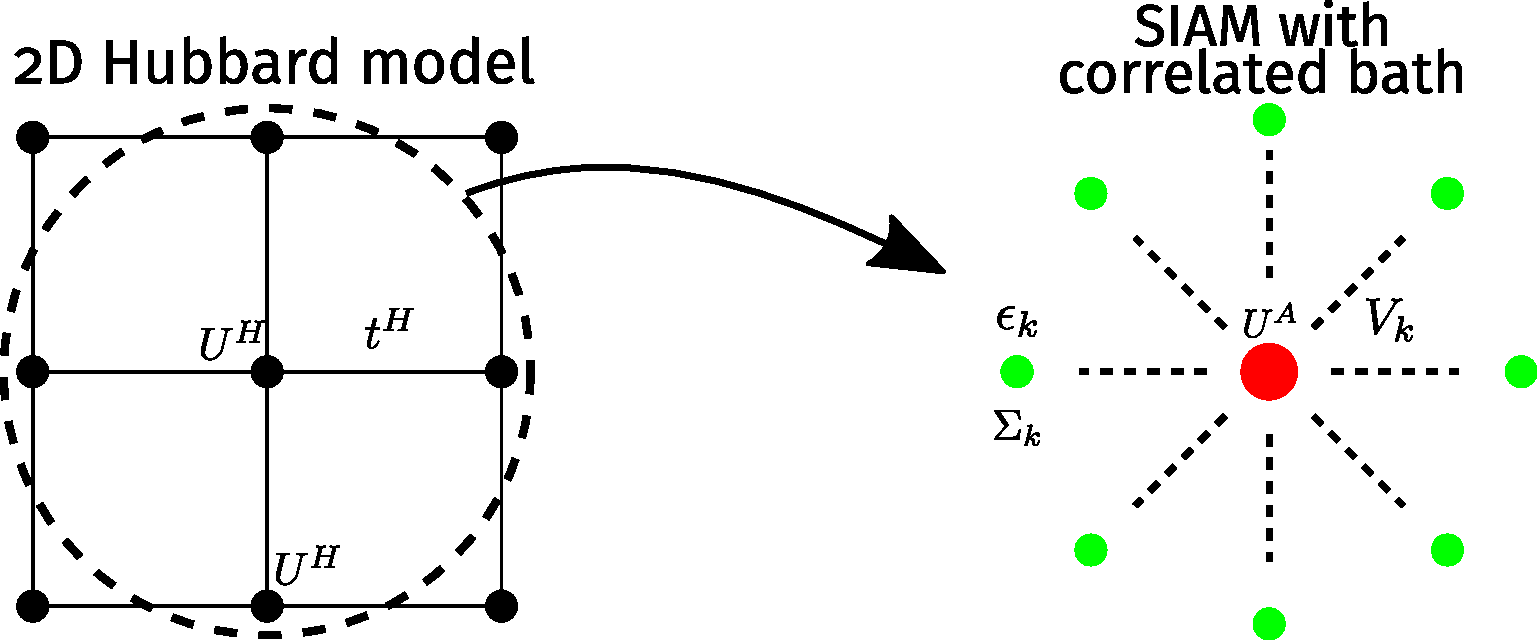
\includegraphics[width=0.8\textwidth]{../figures/cluster-bath.pdf}
	\caption{\textit{Left}: Full Hubbard model lattice with onsite repulsion $U^H$ on all sites and hopping between nearest neighbour sites with strength $t^H$. \textit{Right}: Extraction of the auxiliary (cluster+bath) system from the full lattice. The central site on left becomes the impurity site (red) on the right (with an onsite repulsion $\epsilon_d$), while the rest of the $N-1$ sites on the left form a conduction bath (green circles) (with dispersion $\epsilon_k$ and correlation modelled by the self-energy $\Sigma_k(\omega)$) that hybridizes with the impurity through the coupling $V$.}
	\label{cluster-bath}
\end{figure}
\textit{It should be noted that any reasonable choice of the cluster and bath would break the translational symmetry of the full model}. To allow computing quantities, one would need to make the bath (which is a much larger system) simpler than the cluster (which is a single site). This distinction breaks the translational symmetry of the Hubbard model. For eg., if one chooses eq.~\ref{clus_bath_siam} as the auxiliary system, then the fact that the impurity has an onsite correlation while the bath does not means we have broken the symmetry between the cluster and the bath.

\subsection*{Dynamical mean-field theory - an example of an auxiliary model approach}
Dynamical mean-field theory is an approximation scheme that use impurity models to obtain Greens functions of bulk systems of strong correlation~\cite{kotliar1996,kotliar1992}. The essential idea is to find the most suitable impurity model that replicates the full Hamiltonian. This is done through the following algorithm. Given a bulk Hamiltonian with on=site correlation \(U\) and a non-interacting \(k-\)space Greens function \(G_{k,0}\) for the bath:
\begin{itemize}
	\item[1.] We first create an impurity model with on-site correlation \(U\) and non-interacting impurity Greens function \(G_{i,0} = \sum_k G_{k,0}\).
		\[\mathcal{H}_\text{aux} = H_\text{imp}(U) -t \sum_\sigma \left(c^\dagger_{d\sigma}c_{0\sigma} + \text{h.c.}\right) + H_\text{bath}\left(t,G_{i,0}\right)\]

	\item[2.] This impurity model is solved using some method like numerical renormalisation group, and the self-energy \(\Sigma_\text{aux}\) of the impurity is obtained.

	\item[3.] The impurity self-energy is now {\it equated} with the bath momentum-space self-energy:
		\[\Sigma_{k}(\omega) = \Sigma_\text{aux}(\omega)\]
		Since the impurity is purely local, this is an approximation that involves replacing a non-local quantity by its purely local component: \(\Sigma_{k}(\omega) = \sum_{\vec r}e^{i \vec{k}\cdot\vec{r}}\Sigma_{\vec r}(\omega) \simeq \Sigma_{\vec r = 0}(\omega)\). This approximation is a result of the single-site nature of the cluster of the chosen auxiliary model - larger clusters with more impurities can generate non-local components. This local approximation becomes exact in the limit of large system dimension \(w\), because it can be shown that the non-local components of the self-energy scale as \(w^{-3/2}\).

	\item[4.] With this updated bath self-energy, we now create a new \(k-\)space Greens function for the bath:
		\[G_{i}(\omega) = \sum_k G_{k}(\omega) = \sum_k \frac{1}{\omega - H_\text{bath}(k) - \Sigma_k(\omega)} = \sum_k \frac{1}{\omega - H_\text{bath}(k) - \Sigma_\text{aux}(\omega)}\]
	This interacting Greens function is then used to obtain the updated non-interacting Greens function, using Dyson's equation:
	\[G_{i,0} = \frac{1}{1/G_{i} + \Sigma_\text{aux}}\]
	\item[5.] Repeat the algorithm from step 1 with the updated \(G_{i,0}\), until \(\Sigma_\text{aux}\) stops changing.
\end{itemize}
The stopping condition is the consistency relation that makes the bath and impurity self-energies equal.

\begin{figure}[!htb]
	\centering
	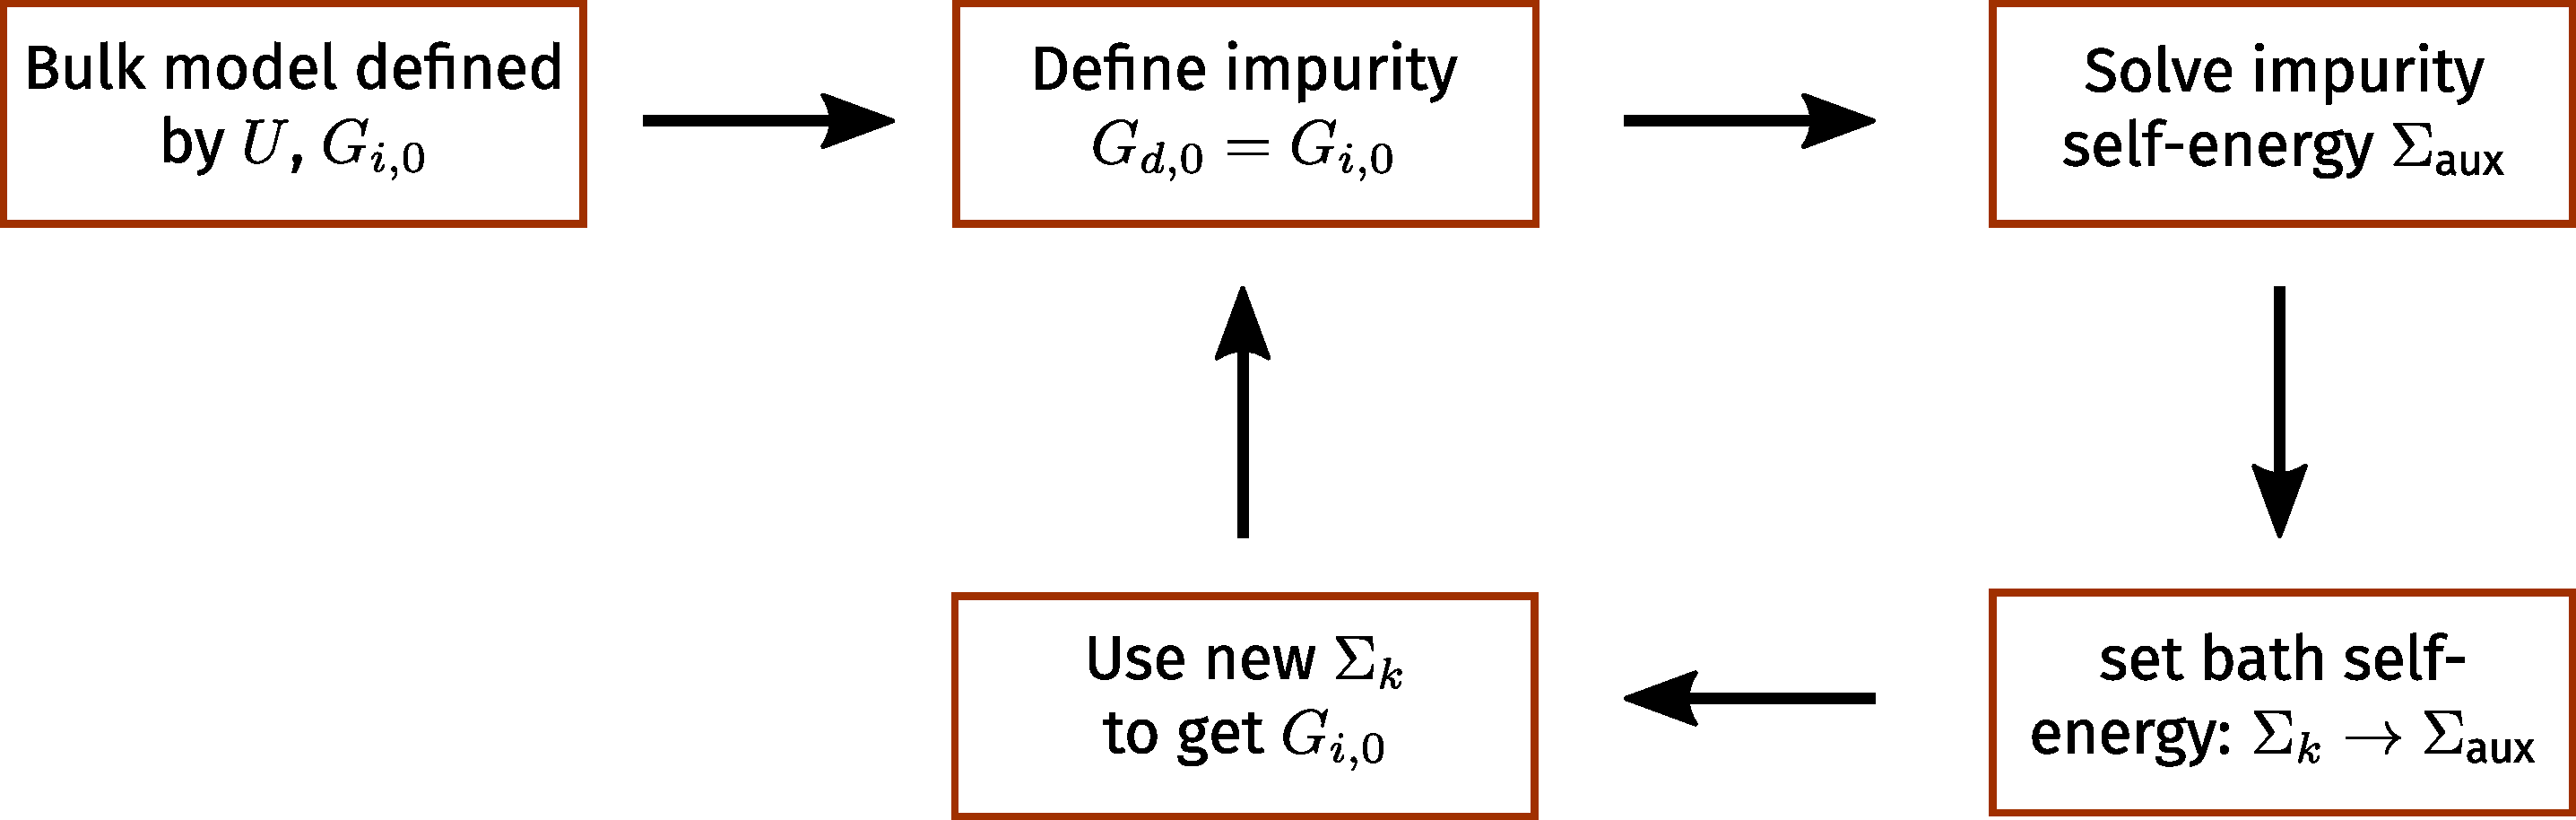
\includegraphics[width=0.8\textwidth]{../figures/dmft.pdf}
\end{figure}


\section{A "bottoms-up" approach to using auxiliary models}
As mentioned in the previous section, the question we are posing is the following: what is the simplest auxiliary model of impurity in a bath that can capture the metal-insulator transition in a Hubbard-like model of correlated electrons. We approach this problem in a constructionist/bottoms-up way: we first identity an appropriate quantum impurity model (fig.~\ref{cluster-bath}) that shows an impurity phase transition, and then create a bulk model out of this auxiliary model. The bulk model hence created will then show a metal-insulator transition. The impurity models are studied using the recently-developed unitary renormalisation group method~\cite{anirbanmott1,anirbanmott2,anirbanurg1,anirbanurg2,siddharthacpi,santanukagome}, and this analysis is shown in chapters~\ref{chap:urg1}~and~\ref{siam-attr-chap}. The leap to the bulk model is then made by applying lattice translation operators on the auxiliary model. This process is shown in chapter~\ref{chap:tile}. This process, referred to as tiling here, relates the auxiliary model Hamiltonian with that of the bulk, and hence allows connecting the Greens functions and other related quantities across dimensions. One nice outcome is that since the auxiliary model has multiple sites, there is a real-space off-diagonal component of the self-energy, and this leads to a \(k-\)dependence in the self-energy of the bulk, which is in contrast with the lack of \(k-\)dependence in single-site DMFT.  

In our approach, the auxiliary models can be chosen in various ways. The simplest choice is of course the single-impurity Anderson model of eq.~\ref{clus_bath_siam}:
\begin{equation}
\mathcal{H}_\text{SIAM} = \epsilon_d \hat n_d + U \hat n_{d \uparrow} \hat n_{d \downarrow} - t\sum_{\left<i,j \right>, \sigma}\left(c^\dagger_{i\sigma}c_{j\sigma} + \text{h.c.}\right) + V\sum_\sigma \left( c^\dagger_{d\sigma}c_{0\sigma} + \text{h.c.}\right) 
\end{equation}
This model does not show any impurity phase transition - the impurity is always screened~\cite{hrk_wilson_1980,wilson1975,bullaNRGreview}. Correlation can be introduced into the auxiliary model in two ways:
\begin{itemize}
	\item[1.] The impurity or the bath can be made to have additional interaction: 
\begin{gather}
\mathcal{H}_\text{aux} = H_\text{SIAM} + J \vec{S}_d\cdot\vec{s}_0\\
\mathcal{H}_\text{aux} = H_\text{SIAM} + J \vec{S}_d\cdot\vec{s}_0 - U_b \left(\hat n_{0 \uparrow} - \hat n_{0 \downarrow}\right)^2
\end{gather}
The first example has a spin-exchange interaction between the impurity site and the zeroth site, while the second example additionally has a correlation locally on the zeroth site.
\item[2.] The second method is to make the cluster itself more complicated. That is, one can introduce multiple impurity sites that are connected via the hopping:
\begin{equation}
\mathcal{H}_\text{aux} = -\frac{U}{2}\sum_{d_i}\left(\hat n_{d_i \uparrow} - \hat n_{d_i \downarrow}\right) ^2 + V\sum_{d_i}\sum_\sigma\left( c^\dagger_{d_i\sigma}c_{0\sigma} + \text{h.c.} \right) + \text{K.E.} - t\sum_{\sigma}\left(c^\dagger_{d_1\sigma}c_{d_2\sigma} + \text{h.c.}\right)
\end{equation}
	
\end{itemize}

\begin{figure}[!htb]
 	\centering
 	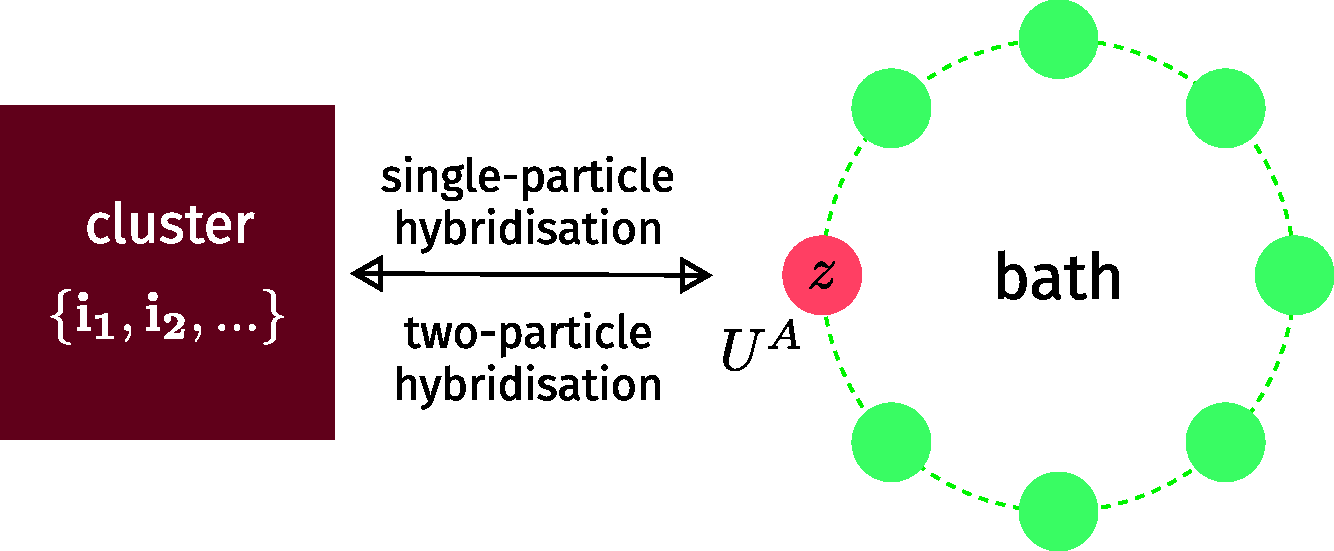
\includegraphics[width=0.6\textwidth]{../figures/gen_siam.pdf}
 	\caption{Cluster+bath construction of auxiliary model. It consists of a cluster (red square) hybridising with a bath (ring) by hopping into and out of the zeroth site (pink). The other sites (green) form the rest of the bath. Just the cluster and the zeroth site have onsite correlations.}
 \end{figure}
 The next step in the programme is to tile the real-space lattice with this cluster+bath Hamiltonian \(\tilde H\) to restore translational invariance (shown in a later section), and obtain a new bulk Hamiltonian for correlated electrons, $\tilde H = T\left[ \mathcal{H}_\text{aux} \right] T^{-1}$, where $T$ denotes the operator that performs the set of iterative real-space translations, and enables the cluster-bath (auxiliary model) Hamiltonian to span the target real-space lattice. Given a general auxiliary model Hamiltonian \(\mathcal{H}_\text{aux}\), the result of tiling can be written very generally as
 \begin{equation}\begin{aligned}
	 \tilde H = \sum_{\left\{i_1,i_2,...\right\}} \mathcal{H}_\text{aux}\left(\left\{i_1,i_2,...\right\}\right)
 \end{aligned}\end{equation}
where \(\left\{i_1,i_2,...\right\}\) represents the indices for the members of the cluster. To reiterate, what that means is that we have placed the cluster+bath system at all lattice point sets \(\left\{i_1,i_2,...\right\}\) to reconstruct a new model of correlated electrons. The answer to how closely $\tilde H$ approximates a target model of correlated electrons lies in (i) the choice of the cluster-bath construction of the auxiliary model, and (ii) the accuracy of the URG procedure on the auxiliary model. 

\chapter{From the auxiliary model to the bulk - single site approach}
\label{chap:tile}

\section{Creating \(N-\)site Hubbard Hamiltonian from Anderson impurity embedded in an interacting bath}

Previously, we have worked out the grounstate phases of a single-impurity model with an interacting bath:
\begin{equation}\begin{aligned}
	\label{siam_attr}
	\mathcal{H}_\text{aux} = \sum_{k\sigma}\epsilon_k \tau_{k\sigma} - \frac{U}{2}\left(\hat n_{d \uparrow} - \hat n_{d \downarrow} \right) ^2 + \sum_{k\sigma} \left(V_{k} c^\dagger_{k\sigma} c_{d\sigma} + h.c.\right) +J \vec{S_d}\cdot\vec{s} - U_b\left(\hat n_{0 \uparrow} - \hat n_{0 \downarrow}\right)^2 
\end{aligned}\end{equation}
 
We will use this as the auxiliary model to study the Hubbard model. We do this by first recreating the Hubbard model upon tiling the lattice with instances of this auxiliary model Hamiltonian. Note that the impurity level is explicitly at half-filling, because the correlation term \(\left( \hat n_{d \uparrow} - \hat n_{d \downarrow} \right) ^2\) is symmetric under a particle-hole transformation \(\hat n_{d\sigma} \to 1 - \hat n_{d\sigma}\). Moreover, the conduction bath is also at half-filling, because we have set the chemical potential \(\mu\) to zero. These two ensure that the bulk model is also at half-filling. At the end of this section, we will also mention how the tiling works out in the presence of a non-zero filling.

To begin this procedure, we first create the unit of tiling - this is done by identifying the impurity as a particular site \(i\) of the lattice, and the bath coupled to the impurity as the set of remaining \(N-1\) sites in the lattice. We will also identity the zeroth site of the SIAM lattice as one of the nearest neighbours \(j\) of \(i\):
\begin{equation}\begin{aligned}
	\mathcal{H}_\text{aux}(i,j) = -2t\sum_{<m,n>,\sigma}^{m \neq i \neq n} \left(c^\dagger_{m\sigma}c_{n\sigma} + \text{h.c.}\right) - \frac{U}{2}\left( \hat n_{i \uparrow} - \hat n_{i \downarrow} \right) ^2 + V \sum_{\sigma} \left(c^\dagger_{j\sigma} c_{i\sigma} + h.c.\right) +J \vec{S_i}\cdot\vec{S}_j - U_b\left(\hat n_{j \uparrow} - \hat n_{j \downarrow}\right)^2 
\end{aligned}\end{equation}
The tight-binding term sums over all nearest pairs \((m,n)\) that do not involve the site \(i\).
In general \(i\) will have \(w\) nearest neighbours for a lattice with coordination number \(w\). The total local Hamiltonian for the site \(i\) is obtained by averaging over the Hamiltonians \(\mathcal{H}_\text{aux}(i,j)\) for all nearest neighbours \(j\) of \(i\):
\begin{equation}\begin{aligned}
	\mathcal{H}_\text{aux}(i) &= \frac{1}{w}\sum_{j \in \text{NN of i}} \mathcal{H}_\text{aux}(i,j) = - \frac{U}{2}\left( \hat n_{i \uparrow} - \hat n_{i \downarrow} \right)^2 + \frac{1}{w}\sum_{j \in \text{NN of i}}\left[-2t\sum_{<m,n>,\sigma}^{m \neq i \neq n}\left(c^\dagger_{m\sigma}c_{n\sigma} + \text{h.c.}\right) + V \sum_{\sigma} \left(c^\dagger_{j\sigma} c_{i\sigma} + h.c.\right)  \right.\\
				  &\left. +J \vec{S_i}\cdot\vec{S}_j - U_b\left(\hat n_{j \uparrow} - \hat n_{j \downarrow}\right)^2\right]\\
				  &= - \frac{U}{2}\left( \hat n_{i \uparrow} - \hat n_{i \downarrow} \right)^2 -2t\sum_{<m,n>,\sigma}^{m \neq i \neq n}\left(c^\dagger_{m\sigma}c_{n\sigma} + \text{h.c.}\right) +  \frac{1}{w}\sum_{j \in \text{NN of i}}\left[V \sum_{\sigma} \left(c^\dagger_{j\sigma} c_{i\sigma} + h.c.\right) +J \vec{S_i}\cdot\vec{S}_j \right.\\
				  &\left.- U_b\left(\hat n_{j \uparrow} - \hat n_{j \downarrow}\right)^2\right]
\end{aligned}\end{equation}
Once we have this local Hamiltonian for a particular site, we translate this over all sites \(i\):
\begin{equation}\begin{aligned}
	\mathcal{H}_\text{full} =& \sum_i \mathcal{H}_\text{aux}(i) = \sum_i\left[- \frac{U}{2}\left( \hat n_{i \uparrow} - \hat n_{i \downarrow} \right)^2 -2t\sum_{<m,n>,\sigma}^{m \neq i \neq n}\left(c^\dagger_{m\sigma}c_{n\sigma} + \text{h.c.}\right) +  \frac{1}{w}\sum_{j \in \text{NN of i}}\left[V \sum_{\sigma} \left(c^\dagger_{j\sigma} c_{i\sigma} + h.c.\right) \right.\right.\\
				  &\left.\left. + J \vec{S_i}\cdot\vec{S}_j - U_b\left(\hat n_{j \uparrow} - \hat n_{j \downarrow}\right)^2\right]\right]\\
	=& -\left(\frac{U}{2} + U_b\right) \sum_i \left( \hat n_{i \uparrow} - \hat n_{i \downarrow} \right)^2 + \sum_i\left[-2t\sum_{<m,n>,\sigma}^{m \neq i \neq n}\left(c^\dagger_{m\sigma}c_{n\sigma} + \text{h.c.}\right) +  \frac{1}{w}\sum_{j \in \text{NN of i}}\left[V \sum_{\sigma} \left(c^\dagger_{j\sigma} c_{i\sigma} + h.c.\right) \right.\right.\\
				  &\left.\left. + J \vec{S_i}\cdot\vec{S}_j\right]\right]
\end{aligned}\end{equation}
In the entire tight-binding term \(\sum_i\sum_{<m,n>,\sigma}^{m \neq i \neq n}\), each pair will appear \(N-2\) times, because that is the total number of sites that do not involve either \(m\) or \(n\).
\begin{equation}\begin{aligned}
	\mathcal{H}_\text{full} =& -\left(\frac{U}{2} + U_b\right) \sum_i \left( \hat n_{i \uparrow} - \hat n_{i \downarrow} \right)^2 - 2t\left(N-2\right)\sum_{<m,n>,\sigma}\left(c^\dagger_{m\sigma}c_{n\sigma} + \text{h.c.}\right) + \frac{2}{w}\sum_{<i,j>}\left[\sum_\sigma V \left(c^\dagger_{j\sigma} c_{i\sigma} + h.c.\right) \right.\\
				  &+ \left. J \vec{S_i}\cdot\vec{S}_j\right]\\
				  &=-\left(\frac{U}{2} + U_b\right) \sum_i \left(\hat n_{i \uparrow} - \hat n_{i \downarrow} \right)^2 - \left(2t (N-2) - \frac{2V}{w}\right) \sum_{<m,n>,\sigma}\left(c^\dagger_{m\sigma}c_{n\sigma} + \text{h.c.}\right) + \frac{2J}{w} \sum_{<i,j>} \vec{S_i}\cdot\vec{S}_j 
\end{aligned}\end{equation}
We end up with a Hubbard-Heisenberg model:
\begin{equation}\begin{aligned}
	\mathcal{H}_{H-H} = -\sum_{i} U_\text{H-H} \left(\hat n_{i \uparrow} - \hat n_{i \downarrow} \right)^2 - t_\text{H-H}\sum_{<i,j>,\sigma}\left(c^\dagger_{i\sigma}c_{j\sigma} + \text{h.c.}\right) + J_\text{H-H}\sum_{<i,j>} \vec{S}_i\cdot\vec{S}_j
\end{aligned}\end{equation}
The mapping between the parameters is
\begin{equation}\begin{aligned}
	\label{map_aux_bulk}
	t_{H-H} = \left(2t (N-2) - \frac{2V}{w}\right),~ ~ U_{H-H} = \left(\frac{U}{2} + U_b\right), ~ ~ J_{H-H} = \frac{2J}{w}
\end{aligned}\end{equation}
The conclusion is that we can tile Anderson models with interacting baths into a Hubbard-Heisenberg model:
\begin{equation}\begin{aligned}
	\label{siam_to_hubb}
	\sum_i \mathcal{H}_\text{aux}(i) = \mathcal{H}_{H-H}
\end{aligned}\end{equation}

As mentioned before, no chemical potential \(\mu\) is generated becuase the auxiliary model was at half-filling, both in the impurity as well as in the bath. We can change the chemical potential by introducing two terms:
\begin{equation}\begin{aligned}
	\eta \sum_\sigma\left(n_{d\sigma} - \frac{1}{2}\right), \mu \sum_{i,\sigma}\left(\hat n_{i\sigma} - \frac{1}{2}\right)
\end{aligned}\end{equation}
The first term is the particle-hole asymmetry term, and tuning that term moves the impurity away from half-filling. The second term is the usual chemical potential in the bath. Introducing these terms in the auxiliary model changes the bulk model into:
\begin{equation}\begin{aligned}
	\mathcal{H}_{H-H} = -\sum_{i} U_\text{H-H} \left(\hat n_{i \uparrow} - \hat n_{i \downarrow} \right)^2 - t_\text{H-H}\sum_{<i,j>,\sigma}\left(c^\dagger_{i\sigma}c_{j\sigma} + \text{h.c.}\right) + J_\text{H-H}\sum_{<i,j>} \vec{S}_i\cdot\vec{S}_j + \mu_\text{H-H}\sum_{i\sigma}\left(\hat n_{i\sigma} - \frac{1}{2}\right) 
\end{aligned}\end{equation}
The only change is the generation of the last term. The mappings between the existing parameters and their auxiliary model counterparts remain the same, while \(\mu_\text{H-H}\) is given by
\begin{equation}\begin{aligned}
	\mu_\text{H-H} = \eta + \left(N-1\right) \mu
\end{aligned}\end{equation}
In the discussion henceforth, we will assume all the models are at half-filling. We will come back to the doped case at a later point in time.

\section{Nature of the wavefunctions}
In the tight-binding approach to lattice problems, the full Hamiltonian is described by adding the localised Hamiltonians at each site, and the full wavefunction \(\Psi\) is then obtained by constructing liner combinations of the eigenstates \(\psi_i\) of the local Hamiltonians such that \(\Psi\) satisfies Bloch's theorem: \(\Psi_{\vec k}(\vec r) = \sum_i e^{i \vec{k}\cdot\vec{R}_i} \psi_i(\vec r - \vec R_i)\). Bloch's theorem ensures that eigenstates satisfy the following relation under a translation operation \(T(\vec R)\) by some lattice distance \(\vec R = \sum_i n_i \vec a_i\):
\begin{equation}\begin{aligned}
T(\vec R)\Psi_{\vec k}\left(\vec r\right) = \Psi_{\vec k}(\vec r + \vec R) = \sum_i e^{i \vec{k}\cdot\vec{R}_i} \psi_i(\vec r + \vec R - \vec R_i) = e^{i \vec{k}\cdot\vec{R}}\sum_i e^{i \vec{k}\cdot\left(\vec{R}_i - \vec R\right)} \psi_i(\vec r - (\vec R_i - \vec R)) = e^{\vec{k}\cdot\vec{R}}\Psi(\vec r)
\end{aligned}\end{equation}
At the end, we used the fact that \(\vec r_i - \vec R\) is just another lattice vector \(\vec R_j\). Note that the translation operator has been defined as an operation that simply advances the argument of the wavefunction from \(\vec r\) to \(\vec r + \vec R\). An equivalent definition can be given in terms of their action on position eigenkets: \(T(\vec R)\ket{\vec r} = \ket{\vec r - \vec R}\). These translation operators share eigenstates with the momentum operator:
\begin{equation}\begin{aligned}
	T\left( \vec R \right) \ket{\vec k} = \sum_{\vec r_i} e^{i \vec{k}\cdot\vec{r}_i}T\left( \vec R \right)\ket{\vec r_i} = e^{i \vec{k}\cdot\vec{R}}\sum_{\vec r_i} e^{i \vec{k}\cdot\left(\vec{r}_i - \vec R\right)}\ket{\vec r_i - \vec R} = e^{i \vec{k}\cdot\vec{R}} \ket{\vec k}
\end{aligned}\end{equation}


The bulk Hamiltonian obtained in eq.~\ref{siam_to_hubb},
\begin{equation}\begin{aligned}
	H_\text{H-H}\left(\left\{\vec r_k\right\}\right) = \sum_{\vec R_i} \mathcal{H}_\text{aux,i}\left(\left\{\vec r_k - \vec R_i\right\}\right) \equiv \sum_{\vec R_i} \mathcal{H}_\text{aux}\left(\vec R_i\right)~,
\end{aligned}\end{equation}
also enjoys a Bloch's theorem. This is because the tiling procedure restores the translation symmetry of the lattice:
\begin{equation}\begin{aligned}
	H_\text{H-H}\left(\left\{\vec r_k + \vec R\right\}\right) =  \sum_{\vec R_i}\mathcal{H}_\text{aux,i}\left(\left\{\vec r_k - \vec R_i + \vec R\right\}\right) = \sum_{\vec R_i} \mathcal{H}_{\text{aux},\tilde i}\left(\left\{\vec r_k - \vec R\right\}\right) = H_\text{H-H}(\left\{\vec r_k\right\})
\end{aligned}\end{equation}
There we used the fact that \(\vec r_k + \vec R\) simply translates the auxiliary model defined by the coordinate \(i\) to a new auxiliary model at the modified coordinate \(\tilde i: \vec R_i^\prime = \vec R_i + \vec R\). Since this transformation from one auxiliary model to another simply shuffles the group of all auxiliary models, the sum over the group remains the sum, and we recover the same bulk model.

We can use the auxiliary model zero-bandwidth wavefunctions 
\begin{equation}\begin{aligned}
\psi^n_\text{aux}\left(\vec r_d - \vec R_i, \vec r_0 - \left(\vec R_i + \vec a\right)  \right) \equiv \psi^n_\text{aux}\left(\vec R_i, \vec a\right)
\end{aligned}\end{equation}
with the impurity position \(\vec R_i\) and zeroth site position \(\vec R_i + \vec a\), to construct eigenstates of the bulk Hamiltonian. \(\vec R_i\) is a lattice vector, while \(\vec a\) is one of the \(w\) vectors that connect a lattice site with its nearest neighbours. This two site wavefunction can be obtained by first studying the full auxiliary model \(\mathcal{H}_\text{aux}\) under a renormalisation group, obtaining a fixed-point Hamiltonian in the IR, obtaining the IR eigenstate and then tracing out all lattice sites except the impurity and the zeroth site from this eigenstate. \(n=0\) is the ground state of the auxiliary model, and higher values denote the excited states.

The following un-normalised combination of the auxiliary model eigenstates satisfies Bloch's theorem~\cite{stoyanova}:
\begin{equation}\begin{aligned}
	\ket{\Psi^n_{\vec k}} = \frac{1}{w \sqrt N}\sum_{\vec R_i, \vec a} e^{i \vec{k}\cdot\vec{R}_i} \psi^n_\text{aux}\left(\vec R_i, \vec a\right)
\end{aligned}\end{equation}
where \(N\) is the total number of lattice sites. The interpretation is that the set of \(n=0\) states form the lowest band in the spectrum of the lattice. Higher values of \(n\) produce the more energetic bands. The ground state is obtained by setting \(\vec k\) and \(n\) to 0: \(\ket{\Psi_{\vec k=0}^{n=0}} \equiv \ket{\Psi_\text{gs}}\). We will actually work only in the lowest band \(n=0\), so we will drop the band index from now on and keep in mind that only the auxiliary model ground states appear in the formulation:
\begin{equation}\begin{aligned}
	\label{bloch-states}
	\ket{\Psi_{\vec k}} = \frac{1}{\lambda_{\ket{\vec k}} w N}\sum_{\vec R_i, \vec a} e^{i \vec{k}\cdot\vec{R}_i} \psi_\text{aux}\left(\vec R_i, \vec a\right)~,
\end{aligned}\end{equation}
where \(\lambda_{\ket{\vec k}}\) is a normalisation factor. To determine this, we compute the norm of the trail eigenstates:
\begin{equation}\begin{aligned}
	\braket{\Psi_{\vec k} | \Psi_{\vec k}} &= \frac{1}{w^2 \lambda_{\vec k}^2 N^2}\sum_{\vec R, \vec R^\prime, a, a^\prime}e^{i \vec{k}\cdot(\vec R - \vec R^\prime)}\braket{\psi_\text{aux}(\vec R^\prime, \vec a^\prime) | \psi_\text{aux}(\vec R, \vec a)} = \frac{1}{\lambda_{\vec k}^2 N^2}\sum_{\vec R, \vec R^\prime, }e^{i \vec{k}\cdot(\vec R - \vec R^\prime)}\braket{\psi_\text{aux}(\vec R^\prime) | \psi_\text{aux}(\vec R)}\\
					       &=\frac{1}{\lambda_{\vec k}^2 N^2}\sum_{\vec R, \vec R^\prime}e^{i \vec{k}\cdot(\vec R - \vec R^\prime)}\braket{\psi_\text{aux}(\vec R_0) | T^\dagger(\vec R - \vec R^\prime) | \psi_\text{aux}(\vec R_0)} = \frac{1}{\lambda_{\vec k}^2 N^2}\sum_{\vec R, \vec R^\prime, q}e^{i \vec{k}\cdot(\vec R - \vec R^\prime)}\braket{\psi_\text{aux}(\vec R_0) | T^\dagger(\vec R - \vec R^\prime) \ket{\vec q}\bra{\vec q} \psi_\text{aux}(\vec R_0)}\\
					       &= \frac{1}{\lambda_{\vec k}^2 N^2}\sum_{\vec R, \vec R^\prime, q}e^{i (\vec{k} - \vec q)\cdot(\vec R - \vec R^\prime)}\braket{\psi_\text{aux}(\vec R_0) \ket{\vec q}\bra{\vec q} \psi_\text{aux}(\vec R_0)} = \frac{1}{\lambda_{\vec k}^2 N^2}\sum_{q} N^2 \delta_{\vec{k},\vec q}|\braket{\psi_\text{aux}(\vec R_0) | \vec q}|^2\\
\end{aligned}\end{equation}
By requiring this norm to be unity, we obtain \(\lambda_{\vec k}^2 = |\braket{\psi_\text{aux}(\vec R_0) | \vec k}|^2\). In the above exercise, we defined a state \(\ket{\psi_\text{aux}(\vec R)} = (1/w)\sum_{\vec a}\ket{\psi_\text{aux}(\vec R, \vec a)}\) by averaging over the neasest neighbours of \(\vec R\), and inserted the total momentum basis \(1 = \sum_{\vec q}\ket{\vec q}\bra{\vec q}\) to resolve the translation operators. \(\vec R_0\) is any particular lattice site which we define as the origin of the lattice. Because of the symmetry of the lattice, the inner product in the definition of \(\lambda\) will be the same irrespective of which \(\vec a\) we choose among the \(w\) choices.

It is easy to verify that \(\Psi_{\vec k}\left(\left\{ \vec r_k \right\}  \right) \) transforms like Bloch functions under translation by a displacement \(\vec R\):
\begin{equation}\begin{aligned}
	\Psi_{\vec k}\left(\left\{\vec r_k + \vec R\right\} \right) = \frac{1}{\lambda_{\ket{\vec k}} w N}\sum_{\vec R_i,\vec a} e^{i \vec{k}\cdot\vec{R}_i} \psi_\text{aux}\left(\vec R_i - \vec R, \vec a\right) = \frac{1}{\lambda_{\ket{\vec k}} w N}\sum_{\vec R_j, \vec a} e^{i \vec{k}\cdot\left(\vec{R}_j + \vec R\right)} \psi_\text{aux}\left(\vec R_j, \vec a\right) = e^{i \vec{k}\cdot\vec{R}} \Psi_{\vec k}\left(\left\{ \vec r_k \right\} \right)
\end{aligned}\end{equation}
In the last equation, we transformed \(\vec R_i \to \vec R_j = \vec R_i - \vec R\). Note that the argument \(\vec a\) does not change under a translation of the system, because that vector always represents the difference between the impurity lattice position and its nearest neighbours, irrespective of the absolute position of the impurity.

The wavefunction can be even brought into the familiar Bloch function form:
\begin{equation}\begin{aligned}
	\Psi^n_{\vec k}\left(\left\{\vec r_k\right\}\right) = \sum_{\vec R_i, \vec a} \frac{e^{i \vec{k}\cdot\vec{R}_i}}{\lambda_{\ket{\vec k}} w N} \psi_\text{aux}\left(\left\{ \vec r_d - \vec R_i, \vec r_0 - \vec R_i - \vec a \right\} \right) = \frac{e^{i \vec{k}\cdot\frac{1}{N}\sum_k \vec{r}_k}}{\lambda_{\ket{\vec k}} w N}\sum_{\vec R_i, \vec a} e^{-i \vec{k}\cdot\left(\frac{1}{N}\sum_k\vec r_k - \vec{R}_i\right)} \psi_\text{aux}\left(\left\{ \vec r_d - \vec R_i, \vec r_0 - \vec R_i - \vec a \right\} \right) \\
	= e^{i \vec{k}\cdot\vec{r}_\text{COM}} \eta_{\vec k}\left(\left\{\vec r_k\right\}\right)
\end{aligned}\end{equation}
where \(\vec r_\text{COM} = \frac{1}{N}\sum_k \vec r_k\) is the center-of-mass coordinate and \(\eta_{\vec k}\left(\left\{\vec r_k\right\}\right) = \frac{1}{\lambda_{\ket{\vec k}} w N}\sum_{\vec R_i} e^{-i \vec{k}\cdot\left(\frac{1}{N}\sum_k\vec r_k - \vec{R}_i\right)} \psi^n_\text{aux}\left(\left\{\vec r_k - \vec R_i\right\}\right)\) is the translation symmetric function. This form of the eigenstate allows the interpretation that tuning the Bloch momentum \(\vec k\) corresponds to a translation of the center of mass of the system (or in this case, of the auxiliary models that comprise the system).

It is straightforward to show that these states form an orthonormal basis. We start by writing down the inner product of two distinct such states:
\begin{equation}\begin{aligned}
	\braket{\Psi_{\vec k^\prime} | \Psi_{\vec k}} 
	&= \frac{1}{\lambda_{\ket{\vec k^\prime}}^* \lambda_{\ket{\vec k}} w^2 N^2}\sum_{\vec R_i, \vec R_j, \vec a, \vec a^\prime} e^{i \left(\vec{k}\cdot\vec{R}_i - \vec{k}^\prime\cdot\vec{R}_j\right) } \braket{\psi_\text{aux}\left( \vec R_j, \vec a^\prime \right) | \psi_\text{aux}\left( \vec R_i, \vec a \right)} \\
	&= \frac{1}{\lambda_{\ket{\vec k^\prime}}^* \lambda_{\ket{\vec k}} w^2 N^2}\sum_{\vec R_i, \vec R_j, \vec a, \vec a^\prime} e^{i \left(\vec{k}\cdot\vec{R}_i - \vec{k}^\prime\cdot\vec{R}_j\right) } \braket{\psi_\text{aux}\left( \vec R_0, \vec a^\prime \right) T^\dagger\left( \vec R_0 - \vec R_j \right) T\left( \vec R_0 - \vec R_i \right) | \psi_\text{aux}\left( \vec R_0, \vec a \right)}\\
\end{aligned}\end{equation}
At this point, we insert a complete basis of momentum eigenkets \(1 = \sum_{\vec q}\ket{\vec q}\bra{\vec q}\) to resolve the translation operators:
\begin{equation}\begin{aligned}
	\braket{\Psi_{\vec k^\prime} | \Psi_{\vec k}} &= \frac{1}{\lambda_{\ket{\vec k^\prime}}^* \lambda_{\ket{\vec k}} w^2 N^2}\sum_{\vec R_i, \vec R_j, \vec a, \vec a^\prime, \vec q} e^{i \left(\vec{k}\cdot\vec{R}_i - \vec{k}^\prime\cdot\vec{R}_j\right) } \braket{\psi_\text{aux}\left( \vec R_0, \vec a^\prime \right) T\left( \vec R_j - \vec R_i \right) \ket{\vec q}\bra{\vec q} \psi_\text{aux}\left( \vec R_0, \vec a \right)}\\
						      &= \frac{1}{\lambda_{\ket{\vec k^\prime}}^* \lambda_{\ket{\vec k}} w^2 N^2}\sum_{\vec R_i, \vec R_j, \vec a, \vec a^\prime, \vec q} e^{i \left(\vec{k}\cdot\vec{R}_i - \vec{k}^\prime\cdot\vec{R}_j\right) } \braket{\psi_\text{aux}\left( \vec R_0, \vec a^\prime \right) e^{i \vec q \cdot \left( \vec R_j - \vec R_i \right)} \ket{\vec q}\bra{\vec q} \psi_\text{aux}\left( \vec R_0, \vec a \right)} \\
						      &= \frac{1}{|\lambda_{\ket{\vec k}}|^2 w^2} \delta_{\vec k, \vec k^\prime}\sum_{\vec a, \vec a^\prime}\braket{\psi_\text{aux}\left( \vec R_0, \vec a^\prime \right) \ket{\vec k}\bra{\vec k} \psi_\text{aux}\left( \vec R_0, \vec a \right)}\\
\end{aligned}\end{equation}
At the last step, we used the summation form of the Kronecker delta function: \(\sum_{\vec R_i}e^{i \vec R_i \left( \vec k - \vec q \right) }\sum_{\vec R_j}e^{i \vec R_j \left( \vec q - \vec k^\prime \right) } = N \delta_{\vec k,\vec q}N \delta_{\vec k^\prime,\vec q}\). The final remaining step is to identify that the inner products inside the summation are actually independent of the direction \(\vec a, \vec a^\prime\) of the connecting vector, and both are equal to the normalisation factor \(\lambda_{\ket{\vec k}}\):
\begin{equation}\begin{aligned}
	\braket{\Psi_{\vec k^\prime} | \Psi_{\vec k}} = \frac{1}{|\lambda_{\ket{\vec k}}|^2 w^2 } \delta_{\vec k, \vec k^\prime}\sum_{\vec a,\vec a^\prime} |\lambda_{\ket{\vec k}}|^2 = \frac{1}{|\lambda_{\ket{\vec k}}|^2 w^2 } \delta_{\vec k, \vec k^\prime}w^2 |\lambda_{\ket{\vec k}}|^2 = \delta_{\vec k, \vec k^\prime}
\end{aligned}\end{equation}
This concludes the proof of orthonormality.

To demonstrate that these are indeed eigenstates of the bulk Hamiltonian, we will calculate the matrix elements of the full Hamiltonian between these states:
\begin{equation}\begin{aligned}
	&\bra{\Psi_{\vec k^\prime}}H_\text{H-H} \ket{\Psi_{\vec k}} = \frac{1}{\lambda^*_{\ket{\vec k^\prime}} \lambda_{\ket{\vec k}} w^2 N^2}\sum_{\vec R_i, \vec R_j, \vec R_k, \vec a, \vec a^\prime}e^{i\left(\vec{k}\cdot\vec{R}_i - \vec{k}^\prime\cdot\vec{R}_j\right)} \bra{\psi_\text{aux}\left(\vec R_j, \vec a^\prime\right)} H_\text{aux}\left(\vec R_k\right) \ket{\psi_\text{aux}\left(\vec R_i, \vec a\right)}\\
	&= \frac{1}{\lambda^*_{\ket{\vec k^\prime}} \lambda_{\ket{\vec k}} w^2 N^2}\sum_{\vec R_i, \vec R_j, \vec R_k, \vec a, \vec a^\prime}e^{i\left(\vec{k}\cdot\vec{R}_i - \vec{k}^\prime\cdot\vec{R}_j\right)} \bra{\psi_\text{aux}\left(\vec R_0, \vec a^\prime\right)} T^\dagger_{\vec R_0 - \vec R_j} T_{\vec R_0 - \vec R_k} H_\text{aux}\left(\vec R_0\right) T^\dagger_{\vec R_0 - \vec R_k} T_{\vec R_0 - \vec R_i} \ket{\psi_\text{aux}\left(\vec R_0, \vec a\right)}\\
	&= \frac{1}{\lambda^*_{\ket{\vec k^\prime}} \lambda_{\ket{\vec k}} w^2 N^2}\sum_{\vec R_i, \vec R_j, \vec R_k, \vec a, \vec a^\prime}e^{i\left(\vec{k}\cdot\vec{R}_i - \vec{k}^\prime\cdot\vec{R}_j\right)} \bra{\psi_\text{aux}\left(\vec R_0, \vec a^\prime\right)} T^\dagger_{\vec R_k - \vec R_j} H_\text{aux}\left(\vec R_0\right) T_{\vec R_k - \vec R_i} \ket{\psi_\text{aux}\left(\vec R_0, \vec a\right)}
\end{aligned}\end{equation}
To resolve the translation operators, we will now insert the momentum eigenstates \(\ket{\vec k}\) of the full model: \(1 = \sum_{\vec q}\ket{\vec q}\bra{\vec q}\) in between the operators.
\begin{equation}\begin{aligned}
	\bra{\Psi_{\vec k^\prime}}H_\text{H-H} \ket{\Psi_{\vec k}} &= \sum_{\vec R_i, \vec R_j, \vec R_k, \atop{\vec a, \vec a^\prime, \vec q, \vec q^\prime}}\frac{e^{i\left(\vec{k}\cdot\vec{R}_i - \vec{k}^\prime\cdot\vec{R}_j\right)}}{\lambda^*_{\ket{\vec k^\prime}} \lambda_{\ket{\vec k}} w^2 N^2} \braket{\psi_\text{aux}\left(\vec R_0, \vec a^\prime\right)| \vec q^\prime}\bra{\vec q^\prime} T^\dagger_{\vec R_k - \vec R_j} H_\text{aux}\left(\vec R_0\right) T_{\vec R_k - \vec R_i}  \ket{\vec q}\braket{\vec q | \psi_\text{aux}\left(\vec R_0, \vec a\right)}\\
								   &= \sum_{\vec R_i, \vec R_j, \vec R_k, \atop{\vec a, \vec a^\prime, \vec q, \vec q^\prime}}\frac{e^{i\left(\vec{k}\cdot\vec{R}_i - \vec{k}^\prime\cdot\vec{R}_j\right)}}{\lambda^*_{\ket{\vec k^\prime}} \lambda_{\ket{\vec k}} w^2 N^2} \braket{\psi_\text{aux}\left(\vec R_0, \vec a^\prime\right)| \vec q^\prime} e^{-i \vec q^\prime \cdot \left(\vec R_k - \vec R_j\right) } e^{i \vec q \cdot \left(\vec R_k - \vec R_i\right)} \braket{\vec q^\prime | H_\text{aux}\left(\vec R_0\right) | \vec q}  \braket{\vec q | \psi_\text{aux}\left(\vec R_0, \vec a\right)}\\
								   &= \frac{N}{\lambda^*_{\ket{\vec k^\prime}} \lambda_{\ket{\vec k}} w^2}\sum_{\vec a, \vec a^\prime, \vec q, \vec q^\prime} \delta_{\vec k, \vec q} \delta_{\vec q,\vec q^\prime} \delta_{\vec q^\prime,\vec k} \braket{\psi_\text{aux}\left(\vec R_0, \vec a^\prime\right)| \vec q^\prime} \braket{\vec q^\prime | H_\text{aux}\left(\vec R_0\right) | \vec q}  \braket{\vec q | \psi_\text{aux}\left(\vec R_0, \vec a\right)}\\
								   &= \frac{N}{|\lambda_{\ket{\vec k}}|^2 w^2}\delta_{kk^\prime}\sum_{\vec a, \vec a^\prime} \braket{\psi_\text{aux}\left(\vec R_0, \vec a^\prime\right)| \vec k} \braket{\vec k | H_\text{aux}\left(\vec R_0\right) | \vec k}  \braket{\vec k | \psi_\text{aux}\left(\vec R_0, \vec a\right)}\\
								   &= \frac{N}{|\lambda_{\ket{\vec k}}|^2 w^2}\delta_{kk^\prime}\braket{\vec k | H_\text{aux}\left(\vec R_0\right) | \vec k} \underbrace{\sum_{\vec a, \vec a^\prime} \braket{\psi_\text{aux}\left(\vec R_0, \vec a^\prime\right)| \vec k} \braket{\vec k | \psi_\text{aux}\left(\vec R_0, \vec a\right)}}_{w^2 |\lambda_{\ket{\vec k}}|^2}\\
	&= N\delta_{kk^\prime}\braket{\vec k | H_\text{aux}\left(\vec R_0\right) | \vec k}
\end{aligned}\end{equation}
The momentum eigenket \(\ket{\vec k}\) can be expressed as a sum over position eigenkets at varying distances from \(\vec R_0\). This form allows a systematic method of improving the energy eigenvalue estimate, because the interacting in the impurity model is extremely localised, so the overlap between two auxiliary models decreases rapidly with distance. The majority of the contribution will come from the state at \(\vec R_0\), and improvements are then made by considering auxiliary models at further distances. 


\section{Single-particle Green's function}
In the previous part, we obtained, among other states, the ground state \(\ket{\Psi_\text{gs}}\) of the bulk Hamiltonian in terms of the ground-states \(\ket{\psi_\text{aux}}\) of the auxiliary models.
In this section, we will relate real-sapce Greens functions of the bulk lattice to those of the auxiliary model. We will assume that the auxiliary model Hilbert space has the same dimensions as that of the bulk lattice model.
We define the time-domain Greens function between two points \(\vec R\) and \(\vec R + \vec r\) as
\begin{equation}\begin{aligned}
	G(\vec r, t) = -i\theta(t) \braket{\Psi_\text{gs} | \left\{ c(\vec R + r,t), c^\dagger(\vec R) \right\} | \Psi_\text{gs}}
\end{aligned}\end{equation}
We also define a Green operator \(\mathcal{G}(\omega)\):
\begin{equation}\begin{aligned}
	\mathcal{G}(\omega) = \frac{1}{\omega - (H_\text{H-H} - E_\text{gs})} = \frac{1}{\omega + E_\text{gs} - \sum_{\vec R_i} \mathcal{H}_\text{aux}(\vec R_i)}~,
\end{aligned}\end{equation}
where \(\omega\) is the frequency scale for the excitations, and we used eq.~\ref{siam_to_hubb} to write the operator in terms of the auxiliary model Hamiltonian. This operator can be related to the Greens function through the relation (eq.~\eqref{inv_G_func})
\begin{equation}\begin{aligned}\label{greens_func_bulk}
	G(\vec r, \omega) &= \braket{\Psi_\text{gs} | c(\vec R + r) \mathcal{G}(\omega) c^\dagger(\vec R) | \Psi_\text{gs}} - \braket{\Psi_\text{gs} | c^\dagger(\vec R) \mathcal{G}(-\omega) c(\vec R + r) | \Psi_\text{gs}}
\end{aligned}\end{equation}
In order to simplify the expression for the operator \(\mathcal{G}(\omega)\), we rewrite the sum over the auxiliary models in terms of a uniform piece \(\sum_{i}\mathcal{H}_\text{aux}(\vec R_0)\) and a difference piece \(\Delta(i) = \mathcal{H}_\text{aux}(\vec R_i) - \mathcal{H}_\text{aux}(\vec R_0)\):
\begin{equation}\begin{aligned}
	\sum_{\vec R_i} \mathcal{H}_\text{aux}(\vec R_i) = \sum_{\vec R_i} \left[\mathcal{H}_\text{aux}(\vec R_0) + \Delta(\vec R_i)\right] = N \mathcal{H}_\text{aux}(\vec R_0) + \sum_{\vec R_i} \Delta(\vec R_i);
\end{aligned}\end{equation}
\(\vec R_0\) is the origin of the lattice, and \(N\) is the number of lattice sites. The difference piece is smaller than the uniform sum piece, and we can then expand the Greens operator in powers of this difference:
\begin{equation}\begin{aligned}
	\mathcal{G}(\omega) &= \frac{1}{N}\frac{1}{\frac{1}{N}\omega + \frac{1}{N}E_\text{gs} - \mathcal{H}_\text{aux}(\vec R_0)}\left[1 + \frac{1}{\frac{1}{N}\omega + \frac{1}{N}E_\text{gs} - \mathcal{H}_\text{aux}(\vec R_0)}\sum_{\vec R_i} \frac{1}{N}\Delta(\vec R_i) + \ldots \right] 
\end{aligned}\end{equation}
In general, if the auxiliary model can be written as \(\mathcal{H}_\text{aux} = H_\text{imp} + H_\text{imp-bath} + H_\text{bath}\) where \(H_\text{imp}\) is the impurity-only part of the Hamiltonian and \(H_\text{imp-bath}\) is the impurity-bath interaction, the difference piece has the form \(\Delta(\vec R_i) = H_\text{imp}(\vec R_i) + H_\text{imp-bath}(\vec R_i) - H_\text{imp}(\vec R_0) - H_\text{imp-bath}(\vec R_0)\). For a model with translation symmetry in the bath, this difference piece will be small.

In the limit of large \(N\), we retain only the leading piece in the expansion presently, resulting in the Greens operator of the bulk becoming equal to the Greens operator for suitably scaled auxiliary model. On substituting this relation into the expression for the single-particle Greens function, we get
\begin{equation}\begin{aligned}
	G(\vec r, \omega) &= \braket{\Psi_\text{gs} | c(\vec R + r) \frac{1}{\omega + E_\text{gs} - N\mathcal{H}_\text{aux}(\vec R_0)} c^\dagger(\vec R) | \Psi_\text{gs}} - \braket{\Psi_\text{gs} | c^\dagger(\vec R) \frac{1}{-\omega + E_\text{gs} - N\mathcal{H}_\text{aux}(\vec R_0)} c(\vec R + r) | \Psi_\text{gs}}
\end{aligned}\end{equation}
We will now express the ground-state in terms of the auxiliary model states, following eq.~\ref{bloch-states}. The first term in the previous equation takes the form
\begin{equation}\begin{aligned}
	\frac{1}{\lambda_{\vec k_0}^2 N^2}\sum_{\vec R_i,\vec R_j}e^{i\vec k_0\cdot\left(\vec R_j - \vec R_i\right)} \braket{\psi_\text{aux}(\vec R_i) | c(\vec R + r) \frac{1}{\omega + E_\text{gs} - N\mathcal{H}_\text{aux}(\vec R_0)} c^\dagger(\vec R) | \psi_\text{aux}(\vec R_j)}~.
\end{aligned}\end{equation}
We again simplify the wavefunction by keeping only the uniform piece and dropping the difference pieces:
\begin{equation}\begin{aligned}
	\frac{1}{\lambda_{\vec k_0} N}\sum_{\vec R_j} e^{i \vec{k}_0\cdot\vec{R}_j} \ket{\psi_\text{aux}(\vec R_j)} =  \frac{1}{\lambda_{\vec k_0}} e^{i\vec{k}_0\cdot\vec{R}_0} \ket{\psi_\text{aux}(\vec R_0)} + \ket{\psi_\text{diff}(\vec k_0)}
\end{aligned}\end{equation}
where \(\ket{\psi_\text{diff}(\vec k_0)} = \frac{1}{\lambda_{\vec k_0} N}\sum_{\vec R_j} \left[e^{i \vec{k}_0\cdot\vec{R}_j} \ket{\psi_\text{aux}(\vec R_j)} - e^{i\vec{k}_0\cdot\vec{R}_0} \ket{\psi_\text{aux}(\vec R_0)}\right]\).
By retaining only the first term, the first term of the Greens function can be expressed as
\begin{equation}\begin{aligned}
	\frac{1}{\lambda_{\vec k_0}^2 N^2}\sum_{\vec R_i,\vec R_j}e^{i\vec k_0\cdot\left(\vec R_j - \vec R_i\right)} \braket{\psi_\text{aux}(\vec R_i) | c(\vec R + r) \frac{1}{\omega + E_\text{gs} - N\mathcal{H}_\text{aux}(\vec R_0)} c^\dagger(\vec R) | \psi_\text{aux}(\vec R_j)}\\
	\simeq \frac{1}{\lambda_{\vec k_0}^2}\braket{\psi_\text{aux}(\vec R_0) | c(\vec R + r) \frac{1}{\omega + E_\text{gs} - N\mathcal{H}_\text{aux}(\vec R_0)} c^\dagger(\vec R) | \psi_\text{aux}(\vec R_0)}
\end{aligned}\end{equation}
The error can be estimated by calculating the norm of the difference piece:
\begin{equation}\begin{aligned}
	\braket{\psi_\text{diff}(\vec k_0) | \psi_\text{diff}(\vec k_0)} = \frac{1}{\lambda_{\vec k_0}^2 N^2}\sum_{\vec R_i, \vec R_j} e^{i \vec k_0 \cdot(\vec R_j - \vec R_i)}\braket{\psi_\text{aux}(\vec R_i) | \psi_\text{aux}(\vec R_j) } + \frac{1}{\lambda_{\vec k_0}^2} - \\
	\frac{1}{\lambda_{\vec k_0}^2 N^2}\sum_{\vec R_j} \left(e^{i \vec k_0 \cdot \left( \vec R_j - \vec R_0 \right)}  \braket{\psi_\text{aux}(\vec R_0) | \psi_\text{aux}(\vec R_j) } + \text{h.c.}\right)
\end{aligned}\end{equation}






\clearpage
\begin{equation}\begin{aligned}
			  &= \sum_n\left[\braket{\Psi_\text{gs} | c(\vec R + r) \lambda^-_n \frac{\left(H_\text{H-H}\right)^n}{(\omega + E_\text{gs})^{n+1}} c^\dagger(\vec R) | \Psi_\text{gs}} + \braket{\Psi_\text{gs} | c^\dagger(\vec R) \lambda^+_n \frac{\left(H_\text{H-H}\right)^n}{(\omega - E_\text{gs})^{n+1}} c(\vec R + r) | \Psi_\text{gs}}\right]\\
			  &= \sum_n\left[ \frac{\lambda^-_n}{(\omega + E_\text{gs})^{n+1}} \mathcal{U}(\vec r)^{(n)}_> + \frac{\lambda^+_n}{(\omega - E_\text{gs})^{n+1}} \mathcal{U}(\vec r)^{(n)}_<\right]
\end{aligned}\end{equation}
where we have defined \(\lambda_n^\pm\) using \(1/(1\pm y) = \sum_n \lambda^\pm_n y^n\), and the retarded and advanced propagation matrix elements \(\mathcal{U}(\vec r)^{(n)}_>  = \braket{\Psi_\text{gs} | c(\vec R + r) \left(H_\text{H-H}\right)^n c^\dagger(\vec R) | \Psi_\text{gs}}, \quad \mathcal{U}(\vec r)^{(n)}_<  = \braket{\Psi_\text{gs} | c^\dagger(\vec R) \left(H_\text{H-H}\right)^n c(\vec R + r) | \Psi_\text{gs}}\).
These matrix elements will now be expressed in terms of auxiliary model properties, starting with the retarded one. By combining with eq.~\eqref{siam_to_hubb} and eq.~\eqref{bloch-states}, we get
\begin{equation}\begin{aligned}\label{retarded_matrix_element}
	\mathcal{U}(\vec r)^{(n)}_> = \frac{1}{\lambda_{\vec k_0}^2 N^2}\sum_{\vec R_i, \vec R_j} e^{i\left( \vec R_j - \vec R_i \right) \cdot \vec k_0}\braket{\psi_\text{aux}(\vec R_i) | c_{\vec R + \vec r, \sigma} \left[\sum_{\vec R_c}\mathcal{H}\left( \vec R_c \right)\right]^n  c_{\vec R, \sigma}^\dagger | \psi_\text{aux}(\vec R_j)}~,
\end{aligned}\end{equation}
where \(\vec k_0\) is the crystal momentum in the ground-state, and \(\ket{\psi}_\text{aux}(\vec R) = \frac{1}{w}\sum_{\vec a}^{\text{NN of }\vec R} \ket{\psi}_\text{aux}(\vec R, \vec a)\). The exponentiated sum can be simplified by inserting the momentum eigenbasis \(\left\{ \ket{\vec k}\bra{\vec k}\right\} \) of the auxiliary model Hilbert space, and shifting all the Hamiltonians \(\mathcal{H}\left( \vec R_c \right)\) to the origin \(\vec R_0\), using translation operators:
\begin{equation}\begin{aligned}
	\left[\sum_{\vec R_c}\mathcal{H}\left( \vec R_c \right)\right]^n = \left[\sum_{\vec R_c}T^\dagger_{\vec R_c -\vec R_0} \mathcal{H}\left( \vec R_0 \right)T_{\vec R_c -\vec R_0} \right]^n = \sum_{\left\{ \vec R_{i} \right\} }T^\dagger_{\vec R_1 -\vec R_0} \mathcal{H}\left( \vec R_0 \right)T^\dagger_{\vec R_2 -\vec R_1}\ldots \mathcal{H}\left( \vec R_0 \right)T_{\vec R_n -\vec R_{0}}
\end{aligned}\end{equation}


\begin{equation}\begin{aligned}
	\left[\sum_{\vec R_c}\mathcal{H}\left( \vec R_c \right)\right]^n &= \left[\sum_{\vec R_c,\vec k,\vec k^\prime}T^\dagger_{\vec R_c - \vec R_0}\ket{\vec k}\bra{\vec k}\mathcal{H}(\vec R_0)\ket{\vec k^\prime}\bra{\vec k^\prime}T_{\vec R_c - \vec R_0}\right]^n = \left[\sum_{\vec k,\vec k^\prime}\ket{\vec k}\bra{\vec k^\prime}\mathcal{H}_{\vec k, \vec k^\prime}(\vec R_0)\sum_{\vec R_c}e^{i \left( \vec k^\prime - \vec k \right) \cdot \left(\vec R_c - \vec R_0\right)}\right]^n\\
									 &= \left[\sum_{\vec k}\ket{\vec k}\bra{\vec k}\mathcal{H}_{\vec k, \vec k}(\vec R_0)\right]^n = \sum_{\vec k}\ket{\vec k}\bra{\vec k}\left(N_\text{aux}\mathcal{H}_{\vec k, \vec k}(\vec R_0)\right)^n~,
\end{aligned}\end{equation}
where \(N_\text{aux}\) is the number of sites in the auxiliary mode, and we used
\begin{gather}
	\mathcal{H}(\vec R_c) = T^\dagger_{\vec R_c - \vec R_0}\mathcal{H}(\vec R_0)T_{\vec R_c - \vec R_0}~,\quad \sum_{\vec R_c}e^{i \left( \vec k^\prime - \vec k \right) \cdot \left(\vec R_c - \vec R_0\right)}  = N_\text{aux}\delta_{\vec k, \vec k^\prime}~,
\end{gather}
We also defined the Hamiltonian matrix element \(\mathcal{H}_{\vec k, \vec k^\prime}(\vec R_0) = \braket{\vec k | \mathcal{H}(\vec R_0) | \vec k^\prime}\). Substituting this back into eq.~\eqref{retarded_matrix_element} gives
\begin{equation}\begin{aligned}
	\mathcal{U}(\vec r)^{(n)}_> = \frac{1}{\lambda_{\vec k_0}^2 N^2}\sum_{\vec R_i, \vec R_j, \vec k} e^{i\left( \vec R_j - \vec R_i \right) \cdot \vec k_0}\braket{\psi_\text{aux}(\vec R_i) | c_{\vec R + \vec r, \sigma} | \vec k}\left(N \mathcal{H}_{\vec k, \vec k}(\vec R_0)\right)^n \braket{\vec k | c_{\vec R, \sigma}^\dagger | \psi_\text{aux}(\vec R_j)}~,
\end{aligned}\end{equation}
We shift the ground-states \(\ket{\psi_\text{aux}}\) to \(\vec R_0\) as well, using the translation operators:
\begin{equation}\begin{aligned}
	\sum_{\vec R_j}e^{i\vec R_j \cdot \vec k_0}\braket{\vec k | c_{\vec R, \sigma}^\dagger | \psi_\text{aux}(\vec R_j)} &= \sum_{\vec R_j}e^{i\vec R_j \cdot \vec k_0}\braket{\vec k | c_{\vec R, \sigma}^\dagger T^\dagger_{\vec R_j - \vec R_0} | \psi_\text{aux}(\vec R_0)} = \sum_{\vec R_j, \vec q}e^{i\vec R_j \cdot \vec k_0}\braket{\vec k | c_{\vec R, \sigma}^\dagger e^{-i\vec q\cdot(\vec R_j - \vec R_0)} | \vec q}\braket{\vec q | \psi_\text{aux}(\vec R_0)}\\
															    &= N e^{i\vec R_0 \cdot \vec k_0}\braket{\vec k | c_{\vec R, \sigma}^\dagger | \vec k_0}\braket{\vec k_0 | \psi_\text{aux}(\vec R_0)}\\
\end{aligned}\end{equation}
All the position variation is then transferred to the creation and annihilation operators, leading to the simpler form
\begin{equation}\begin{aligned}
	\mathcal{U}(\vec r)^{(n)}_> &= \frac{1}{\lambda_{\vec k_0}^2}\sum_{\vec k} \braket{\vec k_0 | c_{\vec R + \vec r, \sigma} | \vec k} \braket{\vec k | c_{\vec R, \sigma}^\dagger | \vec k_0}|\braket{\psi_\text{aux}(\vec R_0) | \vec k_0}|^2\left(N \mathcal{H}_{\vec k, \vec k}(\vec R_0)\right)^n \\
				    &= \sum_{\vec k} \braket{\vec k_0 | c_{\vec R + \vec r, \sigma} | \vec k} \braket{\vec k | c_{\vec R, \sigma}^\dagger | \vec k_0}\left(N \mathcal{H}_{\vec k, \vec k}(\vec R_0)\right)^n~.
\end{aligned}\end{equation}
The advanced correlation \(\mathcal{U}(\vec r)^{(n)}_<\) can be obtained similarly:
\begin{equation}\begin{aligned}
	\mathcal{U}(\vec r)^{(n)}_< = \sum_{\vec k} \braket{\vec k_0 | c_{\vec R, \sigma}^\dagger | \vec k} \braket{\vec k | c_{\vec R + \vec r, \sigma} | \vec k_0}\left(N \mathcal{H}_{\vec k, \vec k}(\vec R_0)\right)^n~.
\end{aligned}\end{equation}
Substituting this into eq.~\eqref{greens_func_bulk} gives
\begin{equation}\begin{aligned}
	G(\vec r, \omega) &= \sum_{\vec k}\left[\frac{\braket{\vec k_0 | c_{\vec R + \vec r, \sigma} | \vec k} \braket{\vec k | c_{\vec R, \sigma}^\dagger | \vec k_0}}{\omega + E_\text{gs}}\sum_n\frac{\lambda^-_n \left(N \mathcal{H}_{\vec k, \vec k}(\vec R_0)\right)^n}{(\omega + E_\text{gs})^{n}} + \frac{\braket{\vec k_0 | c_{\vec R, \sigma}^\dagger | \vec k} \braket{\vec k | c_{\vec R + \vec r, \sigma} | \vec k_0}}{\omega - E_\text{gs}}\sum_n \frac{\lambda^+_n \left(N \mathcal{H}_{\vec k, \vec k}(\vec R_0)\right)^n}{(\omega - E_\text{gs})^{n}}\right]\\
	&= \sum_{\vec k}\left[\frac{\braket{\vec k_0 | c_{\vec R + \vec r, \sigma} | \vec k} \braket{\vec k | c_{\vec R, \sigma}^\dagger | \vec k_0}}{\omega + E_\text{gs} - N\mathcal{H}_{\vec k, \vec k}(\vec R_0)} + \frac{\braket{\vec k_0 | c_{\vec R, \sigma}^\dagger | \vec k} \braket{\vec k | c_{\vec R + \vec r, \sigma} | \vec k_0}}{\omega - E_\text{gs} + N\mathcal{H}_{\vec k, \vec k}(\vec R_0)}\right]
\end{aligned}\end{equation}
Because of strong correlations in the model, the ground-state energy \(\varepsilon_\text{gs}\) of the auxiliary model can be approximated as \(\varepsilon_\text{gs} \sim E_\text{egs}/N\). Moreover, the operator matrix elements in the numerator evaluate to simple phase factors:
\begin{eqnarray}
	&\braket{\vec k_0 | c_{\vec R + \vec r, \sigma} | \vec k} &= \sum_{\vec q} e^{-i\vec q \cdot \left( \vec R + \vec r \right)} \braket{\vec k_0 | c_{\vec q, \sigma} | \vec k} = \sum_{\vec q} \theta(|\vec q| - |\vec k_F|) e^{-i\vec q \cdot \left( \vec R + \vec r \right)} \braket{\vec k_0 + \vec q | \vec k} \\
	 &&=  \theta(|\vec k - \vec k_0| - |\vec k_F|) e^{-i\left(\vec k - \vec k_0\right) \cdot \left( \vec R + \vec r \right)} \\
	&\braket{\vec k_0 | c^\dagger_{\vec R, \sigma} | \vec k} &= \sum_{\vec q} e^{i\vec q \cdot \vec R} \braket{\vec k_0 | c^\dagger_{\vec q, \sigma} | \vec k} = \sum_{\vec q} \theta(|\vec k_F| - |\vec q|) e^{i\vec q \cdot \left( \vec R + \vec r \right)} \braket{\vec k_0 - \vec q | \vec k} \\
	 &&=  \theta(|\vec k_F| - |\vec k_0 - \vec k|) e^{i\left(\vec k - \vec k_0\right) \cdot \left( \vec R + \vec r \right)} \\
	 &\braket{\vec k_0 | c_{\vec R + \vec r, \sigma} | \vec k}\braket{\vec k | c^\dagger_{\vec R, \sigma} | \vec k_0} &= \theta(|\vec k - \vec k_0| - |\vec k_F|)e^{-i\left(\vec k - \vec k_0\right) \cdot \vec r},\\
	&\braket{\vec k_0 | c_{\vec R, \sigma}^\dagger | \vec k} \braket{\vec k | c_{\vec R + \vec r, \sigma} | \vec k_0} &= \theta(|\vec k_F| - |\vec k_0 - \vec k|)e^{i\left(\vec k - \vec k_0\right) \cdot \vec r}
\end{eqnarray}
With these inputs, we can write down the final form of the Greens function:
\begin{equation}\begin{aligned}
	G(\vec r, \omega) = \sum_{\vec k}\left[\frac{\theta(|\vec k - \vec k_0| - |\vec k_F|) e^{i\left(\vec k - \vec k_0\right) \cdot \vec r}}{\omega + N\varepsilon_\text{gs} - N\mathcal{H}_{\vec k, \vec k}} + \frac{\theta(|\vec k_F| - |\vec k_0 - \vec k|) e^{-i\left(\vec k - \vec k_0\right) \cdot \vec r}}{\omega - N\varepsilon_\text{gs} + N\mathcal{H}_{\vec k, \vec k}}\right]
\end{aligned}\end{equation}
In this expression, the state \(\ket{\vec k}\) represents one of total momentum. One can write this in terms of single-particle excitations \(\ket{\vec q},~\vec q = \vec k - \vec k_0\), which is equal to \(c^\dagger_q \ket{\vec k_0}\) when \(q > 0\) and \(c_q \ket{\vec k_0}\) when \(q < 0\). In terms of these single-particle excitations, the Greens function can be written as
\begin{equation}\begin{aligned}
	G(\vec r, \omega) = \sum_{\vec q}\left[\frac{\theta(|\vec q| - |\vec k_F|) e^{i\vec q \cdot \vec r}}{\omega + N\varepsilon_\text{gs} - N\mathcal{E}^p_{\vec q}} + \frac{\theta(|\vec k_F| - |- \vec q|) e^{-i\vec q \cdot \vec r}}{\omega - N\varepsilon_\text{gs} + N\mathcal{E}^h_{\vec q}}\right]~,
\end{aligned}\end{equation}
where the matrix elements \(\mathcal{E}^p\) and \(\mathcal{E}^h\) for the particle and hole excitations are given by \(\mathcal{E}^p_{\vec q} = \mathcal{H}_{\vec k_0 + \vec q, \vec k_0 + \vec q} = \braket{\vec k_0 | c_{\vec q} \mathcal{H} c^\dagger_{\vec q} | \vec k_0}\) and \(\mathcal{E}^h_{\vec q} = \mathcal{H}_{\vec k_0 - \vec q, \vec k_0 - \vec q} = \braket{\vec k_0 | c^\dagger_{\vec q} \mathcal{H} c_{\vec q} | \vec k_0}\). For models with strong local correlations, it might be more convenient to express these \(k-\)space single-particle matrix elements in terms of real-space fluctuations:
\begin{equation}\begin{aligned}
\mathcal{E}^h_{\vec q} = \sum_{\vec x_{+},\vec x_{-}}e^{i\left( \vec x_+ - \vec x_- \right) \cdot \vec q}\braket{\vec k_0 | c^\dagger_{\vec x_-} \mathcal{H} c_{\vec x_+} | \vec k_0}, \quad \mathcal{E}^p_{\vec q} = \sum_{\vec x_{+},\vec x_{-}}e^{i\left(\vec x_+ - \vec x_- \right) \cdot \vec q}\braket{\vec k_0 | c_{\vec x_+} \mathcal{H} c^\dagger_{\vec x_-} | \vec k_0}
\end{aligned}\end{equation}
Guided by the fact that our auxiliary model has an emergent self-consistency at the impurity site, we retain distances \(|\vec x_+ - \vec x_-|\) up to one lattice spacing \(\vec a\) from the impurity, in the summation:
\begin{equation}\begin{aligned}
	\mathcal{E}^h_{\vec q} \to \braket{\vec k_0 | c^\dagger_{\vec R_0} \mathcal{H}\left(\vec R_0\right) c_{\vec R_0} | \vec k_0} + \sum_{\vec a}\left(e^{i\vec a \cdot \vec q}\braket{\vec k_0 | c^\dagger_{\vec R_0 + \vec a} \mathcal{H}\left(\vec R_0\right) c_{\vec R_0}| \vec k_0} + \text{h.c.}\right),\\
	\quad \mathcal{E}^p_{\vec q} \to \braket{\vec k_0 | c_{\vec R_0} \mathcal{H}\left(\vec R_0\right) c^\dagger_{\vec R_0} | \vec k_0} + \sum_{\vec a}\left(e^{i\vec a \cdot \vec q}\braket{\vec k_0 | c_{\vec R_0} \mathcal{H}\left(\vec R_0\right) c_{\vec R_0 + \vec a}^\dagger| \vec k_0} + \text{h.c.}\right)
\end{aligned}\end{equation}


\clearpage






By substituting this for all the auxiliary model terms and by using the unitarity condition \(T^\dagger T = 1\), we get
\begin{equation}\begin{aligned}
	\mathcal{U}(\vec r) &= \frac{1}{\lambda_{\vec k_0}^2 N^2}\sum_{\vec R_i, \vec R_j, \vec R_c} e^{i\left( \vec R_j - \vec R_i \right) \cdot \vec k_0}\braket{\psi_\text{aux}(\vec R_0) | T_{\vec R_i - \vec R_0} c_{\vec R + \vec r, \sigma} T^\dagger_{\vec R_c - \vec R_0} \mathcal{H}\left(\vec R_0\right) T_{\vec R_c - \vec R_0} c_{\vec R, \sigma}^\dagger T^\dagger_{\vec R_j - \vec R_0} | \psi_\text{aux}(\vec R_0)}\\
					     &= \frac{1}{\lambda_{\vec k_0}^2 N^2}\sum_{\vec R_i, \vec R_j, \vec R_c} e^{i\left( \vec R_j - \vec R_i \right) \cdot \vec k_0}\braket{\psi_\text{aux}(\vec R_0) | T_{\vec R_i - \vec R_c} c_{\vec R + \vec r + \vec R_0 - \vec R_c, \sigma} \mathcal{H}\left(\vec R_0\right) c_{\vec R + \vec R_0 - \vec R_c, \sigma}^\dagger T^\dagger_{\vec R_j - \vec R_c} | \psi_\text{aux}(\vec R_0)}
\end{aligned}\end{equation}
Since each summation is over all lattice translation vectors, we can make the substitutions \(\vec R_{i(j)} \to \vec R_{i(j)} - \vec R_c\), followed by \(\vec R_c \to \vec R + \vec R_0 - \vec R_c\), to get
\begin{equation}\begin{aligned}
	\mathcal{U}(\vec r) &= \frac{1}{\lambda_{\vec k_0}^2 N^2}\sum_{\vec R_i, \vec R_j, \vec R_c} e^{i\left( \vec R_j - \vec R_i \right) \cdot \vec k_0}\braket{\psi_\text{aux}(\vec R_0) | T_{\vec R_i} c_{\vec R_c + \vec r, \sigma} \mathcal{H}\left(\vec R_0\right) c_{\vec R_c, \sigma}^\dagger T^\dagger_{\vec R_j} | \psi_\text{aux}(\vec R_0)}\\
					     &=\frac{1}{\lambda_{\vec k_0}^2}\sum_{\vec R_c} \braket{\psi_\text{aux}(\vec R_0) | \tilde c_{\vec R_c + \vec r, \sigma} \mathcal{H}\left(\vec R_0\right) \tilde c_{\vec R_c, \sigma}^\dagger | \psi_\text{aux}(\vec R_0)}
\end{aligned}\end{equation}
where we have defined the modified creation operator 
\begin{equation}\begin{aligned}
	\tilde c^\dagger_{\vec R_c} = c^\dagger_{\vec R_c} \frac{1}{N}\sum_{\vec R_j} e^{i \vec R_j \cdot \vec k_0} T^\dagger_{\vec R_j} = c^\dagger_{\vec R_c} \frac{1}{N}\sum_{\vec R_j, \vec k} e^{i \vec R_j \cdot \vec k_0} e^{-i \vec R_j \cdot \vec k} \ket{\vec k}\bra{\vec k} = c^\dagger_{\vec R_c} \frac{1}{N}\sum_{\vec k} N \delta_{\vec k,\vec k_0} \ket{\vec k}\bra{\vec k} = c^\dagger_{\vec R_c} \ket{\vec k_0}\bra{\vec k_0}~.
\end{aligned}\end{equation}
\(\ket{\vec k}\) is the many-body eigenstate of the kinetic energy operator, with total momentum \(\vec k\). Because of translation invariance, the matrix element \(\mathcal{C}(\vec R + \vec r, \vec R)\) is independent of the absolute position \(\vec R\) and depends only on the relative distance \(\vec r\). The above relation ensures that in order to calculate the correlation \(\mathcal{C}(\vec r)\) in the bulk Hamiltonian, we need only solve the auxiliary model at \(\vec R_0\) and calculate the matrix elements of the operators \(\tilde c_{\vec R_c + \vec r, \sigma} \mathcal{H}\left(\vec R_0\right) \tilde c_{\vec R_c, \sigma}^\dagger\) in the auxiliary model ground-state.

As discussed above, the local nature of the auxiliary models (onsite matrix element only on the impurity and non-local matrix element only between impurity and zeroth site) renders all diagonal matrix elements zero, except the one for \(i=j\):
\begin{equation}\begin{aligned}
	\braket{i | H_\text{H-H} | i} = \braket{i | \mathcal{H}_\text{aux,i} | i} = \braket{\psi_\text{aux} | c_{i\sigma} e^{-i \vec{k}\cdot\vec{R}_i} \mathcal{H}_\text{aux,i} e^{i \vec{k}\cdot\vec{R}_i} c^\dagger_{i\sigma} | \psi_\text{aux}} = \braket{\psi_\text{aux} | c_{i\sigma} \mathcal{H}_\text{aux,i} c^\dagger_{i\sigma} | \psi_\text{aux}} = \braket{\psi_\text{aux} | c_{d\sigma} \mathcal{H}_\text{aux} c^\dagger_{d\sigma} | \psi_\text{aux}}
\end{aligned}\end{equation}
At the last step, we recognised \(i\) as the impurity site and rewrote the expression entirely in terms of a site-independent auxiliary model.
Similarly, the off-diagonal matrix element between two nearest-neighbour sites \(i,j\) is obtained as
\begin{equation}\begin{aligned}
	\braket{i | H_\text{H-H} | j} = \braket{i | \left(\mathcal{H}_\text{aux,i} + \mathcal{H}_\text{aux,j}\right) | j} = \frac{1}{w}\braket{\psi_\text{aux} | c_{i\sigma} e^{-i \vec{k}\cdot\vec{R}_i} \left(\mathcal{H}_\text{aux,i,j} + \mathcal{H}_\text{aux,j,i}\right) e^{i \vec{k}\cdot\vec{R}_j} c^\dagger_{j\sigma} | \psi_\text{aux}} \\
	= \frac{1}{w}e^{i \vec{k}\cdot\left(\vec{R}_j - \vec{R}_i\right)}\braket{\psi_\text{aux} | \left(c_{d\sigma}\mathcal{H}_\text{aux} c^\dagger_{0\sigma} + c_{0\sigma}\mathcal{H}_\text{aux} c^\dagger_{d\sigma}\right) | \psi_\text{aux}}
\end{aligned}\end{equation}
\(\mathcal{H}_\text{aux,i,j}\) is the auxiliary model with \(i\) as the impurity site and \(j\) as the bath zeroth site. 


We now define the Greens {\it operators}:
\begin{equation}\begin{aligned}
	\mathcal{G}_{H-H} = \frac{1}{\omega - \left(H_{H-H} - E_\text{gs}\right) }, \mathcal{G}_\text{aux}(i) = \frac{1}{\omega - \left(\mathcal{H}_\text{aux}(i) - E_\text{gs}\right)}
\end{aligned}\end{equation}
Here, \(E_\text{gs}\) and \(\omega\) are the ground state energy and frequency scale for the auxiliary model Hamiltonian and also of the full model \(\mathcal{H}_{H-H}\). Rewriting eq.~\ref{siam_to_hubb} in terms of the operators \(\mathcal{G}\), we get
\begin{equation}\begin{aligned}
\sum_i \left(\omega + E_\text{gs} - \mathcal{G}^{-1}_\text{aux}(i)\right) = \omega + E_\text{gs} - \mathcal{G}^{-1}_{H-H} \implies \sum_i \mathcal{G}^{-1}_\text{aux}(i) = \mathcal{G}^{-1}_{H-H}~,
\end{aligned}\end{equation}
We will now take matrix elements of the full Greens function and obtain these matrix elements in terms of those of the auxiliary model. Let \(\left\{ \ket{\Phi}_n \right\} \) be the set of eigenstates of \(\mathcal{H}_\text{aux}\), and \(\ket{\Phi}_0\) be the groundstate. We assume that the ground state of \(H_{H-H}\) is captured well by the auxiliary model, such that the real-space diagonal matrix element for particle propagation is obtained by sandwiching the Greens function between the states \(c^\dagger_{i\sigma}\ket{\Phi}_0\):
\begin{equation}\begin{aligned}
	\left(\mathcal{G}^{-1}_{H-H}\right)^p_{ii} \equiv \braket{\Phi_0 | c_{i\sigma} \mathcal{G}^{-1}_{H-H} c^\dagger_{i\sigma} | \Phi_0} = \frac{1}{w}\sum_j \sum_{k \in \text{NN of j}}\braket{\Phi_0 | c_{i\sigma} \mathcal{G}^{-1}_\text{aux}(j,k) c^\dagger_{i\sigma} | \Phi_0}
\end{aligned}\end{equation}
The superscript \(p\) indicates that this is the particle propagation matrix element.
Under the single site approximation, we ignore the hopping between multiple impurity that reside in separate instances of the auxiliary model. Therefore, the only operator \(\mathcal{G}^{-1}_\text{aux}(j)\) that affects the matrix element is \(j=i, k \in \text{NN of i}\). Moreover, because of translation invariance, all \(k\) are equivalent.
\begin{equation}\begin{aligned}
	\left(\mathcal{G}^{-1}_{H-H}\right)^p_{ii} = \frac{1}{w} w\times \braket{\Phi_0 | c_{i\sigma} \mathcal{G}^{-1}_\text{aux}(i) c^\dagger_{i\sigma} | \Phi_0} = \braket{\Phi_0 | c_{d\sigma} \mathcal{G}^{-1}_\text{aux}(d) c^\dagger_{d\sigma} | \Phi_0}
\end{aligned}\end{equation}
where we have identified site \(i\) in the auxiliary model as the impurity.
By inserting \(1 = \sum_n \ket{\Phi_n}\bra{\Phi_n}\) on both sides of \(\mathcal{G}^{-1}_\text{aux}(d)\), we get from the spectral representation
\begin{equation}\begin{aligned}
	\left(\mathcal{G}^{-1}_{H-H}(\omega)\right)^p_{ii} = \sum_{m,n} \braket{\Phi_0 | c_{d\sigma} \ket{\Phi_m}\bra{\Phi_m}\mathcal{G}^{-1}_\text{aux}(d) \ket{\Phi_n}\bra{\Phi_n} c^\dagger_{d\sigma} | \Phi_0} = \sum_{n} |d^p_n|^2 \left(\mathcal{G}^{-1}_\text{aux}(d, \omega)\right)_{nn} 
\end{aligned}\end{equation}
There we used the fact that since \(\ket{\Phi_m}\) are eigenstates of \(\mathcal{H}_\text{aux}\) and hence of \(\mathcal{G}^{-1}_\text{aux}\), we can set \(m=n\). We also defined \(d^p_n = \bra{\Phi_n}c^\dagger_{d\sigma}\ket{\Phi_0}\). The hole propagation matrix element can be obtained similarly:
\begin{equation}\begin{aligned}
	\left(\mathcal{G}^{-1}_{H-H}(-\omega)\right)^h_{ii} = \sum_{n} |d^h_n|^2 \left(\mathcal{G}^{-1}_\text{aux}(d, -\omega)\right)_{nn} 
\end{aligned}\end{equation}
where \(d^h_n = \bra{\Phi_n}c_{d\sigma}\ket{\Phi_0}\). The off-diagonal matrix elements can also be obtained similarly. The difference from the diagonal case is that only one out of the \(w\) nearest-neighbour pairs contributes to the matrix element:
\begin{equation}\begin{aligned}
	\left(\mathcal{G}^{-1}_{H-H}\right)^p_{i,i+1} \equiv \braket{\Phi_0 | c_{i,\sigma} \mathcal{G}^{-1}_{H-H} c^\dagger_{i+1,\sigma} | \Phi_0} = \frac{1}{w}\braket{\Phi_0 | c_{i\sigma} \mathcal{G}^{-1}_\text{aux}(i,i+1) c^\dagger_{i+1,\sigma} | \Phi_0} = \frac{1}{w}\braket{\Phi_0 | c_{d\sigma} \mathcal{G}^{-1}_\text{aux}(d) c^\dagger_{z,\sigma} | \Phi_0}
\end{aligned}\end{equation}
Here, we identity \(i+1\) as the bath zero mode \(z\) and \(i\) as the impurity \(d\). We again define matrix elements \(z_n^p = \braket{\Phi_n | c^\dagger_{z\sigma} | \Phi_0}, z_n^h = \braket{\Phi_n | c_{z\sigma} | \Phi_0}\). Thus, the spectral representation of the matrix element is obtained as
\begin{equation}\begin{aligned}
	\left(\mathcal{G}^{-1}_{H-H}\left(\omega\right) \right)^p_{i,i+1} = \frac{1}{w} \sum_n \left(d^p_n\right)^* z^p_n \left(\mathcal{G}^{-1}_\text{aux}(d, \omega) \right)_{nn}
\end{aligned}\end{equation}
The hole counterpart is
\begin{equation}\begin{aligned}
	\left(\mathcal{G}^{-1}_{H-H}\left(-\omega\right) \right)^h_{i,i+1} = \frac{1}{w} \sum_n \left(d^h_n\right)^* z^h_n \left(\mathcal{G}^{-1}_\text{aux}(d, -\omega) \right)_{nn}
\end{aligned}\end{equation}
In summary, the spectral representation of the matrix elements of the four inverse Greens operators are given by
\begin{gather}
\label{green_eq_final_siam}
	\left(\mathcal{G}^{-1}_{H-H}(\omega)\right)^p_{ii} = \sum_{n} |d^p_n|^2 \left(\mathcal{G}^{-1}_\text{aux}(d, \omega)\right)_{nn}, ~ ~ ~ \left(\mathcal{G}^{-1}_{H-H}(-\omega)\right)^h_{ii} = \sum_{n} |d^h_n|^2 \left(\mathcal{G}^{-1}_\text{aux}(d, -\omega)\right)_{nn}\\
	\left(\mathcal{G}^{-1}_{H-H}\left(\omega\right) \right)^p_{i,i+1} = \frac{1}{w} \sum_n \left(d^p_n\right)^* z^p_n \left(\mathcal{G}^{-1}_\text{aux}(d, \omega) \right)_{nn}, ~ ~ ~ \left(\mathcal{G}^{-1}_{H-H}\left(-\omega\right) \right)^h_{i,i+1} = \frac{1}{w} \sum_n \left(d^h_n\right)^* z^h_n \left(\mathcal{G}^{-1}_\text{aux}(d, -\omega) \right)_{nn}
\end{gather}

In order to obtain the matrix elements of the Greens operators \(\mathcal{G}_{H-H}\) (as compared to its inverse), we note that we have just observed that the matrix elements of the inverse Greens operators are related to the matrix elements of another inverse operator through some coefficients. We can, therefore, use the identity
\begin{equation}\begin{aligned}
\left(\hat O\right)_{ij} = \bra{i} \hat O \ket{j} = \sum_{m,n} \braket{i|m} \left(\hat O\right)_{mn} \braket{n|j} \implies \left(\hat O^{-1}\right)_{ij} = \sum_{m,n} \braket{i|m} \left(\hat O^{-1}\right)_{mn} \braket{n|j}
\end{aligned}\end{equation}
We can now identify \(\left(\hat O^{-1}\right)_{mn}\) as the matrix elements of \(\mathcal{G}_\text{aux}^{-1}\) in our expressions. Using the above relation, we can therefore write the spectral representation of the matrix elements of the Greens operators as 
\begin{gather}
	\left(\mathcal{G}_{H-H}(\omega)\right)^p_{ii} = \sum_{n} |d^p_n|^2 \left(\mathcal{G}_\text{aux}(d, \omega)\right)_{nn}, ~ ~ ~ \left(\mathcal{G}_{H-H}(-\omega)\right)^h_{ii} = \sum_{n} |d^h_n|^2 \left(\mathcal{G}_\text{aux}(d, -\omega)\right)_{nn}\\
	\left(\mathcal{G}_{H-H}\left(\omega\right) \right)^p_{i,i+1} = \frac{1}{w} \sum_n \left(d^p_n\right)^* z^p_n \left(\mathcal{G}_\text{aux}(d, \omega) \right)_{nn}, ~ ~ ~ \left(\mathcal{G}_{H-H}\left(-\omega\right) \right)^h_{i,i+1} = \frac{1}{w} \sum_n \left(d^h_n\right)^* z^h_n \left(\mathcal{G}_\text{aux}(d, -\omega) \right)_{nn}
\end{gather}

The Lehmann-Kallen spectral representation of the single-particle Greens functions can now be written in terms of these matrix elements. Using eq.~\ref{G_mat_el}, we write the on-site ($\left(G_{H-H}(\omega)\right)_\text{loc}$) and nearest neighbour ($\left(G_{H-H}(\omega)\right)_\text{n-n}$) Greens functions as
\begin{equation}\begin{aligned}
	\label{greens_func_siam}
	\left(G_{H-H}(\omega)\right)_\text{loc} = \left(G_{H-H}(\omega)\right)_{ii}^p - \left(G_{H-H}(-\omega)\right)_{ii}^h = \sum_n \left[|d^p_n|^2 \left(\mathcal{G}_\text{aux}(d, \omega)\right)_{nn} - |d^h_n|^2 \left(\mathcal{G}_\text{aux}(d, -\omega)\right)_{nn}\right] \\
	= G(\omega)_\text{aux,dd}
\end{aligned}\end{equation}
\begin{equation}\begin{aligned}
	\left(G_{H-H}(\omega)\right)_\text{n-n} = \left(G_{H-H}(\omega)\right)_{i,i+1}^p - \left(G_{H-H}(-\omega)\right)_{i+1,i}^h = \frac{1}{w}\sum_n \left[\left(d^p_n\right)^* z^p_n \left(\mathcal{G}_\text{aux}(d, \omega) \right)_{nn} \right.\\
 - \left.\left(z^h_n\right)^* d^h_n \left(\mathcal{G}_\text{aux}(d, -\omega)\right)_{nn}\right]= \frac{1}{w}G(\omega)_\text{aux,dz}
\end{aligned}\end{equation}

\section{Spectral functions and self-energies}

The momentum space Greens function can be expressed as a Fourier transform of the real space Greens functions:
\begin{equation}\begin{aligned}
	G_{H-H} (\vec k, \omega) = \frac{1}{N}\sum_{\vec r, \vec r_j}e^{i \vec{k}\cdot\left(\vec{r_i} - \vec {r_j}\right)}G_{H-H} (|\vec{r_i} - \vec {r_j}|, \omega)
\end{aligned}\end{equation}
where $\vec{r_i}$ is the position vector of a particular lattice site. Because of translation invariance, the real space Greens function depends only on the relative vector between any two sites. As a result, $\vec r=0$ gives the local Greens function, $|\vec r|=a$ gives the nearest-neighbour Greens function and so on ($a$ being the lattice spacing). As we do not have real space Greens function that are more non-local than nearest neighbour, we will attempt to obtain momentum space Greens function from these two contributions:
\begin{equation}\begin{aligned}
	G_{H-H} (\vec k, \omega) \simeq \frac{1}{N}\sum_{\vec{r_i} = \vec {r_j}}\left(G_{H-H} (\omega)\right) _\text{loc} + \frac{1}{N}\sum_{|\vec{r_i} - \vec {r_j}|=a} e^{i \vec{k}\cdot\left(\vec{r_i} - \vec {r_j}\right)}\left(G_{H-H} (\omega)\right)_\text{n-n}
\end{aligned}\end{equation}
The first summation produces a factor of $N$, while the second summation can be factorized into a sum over all sites (which again returns $N$) and a sum over all the primitive vectors connecting any single site with all its nearest neighbours, $\left\{ \vec a_i: i \in \left[1, w\right]\right\}$.
\begin{equation}\begin{aligned}
	\label{k_Gf_siam}
	G_{H-H} (\vec k, \omega) &\simeq G_{H-H} (\omega)_\text{loc} + G_{H-H} (\omega)_\text{n-n}\sum_{i=1}^w e^{i \vec{k}\cdot\vec {a_i}} = G_{H-H} (\omega)_\text{loc} + G_{H-H} (\omega)_\text{n-n} \xi_{\vec k}\\
			     &= \sum_n\left[\left(|d^p_n|^2 + \frac{\xi_{\vec k}}{w}\left(d^p_n\right)^* z^p_n\right) \left(\mathcal{G}_\text{aux}(d, \omega)\right)_{nn} - \left(|d^h_n|^2 + \frac{\xi_{\vec k}}{w}\left(z^h_n\right)^* d^h_n\right) \left(\mathcal{G}_\text{aux}(d, -\omega)\right)_{nn}\right]
\end{aligned}\end{equation}
where we defined \(\xi_{\vec k} \equiv \sum_{i=1}^w e^{i \vec{k}\cdot\vec {a_i}}\). For example, on a d-dimensional hypercubic lattice, we obtain
\begin{equation}\begin{aligned}
	\xi_{\vec k} = \sum_{i=1}^d \left(e^{i k_i {a_i}} + e^{-i k_i {a_i}}\right) = 2\sum_{i=1}^d \cos k_i a_i
\end{aligned}\end{equation}
On a 2D square lattice with lattice spacing $a$, this simplifies to
\begin{eqnarray}
	\label{2dsquaretb}
\xi_{\vec{q}} &=& 2(\cos q_{x}a + \cos q_{y}a)\equiv \frac{-\epsilon_{\vec{q}}}{t^{H}}~,\nonumber\\
\end{eqnarray}
where \(\epsilon_{\vec{q}} = -2t^{H}(\cos q_{x}a_{x} + \cos q_{y}a_{y})\) is the tight-binding dispersion.

We can now compute the $k$-space spectral function $A_{H}(\vec{k},\omega)$ and the real-space local spectral function $A_{H}(\vec{r}=0,\omega)$ as
\begin{equation}\begin{aligned}
	A_\text{H-H}(\vec{k},\omega) &= -\frac{1}{\pi} \textrm{Im}(G_{H-H}(\vec{k},\omega))\\ 
	&= -\frac{1}{\pi} \textrm{Im}\sum_n\left[\left(|d^p_n|^2 + \frac{\xi_{\vec k}}{w}\left(d^p_n\right)^* z^p_n\right) \left(\mathcal{G}_\text{aux}(d, \omega)\right)_{nn} - \left(|d^h_n|^2 + \frac{\xi_{\vec k}}{w}\left(z^h_n\right)^* d^h_n\right)\left(\mathcal{G}_\text{aux}(d, -\omega)\right)_{nn}\right]\\
	&= A_\text{aux,dd} + \frac{\xi_{\vec k}}{w} A_\text{aux,dz}
\end{aligned}\end{equation}
where 
\begin{eqnarray}
G_\text{aux,dd} &=& \sum_n\left[|d^p_n|^2 \left(\mathcal{G}_\text{aux}(d, \omega)\right)_{nn} - |d^h_n|^2 \left(\mathcal{G}_\text{aux}(d, -\omega)\right)_{nn}\right]\nonumber\\
G_\text{aux,dz} &=& \sum_n\left[\left(d^p_n\right)^* z^p_n \left(\mathcal{G}_\text{aux}(d, \omega)\right)_{nn} - \left(z^h_n\right)^* d^h_n \left(\mathcal{G}_\text{aux}(d, -\omega)\right)_{nn}\right]
\end{eqnarray}
and the spectral function $A_\text{aux,dd}=-\frac{1}{\pi}\textrm{Im}G_\text{aux,dd}$~,~$A_\text{aux,dz}=-\frac{1}{\pi}\textrm{Im}G_\text{aux,dz}$.
Further,
\begin{equation}\begin{aligned}
A_\text{H-H}(\vec{r}=0,\omega) = -\frac{1}{\pi} \textrm{Im}(G_{H-H}(\vec{r}=0,\omega)) 
= A_\text{aux,dd}
\label{main}
\end{aligned}\end{equation}

From the local Greens function, we can write down the local self-energy using Dyson's equation: \(\Sigma = \left(G^{(0)}\right)^{-1} - G^{-1}\). \(G^{(0)}\) is the non-interacting Greens function. Here, non-interacting is defined as the absence of \(U,J\) in the bulk model, and hence the absence of \(U,U_b,J\) in the auxiliary model. In real space, the local and nearest-neighbour self-energies are therefore
\begin{equation}\begin{aligned}
	\left(\Sigma_\text{H-H}(\omega)\right)_\text{loc} = \left(\left(G_{H-H}(\omega)\right)_\text{loc}^{(0)}\right)^{-1} - \left(\left(G_{H-H}(\omega)\right)_\text{loc}\right)^{-1} = \left(G(\omega)_\text{aux,dd}^{(0)}\right)^{-1} - \frac{1}{w}\left(G(\omega)_\text{aux,dd}\right)^{-1} \\
	\left(\Sigma_\text{H-H}(\omega)\right)_\text{n-n} = \left(\left(G_{H-H}(\omega)\right)_\text{n-n}^{(0)}\right)^{-1} - \left(\left(G_{H-H}(\omega)\right)_\text{n-n}\right)^{-1} = \left(G(\omega)_\text{aux,dz}^{(0)}\right)^{-1} - \frac{1}{w}\left(G(\omega)_\text{aux,dz}\right)^{-1}\\
\end{aligned}\end{equation}

The \(k-\)space self-energy can be similarly obtained from the \(k-\)space Greens functions
\begin{equation}\begin{aligned}
	\label{self-energy1}
	\Sigma_{H-H}(\vec k,\omega) = \left(\left(G_{H-H}(\omega)\right)_{\vec k}^{(0)}\right)^{-1} - \left(\left(G_{H-H}(\omega)\right)_{\vec k}\right)^{-1} = \frac{1}{G(\omega)_\text{aux,dd}^{(0)} + \frac{\xi_{\vec k}}{w}G(\omega)_\text{aux,dz}^{(0)}} -  \frac{1}{G(\omega)_\text{aux,dd} + \frac{\xi_{\vec k}}{w}G(\omega)_\text{aux,dz}}
\end{aligned}\end{equation}
Just to clarify the notation, we reiterate that bulk quantities with a superscript \((0)\) are for the non-interacting Hamiltonian and defined at \(U_\text{H-H}=J_\text{H-H}=0\), while the auxiliary model quantities with that superscript are evaluated in the non-interacting auxiliary model at \(U=J=U_b=0\). The non-interacting model is simply a resonant-level model with the impurity level at zero energy. Such a model is exactly solvable, and the corresponding Greens functions are given by
\begin{equation}\begin{aligned}
	G(\omega + i\eta)_\text{aux,dd}^{(0)} = \frac{1}{\omega + i\left(\Delta + \eta\right)}, ~ ~ ~ G(\omega + i\eta)_\text{aux,dz}^{(0)} = \sum_{\vec k} G(\omega)^{(0)}_{\vec k} V G(\omega + i\eta)_\text{aux,dd}^{(0)}
\end{aligned}\end{equation}
where \(\Delta = \pi \rho V^2\) is the hybridisation parameter, assuming a uniform density of states \(\rho\), and \(G(\omega)^{(0)}_{\vec k}\) is the free electron Greens function at momentum \(\vec k\).


\section{Evidence for the Mott MIT}
Through the URG study of the generalised SIAM with correlation (eq.~\ref{siam_attr}) shown in chapter \ref{siam-attr-chap}, we can conclude the following about that model:
\begin{itemize}
	\item For \(U_b > J/4\), the couplings \(J\) and \(V\) become irrelevant while \(U\) is relevant, which means that \textbf{the impurity gets cut off from the bath at low energies}.
\begin{figure}[htpb]
	\centering
	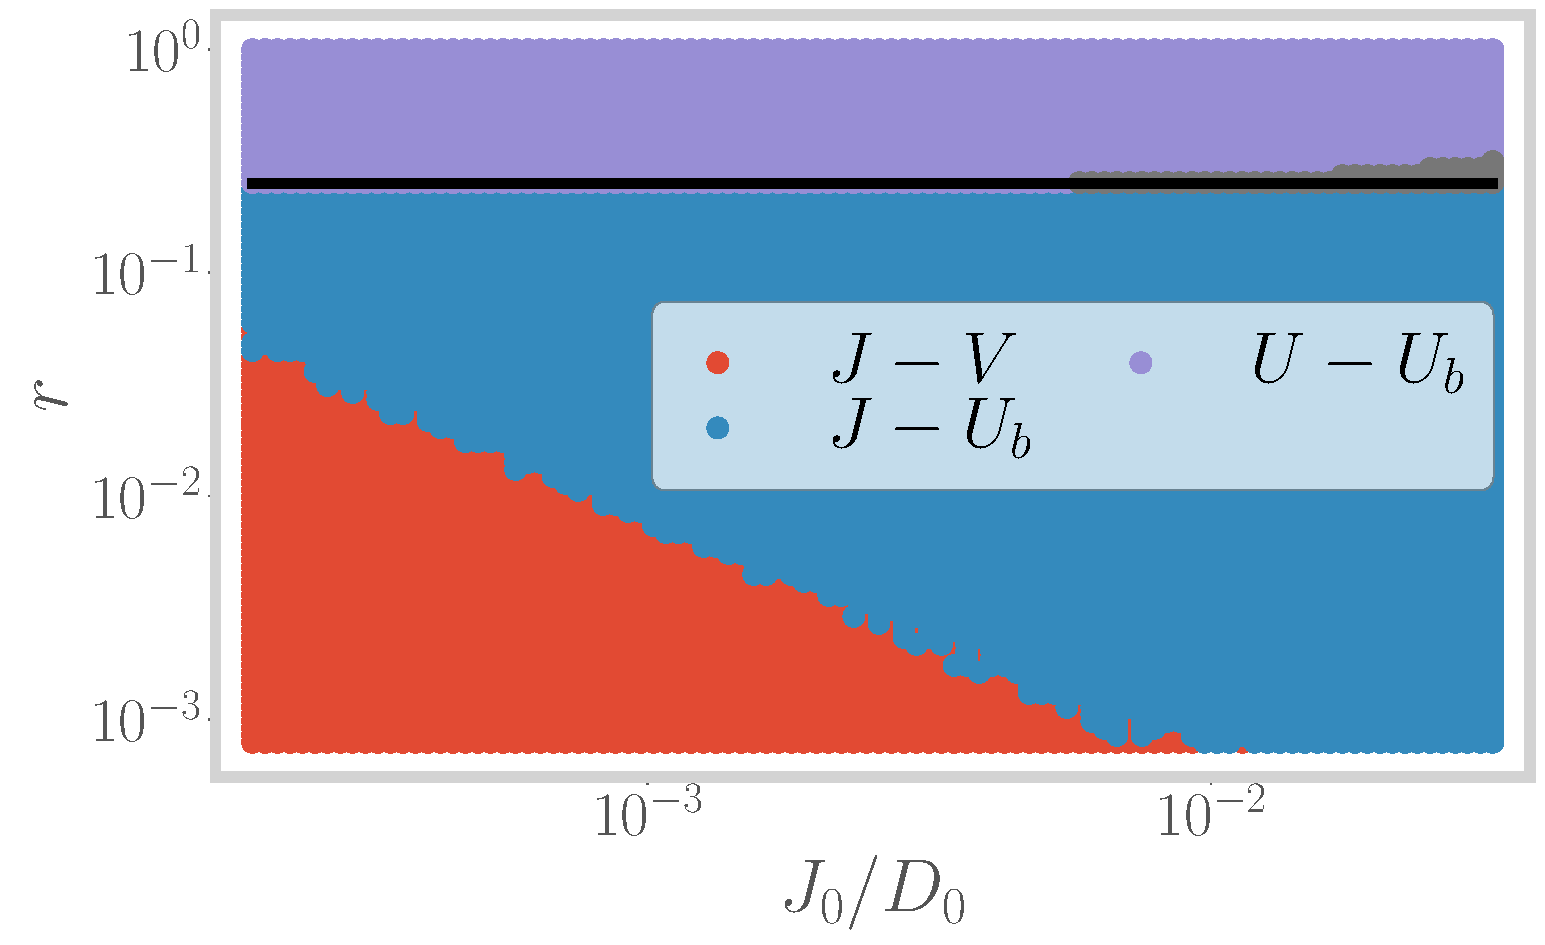
\includegraphics[width=0.48\textwidth]{../figures/phase-map-MIT.pdf}
	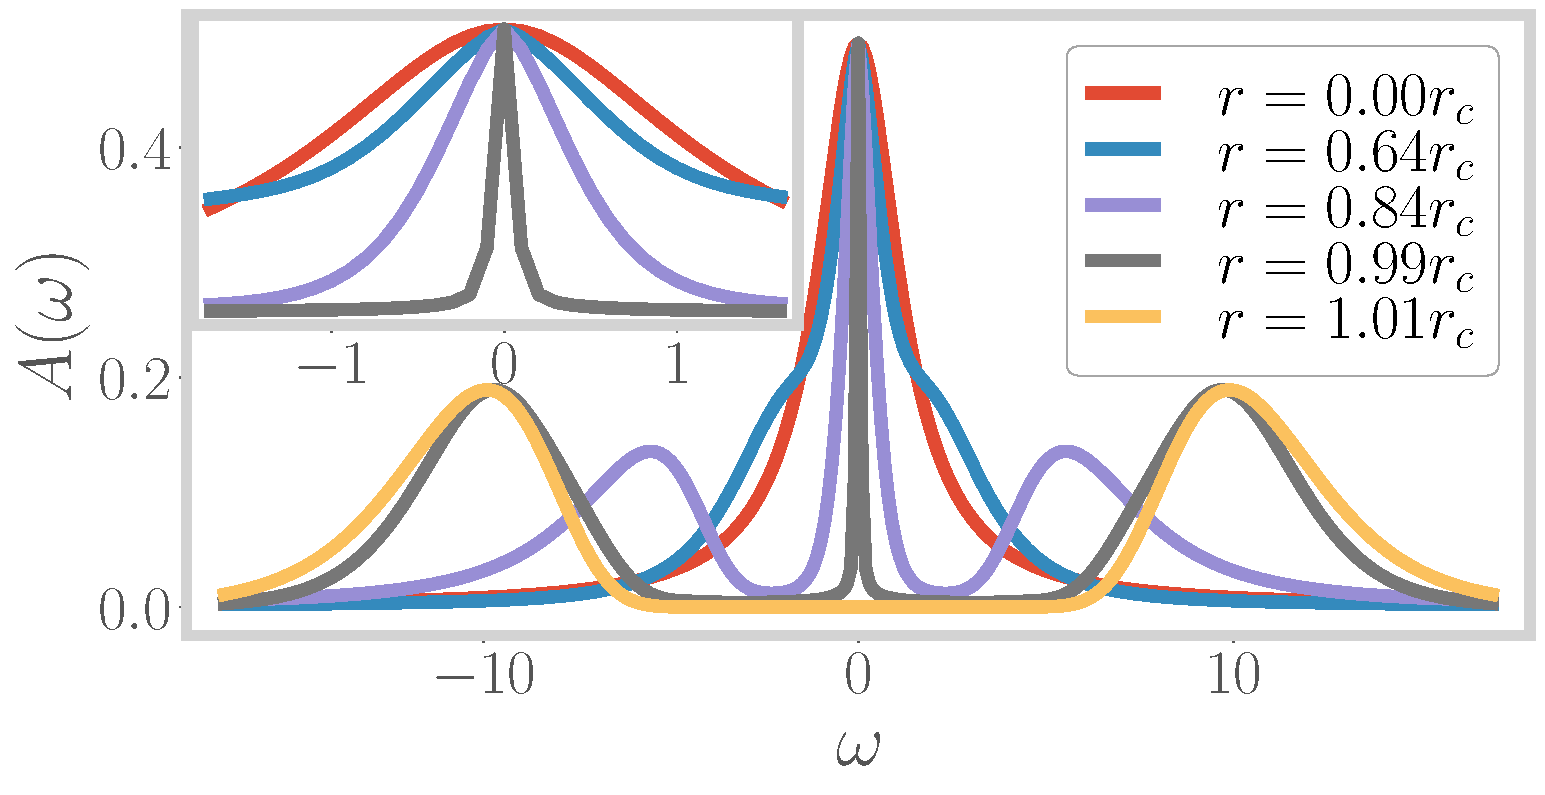
\includegraphics[width=0.48\textwidth]{../figures/spectral-function.pdf}
	\caption{{\it Left:} Phase diagram. {\it Right:} Impurity spectral function}
	\label{spec_func_mit}
\end{figure}

\item The impurity spectral function \(A_{dd}(\omega)\) and the impurity-bath real space off-diagonal Greens function \(A_{d0}(\omega)\) reveal a gap in the spectrum at low \(\omega\) for \(U_b > J/4\). The gap in the diagonal spectral function shows that the impurity site cannot fluctuate through gapless excitations, while the vanishing of the off-diagonal spectral function shows that an electron on the impurity site cannot delocalise out of that site.  Other measures like mutual information and spin-spin correlations also show a sharp change on crossing that value, demonstrating \textbf{the destruction of the Kondo cloud and the stabilisation of the local moment on the impurity}.

\begin{figure}[!htb]
\centering
	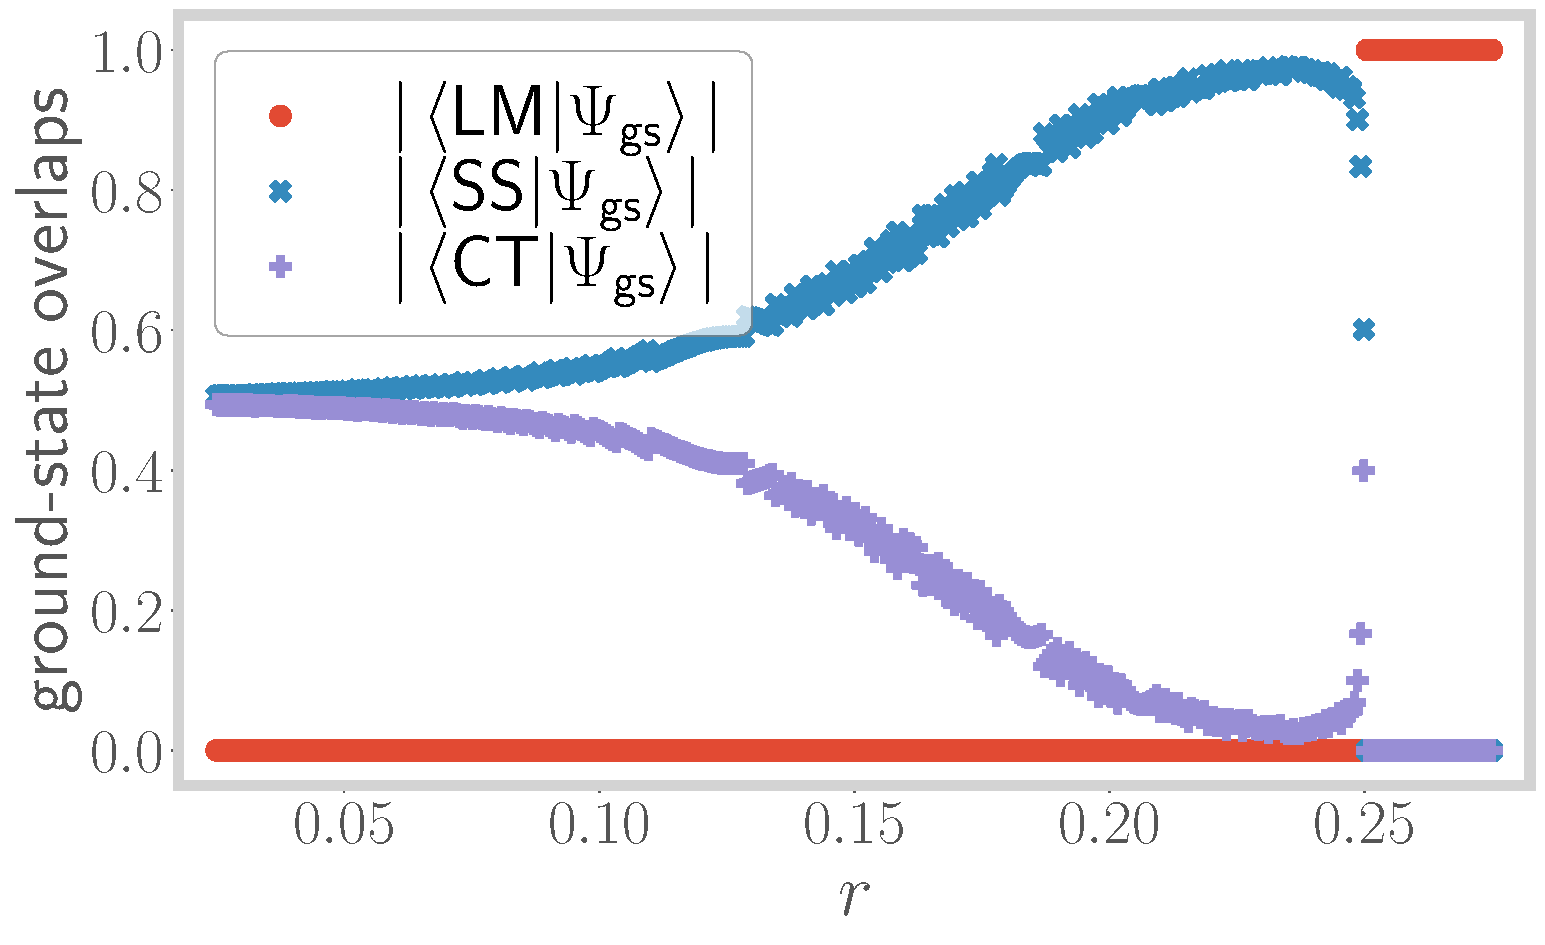
\includegraphics[width=0.48\textwidth]{../figures/corrs_gs.pdf}
	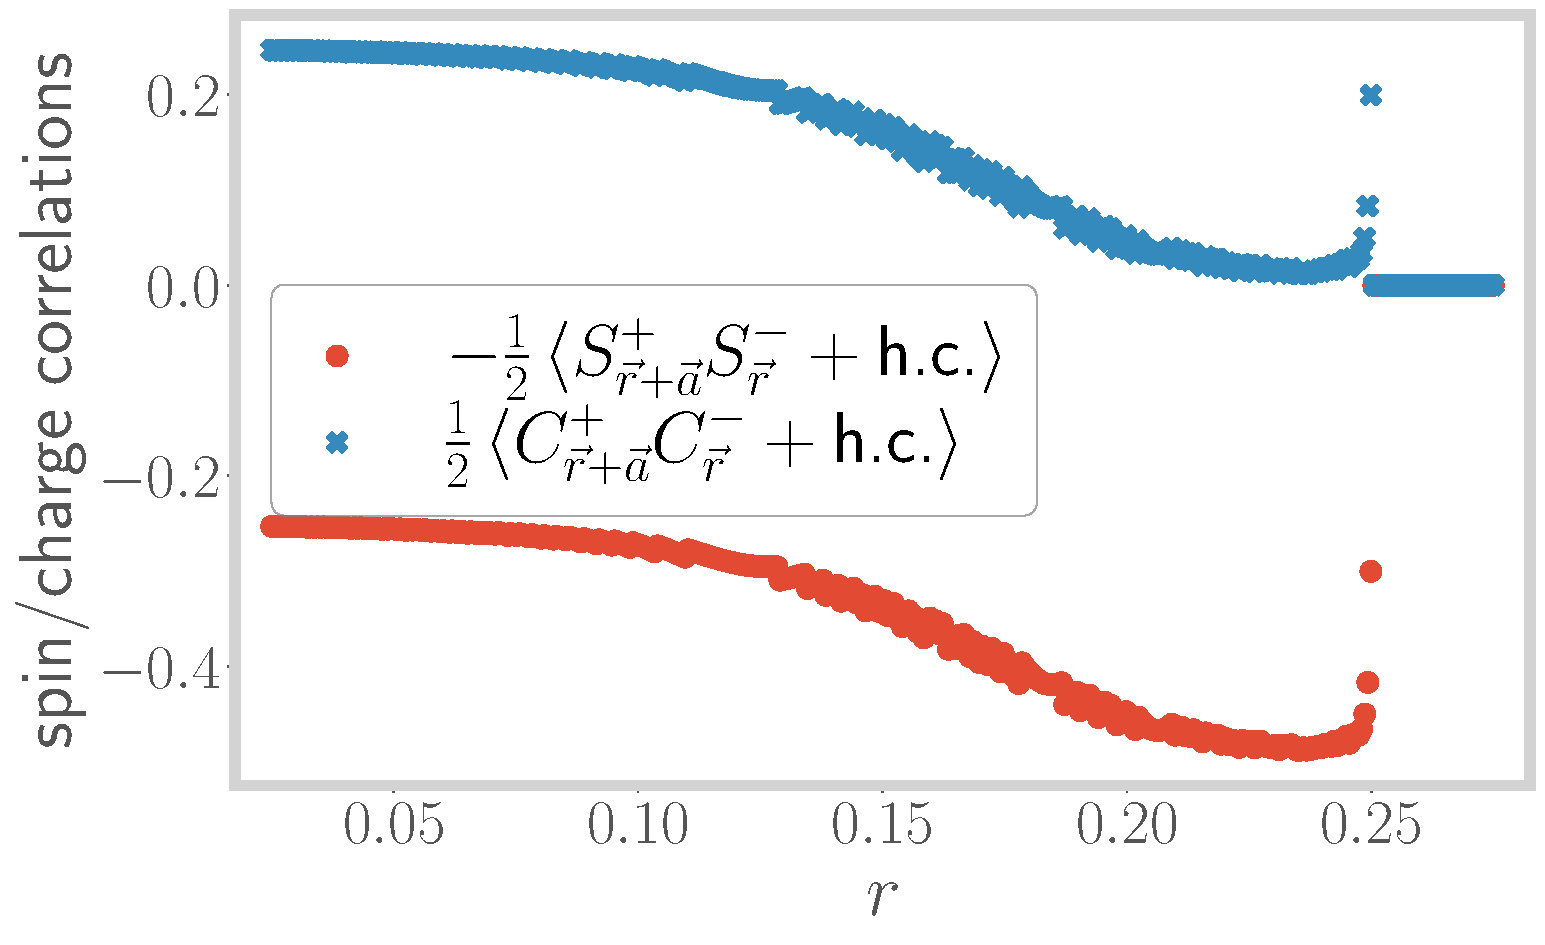
\includegraphics[width=0.48\textwidth]{../figures/spin-charge-corr-full.pdf}
	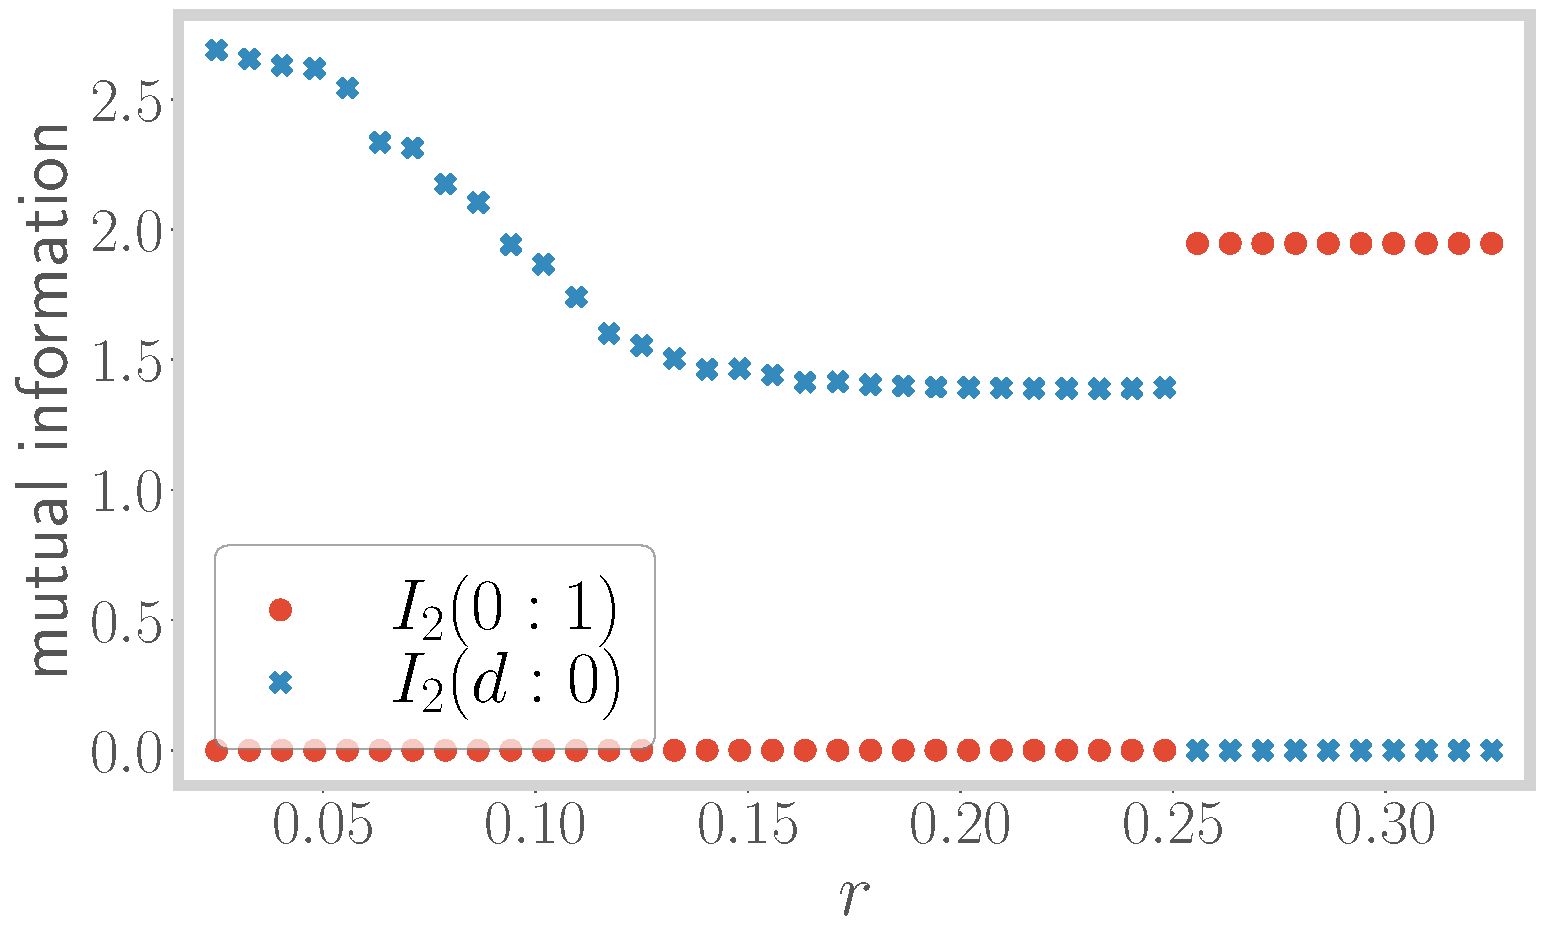
\includegraphics[width=0.48\textwidth]{../figures/mutinfo-d0-01-full.pdf}
	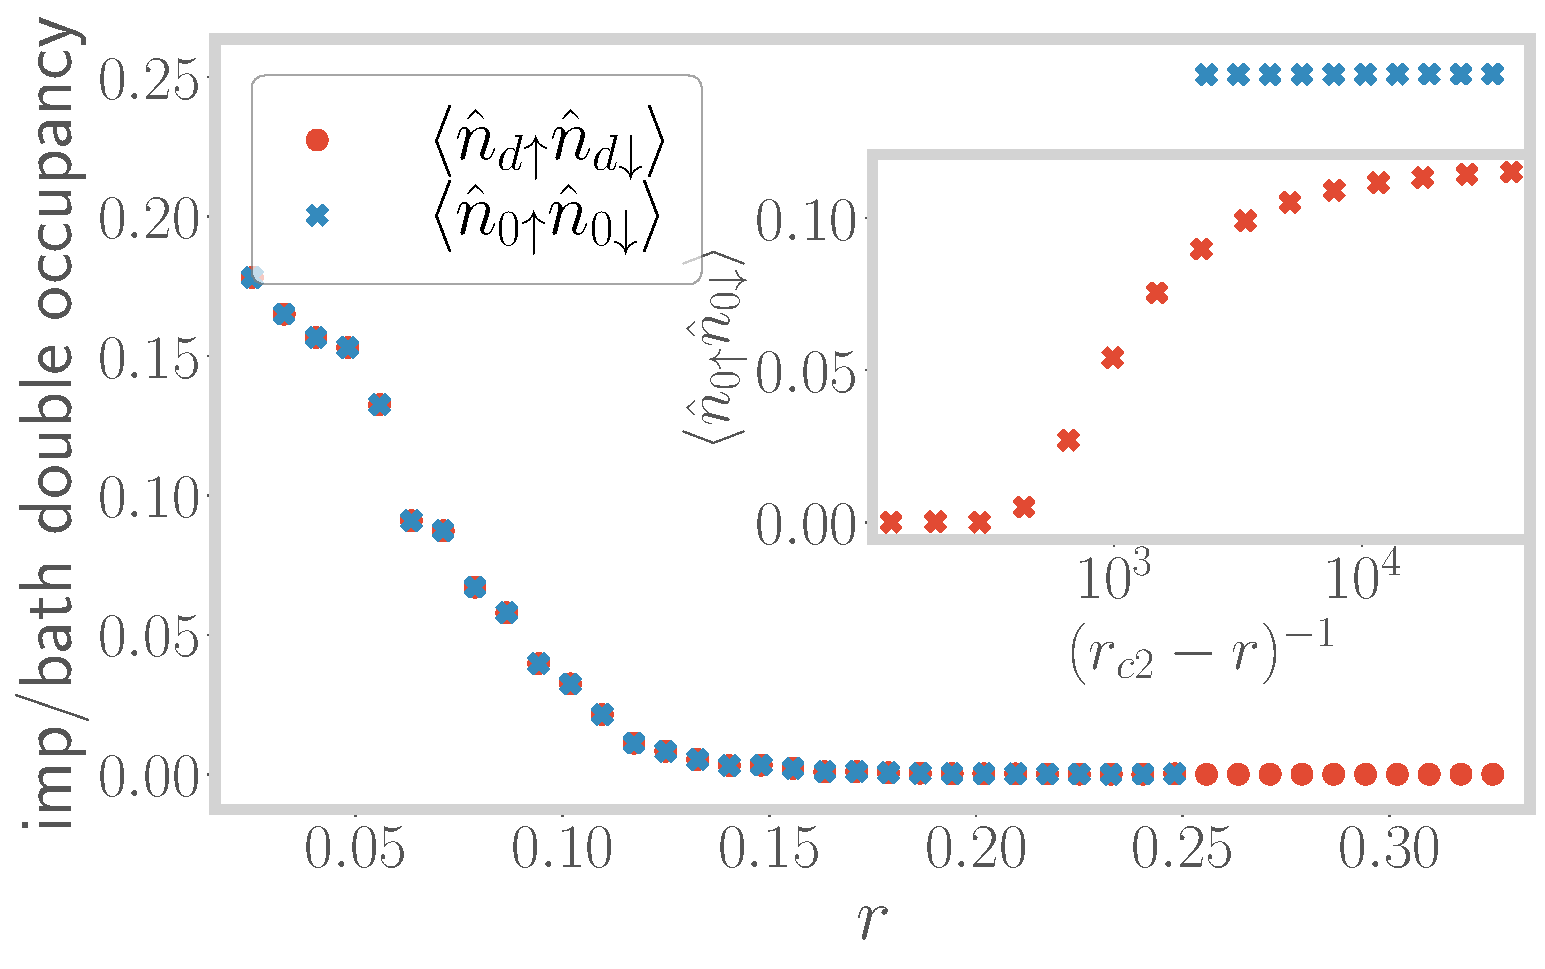
\includegraphics[width=0.48\textwidth]{../figures/doub_occ.pdf}
\end{figure}

	\item In the context of the auxiliary model, this represents an \textbf{impurity phase transition} from the completely-screened spin-singlet phase to the unscreened local moment phase.

Using the mappings between the auxiliary model parameters and the bulk parameters (eq.~\ref{map_aux_bulk}), one can define a critical value \(r^{*}\) of the ratio \(r = U_{H-H}/J_{H-H}\) at the critical points \(-U_b/J=1/4\) \textit{for a given and fixed value of \(U\)}. We will now argue that this critical point describes a metal-insulator transition. For \(r < r^{*}\), the well-defined low-\(\omega\) central peak in the impurity spectral function, as well as the large mutual and information correlations, in the ground state, among the members of the Kondo cloud or between the impurity and the zeroth site show that the impurity and the bath are very strongly entangled, and the weighted poles \(\left(|d^p_n|^2 + \left(d^p_n\right)^* z^p_n\right) \left(\mathcal{G}_\text{aux}(d, \omega)\right)_{nn}\) and \(\left(|d^h_n|^2 + \left(z^h_n\right)^* d^h_n\right)\left(\mathcal{G}_\text{aux}(d, -\omega)\right)_{nn}\) are non-zero at low \(\omega\). This means that both the local and the nearest-neighbour Greens functions, that are related to these parameters via eq.~\ref{greens_func_siam}, have poles at low\(-\omega\) and support the propagation of electrons through gapless excitations. Since the spectral function is also very simply related to that of the auxiliary model (eq.\eqref{main}), the former also shows the same zero-energy resonance.

On the other side \(r > r^{*}\) of the critical point, we know that the impurity gets decoupled from the bath, such that the weighted poles \(\left(|d^p_n|^2 + \left(d^p_n\right)^* z^p_n\right) \left(\mathcal{G}_\text{aux}(d, \omega)\right)_{nn}\) and \(\left(|d^h_n|^2 + \left(z^h_n\right)^* d^h_n\right)\left(\mathcal{G}_\text{aux}(d, -\omega)\right)_{nn}\) vanish. This is simply the loss of spectral weight at low-\(\omega\) because of the removal of the gapless excitations, and is demonstrated through the impurity spectral function in fig.~\ref{spec_func_mit}. This then implies that the bulk Greens functions will also gap out at low energies, and that describes an insulating phase where the electrons get "jammed" in the local states. By the same argument as above, the bulk spectral function also sees a gap in this phase when the impurity spectral function is gapped (see eq.\eqref{main}).

Finally, using eqs.\eqref{map_aux_bulk} and the criticality condition $U_{b}^{*}=-\frac{J^{*}}{4}$, we can offer a functional form for the critical value of the parameter $r^{*} = U_{H-H}^{*}/J_{H-H}^{*}$
\begin{eqnarray}
r^{*} &=& \frac{U_{H-H}^{*}}{J_{H-H}^{*}} = \frac{w}{4}\left(\frac{U^{*}}{J^{*}} - \frac{1}{2}\right)
\end{eqnarray}
where $U^{*}$ and $J^{*}$ are the values of the on-site and Kondo couplings of the auxiliary model at the auxiliary model (i.e., the generalised SIAM with a correlated bath) at the transition between the Kondo screened and the local moment phases. Parametrising the bath correlation coupling as $U_{b}=-\frac{U}{10}$, we obtain $U^{*}/J^{*}=5/2$, and $r^{*} = 2$ for the 2D square lattice Hubbard-Heisenberg model (with coordination number $w=4$). In general, $w=2d$ for the $d$-dimensional hypercubic lattice, and 
$r^{*}_\text{hyperc.} = \frac{d}{2}\left(\frac{U^{*}}{J^{*}} - \frac{1}{2}\right)$. The growth of $r^{*}$ with $d$ indicates that the MIT is increasingly rendered difficult in a higher dimensional hypercubic lattice, as it is easier for electrons to delocalise and a very large on-site repulsion is needed to overcome this.
\end{itemize}

\comment{
\section{\(k-\)space picture of the MIT in terms of the momentum-resolved self-energy \(\Sigma(\vec k,\omega)\)}

From the self-energy expressions obtained above, one can track the self-energy of the lattice model through the metal-insulator transition. In fig.~\ref{four-self}, we have provided these plots at specific values of \(U_b/J\) to show how the transition plays out in the Brillouin zone. {\it These plots can also be viewed as a video \href{https://abhirup-m.github.io/misc-sigma/}{\underline{here}}.}

\begin{center}
\begin{tabular}{c|c}
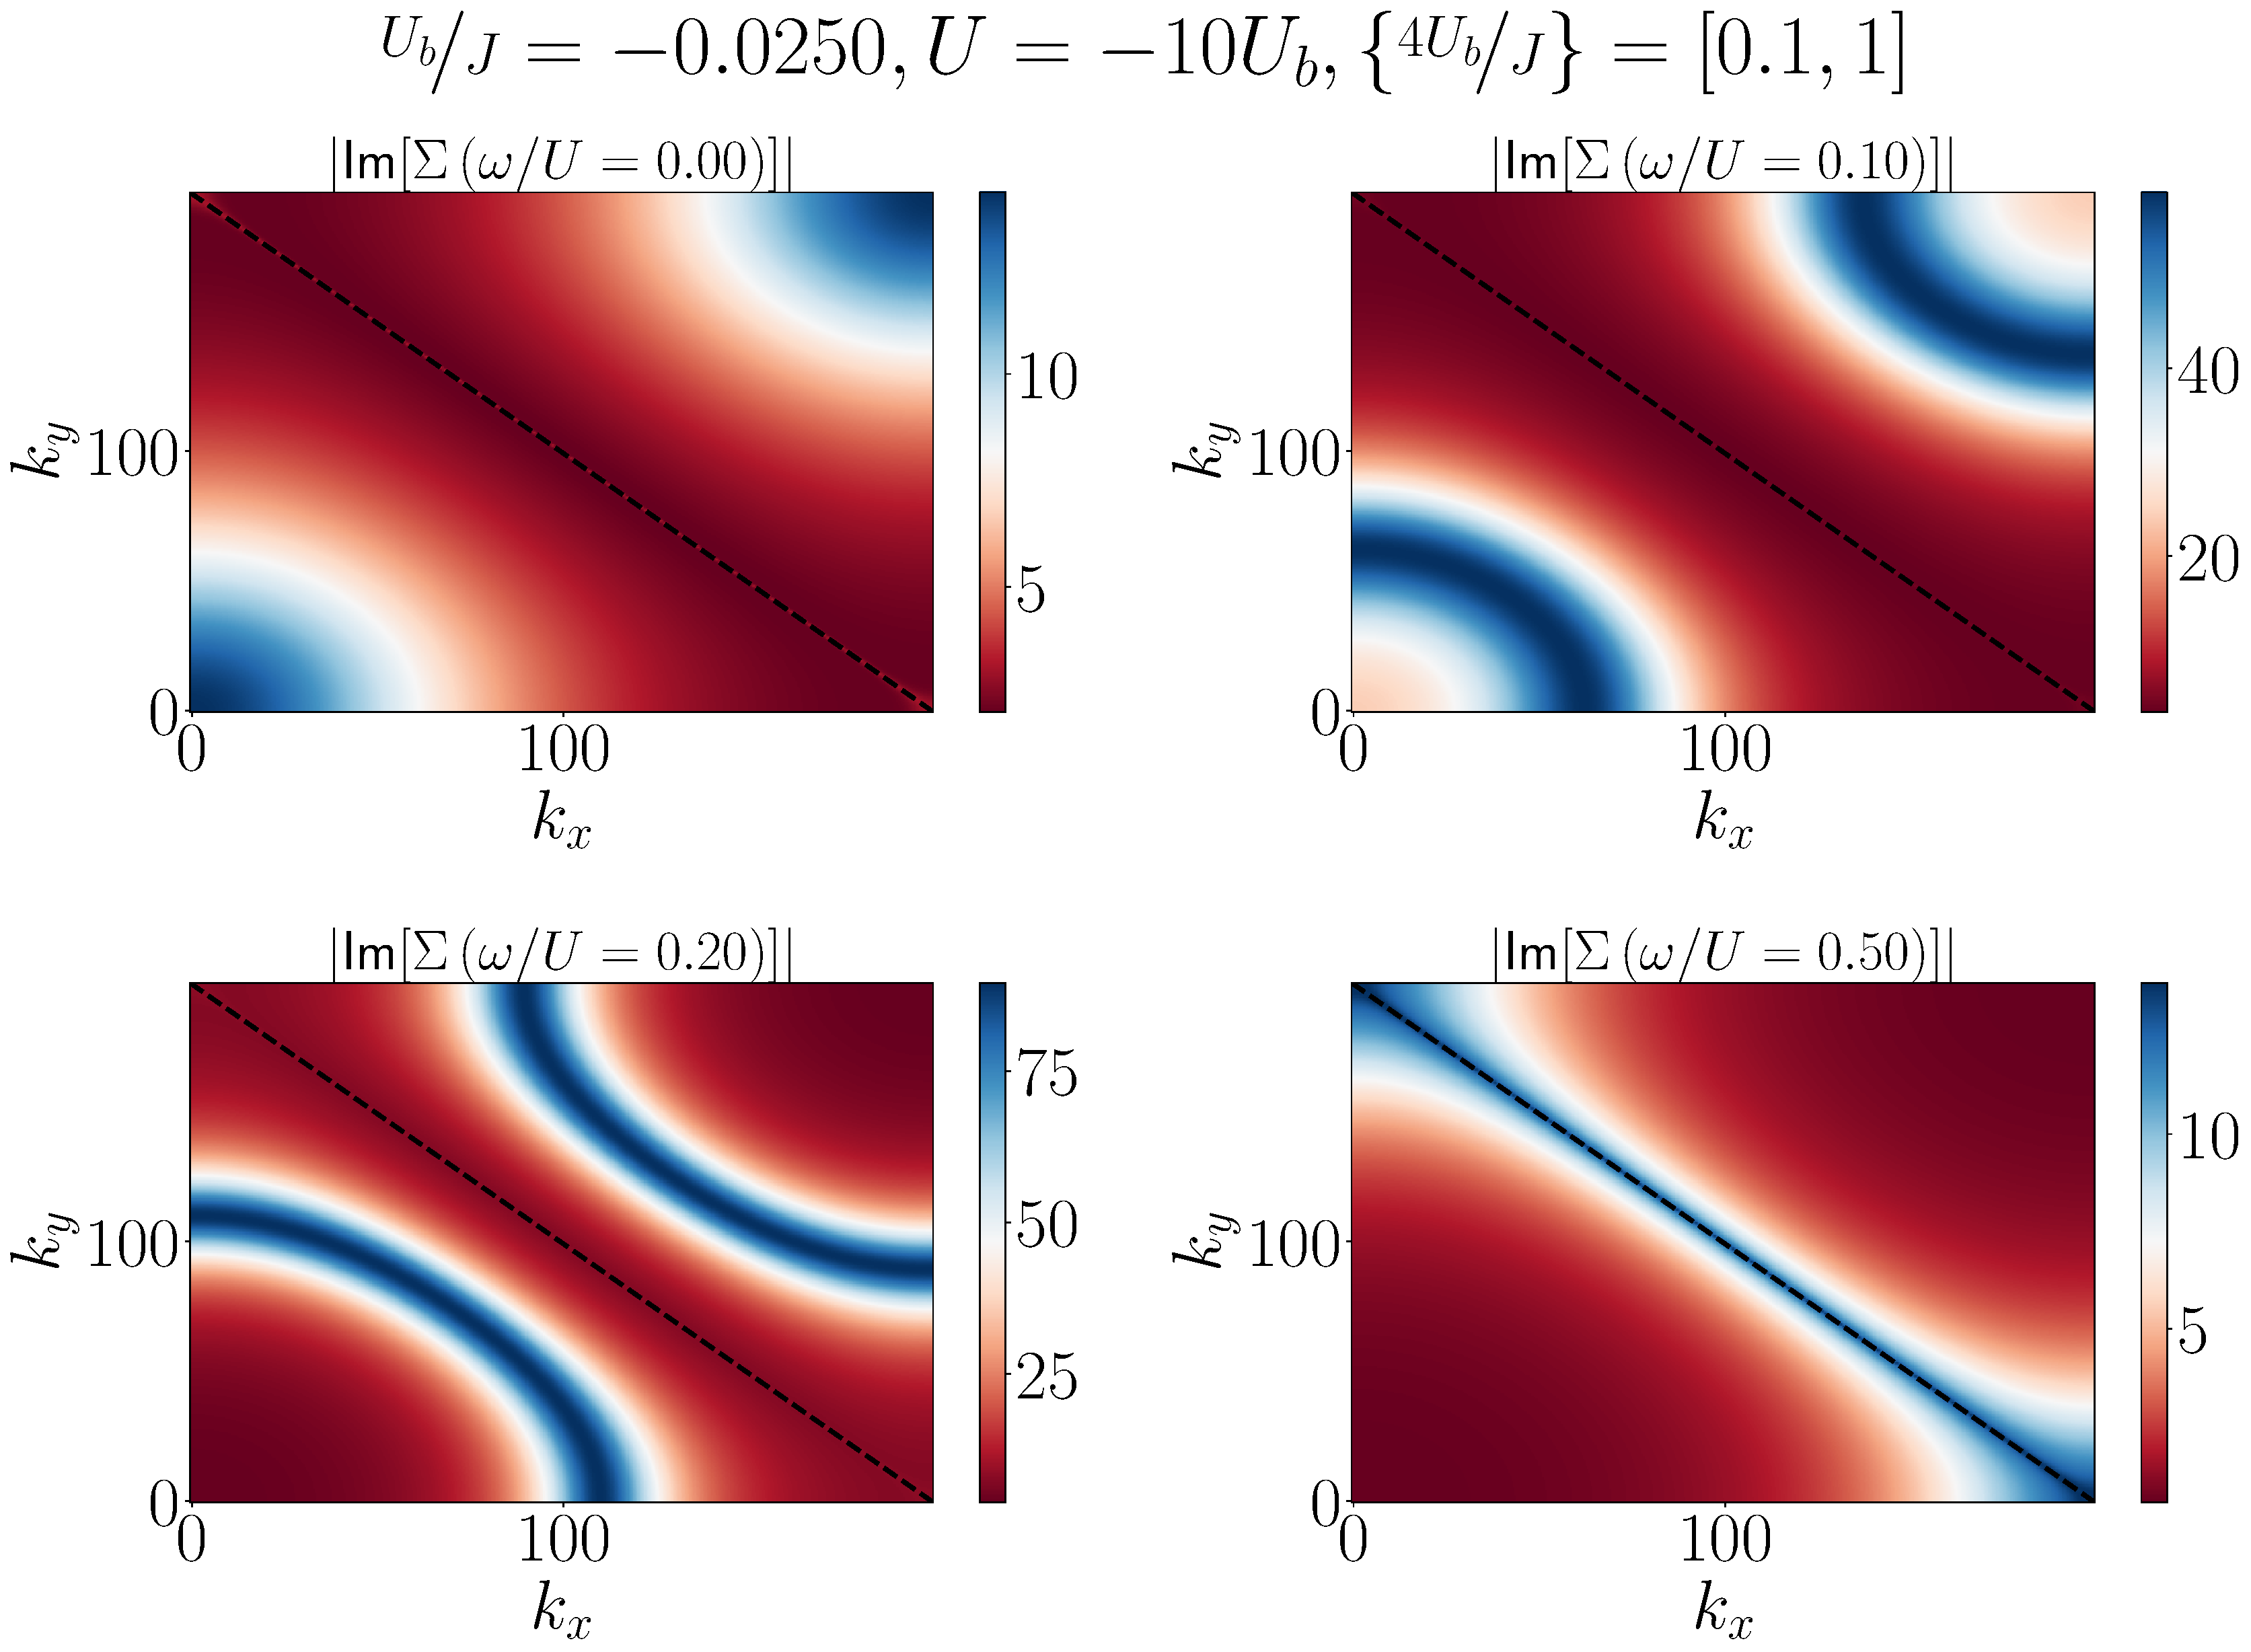
\includegraphics[height=0.3\textheight]{../figures/sigma-4-Ub_by_J=-0.02500-4.pdf} &
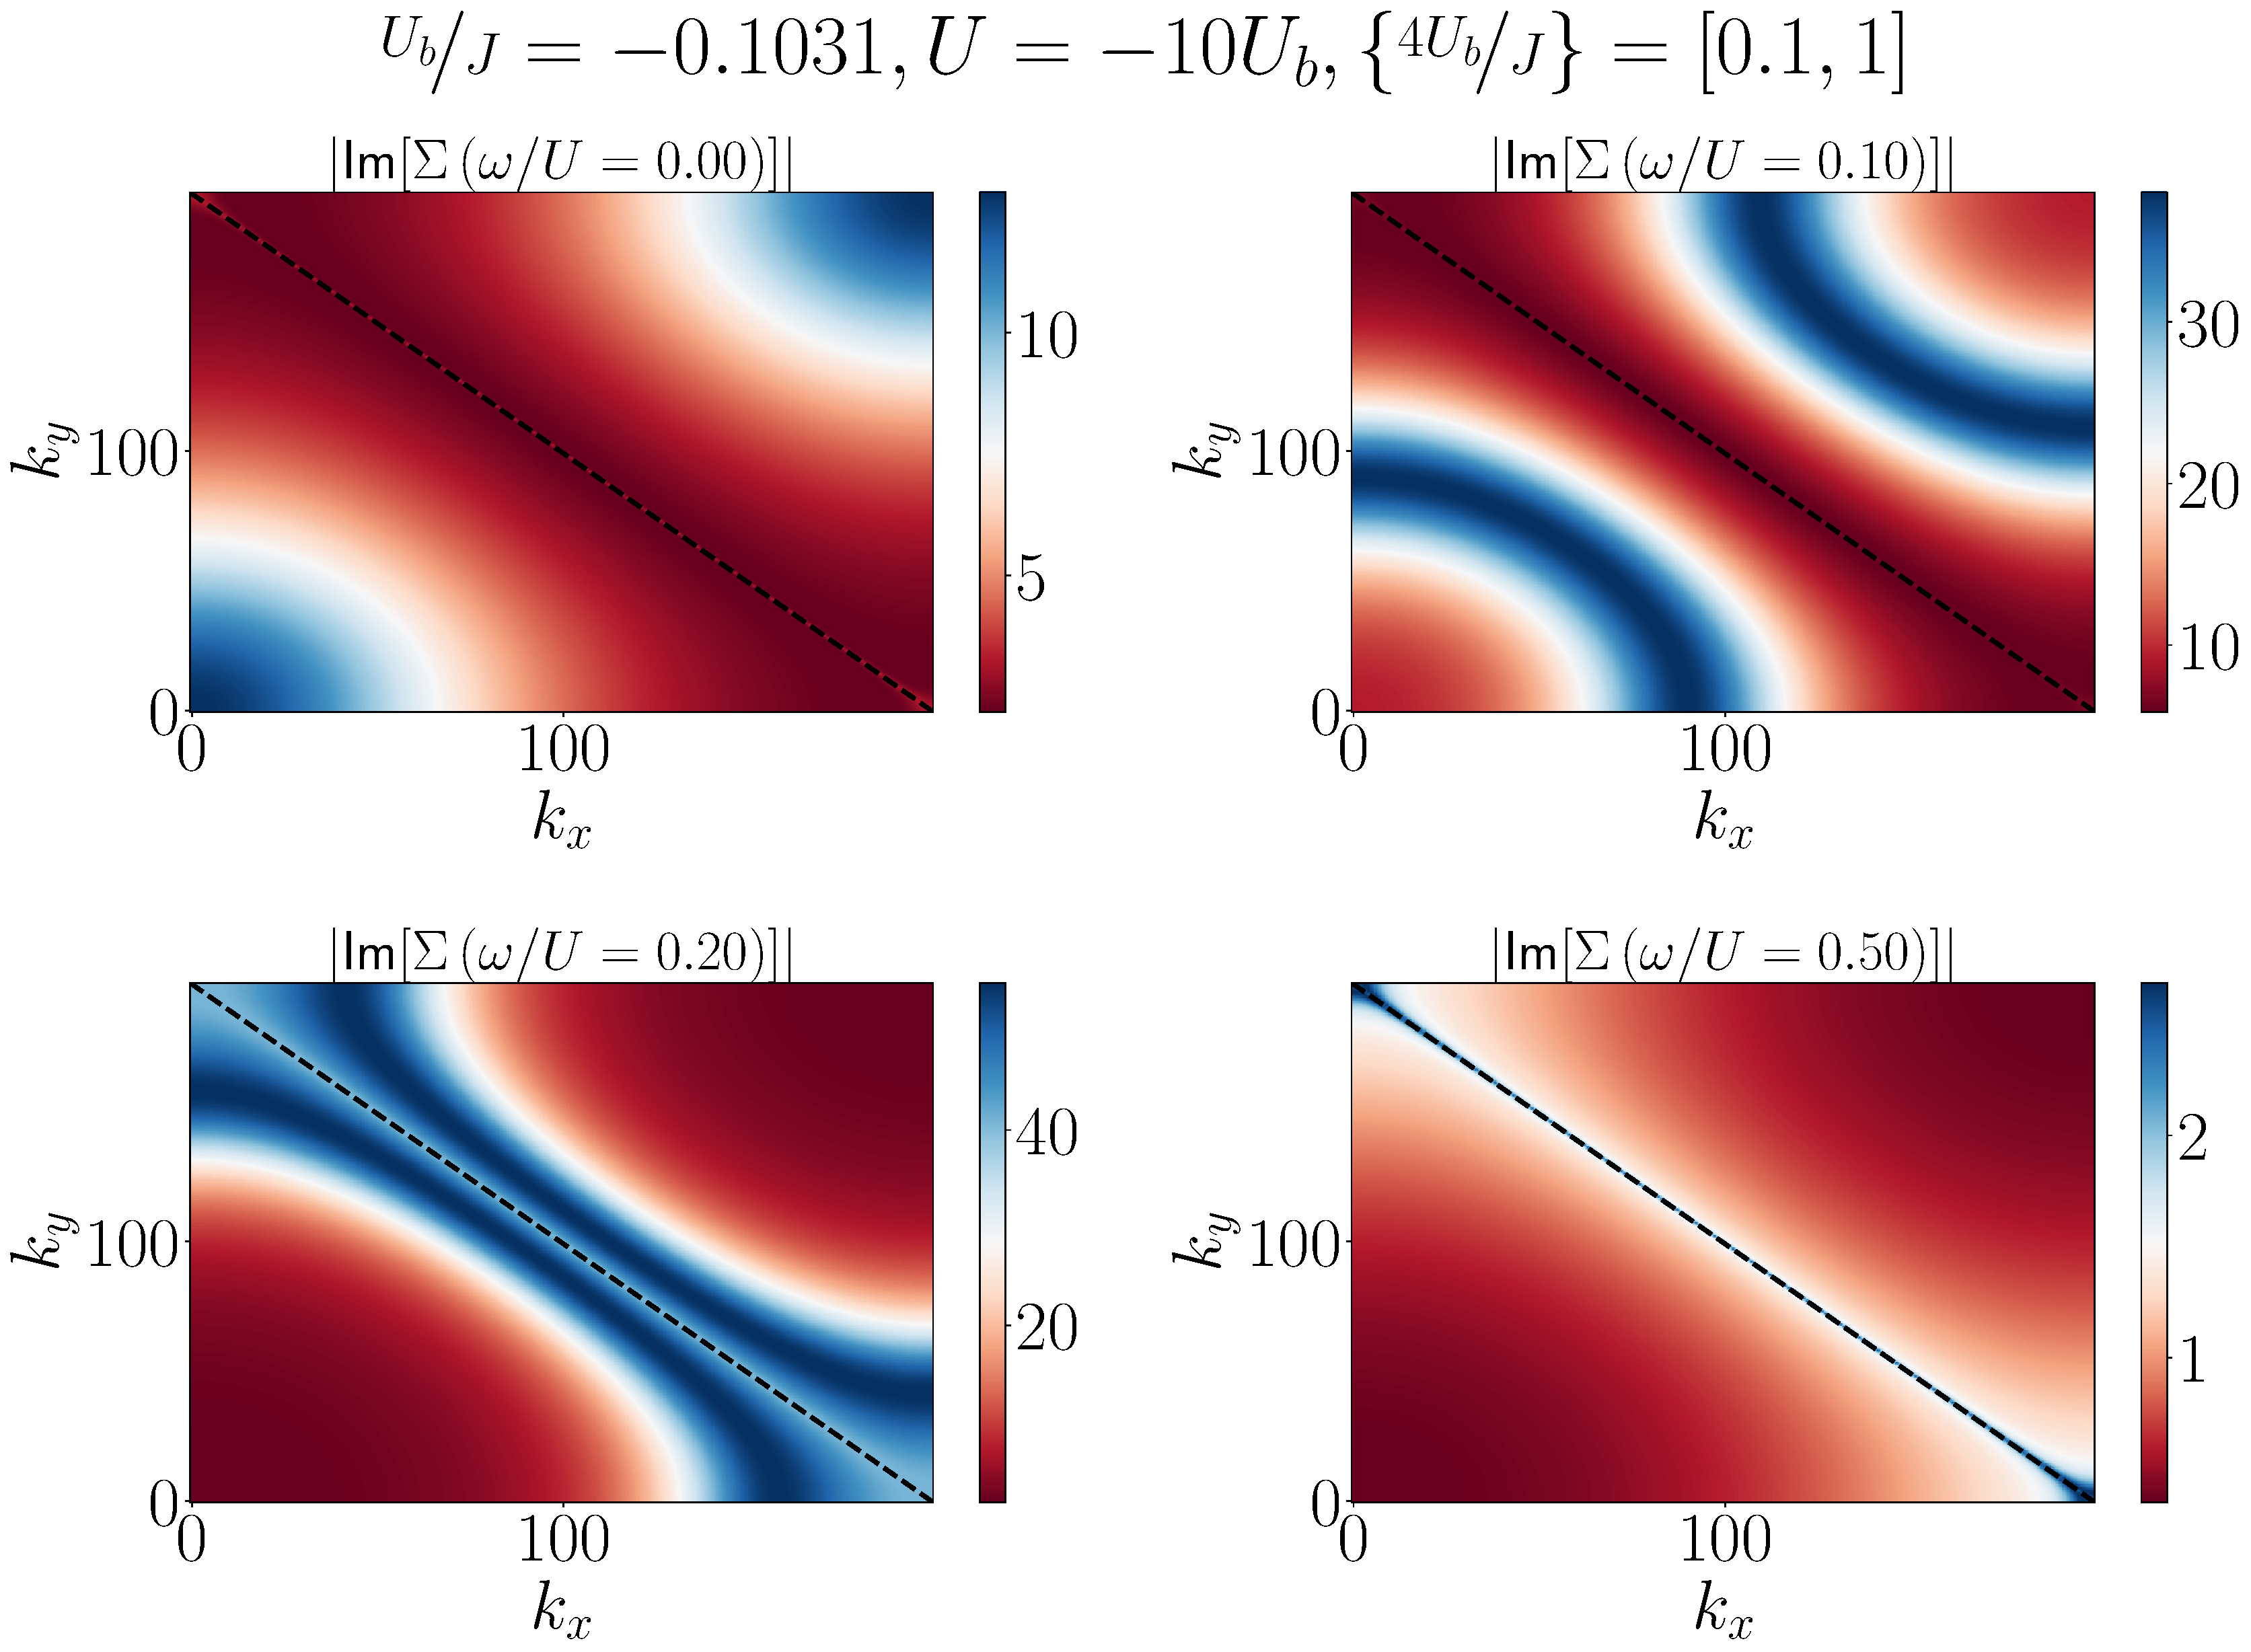
\includegraphics[height=0.3\textheight]{../figures/sigma-4-Ub_by_J=-0.10310-4.pdf}\\
\hline
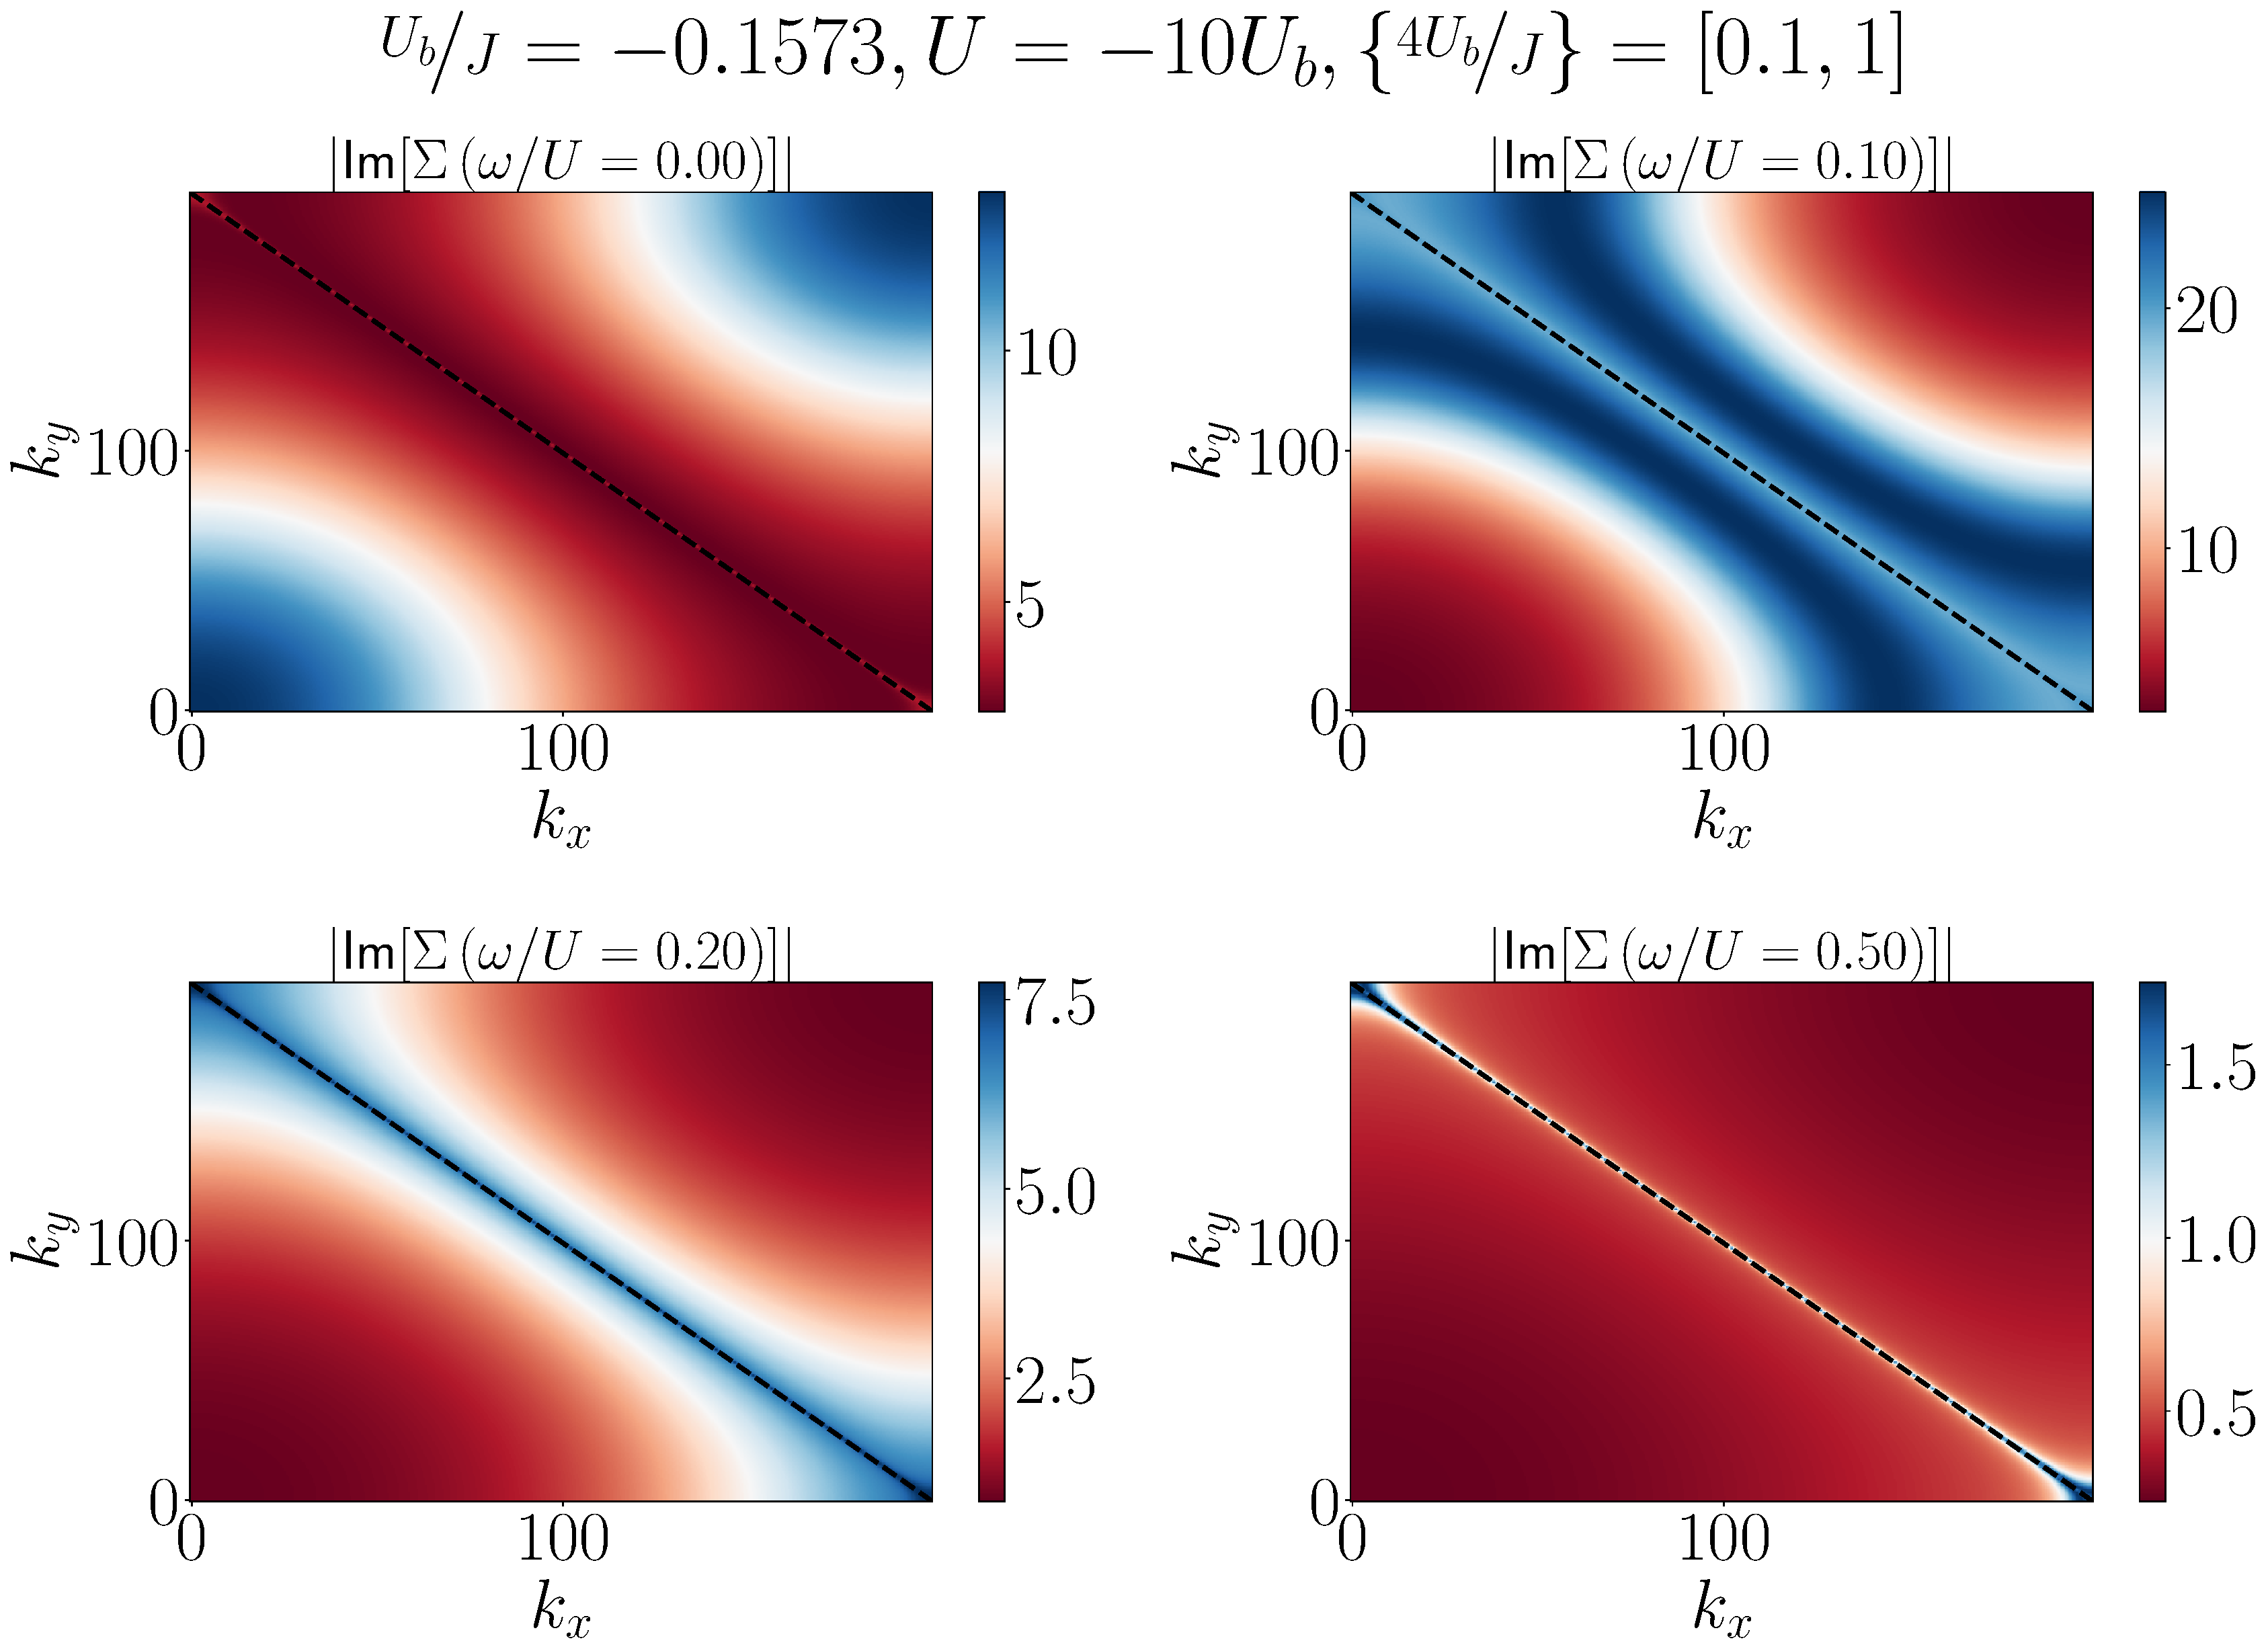
\includegraphics[height=0.3\textheight]{../figures/sigma-4-Ub_by_J=-0.15735-4.pdf} &
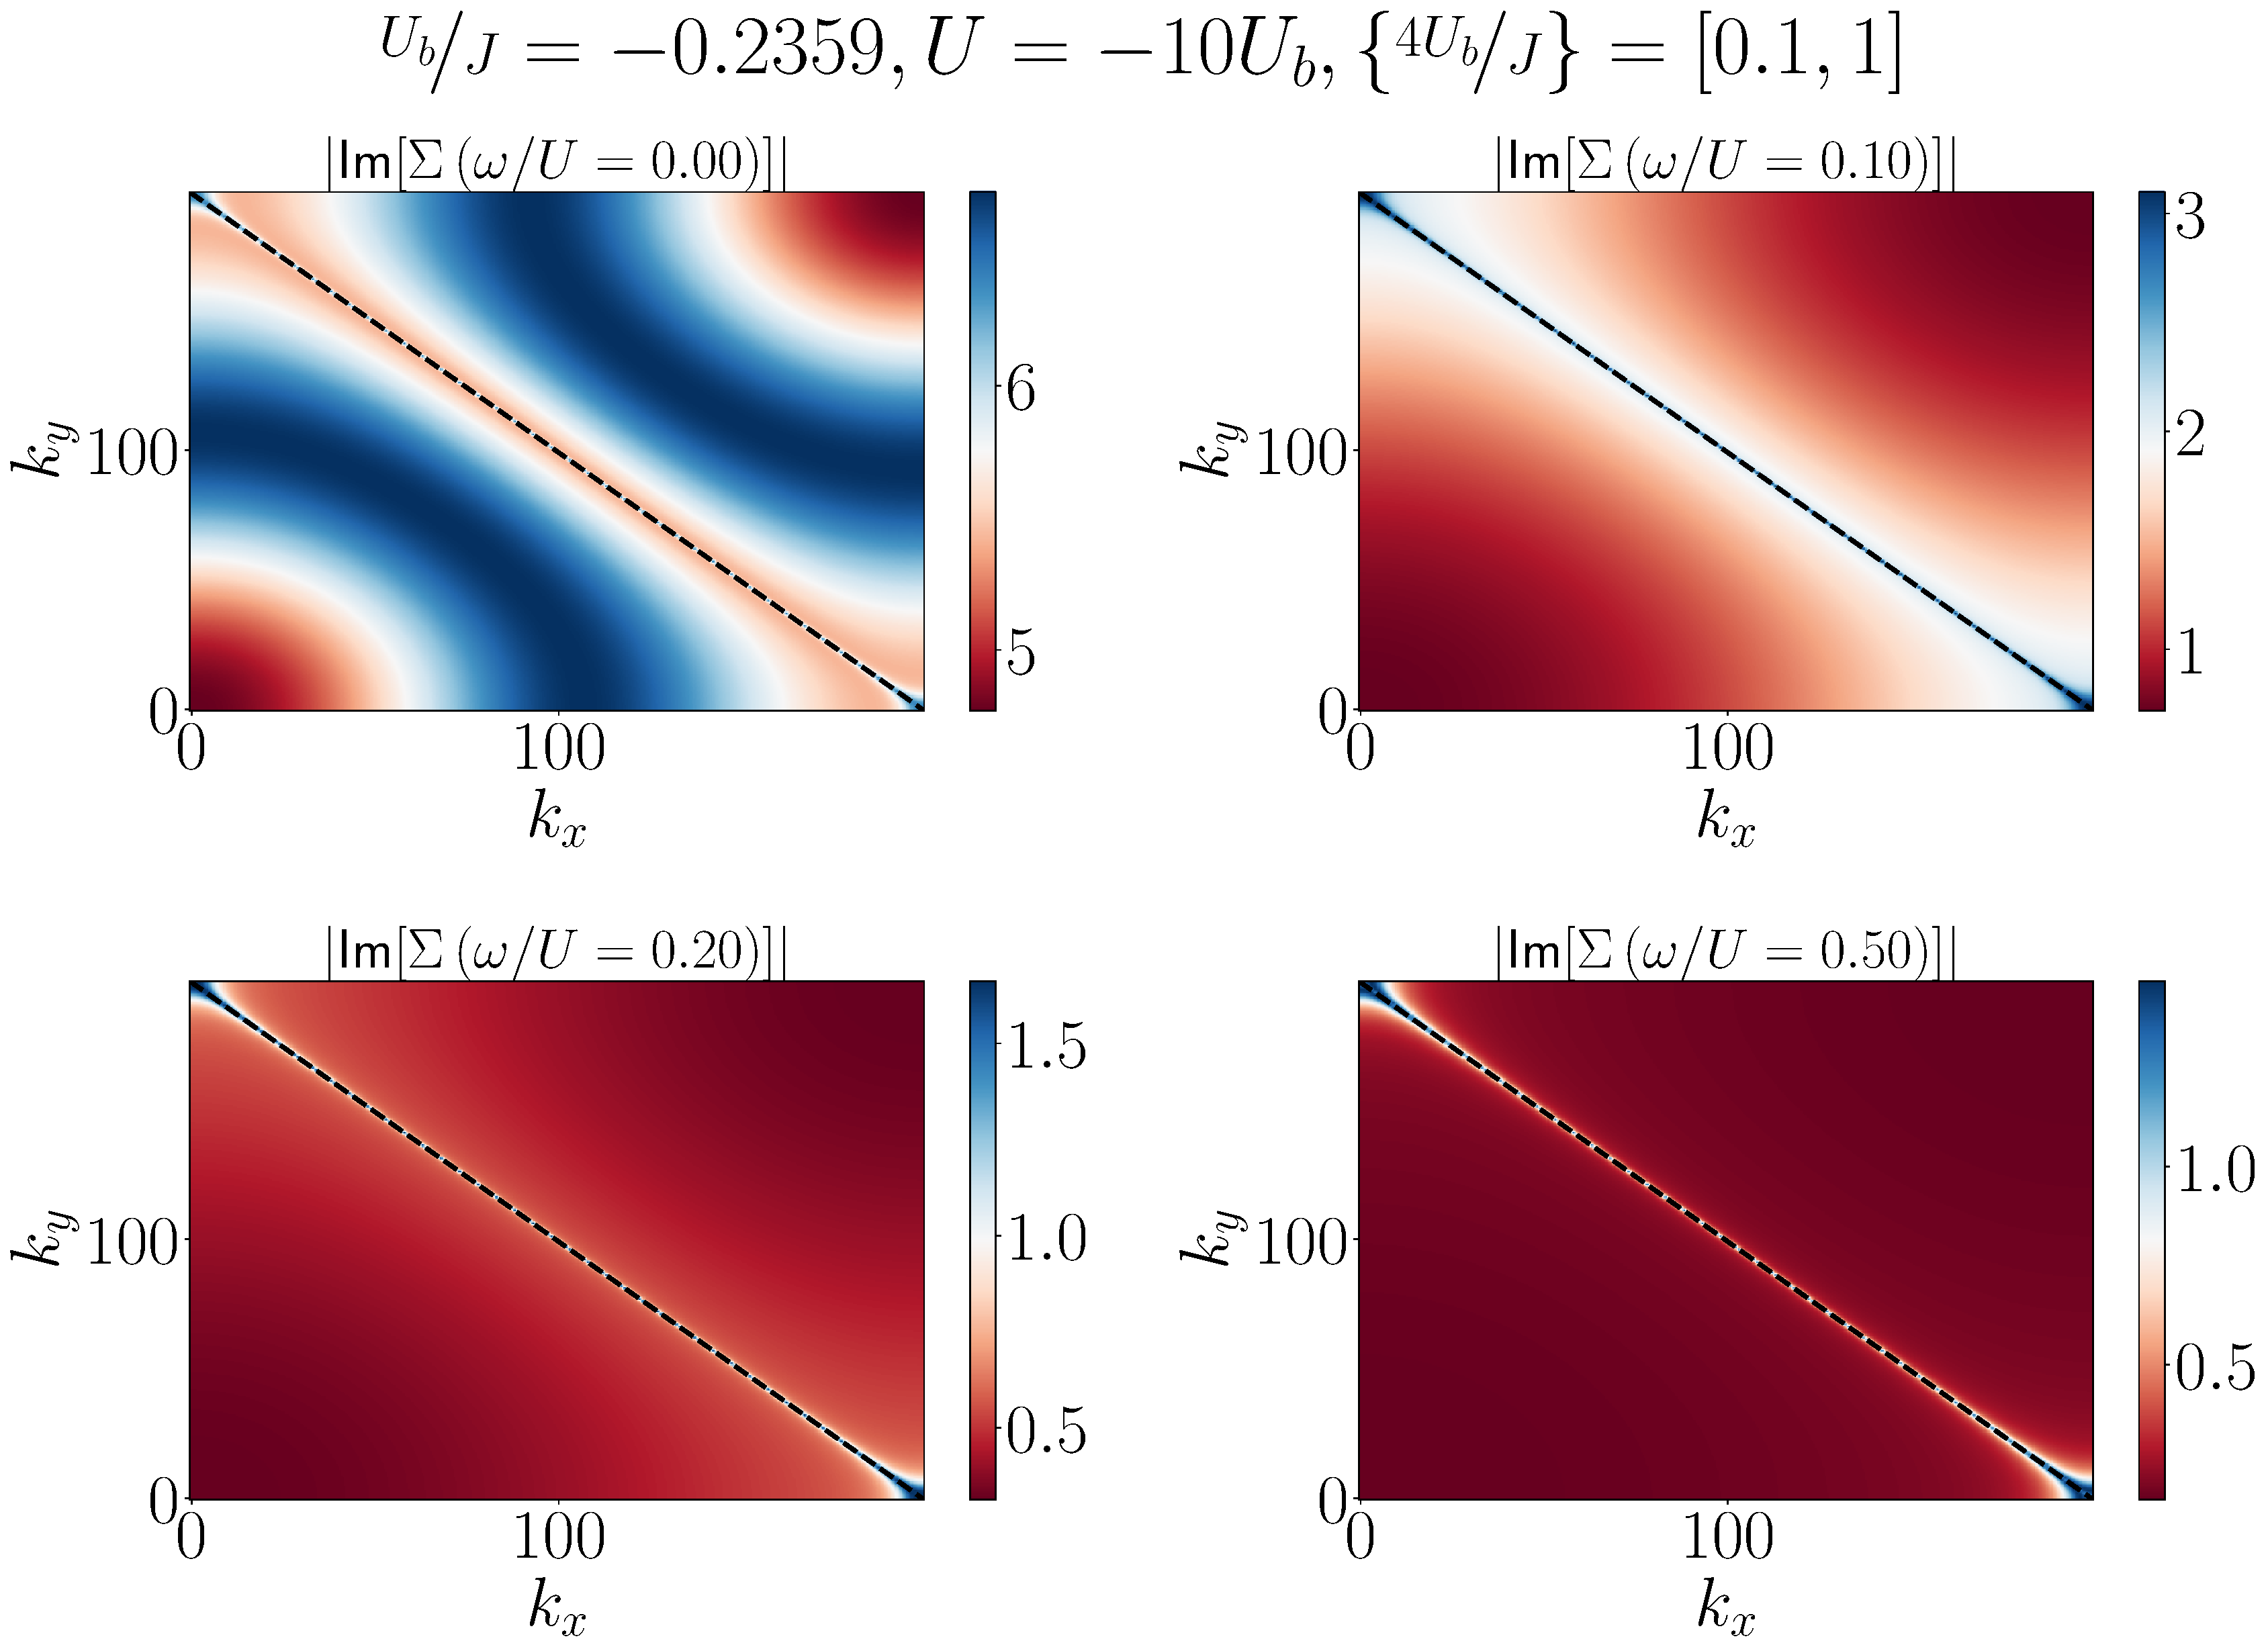
\includegraphics[height=0.3\textheight]{../figures/sigma-4-Ub_by_J=-0.23594-4.pdf}\\
\hline
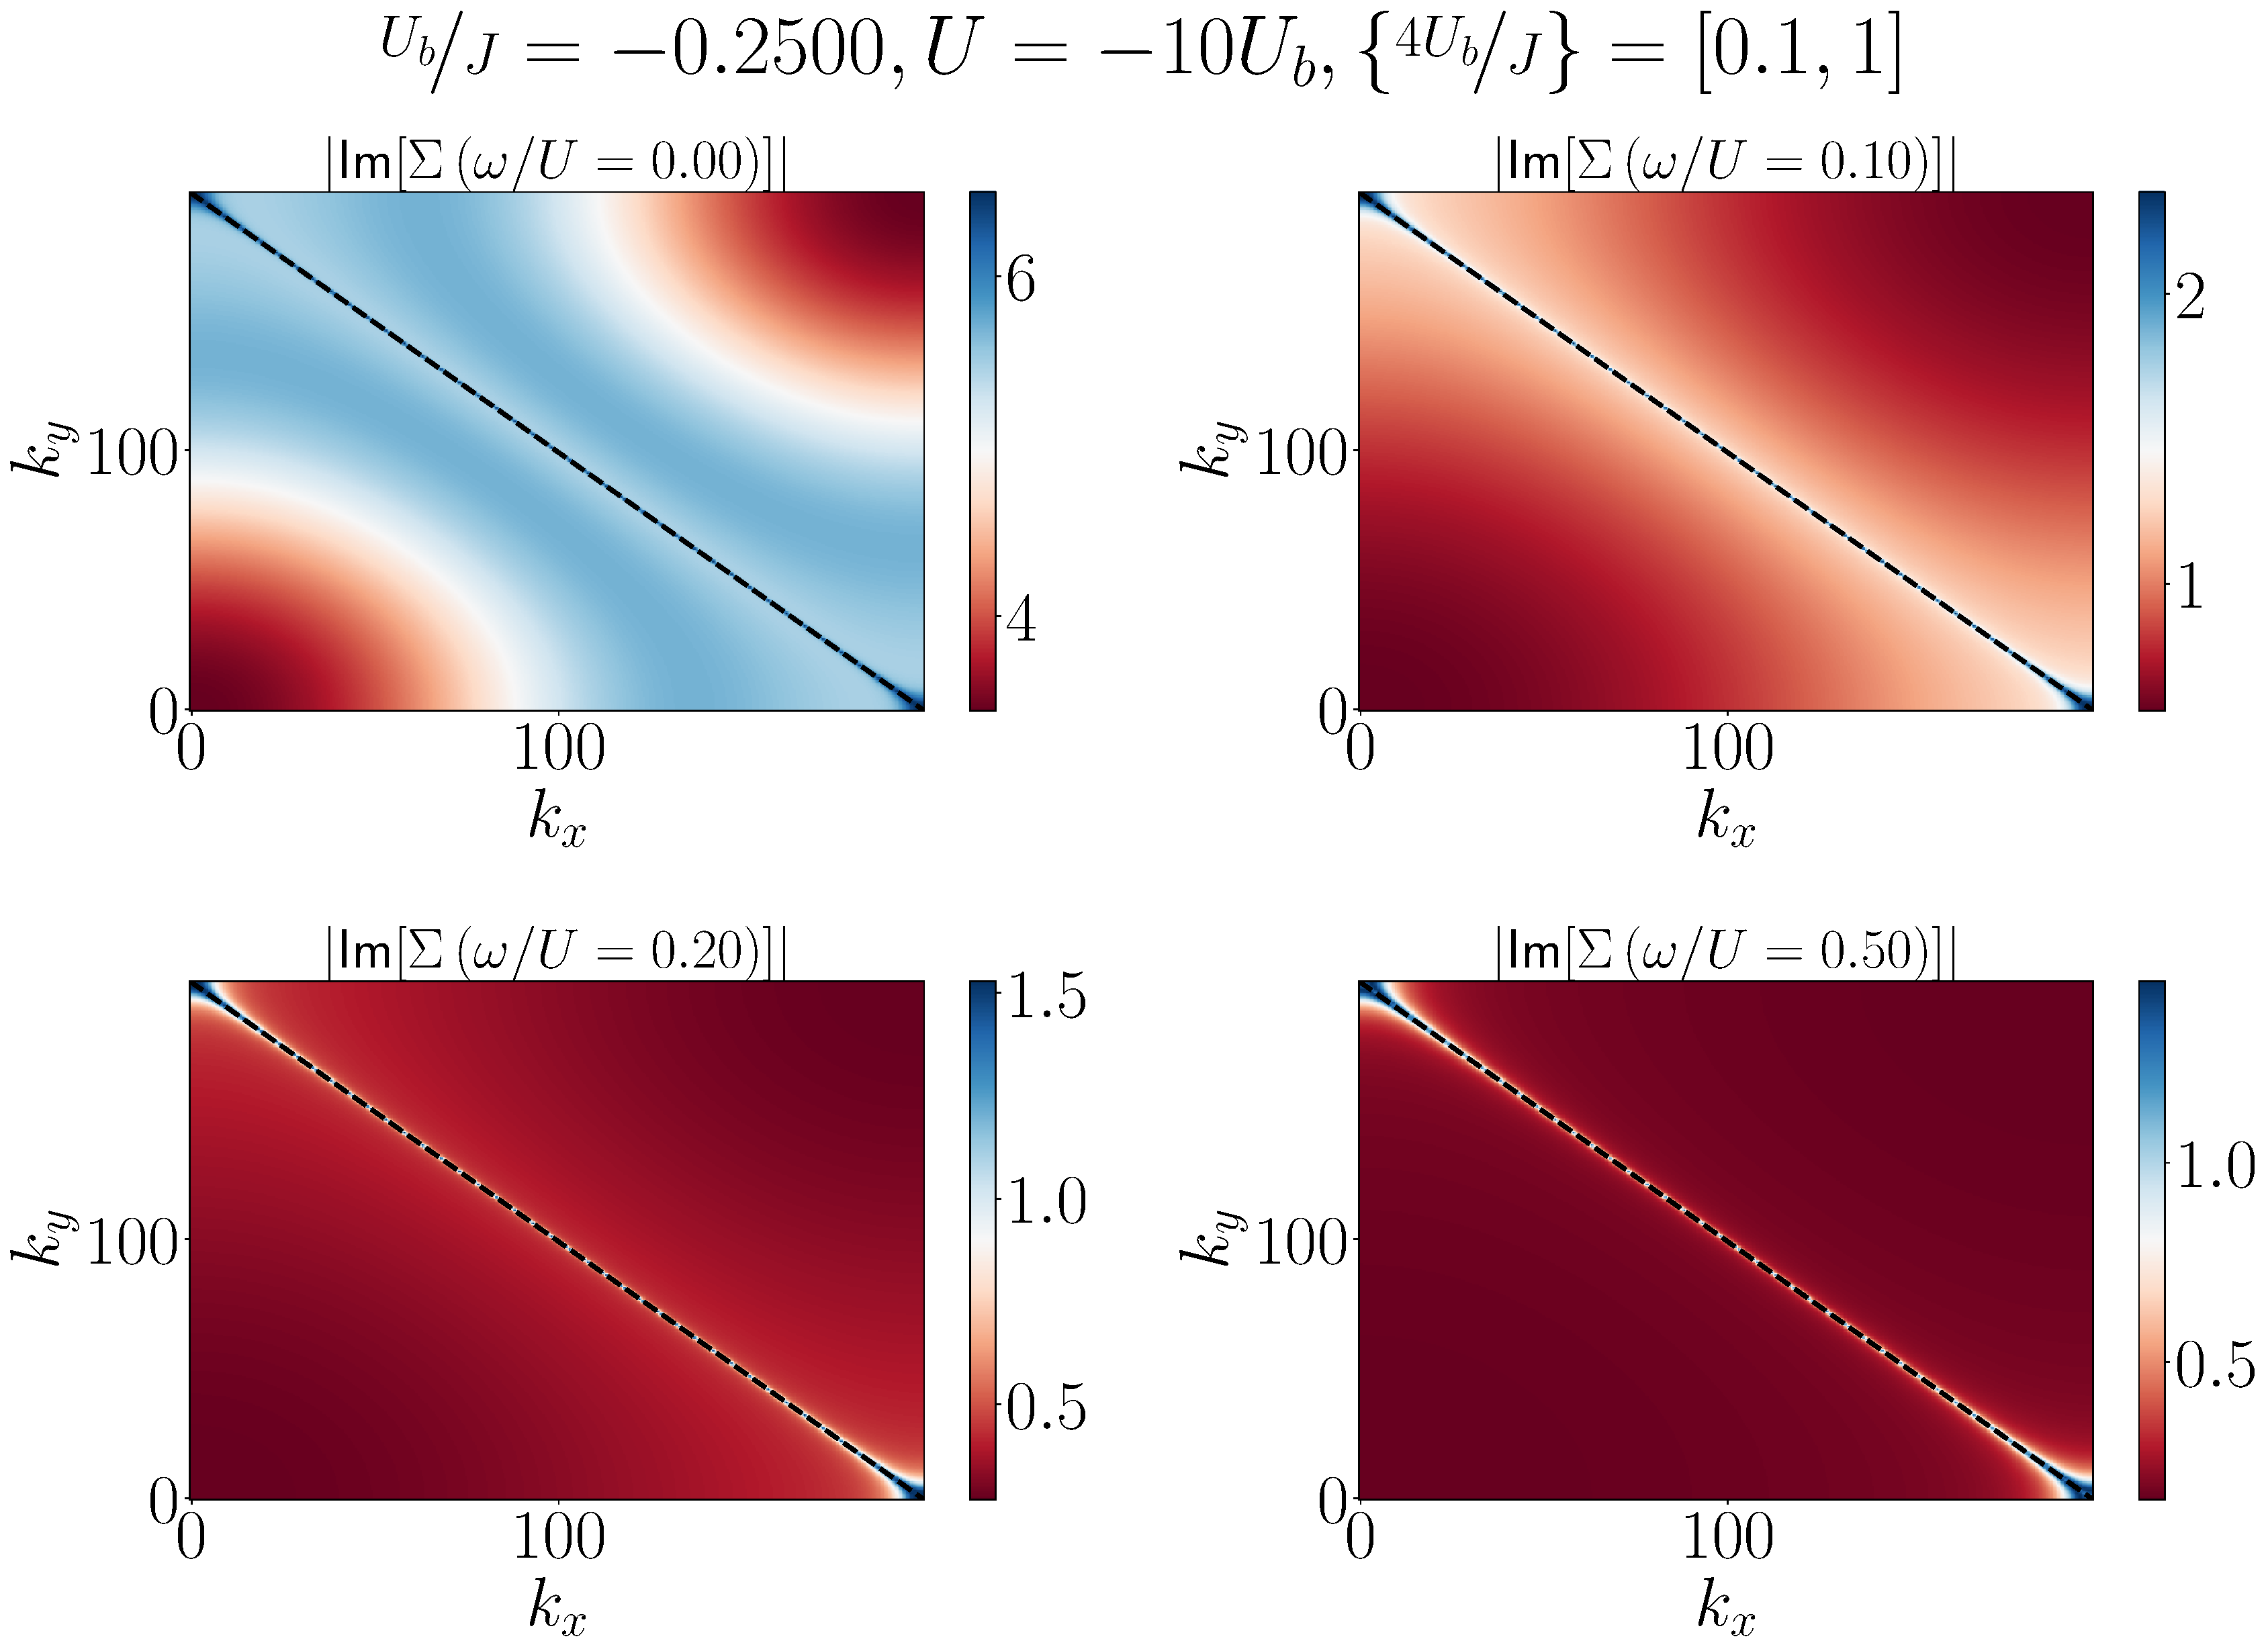
\includegraphics[height=0.3\textheight]{../figures/sigma-4-Ub_by_J=-0.25000-4.pdf} &
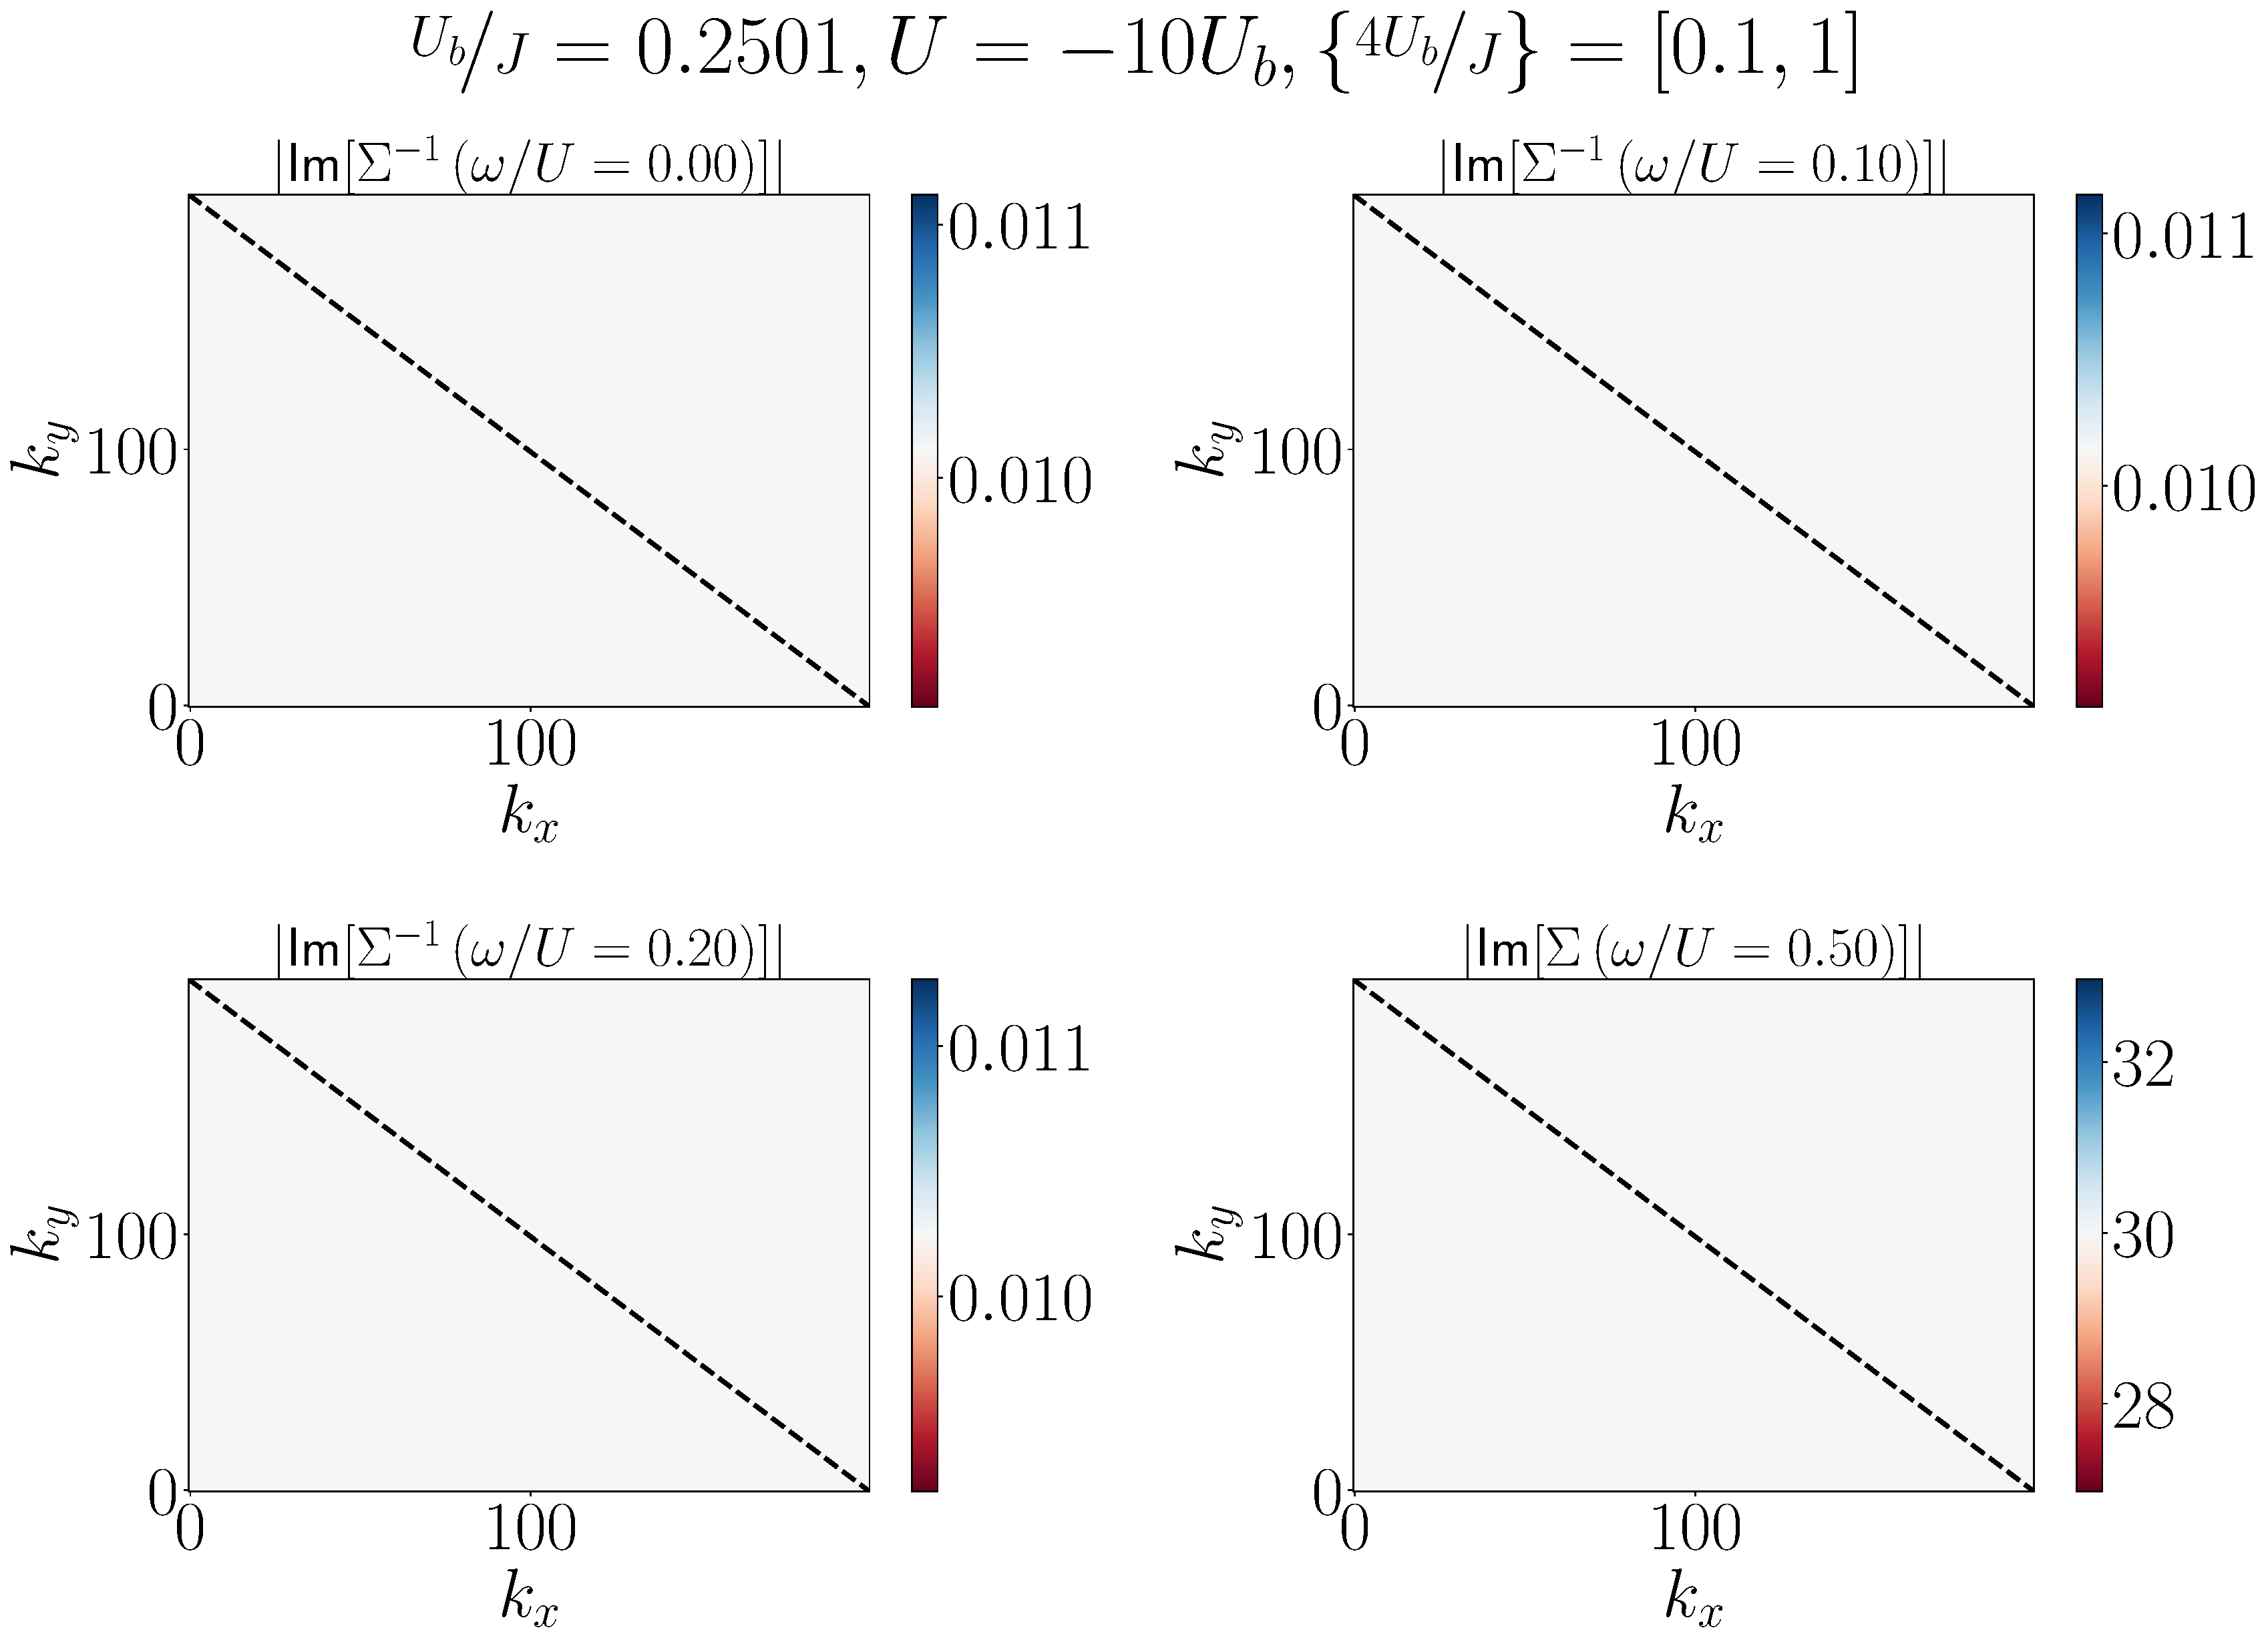
\includegraphics[height=0.3\textheight]{../figures/sigma-4-Ub_by_J=0.25010-4.pdf}
\end{tabular}
\captionof{figure}{Each of the 6 frames shows \(A(\vec k)\) at four values of \(\omega\). First 4 are before the transition (\(-U_b/J < 0.25\)), fifth is exactly at the transition \((-U_b/J = 0.25)\) and last one is after the transition (\(-U_b/J > 0.25\)). Available as video \href{https://abhirup-m.github.io/misc-sigma/}{\underline{here}}.}
\label{four-self}
\end{center}

In each frame, the top left figure represents the self-energy at \(\omega=0\). If we track this particular figure across the frames, we find that at small \(-U_b/J\), the self-energy near the Fermi surface was smaller than those near the Brillouin zone edges, indicating the presence of a prominent Fermi liquid. As \(U_b\) increases, we find that this distinction of the Fermi surface becomes less-prominent; at the critical point,we see that the self-energy near the Fermi surface self-energy has become more than that near the edges, signalling that the quasiparticle excitations have become scrambled because of the increased correlations in the bath.

If we, on the other hand, track the bottom right figure in each frame (\(\omega = U/2\)), we find that deep in the metallic regime, the self-energy is quite high. This is because of the low spectral weight at large \(\omega\). As the correlations are increased, we find that  this self-energy decreases, particular in comparison to the values at the Brillouin zone edges. This is because of the appearance of the Hubbard side-peaks in the local spectral function
.

In the insulating phase, we find that the momentum-dependence has vanished (the system is in the perfectly local atomic limit). The self-energy at the Hubbard side-bands (bottom right) is high, because the quasiparticle excitations are highly-renormalised and the single-particle picture description is not possible. The self-energy inside the gap (other three figures) diverges and the poles of the Greens function have been replaced by zeroes, so we have instead plotted the inverse self-energy.

These plots are available as videos \href{https://abhirup-m.github.io/misc-sigma/}{\underline{here}}.
}

\section{Some important remarks}
\subsection{Entanglement as an order parameter for the transition}
The spectral weights in the diagonal Greens function can be written in terms of a geometric measure of entanglement:
\begin{equation}\begin{aligned}
	d_n^p = \braket{\Phi_n | c^\dagger_{d\sigma} | \Phi_0} = \braket{\Phi_n | c^\dagger_{d\sigma} \sum_n \ket{\phi_m} \bra{\phi_m} | \Phi_0}
\end{aligned}\end{equation}
where, \(\ket{\phi_m}\) are the eigenstates of the Hamiltonian composed of a two-site system (formed by the impurity site and the zeroth site) in direct product with the rest of the lattice sites. The two site system interacts only via a spin-exchange coupling \(J\), and the impurity and bath sites have local correlations \(U\) and \(U_b\) respectively. The ground state is the spin-singlet in direct product with the ground state of the tight-binding chain formed by the remaining sites. The summation involves inner products of the ground state \(\ket{\Phi_0}\) with the eigenstates \(\ket{\phi_m}\). Only two states out of all \(\ket{\phi_m}\) give non-zero overlap - the spin singlet state \(\ket{SS}\) and the charge triplet-zero state \(\ket{CT}\). These two non-zero overlaps give rise to non-zero entanglement: \(\varepsilon_\text{SS} = 1 - |\braket{\Phi_0 | SS}|^2, \varepsilon_\text{CT} = 1 - |\braket{\Phi_0 | CT}|^2\). The spectral weight becomes
\begin{equation}\begin{aligned}
	d_n^p = \bra{\Phi_n} | c^\dagger_{d\sigma} \left(\ket{SS} + \ket{CT} \right) \left(\sqrt{1 - \varepsilon_\text{SS}} + \sqrt{1 - \varepsilon_\text{CT}}\right)
\end{aligned}\end{equation}
The total spectral weight can be written as
\begin{equation}\begin{aligned}
	|d_n^p|^2 = |\bra{\Phi_n} | c^\dagger_{d\sigma} \left(\ket{SS} + \ket{CT} \right)|^2 \left(2 - \varepsilon_\text{SS} - \varepsilon_\text{CT} + 2\sqrt{1 - \varepsilon_\text{SS}}\sqrt{1 - \varepsilon_\text{CT}}\right)
\end{aligned}\end{equation}
Near the metal, the ground state is, to a very good approximation, the state \(\ket{SS}\). One can then say that the entanglement \(\varepsilon_\text{SS}\) is poor - the entangled state is very close to the "separable" state. The term separable is used here in the sense that the metallic state defines a limit of the system. As \(U_b\) increases, \(\varepsilon_\text{SS}\) increases. On the other hand, the entanglement with the charge triplet is maximum in the metal, because the ground state does not have much of the charge triplet. Towards the MIT, this contribution increases, and the entanglement decreases.



\subsection{Topological nature of the transition}
As shown in section~\ref{lutt_theorem}, there is a difference in the value of the Luttinger volume between the local moment (LM) and the strong-coupling (SC) fixed points. If we define \(\mathcal{N}_L\) as the Luttinger volume with the spin-degeneracy accounted for, we can write
\begin{equation}\begin{aligned}
	\label{lutt_change}
	\mathcal{N}_L^\text{lm} - \mathcal{N}_L^\text{sc} = 1
\end{aligned}\end{equation}
where \(\mathcal{N}_L^\text{lm},\mathcal{N}_L^\text{sc}\) are the Luttinger volumes at the local moment and strong-coupling fixed points respectively. This equation expresses the fact that the Luttinger volume of the bath increases by \(1\) when the system is tuned from LM to SC, and this happens because the single-particle impurity excitation in the lower-Hubbard at the atomic limit gets transferred to the bath Greens function in the process. The quantity which tracks this transfer is therefore \(\mathcal{N}_\text{imp}\), the number of poles minus the number of zeros in the impurity Greens function at and below the Fermi surface:
\begin{equation}\begin{aligned}
	\label{imp_count_def}
	\mathcal{N}_\text{imp} = \begin{cases}
		1 & \text{ at LM}\\
		0 & \text{ at SC}
	\end{cases}\implies \Delta \mathcal{N}_\text{imp} = 1
\end{aligned}\end{equation}
The Luttinger volume \(\mathcal{N}_L\) is related to this impurity count by the equation
\begin{equation}\begin{aligned}
	\mathcal{N}_L = \mathcal{N} - \mathcal{N}_\text{imp}
\end{aligned}\end{equation}
where \(\mathcal{N}\) is the total number of electrons in the system, accounting for the spin degeneracy. If we keep this total number fixed (isolated system), the changes in the impurity count and Luttinger volume become constrained: 
\begin{equation}\begin{aligned}
	\Delta \mathcal{N}_L = - \Delta \mathcal{N}_\text{imp}~.
\end{aligned}\end{equation}
Eq.~\ref{imp_count_def} then readily implies eq.~\ref{lutt_change}.

In order to connect this impurity topological change with the bulk model, we write the total number of particles in the bulk system in the following manner:
\begin{equation}\begin{aligned}
	\mathcal{N} = \mathcal{N}_\text{loc} + \mathcal{N}_\text{deloc}
\end{aligned}\end{equation}
\(\mathcal{N}_\text{loc}\) is the number of real poles minus the number of zeros of the local Greens function. \(\mathcal{N}_\text{deloc}\) is the number of real poles minus the number of zeros of the \(k-\)space Greens functions. The former (latter) contributes only in the insulating (metallic) phase, because in the metallic (insulating) phase, the local (\(k-\)space) Greens function develop imaginary self-energy and the real poles in these Greens functions get replaced by imaginary poles. Together, these two terms accurately count the total number of particles in both these phases. These two terms are defined as
\begin{equation}\begin{aligned}
	\mathcal{N}_\text{loc} = \sum_i \mathcal{N}_i = \oint \frac{dz}{2\pi i}n_F(z) \text{Tr}\left[G_i(z)\right], ~ ~ ~\mathcal{N}_\text{deloc} = \sum_k \mathcal{N}_k = \oint \frac{dz}{2\pi i}n_F(z) \text{Tr}\left[G_k(z)\right] = \mathcal{N}_L
\end{aligned}\end{equation}
\(G_i(z)\) is the local Greens function at site \(i\) of the bulk model, and \(G_k(z)\) is the \(k-\)space Greens function in the bulk model. \(N_\text{deloc}\) is just the Luttinger volume \(\mathcal{N}_L\) of the bulk system. With this, the total number of particles in the bulk can be expressed as
\begin{equation}\begin{aligned}
	\label{bulk_total}
	\mathcal{N} = \sum_i \mathcal{N}_i + \mathcal{N}_\text{L}
\end{aligned}\end{equation}
From eq.~\ref{greens_func_siam}, we know that the bulk local Greens function is equal to that of the auxiliary model, and that gives \(\sum_i \mathcal{N}_i = \mathcal{N}_\text{imp}\sum_i = \mathcal{N} \mathcal{N}_\text{imp}\). There we used the fact that for a half-filled system, the total number of sites is equal to the total number of particles in the system. Substituting this into eq.~\ref{bulk_total} and again using \(\Delta \mathcal{N} = 0\) gives
\begin{equation}\begin{aligned}
	\mathcal{N} = \mathcal{N} \mathcal{N}_\text{imp} + \mathcal{N}_\text{L} \implies \Delta \mathcal{N}_\text{L} = - \mathcal{N} \Delta \mathcal{N}_\text{imp}
\end{aligned}\end{equation}
We already know that \(\Delta \mathcal{N}_\text{imp}=1\) across the transition, so we get
\begin{equation}\begin{aligned}
	\mathcal{N}_L^\text{metal} - \mathcal{N}_L^\text{insulator} = \mathcal{N}\left(\mathcal{N}_\text{imp}^\text{sc} - \mathcal{N}_\text{imp}^\text{lm}\right) = \mathcal{N}
\end{aligned}\end{equation}
The metal-insulator transition is therefore characterised by a change in the topological quantity \(\mathcal{N}_L\). The topological nature arises from the fact that it can be expressed in terms of winding numbers related to the corresponding Greens functions. \(\mathcal{N}_\text{imp}\), which derives from the impurity Greens function \(G_d\), is related to the winding numbers of the curves \(\text{Det}[G_d^{-1}(\Gamma^<)]\) and \(\text{Det}[G_d^{-1}(\Gamma^0)]\). The winding number is simply the number of times this function encircles the origin when traced on the curves \(\Gamma^<\) and \(\Gamma^0\) that enclose all poles inside and on the Fermi surface respectively. An example of such a winding number is shown in fig.~\ref{imp_winding}.
\begin{figure}[!htb]
	\centering
	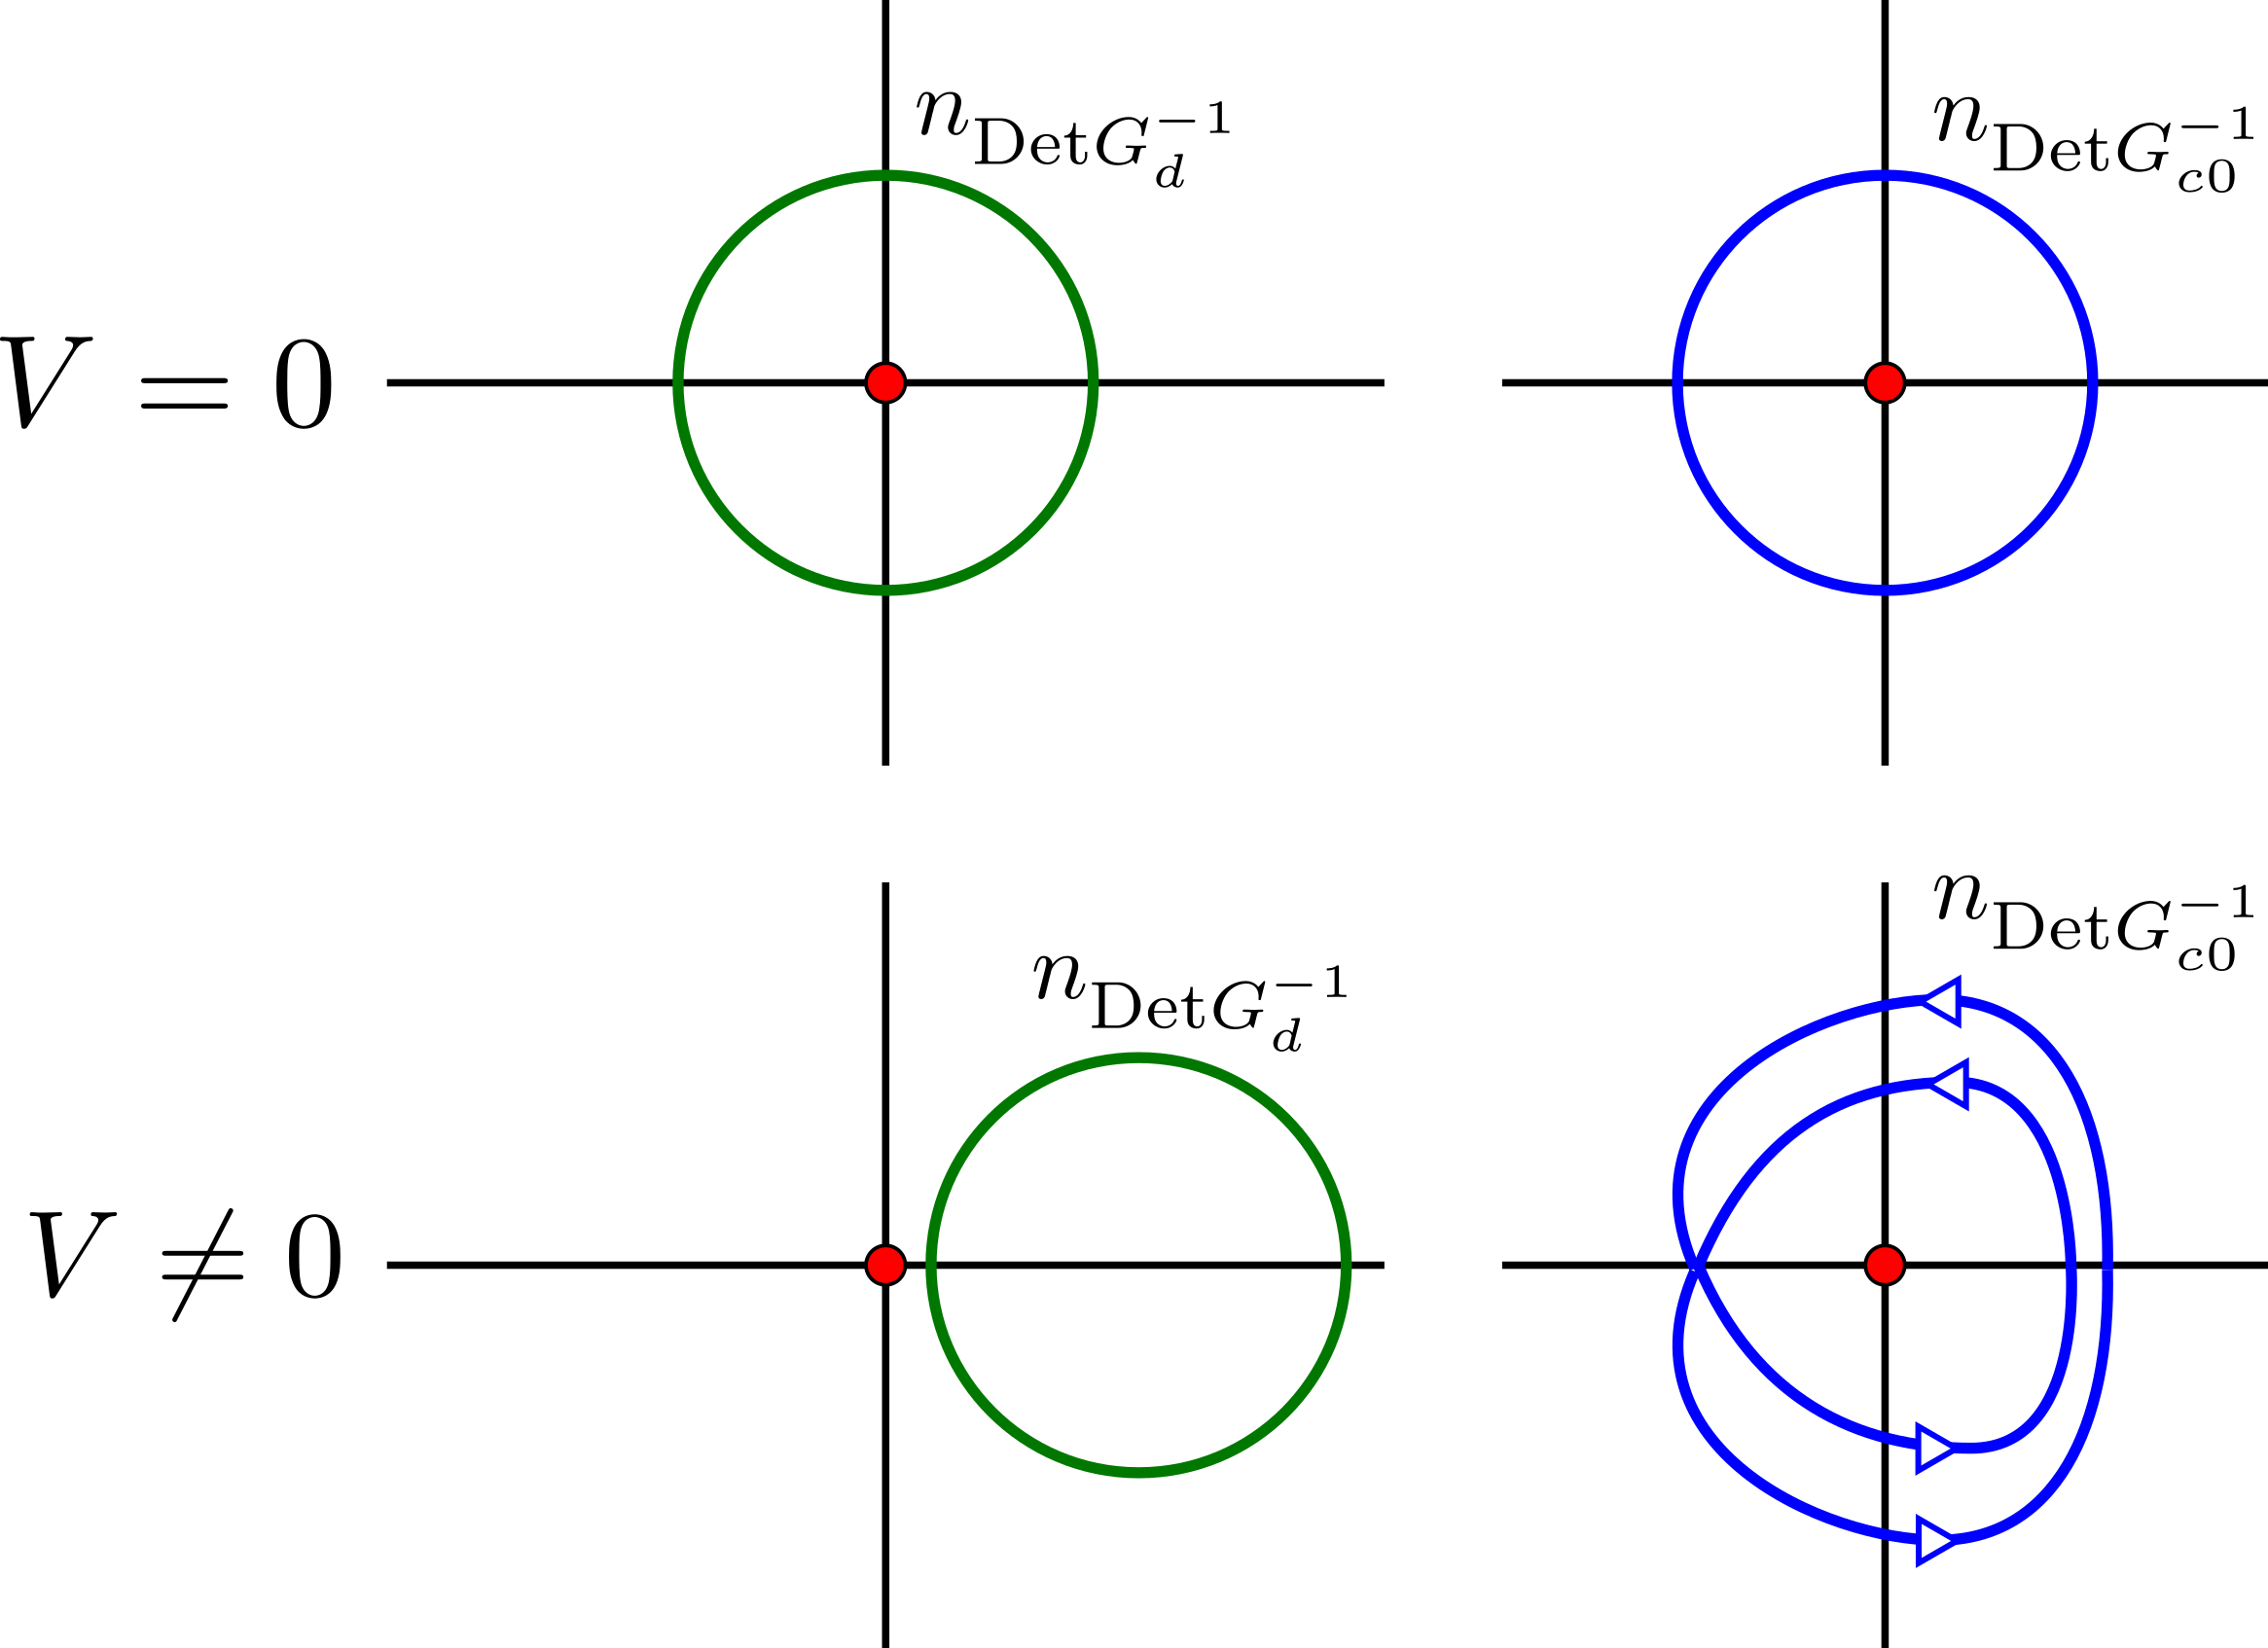
\includegraphics[scale=0.2]{../figures/luttinger_top_change.png}
	\caption{The green lines describe the winding number related to the impurity Greens function, while the blue lines do it for the bath. At the local moment fixed point \(V=0\), the impurity has a winding number of 1 because the curve encircles the origin once. At the strong-coupling fixed point, this winding number becomes zero, indicated by the fact that the curve does not encircle the origin even once. The reduction in the winding number on the part of the impurity is directly linked to the increase in the winding number of the bath - it encircles the origin once at the local moment fixed point but twice at strong-coupling.}
	\label{imp_winding}
\end{figure}


\subsection{Greens function in the insulating phase: the Hubbard bands and mottness}
In the insulating state, the cluster becomes a local moment and the bulk system reduces to the atomic limit \(H = -\frac{U}{2}\sum_i\left(\hat n_{i \uparrow} - \hat n_{i \downarrow}\right)^2\). The Greens function in this limit is given in Appendix~\ref{atomic limit}. From eq.~\ref{atomic_limit_gf}, we have
\begin{equation}\begin{aligned}
	G_{i}(\omega) = \sum_\sigma G_{i,\sigma}(\omega) = \frac{1 + \left<\tau_{i }\right>}{\omega - \frac{U}{2}} + \frac{1 - \left<\tau_{i}\right>}{\omega + \frac{U}{2}}
\end{aligned}\end{equation}
where \(\tau_i = \sum_\sigma \hat n_{i,\sigma} - 1\). At half-filling \(\left<\tau_{i}\right>=0\), the low and high-energy poles have equal spectral weights. \textit{This is different from the situation in a band insulator, where the valence band has all the spectral weight in the ground state while the conduction band is empty.} On doping holes into the system such that \(\left<\tau_{i}\right> = -x < 0\), spectral weight is transferred from the upper Hubbard band at \(\omega = U/2\) to the lower one at \(\omega = -U/2\):

\begin{equation}\begin{aligned}
	G_{i}(\omega) = \sum_\sigma G_{i,\sigma}(\omega) = \frac{1 - x}{\omega - \frac{U}{2}} + \frac{1 + x}{\omega + \frac{U}{2}}
\end{aligned}\end{equation}
\textit{This transfer of spectral weight across energy scales of the order of \(U\), as well as the lack of poles at zero energies, is referred to as mottness}~\cite{phillips2006mottness}.
\begin{figure}[!htb]
	\centering
	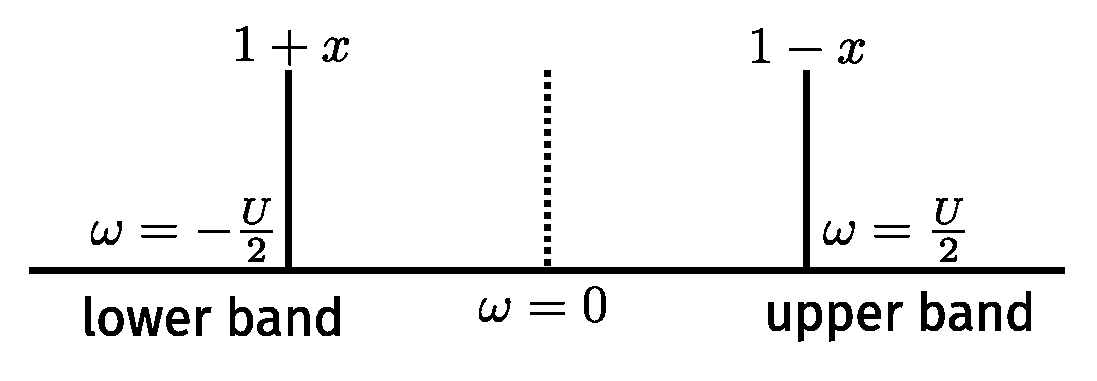
\includegraphics[width=0.5\textwidth]{../figures/hubbard_bands.pdf}
	\caption{Structure of the Greens function in the atomic limit. The two poles at \(\omega = \pm \frac{U}{2}\) form the two Hubbard bands. Doping the system leads to transfer of spectral weight between the bands.}
\end{figure}

\subsection{Nature of propagation: metal vs insulator}
In the metallic state, the impurity in the auxiliary model hybridises with the bath through both 1-particle and 2-particle interactions. For any two auxiliary models differing by the locations \(i_1, i_2\) of the impurity, the baths will always overlap. This means that an electron that starts out from the impurity site at \(i_1\) can hop into the bath, and eventually reach \(i_2\) by hopping out of the other bath and into the other impurity. Such processes connect all sites of the lattice and \textit{allow spectral flow}.

In the insulating state, each auxiliary model separates into an impurity and a bath that decoupled from each other. This means that the impurity cannot hybridise into the bath, and hence cannot tunnel into any other impurity. This leads to the atomic limit of the system, where each site develops a local moment configuration because of the repulsive local correlation, but these local moments cannot communicate with each other, either through spin-exchange processes or by breaking into holons and doublons. Any attempt at spectral flow fails because the boundaries of the system become disconnected from each other.

A more accurate picture of the insulating and metallic phases can be obtained by working with a more complicated choice of the cluster. For instance, instead of a single impurity, one can take two correlated impurities interacting with each other through a single-particle hopping, and this cluster then interacts with the bath through the usual interactions. The ground state of such a cluster is actually a quantum liquid, consisting of the entangled spin and charge degrees of freedom. In the metallic state, various members of this liquid such as the holons, doublons and the spinons are free to propagate across the system through the baths. In the insulating state, it is this cluster that then gets decoupled from the other clusters. The composite degrees of freedom are then unable to propagate outside the cluster, and \textit{the holons and the doublons are bound to each other}~\cite{Mott_1949} within the confines of the cluster.

\begin{figure}[ht]
	\centering
	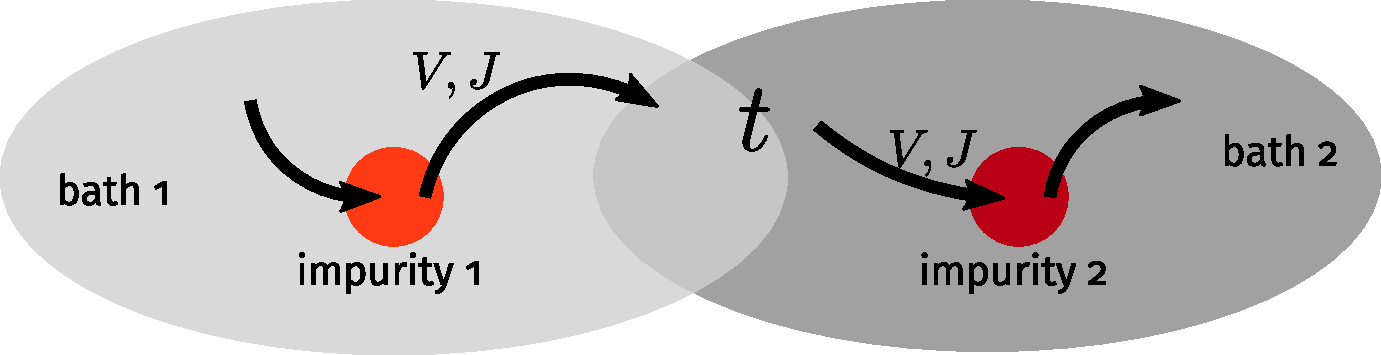
\includegraphics[width=0.55\textwidth]{../figures/metal_prop.pdf}
	\caption{Propagation of electrons from one cluster to another through the bath, in the metallic state}
\end{figure}

\begin{figure}[!ht]
	\centering
	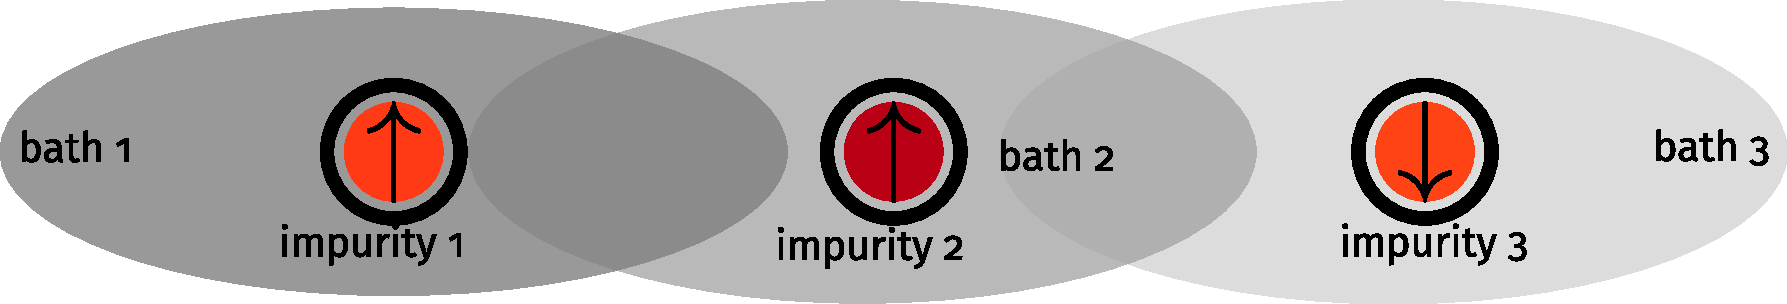
\includegraphics[width=0.75\textwidth]{../figures/ins_prop.pdf}
	\caption{The clusters get isolated from each other in the insulator, because they get decoupled from their baths.}
\end{figure}

\begin{figure}[!ht]
	\centering
	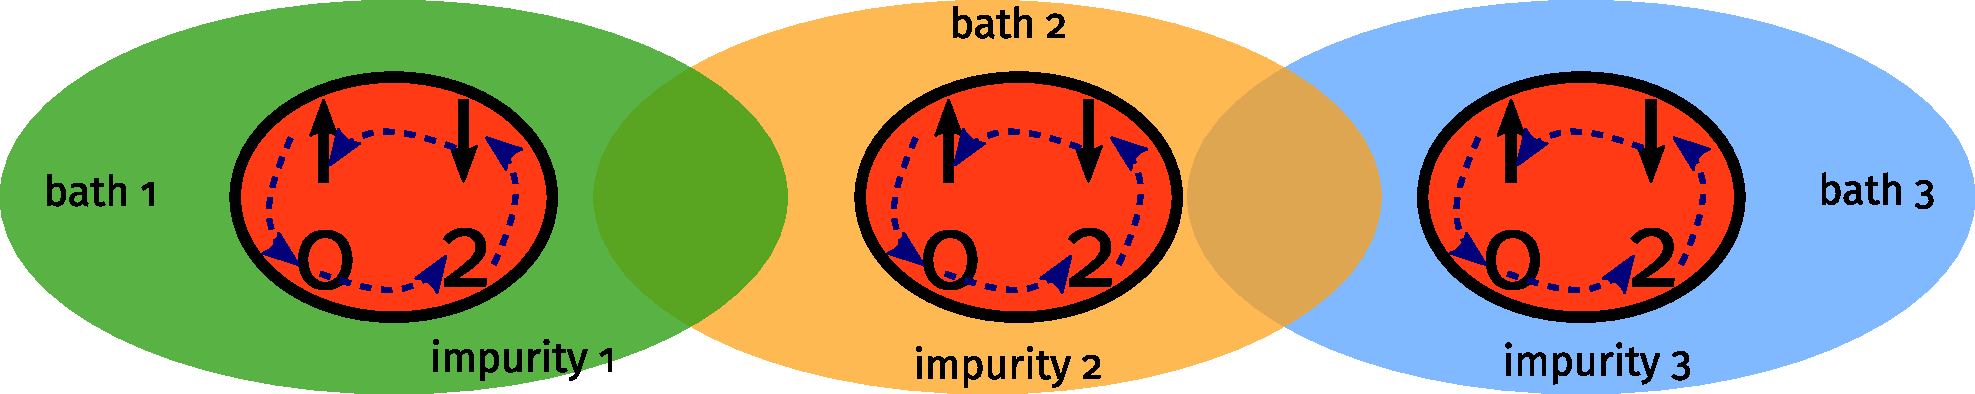
\includegraphics[width=0.85\textwidth]{../figures/ins_prop_cluster.pdf}
	\caption{Each cluster is a quantum liquid composed of spin \(\left(\uparrow,\downarrow\right) \) and charge \(\left(0,2\right) \) degrees of freedom. In the insulating state, these degrees of freedom get bound within the cluster and are unable to propagate outside.}
\end{figure}

\subsection{Presence of two self-energies under symmetry-breaking}
The effective Hamiltonian that describes either the metallic or the insulating phase has $\mathrm{SU}(2)$ symmetry in both the spin and charge sectors. Since the repulsive correlation on the impurity picks out the spin sector, we focus on that for now. Applying a small magnetic field on the impurity breaks this spin-rotation symmetry and picks out either the up or the down state on the impurity, leading to two kinds of self-energies, one for each spin state~\cite{logan_2014,Logan_2015}. The Hamiltonian has the form \(H(h)_i = -\frac{U}{2}\left(\hat n_{i \uparrow} - \hat n_{i \downarrow}\right)^2 - h\left(\hat n_{i \uparrow} - \hat n_{i \downarrow}\right)\). The unique groundstate is \(\ket{\hat n_{i,\sigma = \text{sgn}(h)}=1,\hat n_{i,\sigma = -\text{sgn}(h)}=0}\), with an energy of \(E_\text{gs} = -\frac{U}{2} - h\). The Greens function is easiest to obtain from the Lehmann-Kallen representation (eq.~\ref{Gf_lk}):
\begin{equation}\begin{aligned}
	G_{i,\sigma} = \sum_{n}\left[||\bra{\text{GS}}c_{i\sigma}\ket{n}||^2\frac{1}{\omega + E_\text{GS} - E_n} + ||\bra{n}c_{i\sigma}\ket{\text{GS}}||^2\frac{1}{\omega - E_\text{GS} + E_n}\right]\\
\end{aligned}\end{equation}
We have \(c_{i,\sigma}\ket{\text{GS}} = \ket{\hat n_i = 0}\delta_{\sigma,\text{sgn}(h)}\) and \(c^\dagger_{i,\sigma}\ket{\text{GS}} = \ket{\hat n_i = 2}\delta_{\sigma,-\text{sgn}(h)}\), so that the only excited states that give non-zero inner product is \(\ket{n}=\ket{\hat n_i = 0}\) for the second term and \(\ket{n}=\ket{\hat n_i=2}\) for the first term, with energies \(E_n=0\). Substituting these, we get
\begin{equation}\begin{aligned}
	G_{i,\sigma}(h) = \frac{\delta_{\sigma,-\text{sgn}(h)}}{\omega - \frac{U}{2} - h} + \frac{\delta_{\sigma,\text{sgn}(h)}}{\omega + \frac{U}{2} + h} = \frac{1}{\omega + \left(\frac{U}{2}+h\right)\sigma \times \text{sgn}(h) }
\end{aligned}\end{equation}
Taking the limit of \(h \to 0^\pm\) then gives
\begin{equation}\begin{aligned}
	G_{i,\sigma}(h=0^\pm) = \frac{1}{\omega \pm \frac{U}{2}\sigma}
\end{aligned}\end{equation}
The self-energies arising from the correlation \(U\) can also be obtained using Dyson's equation \(\Sigma = G^{-1} - G_0^{-1}\), where \(G_0^{-1} = \omega\) is the Greens function at \(U=0\). Using Dyson's equation, we get
\begin{equation}\begin{aligned}
	\Sigma_{i,\sigma} = \pm\frac{U}{2}\sigma
\end{aligned}\end{equation}

\section{Analytic consistency check - On the Bethe lattice}
One can apply a test to this method: it involves considering the case of infinite number of nearest-neighbours $w\to\infty$ (the coordination number, and effectively the dimension). In such a model, the correct scaling of the $t^{H}$ hopping parameter is $t^{H}\to t^{H}/\sqrt{w}$~\cite{metzner_volhardt_1989,georges_kotliar_1992,pruschke_cox_jarrel_1993}, such that the kinetic energy of the associated tight-binding lattice model remains finite and in competition with the localising physics of \(U\) and the magnetic ordering physics of \(J\). This allows a metal-insulator transition in the limit of $w\to\infty$ as well. In this limit, the dependence of the self-energy on the interacting Greens functin can be shown to arise from only the site-diagonal terms~\cite{Muller-Hartmann1989,georges_kotliar_1992}. This can be demonstrated from the present formalism as well, using eq.\eqref{self-energy1}. Applying the limit of \(w\to \infty\) on that equation gives
\begin{equation}\begin{aligned}
	\Sigma_{H-H}(\vec k,\omega) = \lim_{w\to \infty} \left\{\left(G^{(0)}(\vec k,\omega)\right)^{-1} - \left [G_\text{aux,dd} + \frac{\xi_{\vec k}}{w} G_\text{aux,dz}\right]^{-1}\right\} = \lim_{w\to \infty}\left\{G^{(0)}(\vec k,\omega) - G_\text{aux,dd}(\omega)\right\}^{-1} 
\end{aligned}\end{equation}
where \(G^{(0)}(\vec k,\omega)\) is the non-interacting Greens function and \(G_\text{aux,dd}(\omega)\) is the site-diagonal Greens function of the auxiliary model. It is clear from the final form that only the diagonal term \(G_\text{aux,dd}(\omega)\) of the interacting Greens function affects the self-energy while the off-diagonal part \(G_\text{aux,dz}\) fails to contribute as \(w \to \infty\). Even the non-interacting part Greens function can be shown to be diagonal in the limit of \(w\to\infty\)~\cite{kuramoto_manybody}. From its definition in time domain, we have
\begin{equation}\begin{aligned}
	G^{(0)}(\vec k, t) = -i\theta(t) \left<\left\{c_{\vec k}(t), c^\dagger_{\vec k}\right\} \right> = -i\theta(t) \left<\left\{e^{i H^{(0)}t} c_{\vec k} e^{-i H^{(0)}t}, c^\dagger_{\vec k}\right\} \right> = -i\theta(t) e^{-i \epsilon_{\vec k}t}\left[ \left<1 - \hat n_{\vec k}\right> + \left<\hat n_{\vec k}\right>\right] = -i \theta(t) e^{-i \epsilon_{\vec k}t}
\end{aligned}\end{equation}
A quick Fourier transform to \(\omega-\)domain shows that this is identical to the \(G^{(0)}(\vec k, \omega)\) defined just above eq.~\ref{self-energy}. We note that \(|G^{(0)}(\vec k, t)| \leq 1\). Using the Fourier transform  definition
\begin{equation}\begin{aligned}
	f(\vec k) = \frac{1}{d_N}\sum_{\vec r_i}h(\vec r_i) e^{i \vec{k}\cdot\vec{r}_i}
\end{aligned}\end{equation}
where \(d_N\) is a factor that only depends on the total number of sites and not on the coordination number, we can write
\begin{equation}\begin{aligned}
	|G^{(0)}(\vec k, t)|^2 = \frac{1}{d_N^2}\sum_{\vec r_i, \vec r_j} G^{(0)}(\vec r_i, t)\left(G^{(0)}(\vec r_j, t)\right)^* e^{i \vec k \cdot \left(\vec r_i - \vec r_j\right) t}
\end{aligned}\end{equation}
From the inequality \(|G^{(0)}(\vec k, t)| \leq 1\), we get
\begin{equation}\begin{aligned}
	1 \geq \frac{1}{N}\sum_k |G^{(0)}(\vec k, t)|^2 = \frac{1}{N d_N^2}\sum_{\vec r_i, \vec r_j} G^{(0)}(\vec r_i, t)\left(G^{(0)}(\vec r_j, t)\right)^* \underbrace{\sum_k e^{i \vec k \cdot \left(\vec r_i - \vec r_j\right) t}}_{N \delta_{\vec r_i = \vec r_j}} = \frac{1}{d_N^2}\sum_{\vec r_i} |G^{(0)}(\vec r_i, t)|^2
\end{aligned}\end{equation}
For a coordination number of \(w\), there are \(w\) number of \(\vec r_i\) that are equivalent: \(\sum_{\vec r_i \in \text{NN}}|G^{(0)}(\vec r_i, t)|^2\). Adding these equal Greens functions and ignoring the \(w-\)independent prefactor in front, we obtain \(|G^{(0)}(\vec r_i, t)|^2 \sim \frac{1}{w}\). In contrast, there is only one local Greens function, that for \(\vec r_i=0\). The local Greens function therefore scales independent of \(w\). This implies that 
\begin{equation}\begin{aligned}
	\lim_{w\to \infty}G^{(0)}(\vec k,\omega) = G^{(0)}(\vec r=0,\omega)
\end{aligned}\end{equation}
Since both the non-interacting and the interaction Greens functions lose their non-locality, the self-energy becomes completely local in the limit of \(w \to \infty\).

\chapter{Going to larger clusters - the two site approach}

\section{Why expand the cluster?}
The previous chapter dealt with treating the Hubbard-Heisenberg model using an auxiliary model that has a single-site cluster:
\begin{equation}\begin{aligned}
	\mathcal{H}_\text{aux} =  \sum_{k\sigma}\epsilon_k \tau_{k\sigma} - \frac{U}{2}\left( \hat n_{d \uparrow} - \hat n_{d \downarrow} \right) ^2 + \sum_{k\sigma} \left(V_{k} c^\dagger_{k\sigma} c_{d\sigma} + h.c.\right) +J \vec{S_d}\cdot\vec{s}_0 - U_b\left(\hat n_{0 \uparrow} - \hat n_{0 \downarrow}\right)^2
\end{aligned}\end{equation}
This was able to describe an impurity phase transition from screened strong-coupling phase to local moment weak coupling phase, upon tuning \(U_b/J\). This then leads to a metal-insulator transition in the bulk, owing to the relations between the Greens functions and spectral functions obtained earlier. The single-site nature of the cluster (there was only a single impurity) has the following consequences:
\begin{itemize}
	\item [1.] The \(k-\)space self-energy of the bath has only minimal \(k-\)dependence arising from nearest-neighbour non-locality between the impurity and the zeroth site of the bath.
	\item [2.] The local moment phase (which reduces to a set of decoupled clusters) becomes just the atomic limit, because each cluster has just one impurity.
\end{itemize}

In this chapter, we will improve on these two points by considering a larger cluster that has two impurities interacting with each other:
\begin{equation}\begin{aligned}
	\label{dimer_ham}
	H_\text{aux} = \sum_{i=1,2} \left[- \frac{U}{2}\left(\hat n_{d_i \uparrow} - \hat n_{d_i \downarrow}\right)^2 + V\sum_{\sigma}\left(c^\dagger_{d_i\sigma}c_{0_i\sigma} + \text{h.c.}\right) + J \vec{S}_{d_i}\cdot\vec{s}_{0_i} - U_b\left(\hat n_{0_i \uparrow} - \hat n_{0_i \downarrow}\right)^2\right]\\
	 -t \sum_\sigma \left(c^\dagger_{d_1,\sigma}c_{d_2,\sigma} + \text{h.c.}\right) + \sum_{k\sigma}\epsilon_k \tau_{k\sigma}
\end{aligned}\end{equation}
\(d_1\) and \(d_2\), or \(d_i\) in general, represent the two impurity sites in the dimer. They interact with each other through the same hopping parameter \(t\) as the bath. Each of the impurities has its own correlation \(U\) and hybridisation with the bath through \(V\) and \(J\). Each impurity site \(d_i\) couples with a bath site \(0_i\). \(0_1\) and \(0_2\) are assumed to be adjacent to each other, connected by the hopping \(t\). The setup is shown in fig.~\ref{two-imp-cluster}.

Note that this chapter only sets out the relations between such an auxiliary model and the corresponding bulk model (in this case, a Hubbard-Heisenberg), but does not describe the physics of this new auxiliary model. That requires performing a renormalisation group calculation for \(H_\text{aux}\), and that will be provided at a later point in time.

\begin{figure}[!htb]
	\centering
	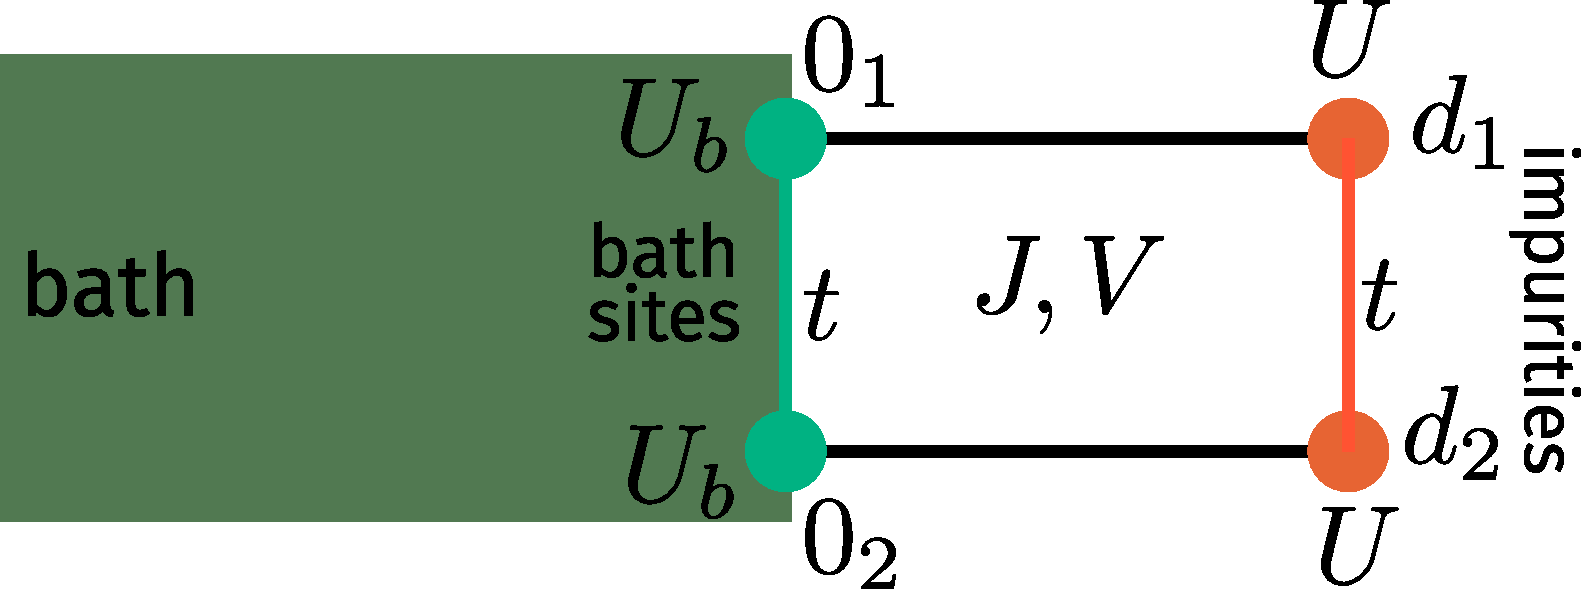
\includegraphics[width=0.6\textwidth]{../figures/two-site-cluster.pdf}
	\caption{Two-impurity SIAM hybridising with a bath}
	\label{two-imp-cluster}
\end{figure}

\section{Solution of the Hubbard dimer using the Anderson molecule}
This section tries to see how far we can we can go if we just work with the Anderson molecule as the smallest unit of tiling. We will attempt to reproduce the entire spectrum of a Hubbard dimer by creating a new Hamiltonian made up purely of Anderson molecules. This will guide us in deciding how to generalize the "tiling method" for a general $N-$site Hubbard model, as well as give indications as to whether we need a different smallest unit for tiling.

The Hubbard dimer and Anderson molecules (zero-mode) are defined by the following respective Hamiltonians:
\begin{equation}\begin{aligned}
	H^H &= -t^H\sum_{\sigma}\left(c^\dagger_{1\sigma}c_{2\sigma} + \text{h.c.}\right) + U^H\sum_{i=1,2}\hat n_{i \uparrow}\hat n_{i \downarrow} - \mu^H \sum_{\sigma, i=1,2}\hat n_{i\sigma}\\
	H^A &= -t^A\sum_{\sigma}\left(c^\dagger_{d\sigma}c_{z\sigma} + \text{h.c.}\right) + \epsilon_d^A \sum_{\sigma}\hat n_{d\sigma} + U^A\hat n_{d \uparrow}\hat n_{d \downarrow}
\end{aligned}\end{equation}
In the first Hamiltonian, the indices \(i=1,2\) refer to the two lattice sites that constitute the dimer. In the second Hamiltonian, the subscript \(d\) indicates the impurity site, while the subscript \(z\) indicates the zero-mode site. First, we will assume that the Hubbard dimer is at half-filling (\(\frac{1}{2}U^H = \mu^H\)):
\begin{equation}\begin{aligned}
	\label{hubb_dimer}
	H^H &= -t^H\sum_{\sigma}\left(c^\dagger_{1\sigma}c_{2\sigma} + \text{h.c.}\right) + U^H\sum_{i=1,2}\hat \tau_{i \uparrow}\hat \tau_{i \downarrow} + \left(\frac{1}{2}U^H- \mu^H\right) \sum_{\sigma, i=1,2}\hat n_{i\sigma} + \text{constant}\\
	    &= -t^H\sum_{\sigma}\left(c^\dagger_{1\sigma}c_{2\sigma} + \text{h.c.}\right) + U^H\sum_{i=1,2}\hat \tau_{i \uparrow}\hat \tau_{i \downarrow}
\end{aligned}\end{equation}
Since the Hubbard Hamiltonian is at half-filling, we will also place the impurity at half-filling by setting \(\epsilon_d^A = -\frac{1}{2}U^A\):
\begin{equation}\begin{aligned}
	\label{and_dimer}
	H^A &= -t^A\sum_{\sigma}\left(c^\dagger_{d\sigma}c_{z\sigma} + \text{h.c.}\right) + \left(\epsilon_d^A + \frac{1}{2}U^A\right) \sum_{\sigma}\hat \tau_{d\sigma} + U^A\hat \tau_{d \uparrow}\hat \tau_{d \downarrow} + \text{constant}\\
	    &= -t^A\sum_{\sigma}\left(c^\dagger_{d\sigma}c_{z\sigma} + \text{h.c.}\right) + U^A\hat \tau_{d \uparrow}\hat \tau_{d \downarrow}
\end{aligned}\end{equation}
The first step is to recreate the Hubbard dimer Hamiltonian eq.~\ref{hubb_dimer} using the Anderson molecule Hamiltonian eq.~\ref{and_dimer}:
\begin{equation}\begin{aligned}
	H^H &= -t^H\sum_{\sigma}\left(c^\dagger_{1\sigma}c_{2\sigma} + \text{h.c.}\right) + U^H\sum_{i=1,2}\hat \tau_{i \uparrow}\hat \tau_{i \downarrow}\\
	    &= \frac{1}{2}\left[-t^H\sum_{\sigma}\left(c^\dagger_{1\sigma}c_{2\sigma} + \text{h.c.}\right) + t^H\sum_{\sigma}\left(c^\dagger_{2\sigma}c_{1\sigma} + \text{h.c.}\right)\right] + \frac{1}{2} 2U^H\sum_{i=1,2}\hat \tau_{i \uparrow}\hat \tau_{i \downarrow}\\
	    &= \frac{1}{2}\left[-t^A\sum_{\sigma}\left(c^\dagger_{d\sigma}c_{z\sigma} + \text{h.c.}\right)\bigg\vert_{z \to 2, d \to 1\atop{t^A \to t^H}} + t^A\sum_{\sigma}\left(c^\dagger_{2\sigma}c_{1\sigma} + \text{h.c.}\right)\bigg\vert_{d \to 2,z \to 1\atop{t^A \to t^H}} \right] \\
	    &+ \frac{1}{2} \left(U^A\hat \tau_{i \uparrow}\hat \tau_{i \downarrow}\bigg\vert_{d \to 1\atop{U^A \to 2U^H}} + U^A\hat \tau_{i \uparrow}\hat \tau_{i \downarrow}\bigg\vert_{d \to 2\atop{U^A \to 2U^H}}\right)\\
	    &=\frac{1}{2}\left[H^A\left(t^A \to t^H, U^A \to 2U^H, d \to 1, z \to 2\right) + H^A\left(t^A \to t^H, U^A \to 2U^H, d \to 2, z \to 1\right)\right]
\end{aligned}\end{equation}
The conclusion we can draw from this is that the Hubbard dimer Hamiltonian can be obtained from the Anderson dimer Hamiltonian in the following fashion:
\begin{itemize}
	\item The essential idea is that we have to create a local Hubbard Hamiltonian for each site of the Hubbard lattice by replacing the impurity label \(d\) in the Anderson dimer with the label of the particular site. So if there are two sites, we will get two local Hamiltonians obtained by replacing \(d\) with 1 and 2 respectively. For each local Hamiltonian, the zero-mode label \(z\) is replaced by the site that is nearest to the one that \(d\) is being replaced by. So, if \(d \to 1(2)\), then \(z \to 2(1)\).
	\item This, however, is not the only change that we must make, in order to get the local Hamiltonian for a particular site. Along with \(d\) and \(z\), we must also make the transformations \(t^A \to t^H, U^A \to 2U^H\).
	\item Finally, once we have the local Hamiltonians for sites 1 and 2, we average them to get the total Hubbard Hamiltonian.
\end{itemize}
Note that we expect most of these "rules" to be specific for the dimer, and there will be generalizations to most of them for a general \(N-\)site Hubbard Hamiltonian.


The wavefunctions for the \(N=2\) sector can also be connected through these transformations. Since both the Hamiltonians are analytically solvable, we can write down their groundstate wavefunctions [CITE PAVARINI]:
\begin{equation}\begin{aligned}
	\ket{\Psi^H_\text{GS}} &= a_1(U^H, t^H)\frac{1}{\sqrt 2}\left(\ket{\uparrow_1, \downarrow_2} - \ket{\downarrow_1, \uparrow_2}\right) - a_2(U^H,t^H){\sqrt 2}\left(\ket{\uparrow_1\downarrow_1, } - \ket{,\uparrow_2\downarrow_2}\right)\\
	\ket{\Psi^A_\text{GS}} &= a_1(\frac{1}{2}U^A, t^A)\frac{1}{\sqrt 2}\left(\ket{\uparrow_d, \downarrow_z} - \ket{\downarrow_d, \uparrow_z}\right) - a_2(\frac{1}{2}U^A,t^A){\sqrt 2}\left(\ket{\uparrow_d\downarrow_d, } - \ket{,\uparrow_z\downarrow_z}\right)\\
	E^H_\text{GS} &=  -\frac{1}{2}\Delta\left( U^H, t^H \right), E^A_\text{GS} =  -\frac{1}{2}\Delta\left( \frac{1}{2}U^A, t^A \right)
\end{aligned}\end{equation}
where 
\begin{equation}\begin{aligned}
	a_1(U,t) \equiv \frac{4t}{\sqrt{2\Delta(U,t)\left( \Delta(U,t) - U \right) }}, && a_2(U,t) \equiv \sqrt{\frac{\Delta(U,t) - U}{2\Delta(U,t)}}, &&\Delta(U,t) \equiv \sqrt{U^2 + 16t^2}\\
\end{aligned}\end{equation}
$a_1,a_2$ satisfy $a_1(-U,t) = -a_2(U,t)$ and $a_1(U,t)a_2(U,t)= \frac{2t}{\Delta(U,t)}$.
From the forms of the wavefunctions and eigenenergies, we can immediately write down
\begin{equation}\begin{aligned}
	\ket{\Psi^H_\text{GS}} &= \frac{1}{2}\left[\ket{\Psi^A_\text{GS}}\left(t^A, U^A \to t^H, 2U^H, d \to 1, z \to 2\right) + \ket{\Psi^A_\text{GS}}\left(t^A, U^A \to t^H, 2U^H, d \to 2, z \to 1\right)\right]\\
	E^H_\text{GS} &= E^A_\text{GS}\left(t^A, U^A \to t^H, 2U^H\right)
\end{aligned}\end{equation}
This shows that the rules laid out before work for the Hamiltonians, as well as the wavefunctions and energy eigenvalues of the \(N=2,0,4\) sector. These sectors specifically work because it is only in these sectors can we ensure that \(n_d = n_z\), which is required for the Hubbard Hamiltonian because \(n_1 = n_2\). In the other sectors (\(N=1,3\)), the impurity site and the zero-mode sites have to be singly-occupied in some part, and since the impurity site incurs a single-occupation cost of \(-\frac{U^H}{2}\) which is not borne by the zero-mode site, there is an intrinsic dissimilarity between the two sites of the Anderson molecule in this regime. This dissimilarity does not exist for the Hubbard model, so we cannot hope to connect the two models in this regime. Going forward, we will switch to using Hubbard dimers as the smallest tiling unit for a general Hubbard model.

\comment{
\section{Strategy by starting from a zero bandwidth model}
We start with a SIAM (with a correlated bath having a non-trivial self-energy), and solve it using the unitary renormalisation group approach to get to a fixed-point Hamiltonian. The fixed point Hamiltonian will in general involve the impurity site (with renormalised parameters $\epsilon_d^*, U^*$) interacting with a smaller number of momentum states.

 To obtain a comparatively simple but physically well-motivated auxiliary model, we identify $\sum_k c_k = \sqrt N c_0$; \(c_0\) is the operator for the zeroth site (the site nearest to the impurity). We will call the set of all \(N-2\) sites apart from the impurity and this zeroth site as the "effective bath". The fixed point Hamiltonian can be separated into these parts: an isolated impurity part, an isolated zeroth site part, an isolated effective bath part, hopping between impurity and the zeroth site and hopping between the zeroth site and the effective bath. \textit{As a simplification, we will ignore the correlation term \((U)\) on the effective bath}. In preparation of a symmetrization procedure, we will relabel the impurity site as 0, and the zeroth site as 1. With all these steps, the Hamiltonian takes the form:
 \begin{equation}\begin{aligned}
 	\underbrace{U^A\tau_{0 \uparrow}\tau_{0 \downarrow} + U^A\tau_{1 \uparrow}\tau_{1 \downarrow}}_\text{imp. \& zero-mode isolated} - \underbrace{t^A\sum_{\sigma}\left(c^\dagger_{0\sigma}c_{1\sigma} + \text{h.c.}\right)}_\text{0-1 coupling} - \underbrace{t^A\sum_{j \in \atop{\text{NN of 1}}}\left(c^\dagger_{1\sigma}c_{j\sigma} + \text{h.c.}\right)}_\text{1 \& eff. bath coupling} - \underbrace{t^A \sum_{\left<ij \right>}^{\text{eff.} \atop{\text{bath}}}\left(c^\dagger_{i\sigma}c_{j\sigma} + \text{h.c.}\right)}_\text{eff. bath isolated}
 \end{aligned}\end{equation}
 \begin{figure}[!htb]
 	\centering
 	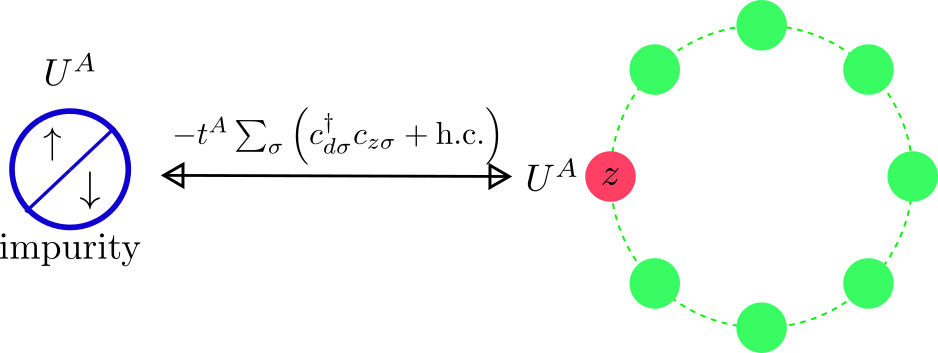
\includegraphics[width=0.6\textwidth]{../figures/gen_siam.png}
 	\caption{Correlated asymmetric Anderson molecule schematic version. It consists of an impurity site (blue) hybridising with a bath (ring) by hopping into and out of the zeroth site (pink). The other sites (green) form the rest of the bath. Just the impurity site and the zeroth site have onsite repulsion.}
 	\label{and_mol}
 \end{figure}
 This Hamiltonian is depicted in fig.~\ref{and_mol}. Such a Hamiltonian is, however, explicitly asymmetric between the sites 0 and 1 (the effective bath couples only to 1). To rectify that, we will symmetrize the coupling between the effective bath and the sites 0 and 1, by exchanging the sites 0 and 1. The resultant Hamiltonian is
 \begin{equation}\begin{aligned}
 	\underbrace{U^A\tau_{0 \uparrow}\tau_{0 \downarrow} + U^A\tau_{1 \uparrow}\tau_{1 \downarrow} - t^A\sum_{\sigma}\left(c^\dagger_{0\sigma}c_{1\sigma} + \text{h.c.}\right)}_\text{2-site Hubbard model} +\underbrace{- t^A\sum_{j \in \atop{\text{NN of 1}}}\left(c^\dagger_{1\sigma}c_{j\sigma} + \text{h.c.}\right)- t^A\sum_{j \in \atop{\text{NN of 0}}}\left(c^\dagger_{0\sigma}c_{j\sigma} + \text{h.c.}\right)}_\text{dimer \& eff. bath coupling} \\
 	- \underbrace{t^A \sum_{\left<ij \right>}^{\text{eff.} \atop{\text{bath}}}\left(c^\dagger_{i\sigma}c_{j\sigma} + \text{h.c.}\right)}_\text{eff. bath isolated}
 \end{aligned}\end{equation}

 To further simplify this Hamiltonian, \textit{we will combine the nearest neighbour sites of \(1\) and \(0\) into a single site}.
 \begin{equation}\begin{aligned}
 	c_z \equiv \left(\sum_{j \in \atop{\text{NN of 1}}} + \sum_{j \in \atop{\text{NN of 0}}}\right)c_{j}
 \end{aligned}\end{equation}
 This single site will act as the zeroth site of the effective bath, and it means that both sites of the Hubbard dimer hybridizes with the effective through just a single site. With this assumption, the Hamiltonian for "a Hubbard dimer hopping into an effective bath" takes the simple form
 \begin{equation}\begin{aligned}
 	\label{dimer_p_bat}
 	\tilde H^D = H^D(0,1) - t^D \sum_{\sigma}\left(c^\dagger_{0\sigma}c_{z\sigma} + c^\dagger_{1\sigma}c_{z\sigma} + \text{h.c.}\right) + \sum_{\vec k}^\text{eff. bath}\epsilon_{\vec k}\hat n_{\vec k}
 \end{aligned}\end{equation}
 \(H^D(0,1)\) is the Hubbard dimer Hamiltonian (shown in fig.~\ref{hubb-dim}):
 \begin{equation}\begin{aligned}
 	\label{dimer_ham}
 	H^D(0,1) \equiv -t^D\sum_\sigma\left( c^\dagger_{0\sigma}c_{1\sigma} + \text{h.c.} \right) + U^D\left( \tau_{0 \uparrow}\tau_{0 \downarrow} + \tau_{1 \uparrow}\tau_{1 \downarrow}\right)
 \end{aligned}\end{equation}
 \begin{figure}[!htb]
 	\centering
 	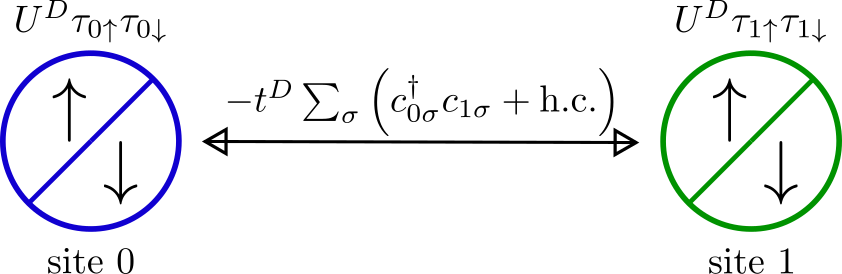
\includegraphics[width=0.4\textwidth]{../figures/hubb_dim.png}
 	\caption{Hubbard dimer schematic version. It again consists of two sites, like the Anderson molecule, but now both sites have onsite repulsion, and their is again inter-site hopping.}
 	\label{hubb-dim}
 \end{figure}
 This entire procedure is depicted in fig.~\ref{dimer-bath}.
 \begin{figure}[!htb]
 	\centering
 	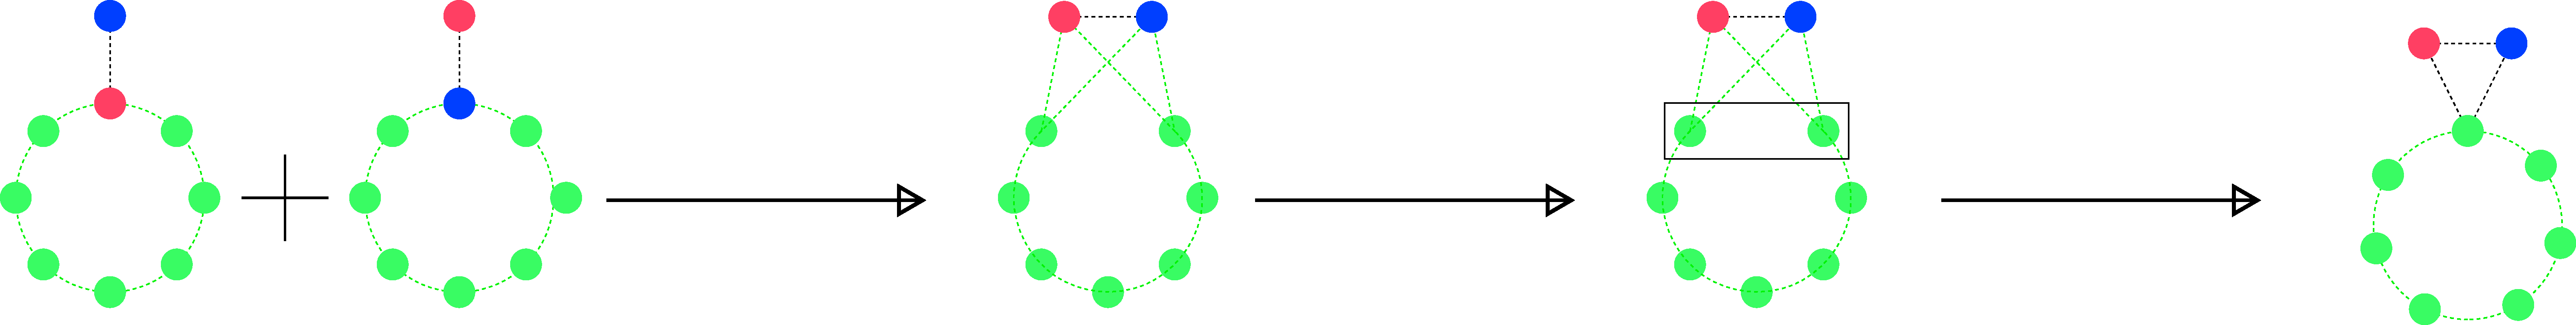
\includegraphics[width=\textwidth]{../figures/dimer_bath.pdf}
 	\caption{The process of symmetrizing the Rg fixed point Hamiltonian and then creating a dimer+bath Hamiltonian. We first add the asymmetric Hamiltonians to get a symmetrized Hamiltonian. In the symmetrized Hamiltonian, the dimer has \(w\) entry points into the bath, \(w\) being the coordination number of the lattice. We then merge these \(w\) lattice sites (enclosed in the black box) into a single lattice site.}
 	\label{dimer-bath} 
 \end{figure}
 We  can thus obtain a family of Hamiltonians \(\tilde H^D(i,j)\) obtained by setting \(0\) and \(1\) by setting the two sites of the dimer to any nearest-neighbour \(i,j\) on the lattice and the effective bath to the rest \(N-2\) sites of the lattice. The next step in the programme is to tile the real-space lattice with this dimer+bath Hamiltonian \(\tilde H_D\) to restore translational invariance (shown in a later section), and obtain a new Hubbard Hamiltonian, $\tilde H = T\left[ \tilde H^{D} \right] T^{-1}$, where $T$ denotes the operator that performs the set of iterative real-space translations, and enables the dimer Hamiltonian to span the target real-space lattice. We quote the final form of $\tilde H$ here to explain what the tiling means, but the explanation is given in a later section.
 \begin{equation}\begin{aligned}
 	\tilde H &= \frac{2}{Nw}\sum_{\left<ij\right>}\frac{1}{2(w-1)}\sum_{l \in \text{NN of (i,j)}}\tilde H^D((0,1,z) \to (i, j, l))\\
 		 &= \frac{2}{N}U^D\sum_{i} \tau_{i \uparrow}\tau_{i \downarrow} - \frac{2}{Nw}\left(1 + \frac{Nw}{2}\right)t^D\sum_{\left<ij\right>}\left(c^\dagger_{i\sigma}c_{j\sigma} + \text{h.c.}\right)
 \end{aligned}\end{equation}
 What that means is that we have placed the Hubbard dimer+bath system at all nearest neighbour pairs to reconstruct a new Hubbard model. If we assume that the tiling mostly rectifies the explicit symmetry-breaking made while choosing the auxiliary system as well as dropping the correlation on the bath sites, we can write
 \begin{equation}\begin{aligned}
 	\tilde H = \mathcal{U} H^H \mathcal{U}^{-1} = TZ\left[\mathcal{U}_A H^A \mathcal{U}_A^\dagger \right]Z^{-1} T^{-1}~,
 \end{aligned}\end{equation}
 where $\mathcal{U} = TZ\mathcal{U}_{A}$ is some transformation that is either a unitary, or, at the very least, a similarity transformation that maps from the original to the reconstructed Hubbard Hamiltonian. 
 The existence of $U$ is contingent on how good the approximations are.
 
 We mention the two approximations made along the entire journey from the original Hubbard model to the reconstructed one here.
 \begin{itemize}
 	\item We have replaced the full Hubbard model by an auxiliary system described by the SIAM Hamiltonian in eq.~\ref{clus_bath_siam}. The accuracy of this assumption is determined by the choice of the SIAM parameters, particular the self-energy and repulsion of the bath. As discussed before, the very choice of th cluster and bath spoil the translational invariance of the parent model.
 	\item We then perform a unitary RG on $H^A$. This leads to a fixed-point Hamiltonian $\mathcal{U}_A H^A \mathcal{U}_A^\dagger$. At this point, we go from the fixed point Hamiltonian to the dimer+bath Hamiltonian in eq.~\ref{dimer_p_bat}. If we represent this transformation from the fixed point Hamiltonian to the Hamiltonian in eq.~\ref{dimer_p_bat} by an operator \(Z\), we can write $H^D = Z\left[\mathcal{U}_A H^A \mathcal{U}_A^\dagger \right] Z^{-1}$. This constitutes the second approximation we make.
\end{itemize}
}


\section{Creating \(N-\)site Hubbard Hamiltonian from Hubbard dimer embedded in a bath}
Similar to the previous chapter, we will now tile the lattice with the two-site auxiliary model
\begin{equation}\begin{aligned}
	H_\text{aux} = \sum_{i=1,2} \left[- \frac{U}{2}\left(\hat n_{d_i \uparrow} - \hat n_{d_i \downarrow}\right)^2 + V\sum_{\sigma}\left(c^\dagger_{d_i\sigma}c_{0_i\sigma} + \text{h.c.}\right) + J \vec{S}_{d_i}\cdot\vec{s}_{0_i} - U_b\left(\hat n_{0_i \uparrow} - \hat n_{0_i \downarrow}\right)^2\right]\\
	 -t \sum_\sigma \left(c^\dagger_{d_1,\sigma}c_{d_2,\sigma} + \text{h.c.}\right) + \sum_{k\sigma}\epsilon_k \tau_{k\sigma}
\end{aligned}\end{equation}
For concreteness, we will consider a lattice of \(N\) lattice sites and \(w\) nearest neighbours for each site. Note that a uniform number of nearest neighbours means that there is perfect translational invariance on the lattice, which means there cannot be any edge sites. This is achieved by applying periodic boundary conditions on the edges of the lattice. For example, a square 2d lattice will have to be placed on a 2-torus.

The first step is to identity the two impurity sites \(d_1\) and \(d_2\) and the two bath sites \(0_1\) and \(0_2\) as sitting on a square arrangement of the lattice. \(d_i\) form one arm of the square, while \(0_i\) form the opposite arm.
This square arrangement is shown in fig.~\ref{square-arms}, and is dictated by the auxiliary model chosen and shown in fig.~\ref{two-imp-cluster}.
\begin{figure}[!htb]
	\centering
	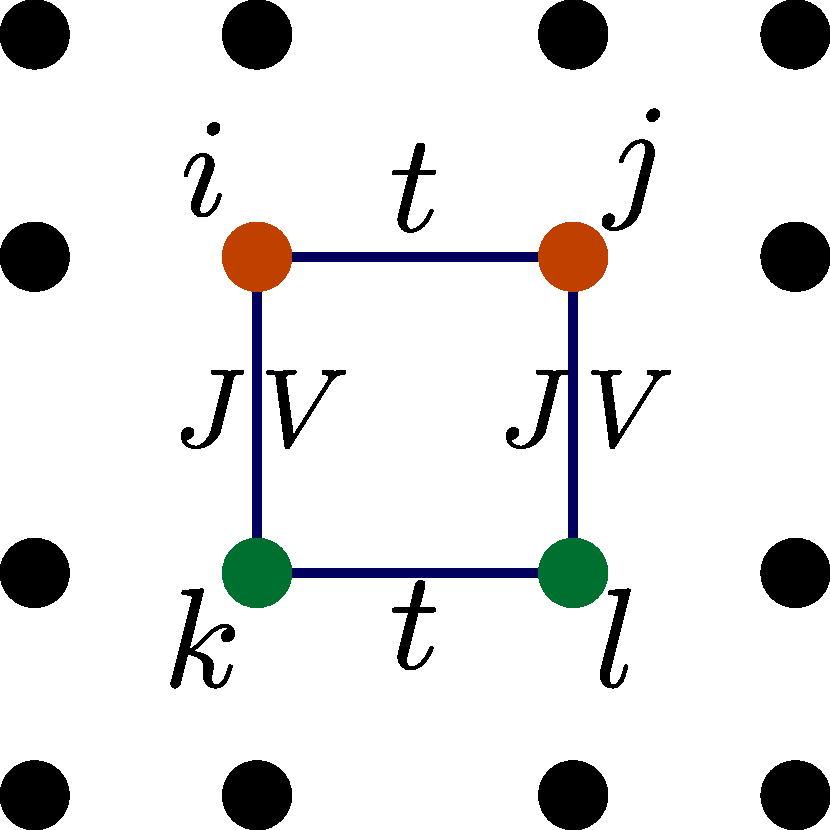
\includegraphics[width=0.3\textwidth]{../figures/square_arms.pdf}
	\caption{Placing the impurity and bath sites \(d_i,0_i\) on a chosen square of the lattice. The chosen square is marked in blue, the impurity sites in orange and the bath sites in green.}
	\label{square-arms}
\end{figure}
The sites at the vertices of the square are labelled as \(i,j,k,l\). With this identification, the Hamiltonian becomes
\begin{equation}\begin{aligned}
	H_\text{aux}(i,j,k,l) = \sum_{i=1,2} \left[- \frac{U}{2}\left(\hat n_{i \uparrow} - \hat n_{i \downarrow}\right)^2 - \frac{U}{2}\left(\hat n_{j \uparrow} - \hat n_{j \downarrow}\right)^2 + V\sum_{\sigma}\left(c^\dagger_{i\sigma}c_{k\sigma} + \text{h.c.} + c^\dagger_{j\sigma}c_{l\sigma} + \text{h.c.}\right) + J \vec{S}_{i}\cdot\vec{s}_{k} \right.\\
+ \left. J \vec{S}_{j}\cdot\vec{s}_{l} - U_b\left(\hat n_{k \uparrow} - \hat n_{k \downarrow}\right)^2 - U_b\left(\hat n_{l \uparrow} - \hat n_{l \downarrow}\right)^2\right] -t \sum_\sigma \left(c^\dagger_{i,\sigma}c_{j,\sigma} + \text{h.c.}\right) -t \sum_{\left<m,n \right>, \sigma}^{m,n \notin \left\{i,j\right\}}\left(c^\dagger_{m\sigma,n\sigma} + \text{h.c.}\right) 
\end{aligned}\end{equation}
As before, the kinetic energy part sums over all nearest neighbour pairs that involve neither \(i\) nor \(j\). For a given arm \(i-j\), the square can be rotated along the axis \(i-j\) to give one square arrangements for each dimension perpendicular to the axis along \(i-j\). Since there are \(w/2\) dimensions, the number of such squares is \(w/2 - 1\). For each such square, we can obtain another square by reflecting the square in the plane of \(i-j-l-k-i\) and across the line \(i-j\). The total number of squares is therefore \(w - 2\). The upshot is that given \(i-j\), there are multiple ways of choosing \(k\); if \(\left\{\vec a\right\}\) represents the set of \(w\) primitive vectors that connect a particular lattice site to its nearest neighbours, \(k\) can be situated at all \(\vec r_i + \vec a\) for which \(\vec a \times \left(\vec r_j - \vec r_i\right) \neq 0\). Choosing \(k\) then automatically fixes \(l\) at \(\vec r_j + \vec a\). The condition \(\vec a \times \left(\vec r_j - \vec r_i\right) \neq 0\) simply means we only take those \(\vec a\) that are perpendicular to \(\vec r_j - \vec r_i\). Since there are \(w\) number of \(\vec a\) in total and 2 of them are parallel, the total number of choices of \(k,l\) is \(w-2\).  For a 2D lattice, we have \(w=4\), so there are only two possible choices of the square. They are shown in fig.~\ref{square-arms-all}.
\begin{figure}[!htb]
	\centering
	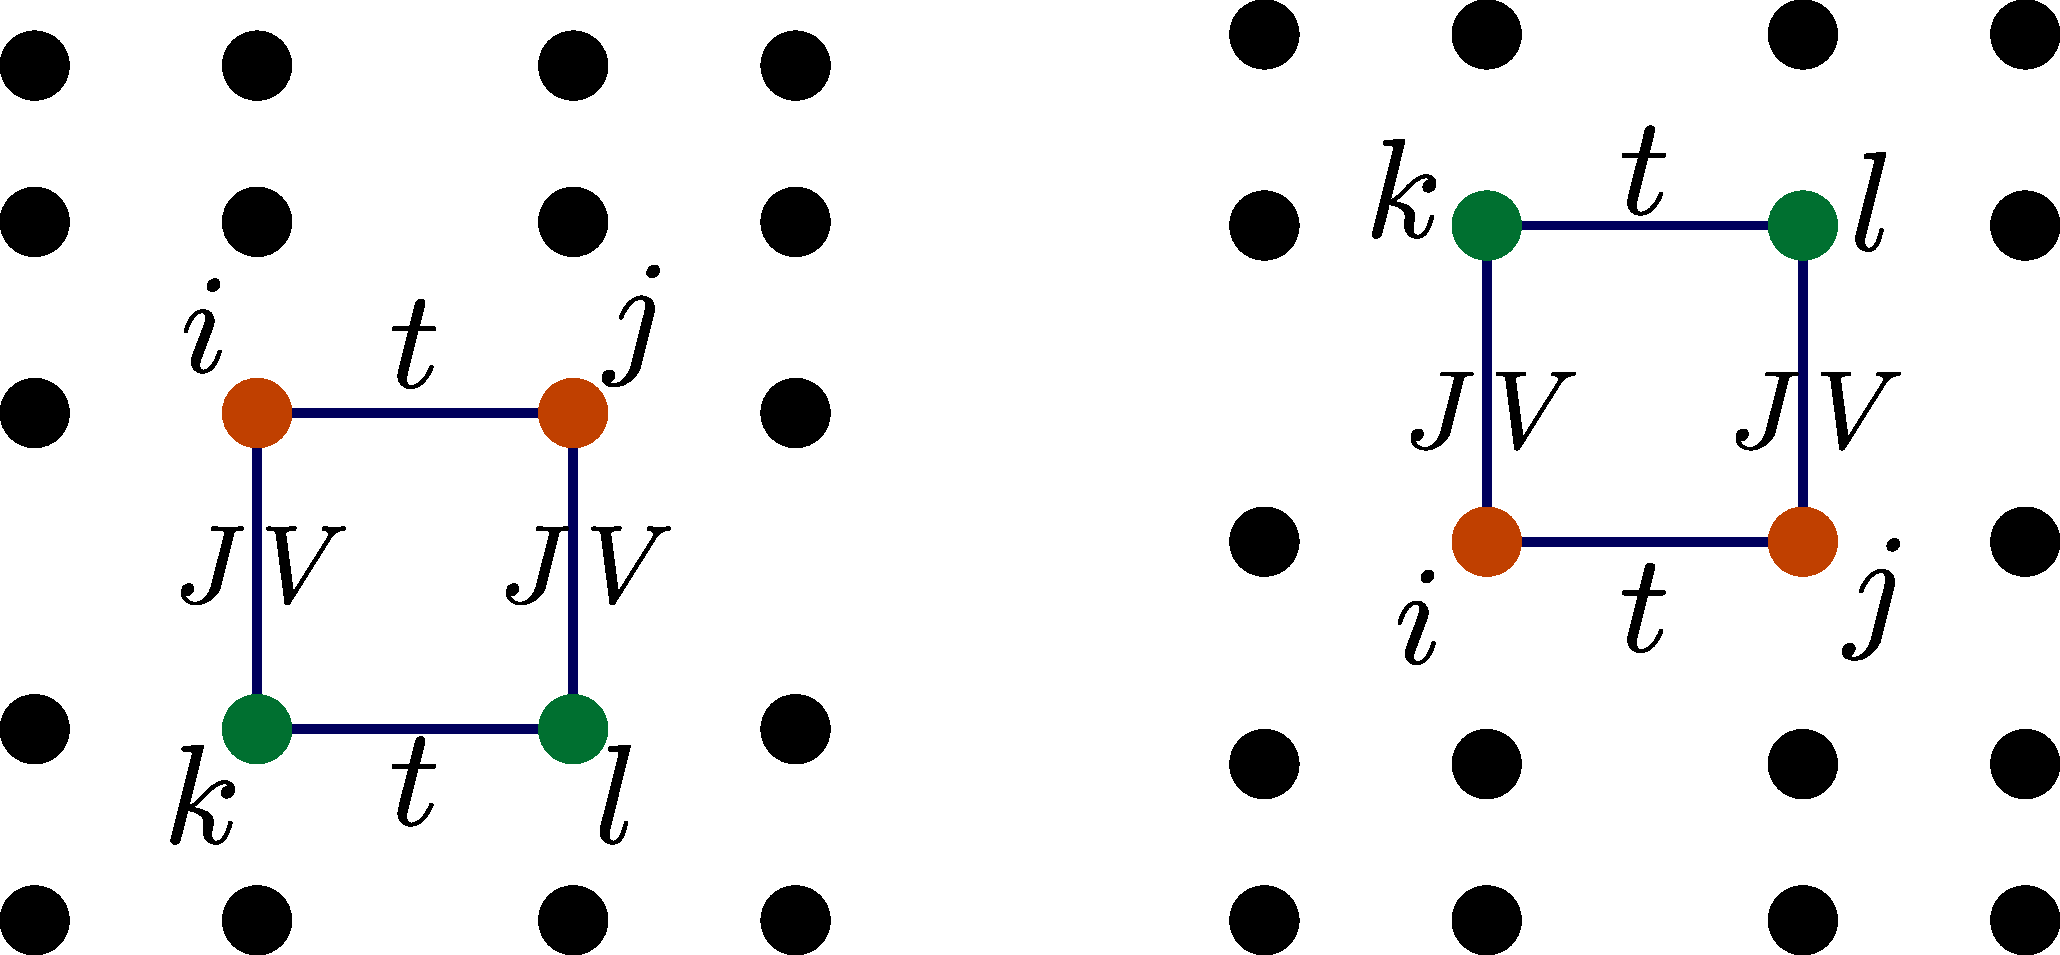
\includegraphics[width=0.6\textwidth]{../figures/square_arms_all.pdf}
	\caption{Placing the impurity and bath sites \(d_i,0_i\) on a chosen square of the lattice. The chosen square is marked in blue, the impurity sites in orange and the bath sites in green.}
	\label{square-arms-all}
\end{figure}

The Hamiltonian for an arm \(i-j\) is then obtained by averaging over these squares:
\begin{equation}\begin{aligned}
	H_\text{aux}(i,j) = \frac{1}{w - 2}\sum_{\vec r_k = \vec r_i + \vec a \atop{\vec r_l = \vec r_j + \vec a}}^{\vec a \times \left(\vec r_j - \vec r_i\right) \neq 0}H_\text{aux}(i,j,k,l)
\end{aligned}\end{equation}
The final step is to sum over all nearest neighbour arms \(i-j\):
\begin{equation}\begin{aligned}
	\label{22siam_to_hubb}
	H_\text{full} = \sum_{\left<i,j\right>}\frac{1}{w - 2}\sum_{\vec r_k = \vec r_i + \vec a \atop{\vec r_l = \vec r_j + \vec a}}^{\vec a \times \left(\vec r_j - \vec r_i\right) \neq 0}H_\text{aux}(i,j,k,l)
\end{aligned}\end{equation}

There are four kinds of terms:
\begin{itemize}
	\item the first kind, \(A(i), A(j)\), depend only on either \(i\) or \(j\). They can be summed over easily by noting that the internal summation gives a constant factor of \(w-2\) which is canceled by the factor of \(1/(w-2)\) in the front, and the external summation gives \(\sum_{i,j}A(i) = \frac{w}{2} \sum_i A(i)\), because \(i\) is a member of \(w/2\) distinct nearest-neighbour pairs. 
	\item The second kind, \(B(i,j)\) depends on both \(i\) and \(j\). The internal summation is again cancelled by the prefactor. The external summation simply sums over all nearest-neighbour values of \(A(i,j)\).
	\item The third kind, \(C(i,k), C(j,l)\), depend on \(i\) and \(k\). Here, the total summation \(\sum_{i,j,k}C(i,k)\) gives \((w-2)\sum_{\left<i,k\right>}\left(C(i,k) + C(k,i)\right)\), because the pair \((i,k)\) occurs \(w-2\) times corresponding to the \(w-2\) vectors \(\vec r_j - \vec r_i\) that are perpendicular to \(\vec r_i - \vec r_k\). The factor is again cancelled by the existing prefactor. 
	\item The fourth kind, \(D(k), D(l), E(k,l)\), depend on just \(k\), just \(l\) or both \(k\) and \(l\). For each pair \(i-j\) in the external summation, the particular pair \(k-l\) appears only once. When \(i-j\) is summed over, a factor of \(2(w/2-1)\) is generated because there are that many squares that involve \(k-l\). This factor cancels the inverse factor in front, giving \(\sum_{\left<k\right>} D(k), \sum_{\left<k,l \right>}E(k,l)\).
\end{itemize}

 The full Hamiltonian reads
\begin{equation}\begin{aligned}
	H_\text{full} =& w\sum_i\left[- \frac{U}{2}\left(\hat n_{i \uparrow} - \hat n_{i \downarrow}\right)^2\right] - t\sum_{\left<i,j \right>,\sigma}\left(c^\dagger_{i\sigma}c_{j\sigma} + \text{h.c.}\right) + 4V\sum_{\sigma, \left<i,k\right>}\left(c^\dagger_{i\sigma}c_{k\sigma} + \text{h.c.}\right)\\
		      &+ 4J \sum_{\left<i,k\right>}\left(\vec{S}_{i}\cdot\vec{S}_{k}\right) - 2 U_b\sum_k\left(\hat n_{k \uparrow} - \hat n_{k \downarrow}\right)^2 - \frac{Nw/2}{w-2}t\sum_{\left<i,j \right>,\sigma}\left(c^\dagger_{i\sigma}c_{j\sigma} + \text{h.c.}\right)\\
	=& -\frac{1}{2}\left(Uw + 4U_b\right)\sum_i \left(\hat n_{i \uparrow} - \hat n_{i \downarrow}\right)^2 - \left(\frac{Nw/2}{w-2}t + t - 4V\right) \sum_{\left<i,j \right>,\sigma}\left(c^\dagger_{i\sigma}c_{j\sigma}\right) + 4J \sum_{\left<i,j \right>} \vec{S}_i\cdot\vec{S}_j
\end{aligned}\end{equation}
The bulk model hence obtained is again a Hubbard-Heisenberg model. In eq.~\ref{2siam_to_hubb}, the total number of terms in the outer summation is \(Nw/2\). In order to make sure that this full Hamiltonian scales as \(N\), we divide this by \(w/2\):
\begin{equation}\begin{aligned}
	\label{2siam_to_hubb}
	H_\text{full} &= \frac{2}{w}\sum_{\left<i,j\right>} H_\text{aux}(i,j) = \frac{2}{w}\sum_{\left<i,j\right>}\frac{1}{w - 2}\sum_{\vec r_k = \vec r_i + \vec a \atop{\vec r_l = \vec r_j + \vec a}}^{\vec a \times \left(\vec r_j - \vec r_i\right) \neq 0}H_\text{aux}(i,j,k,l)\\
		      &= -\frac{1}{2}\left(2U + 8U_b/w\right)\sum_i \left(\hat n_{i \uparrow} - \hat n_{i \downarrow}\right)^2 - \left(\frac{N}{w-2}t + 2t/w - 8V/w\right) \sum_{\left<i,j \right>,\sigma}\left(c^\dagger_{i\sigma}c_{j\sigma}\right) + 8J/w \sum_{\left<i,j \right>} \vec{S}_i\cdot\vec{S}_j
\end{aligned}\end{equation}
The mappings between the parameters of the auxiliary model and the bulk are
\begin{equation}\begin{aligned}
	t_\text{H-H} = \left(\frac{N}{w-2}t + 2t/w - 8V/w\right),~ ~ ~ U_\text{H-H} = 2U + 8U_b/w,~ ~ ~ J_\text{H-H} = 8J/w
\end{aligned}\end{equation}

We could have also inserted a spin-exchange interaction between the two impurities in the auxiliary model:
\begin{equation}\begin{aligned}
	H_\text{aux} = \sum_{i=1,2} \left[- \frac{U}{2}\left(\hat n_{d_i \uparrow} - \hat n_{d_i \downarrow}\right)^2 + V\sum_{\sigma}\left(c^\dagger_{d_i\sigma}c_{0_i\sigma} + \text{h.c.}\right) + J \vec{S}_{d_i}\cdot\vec{s}_{0_i} - U_b\left(\hat n_{0_i \uparrow} - \hat n_{0_i \downarrow}\right)^2\right] -t \sum_\sigma \left(c^\dagger_{d_1,\sigma}c_{d_2,\sigma} + \text{h.c.}\right)\\
	+ J_d \vec{S}_{d_1}\cdot\vec{S}_{d_2} + \sum_{k\sigma}\epsilon_k \tau_{k\sigma}
\end{aligned}\end{equation}
In the presence of this term, the bulk Hamiltonian remains the same, but the expression of \(J_\text{H-H}\) changes. Since this term is similar in form to the term preceding it, we can easily obtain the updated expression:
\begin{equation}\begin{aligned}
	J_\text{H-H} = \frac{2}{w}\left(4J + 2J_d\right)
\end{aligned}\end{equation}


\section{Single-particle Green's function}
We now define the Greens function {\it operators}:
\begin{equation}\begin{aligned}
	\mathcal{G}_{H-H} = \frac{1}{\omega^\prime - \left(H_{H-H} - E_\text{gs}^\prime\right) }, \mathcal{G}_\text{aux}(i,j) = \frac{1}{\omega - \left(\mathcal{H}_\text{aux}(i,j) - E_\text{gs}\right)}
\end{aligned}\end{equation}
Here, \(E_\text{gs}\) and \(\omega\) are the ground state energy and frequency scale for the auxiliary model Hamiltonian, while the primed quantities \(E_\text{gs}^\prime\) and \(\omega^\prime\) are the same quantities but for the full model \(\mathcal{H}_{H-H}\). While the auxiliary model is intensive, the full Hamiltonian is extensive and scales as \(N\):
\begin{equation}\begin{aligned}
	H_\text{full} &= \frac{2}{w}\sum_{\left<i,j\right>} H_\text{aux}(i,j) \sim N H_\text{aux}(d_1,d_2)~.
\end{aligned}\end{equation}
This means that we must have \(\omega^\prime = N\omega\) and \(E_\text{gs}^\prime = N E_\text{gs}\).
Rewriting eq.~\ref{2siam_to_hubb} in terms of the operators \(\mathcal{G}\), we get
\begin{equation}\begin{aligned}
\sum_{\left<i,j \right>} \left(\omega + E_\text{gs} - \mathcal{G}^{-1}_\text{aux}(i,j)\right) = N\omega + N E_\text{gs} - \mathcal{G}^{-1}_{H-H} \implies \sum_{\left<i,j \right>} \mathcal{G}^{-1}_\text{aux}(i,j) = \mathcal{G}^{-1}_{H-H}~,
\end{aligned}\end{equation}
We will now take matrix elements of the full Greens function and obtain these matrix elements in terms of those of the auxiliary model. Let \(\left\{ \ket{\Phi}_n \right\} \) be the set of eigenstates of \(\mathcal{H}_\text{aux}\), and \(\ket{\Phi}_0\) be the groundstate. We assume that the ground state of \(H_{H-H}\) is captured well by the auxiliary model, such that the real-space diagonal matrix element for particle propagation is obtained by sandwiching the Greens function between the states \(c^\dagger_{i\sigma}\ket{\Phi}_0\):
\begin{equation}\begin{aligned}
	\left(\mathcal{G}^{-1}_{H-H}\right)^p_{ii} \equiv \braket{\Phi_0 | c_{i\sigma} \mathcal{G}^{-1}_{H-H} c^\dagger_{i\sigma} | \Phi_0} = \sum_{\left<k,l\right>} \braket{\Phi_0 | c_{i\sigma} \mathcal{G}^{-1}_\text{aux}(k,l) c^\dagger_{i\sigma} | \Phi_0}
\end{aligned}\end{equation}
The superscript \(p\) indicates that this is the particle propagation matrix element. Under the auxiliary model approximation, we ignore the virtual entanglement between separate clusters. Therefore, the only operators \(\mathcal{G}^{-1}_\text{aux}(k,l)\) that affect the matrix element are those that satisfy \(i \in \left(k,l\right)\). There are \(w\) such pairs: \(\left\{k,l\right\} = \left\{i,j\right\} \forall~ j \in \text{NN of i}\). Moreover, because of translation invariance, all \(j \in \text{NN of i}\) are equivalent. These configurations are shown in fig.~\ref{diag_conrib}.
\begin{figure}[!htb]
	\centering
	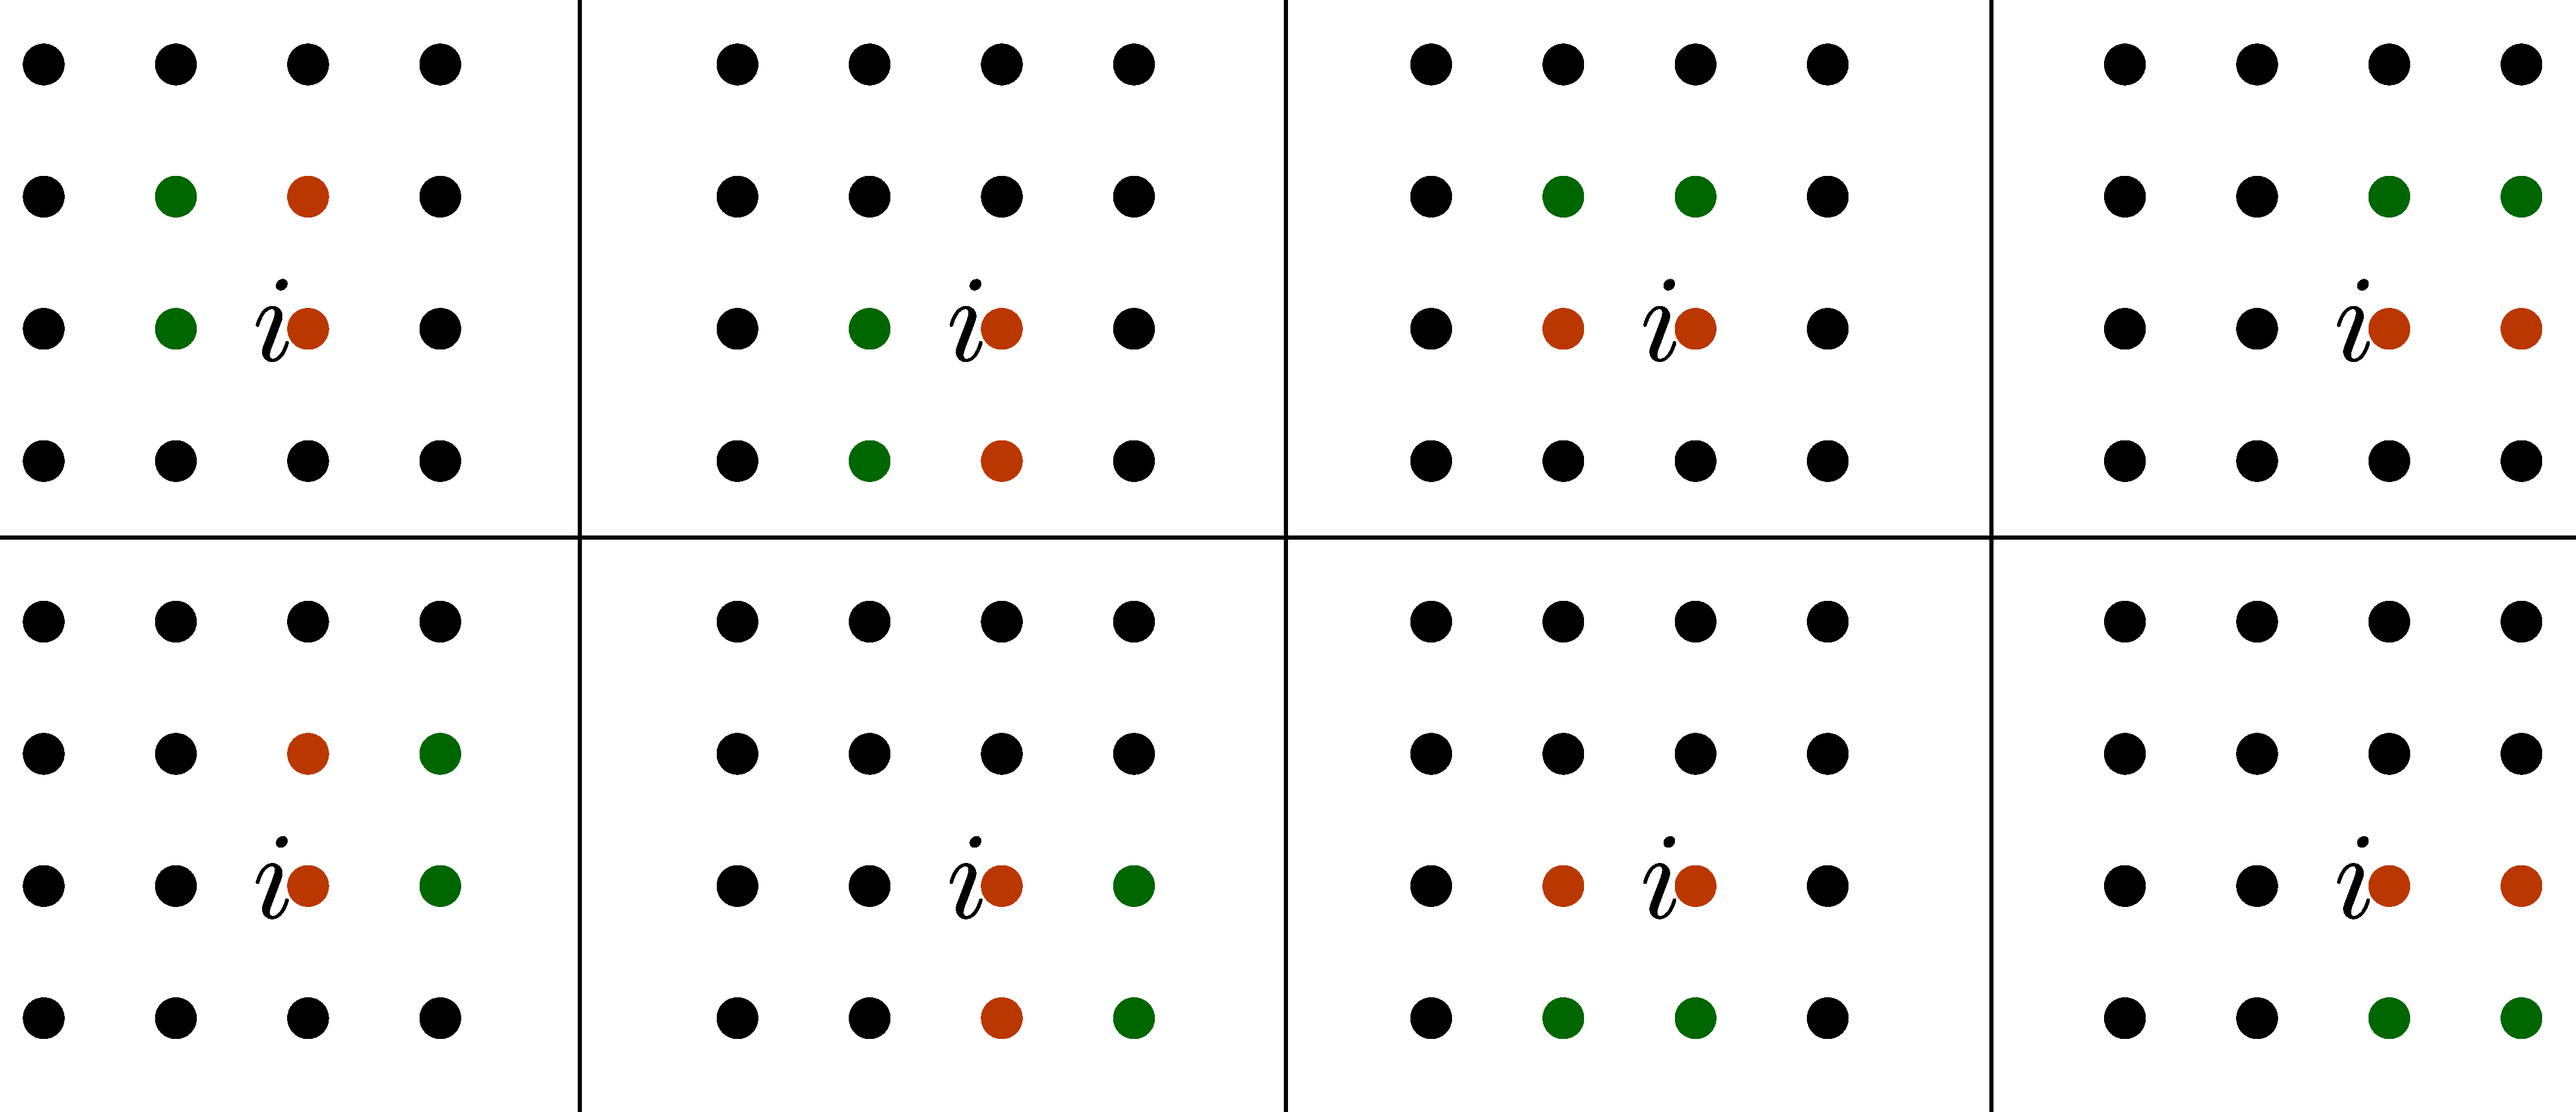
\includegraphics[width=0.8\textwidth]{../figures/diagonal_contributors.pdf}
	\caption{The various configurations of auxiliary models that contribute to the diagonal matrix element at site \(i\). Orange colour represents impurities and green represents bath sites.}
	\label{diag_conrib}
\end{figure}

\begin{equation}\begin{aligned}
	\left(\mathcal{G}^{-1}_{H-H}\right)^p_{ii} = \sum_{\left<k,l\right>} \braket{\Phi_0 | c_{i\sigma} \mathcal{G}^{-1}_\text{aux}(k,l) c^\dagger_{i\sigma} | \Phi_0} = \frac{2}{w} \times w \times \braket{\Phi_0 | c_{i\sigma} \mathcal{G}^{-1}_\text{aux}(i, i+1) c^\dagger_{i\sigma} | \Phi_0} = 2\braket{\Phi_0 | c_{d_1\sigma} \mathcal{G}^{-1}_\text{aux}(d_1,d_2) c^\dagger_{d_1\sigma} | \Phi_0}
\end{aligned}\end{equation}
where we have identified site \(i\) in the auxiliary model as one of the impurities \(d_1\). We could very well have chosen \(d_2\) since the model is symmetric in \(d_1,d_2\). \(\mathcal{G}^{-1}_\text{aux}(d_1,d_2)\) is the Greens operator corresponding to the Hamiltonian in eq.~\ref{dimer_ham}.

By inserting \(1 = \sum_n \ket{\Phi_n}\bra{\Phi_n}\) on both sides of \(\mathcal{G}^{-1}_\text{aux}\), we get from the spectral representation
\begin{equation}\begin{aligned}
	\left(\mathcal{G}^{-1}_{H-H}(\omega)\right)^p_{ii} = 2\sum_{m,n} \braket{\Phi_0 | c_{d_1\sigma} \ket{\Phi_m}\bra{\Phi_m}\mathcal{G}^{-1}_\text{aux} \ket{\Phi_n}\bra{\Phi_n} c^\dagger_{d_1\sigma} | \Phi_0} = 2\sum_{n} |d^p_{1,n}|^2 \left(\mathcal{G}^{-1}\left(\omega\right) _\text{aux}\right)_{nn}
\end{aligned}\end{equation}
There we used the fact that since \(\ket{\Phi_m}\) are eigenstates of \(\mathcal{H}_\text{aux}\) and hence of \(\mathcal{G}^{-1}_\text{aux}\), we can set \(m=n\). We also defined \(d^p_{i,n} = \bra{\Phi_n}c^\dagger_{d_i\sigma}\ket{\Phi_0}\). The hole propagation matrix element can be obtained similarly:
\begin{equation}\begin{aligned}
	\left(\mathcal{G}^{-1}_{H-H}(-\omega)\right)^h_{ii} = 2\sum_{n} |d^h_{1,n}|^2 \left(\mathcal{G}^{-1}_\text{aux}(-\omega)\right)_{nn} 
\end{aligned}\end{equation}
where \(d^h_{i,n} = \bra{\Phi_n}c_{d_i\sigma}\ket{\Phi_0}\).

The off-diagonal matrix elements between two nearest-neighbour sites \(i\) and \(i+1\) can also be obtained similarly. Several  auxiliary models can contribute to such a matrix element:
\begin{itemize}
	\item those auxiliary models that have \(i\) and \(i+1\) as the two impurities. These give the contribution \\
		\(\braket{\Phi_0 | c_{d_1\sigma} \mathcal{G}^{-1}_\text{aux}(d_1,d_2) c^\dagger_{d_2\sigma} | \Phi_0}\). 
	\begin{equation}\begin{aligned}
		\frac{2}{w}\braket{\Phi_0 | c_{d_1\sigma} \mathcal{G}^{-1}_\text{aux}(d_1,d_2) c^\dagger_{d_2\sigma} | \Phi_0} = \frac{2}{w}\sum_{n} \left(d^p_{1,n}\right)^*d^p_{2,n} \left(\mathcal{G}^{-1}\left(\omega\right) _\text{aux}\right)_{nn}
	\end{aligned}\end{equation}
	\item those that have \(i\) as an impurity and \(i+1\) as the corresponding bath site. There will be \(w-2\) of these in number:
	\begin{equation}
		(w-2) \times \frac{2}{w}\frac{1}{w-2}\braket{\Phi_0 | c_{d_1\sigma} \mathcal{G}^{-1}_\text{aux}(d_1,d_2) c^\dagger_{0_1\sigma} | \Phi_0} = \frac{2}{w}\left(d^p_{1,n}\right)^* z^p_{1,n} \left(\mathcal{G}^{-1}\left(\omega\right) _\text{aux}\right)_{nn}
	\end{equation}
		where \(z^p_{i,n} = \braket{\Phi_n | c^\dagger_{0_i,\sigma} | \Phi_0}\).
	\item those that have \(i+1\) as an impurity site and \(i\) as the corresponding bath site. There are again \(w-2\) of these:
	\begin{equation}
		(w-2) \times \frac{2}{w}\frac{1}{w-2}\braket{\Phi_0 | c_{0_1\sigma} \mathcal{G}^{-1}_\text{aux}(d_1,d_2) c^\dagger_{d_1\sigma} | \Phi_0} = \frac{2}{w}\left(z^p_{1,n}\right)^* d^p_{1,n} \left(\mathcal{G}^{-1}\left(\omega\right) _\text{aux}\right)_{nn}
	\end{equation}
\end{itemize}
These choices are shown in fig.~\ref{off-diag-contrib}.
\begin{figure}[!htb]
	\centering
	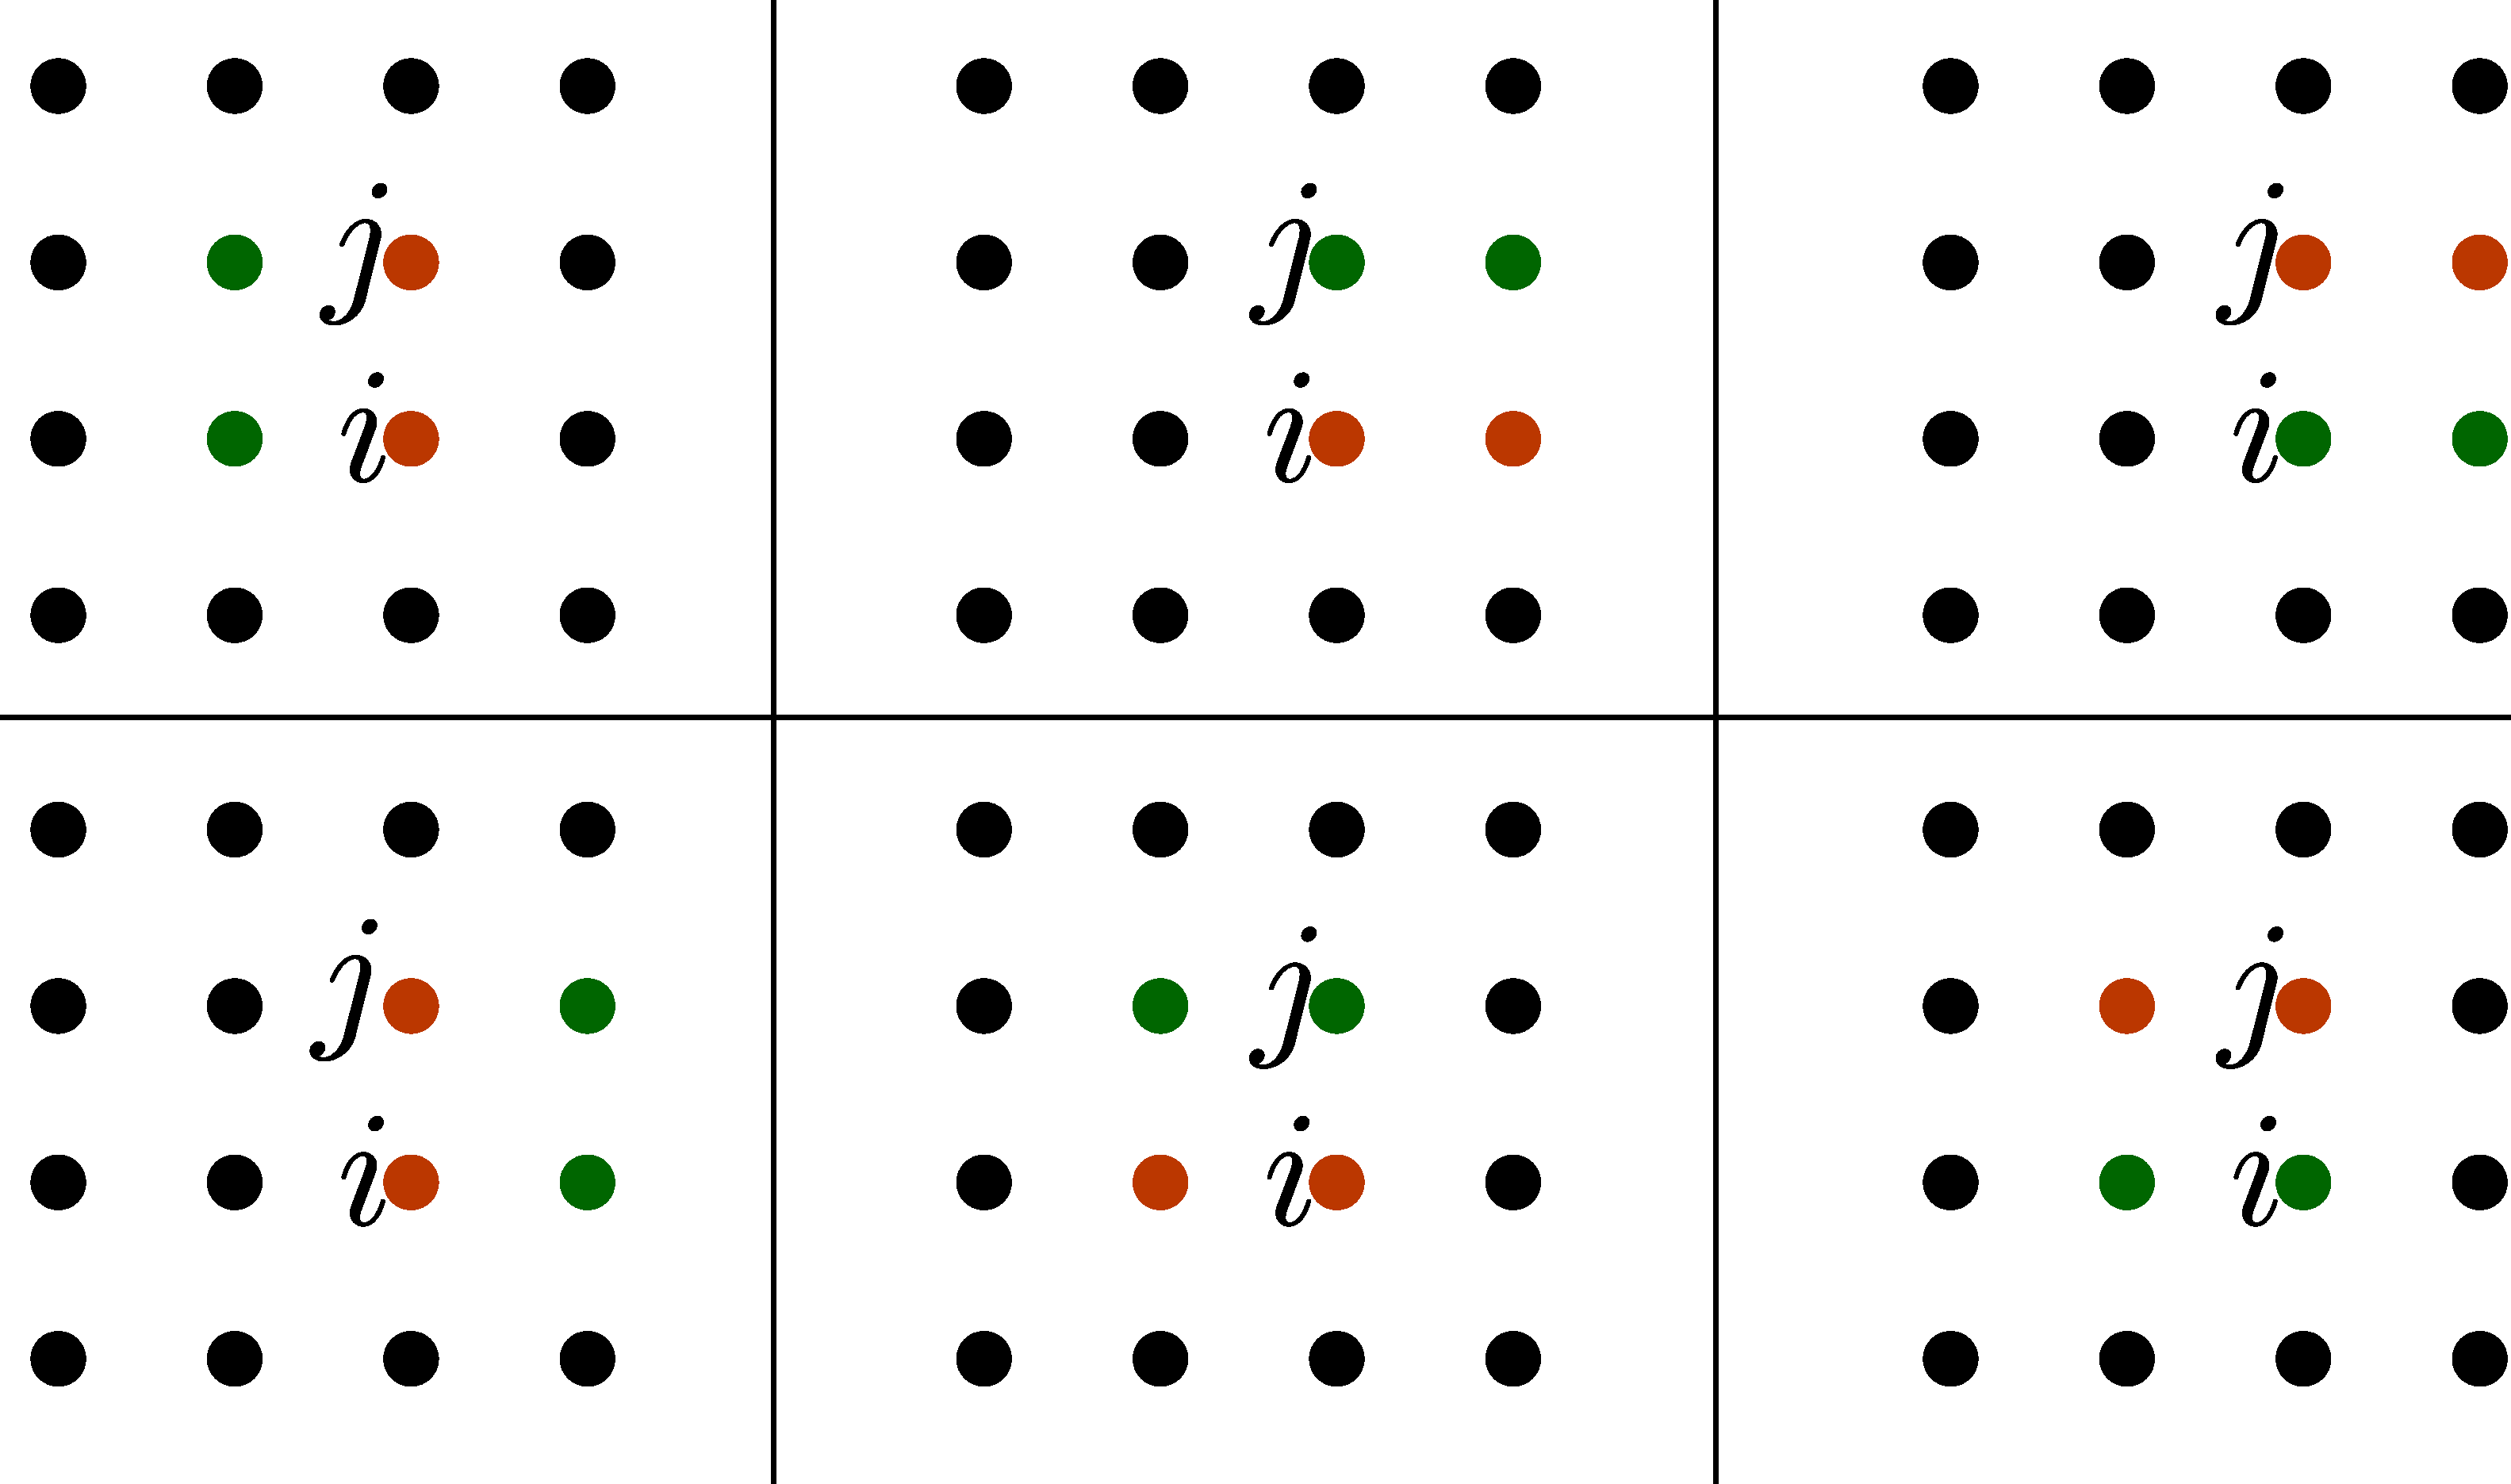
\includegraphics[width=0.5\textwidth]{../figures/offdiagonal_contributors.pdf}
	\caption{Auxiliary models that contribute to the off-diagonal matrix element. \(j \equiv i+1\)}
	\label{off-diag-contrib}
\end{figure}

Adding all contributions gives
\begin{equation}\begin{aligned}
	\left(\mathcal{G}^{-1}_{H-H}\left(\omega\right) \right)^p_{i,i+1} = \frac{2}{w} \sum_n \left[\left(d^p_{1,n}\right)^*d^p_{2,n} + \left(d^p_{1,n}\right)^* z^p_{1,n} + \text{h.c.}\right] \left(\mathcal{G}^{-1}_\text{aux}(\omega) \right)_{nn}
\end{aligned}\end{equation}
The hole counterpart is
\begin{equation}\begin{aligned}
	\left(\mathcal{G}^{-1}_{H-H}\left(-\omega\right) \right)^h_{i,i+1} = \frac{2}{w} \sum_n \left[\left(d^h_{1,n}\right)^*d^h_{2,n} + \left(d^h_{1,n}\right)^* z^h_{1,n} + \text{h.c.}\right] \left(\mathcal{G}^{-1}_\text{aux}(-\omega) \right)_{nn}
\end{aligned}\end{equation}
where \(z^h_{i,n} = \bra{\Phi_n}c_{z_i\sigma}\ket{\Phi_0}\).

The off-diagonal matrix element between next-to-nearest-neighbour sites \(i,i+2\) can also be obtained, provided their positions are related as \(\vec r_{i+2} = \vec r_i + \vec a + \vec a^\prime\), where \(\vec a\) and \(\vec a^\prime\) are primitive vectors that connect any lattice site to its nearest-neighbours, and \(\vec{a}\cdot\vec{a}^\prime = 0\). This is shown in fig.~\ref{next-near}. 

\par\noindent
\begin{minipage}{0.6\textwidth}
The essence is that the two sites have to form the two most separated vertices of a right-angled triangle. To find the auxiliary models that contribute to this matrix element, note that there is only one square that can be formed keeping both \(i\) and \(i+2\) on it - we call this square \(ABCD\), where \(A\) is the vertex \(i\) and \(C\) is the vertex \(i+2\). We can set \(A=d_1, C=0_2\). The other two vertices \(B\) and \(D\) can have two possible configurations:\(B=d_2,D=0_1\) and \(B=0_1,D=d_2\). Two more configurations can be obtained by taking each of these two configurations and keeping \(B,D\) unchanged but exchanging \(A\) and \(C\). These four configurations are shown in fig.~\ref{nn-configs}. 
\end{minipage}
\hspace*{\fill}
\begin{minipage}{0.35\textwidth}
	\centering
	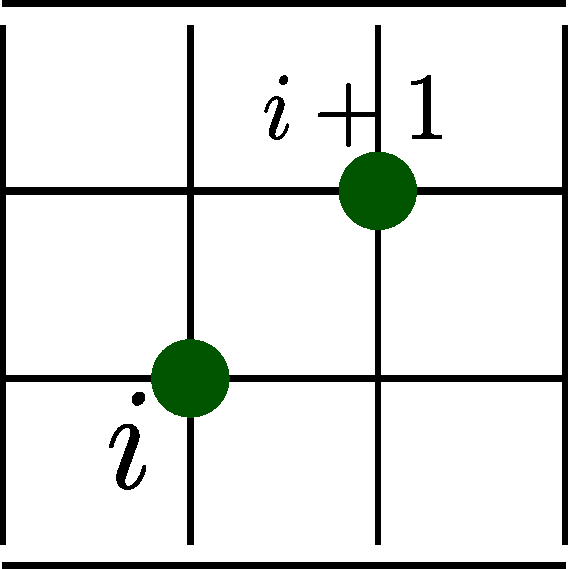
\includegraphics[width=0.9\textwidth]{../figures/next-near.pdf}
	\captionof{figure}{The kind of next-nearest neighbour sites that can be connected by the auxiliary model.}
	\label{next-near}
\end{minipage}

\begin{figure}[!htb]
	\centering
	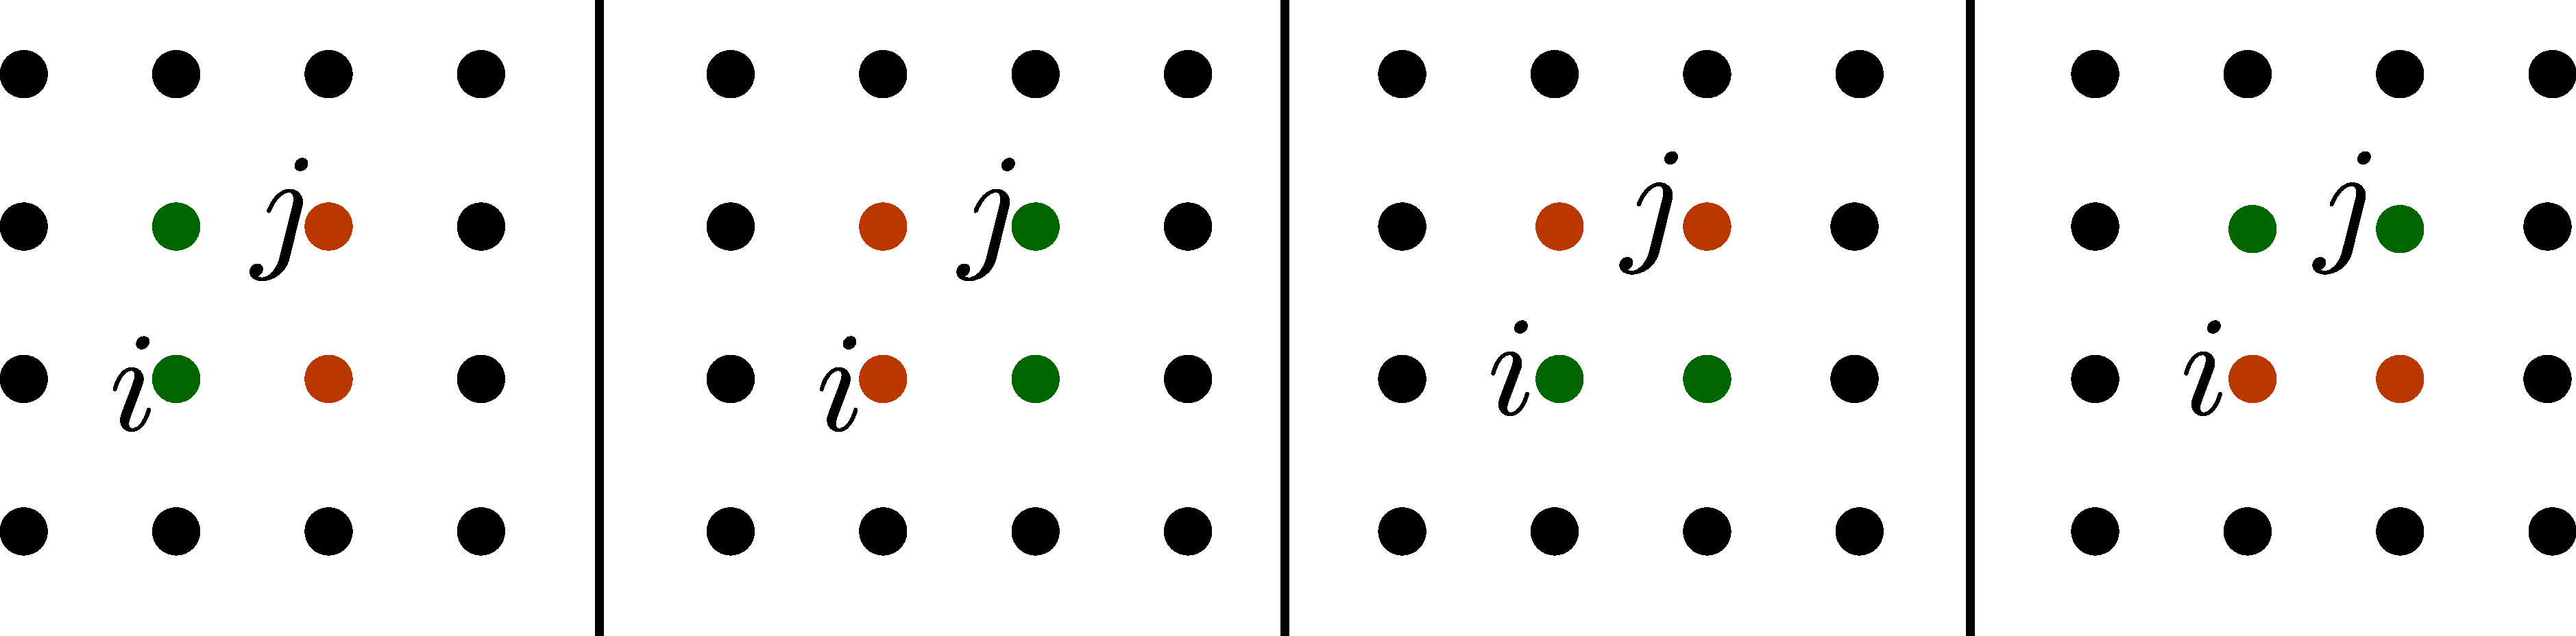
\includegraphics[width=0.8\textwidth]{../figures/nn-offdiagonal_contributors.pdf}
	\caption{Auxiliary model configurations that contribute to the next-nearest neighbour matrix elements. \(j \equiv i+2\)}
	\label{nn-configs}
\end{figure}

These four configurations give
\begin{equation}\begin{aligned}
	\left(\mathcal{G}_\text{H-H}^{-1}\left( \omega \right) \right)^p_{i,i+2} &= \frac{2}{w(w-2)}\left[\braket{\Phi_0|c_{d_1\sigma}\mathcal{G}^{-1}_\text{aux}(d_1,d_2)c^\dagger_{0_2,\sigma}|\Phi_0} + \braket{\Phi_0|c_{0_2\sigma}\mathcal{G}^{-1}_\text{aux}(d_1,d_2)c^\dagger_{d_1,\sigma}|\Phi_0}\right] \\
										 &= \frac{2}{w(w-2)}\sum_n \left[\left(d^p_{1,n}\right)^* z^p_{2,n} + \left(z^p_{2,n}\right)^* d^p_{1,n}\right] \left(\mathcal{G}^{-1}_\text{aux}(\omega)\right)_{nn}
\end{aligned}\end{equation}


In summary, the spectral representation of the matrix elements of the inverse Greens operators are given by
\begin{gather}
\label{green_eq_final_2siam}
	\left(\mathcal{G}^{-1}_{H-H}(\omega)\right)^p_{ii} = \sum_{n} |d^p_{1,n}|^2 \left(\mathcal{G}^{-1}_\text{aux}(\omega)\right)_{nn}~,\\
	\left(\mathcal{G}^{-1}_{H-H}(-\omega)\right)^h_{ii} = \sum_{n} |d^h_{1,n}|^2 \left(\mathcal{G}^{-1}_\text{aux}(-\omega)\right)_{nn}~,\\
	\left(\mathcal{G}^{-1}_{H-H}\left(\omega\right) \right)^p_{i,i+1} = \frac{2}{w} \sum_n \left[\left(d^p_{1,n}\right)^*d^p_{2,n} + \left(d^p_{1,n}\right)^* z^p_{1,n} + \text{h.c.}\right] \left(\mathcal{G}^{-1}_\text{aux}(\omega) \right)_{nn}~,\\
	\left(\mathcal{G}^{-1}_{H-H}\left(-\omega\right) \right)^h_{i,i+1} = \frac{2}{w} \sum_n \left[\left(d^h_{1,n}\right)^*d^h_{2,n} + \left(d^h_{1,n}\right)^* z^h_{1,n} + \text{h.c.}\right] \left(\mathcal{G}^{-1}_\text{aux}(-\omega) \right)_{nn}~,\\
	\left(\mathcal{G}_\text{H-H}^{-1}\left( \omega \right) \right)^p_{i,i+2} = \frac{2}{w(w-2)}\sum_n \left[\left(d^p_{1,n}\right)^* z^p_{2,n} + \left(z^p_{2,n}\right)^* d^p_{1,n}\right] \left(\mathcal{G}^{-1}_\text{aux}(\omega)\right)_{nn}~,\\
	\left(\mathcal{G}_\text{H-H}^{-1}\left( -\omega \right) \right)^h_{i,i+2} = \frac{2}{w(w-2)}\sum_n \left[\left(d^h_{1,n}\right)^* z^h_{2,n} + \left(z^h_{2,n}\right)^* d^h_{1,n}\right] \left(\mathcal{G}^{-1}_\text{aux}(\omega)\right)_{nn}~.
\end{gather}

In order to obtain the matrix elements of the Greens operators \(\mathcal{G}_{H-H}\) (as compared to its inverse), we note that we have just observed that the matrix elements of the inverse Greens operators are related to the matrix elements of another inverse operator through some coefficients. We can, therefore, use the identity
\begin{equation}\begin{aligned}
\left(\hat O\right)_{ij} = \bra{i} \hat O \ket{j} = \sum_{m,n} \braket{i|m} \left(\hat O\right)_{mn} \braket{n|j} \implies \left(\hat O^{-1}\right)_{ij} = \sum_{m,n} \braket{i|m} \left(\hat O^{-1}\right)_{mn} \braket{n|j}
\end{aligned}\end{equation}
We can now identify \(\left(\hat O^{-1}\right)_{mn}\) as the matrix elements of \(\mathcal{G}_\text{aux}^{-1}\) in our expressions. Using the above relation, we can therefore write the spectral representation of the matrix elements of the Greens operators as 
\begin{gather}
	\left(\mathcal{G}_{H-H}(\omega)\right)^p_{ii} = \sum_{n} |d^p_{1,n}|^2 \left(\mathcal{G}_\text{aux}(\omega)\right)_{nn}~,\\
	\left(\mathcal{G}_{H-H}(-\omega)\right)^h_{ii} = \sum_{n} |d^h_{1,n}|^2 \left(\mathcal{G}_\text{aux}(-\omega)\right)_{nn}~,\\
	\left(\mathcal{G}_{H-H}\left(\omega\right) \right)^p_{i,i+1} = \frac{2}{w}\sum_n \left[\left(d^p_{1,n}\right)^*d^p_{2,n} + \left(d^p_{1,n}\right)^* z^p_{1,n} + \text{h.c.}\right] \left(\mathcal{G}_\text{aux}(\omega) \right)_{nn}~,\\
	\left(\mathcal{G}_{H-H}\left(-\omega\right) \right)^h_{i,i+1} = \frac{2}{w}\sum_n \left[\left(d^h_{1,n}\right)^*d^h_{2,n} + \left(d^h_{1,n}\right)^* z^h_{1,n} + \text{h.c.}\right] \left(\mathcal{G}_\text{aux}(-\omega) \right)_{nn}~,\\
	\left(\mathcal{G}_\text{H-H}\left( \omega \right) \right)^p_{i,i+2} = \frac{2}{w(w-2)}\sum_n \left[\left(d^p_{1,n}\right)^* z^p_{2,n} + \left(z^p_{2,n}\right)^* d^p_{1,n}\right] \left(\mathcal{G}_\text{aux}(\omega)\right)_{nn}~,\\
	\left(\mathcal{G}_\text{H-H}\left( -\omega \right) \right)^h_{i,i+2} = \frac{2}{w(w-2)}\sum_n \left[\left(d^h_{1,n}\right)^* z^h_{2,n} + \left(z^h_{2,n}\right)^* d^h_{1,n}\right] \left(\mathcal{G}_\text{aux}(\omega)\right)_{nn}~.
\end{gather}

The Lehmann-Kallen spectral representation of the single-particle Greens functions can now be written in terms of these matrix elements. Using eq.~\ref{G_mat_el}, we write the on-site ($\left(G_{H-H}(\omega)\right)_\text{loc}$) and nearest neighbour ($\left(G_{H-H}(\omega)\right)_\text{n-n}$) Greens functions as
\begin{equation}\begin{aligned}
	&\left(G_{H-H}(\omega)\right)_\text{loc} = \left(\mathcal{G}_{H-H}(\omega)\right)_{ii}^p - \left(\mathcal{G}_{H-H}(-\omega)\right)_{ii}^h = \sum_n \left[|d^p_{1,n}|^2 \left(\mathcal{G}_\text{aux}(\omega)\right)_{nn} - |d^h_{1,n}|^2 \left(\mathcal{G}_\text{aux}(-\omega)\right)_{nn}\right] = G_\text{aux}(d_1,d_1;\omega)\\
	&\left(G_{H-H}(\omega)\right)_\text{n-n} = \left(\mathcal{G}_{H-H}(\omega)\right)_{i,i+1}^p - \left(\mathcal{G}_{H-H}(-\omega)\right)_{i+1,i}^h\\
						&\frac{2}{w}\sum_n \left\{\left[\left(d^p_{1,n}\right)^*d^p_{2,n} + \left(d^p_{1,n}\right)^* z^p_{1,n} + \text{h.c.}\right] \left(\mathcal{G}_\text{aux}(\omega) \right)_{nn} - \left[\left(d^h_{1,n}\right)^*d^h_{2,n} + \left(d^h_{1,n}\right)^* z^h_{1,n} + \text{h.c.}\right] \left(\mathcal{G}_\text{aux}(-\omega) \right)_{nn}\right\}\\
						&= \frac{2}{w}\left[G_\text{aux}(d_1,d_2;\omega) + G_\text{aux}(d_1,0_1;\omega) + G_\text{aux}(0_1,d_1;\omega)\right]\\
						&\left(G_\text{H-H}\right)_\text{n-n-n} = \frac{2}{w(w-2)} \left[G_\text{aux}(d_1,0_2;\omega) + G_\text{aux}(0_2,d_1;\omega)\right] 
\end{aligned}\end{equation}
		
\section{Spectral functions and self-energies}

The momentum space Greens function can be expressed as a Fourier transform of the real space Greens functions:
\begin{equation}\begin{aligned}
	G_{H-H} (\vec k, \omega) = \frac{1}{N}\sum_{\vec r, \vec r_j}e^{i \vec{k}\cdot\left(\vec{r_i} - \vec {r_j}\right)}G_{H-H} (|\vec{r_i} - \vec {r_j}|, \omega)
\end{aligned}\end{equation}
where $\vec{r_i}$ is the position vector of a particular lattice site. Because of translation invariance, the real space Greens function depends only on the relative vector between any two sites. As a result, $\vec r=0$ gives the local Greens function, $|\vec r|=a$ gives the nearest-neighbour Greens function and so on ($a$ being the lattice spacing). As we do not have real space Greens function that are more non-local than next-nearest neighbour, we will attempt to obtain momentum space Greens function from these contributions:
\begin{equation}\begin{aligned}
	G_{H-H} (\vec k, \omega) \simeq \frac{1}{N}\sum_{\vec{r_i} = \vec {r_j}}\left(G_{H-H} (\omega)\right) _\text{loc} + \frac{1}{N}\sum_{|\vec{r_i} - \vec {r_j}|=a} e^{i \vec{k}\cdot\left(\vec{r_i} - \vec {r_j}\right)}\left(G_{H-H} (\omega)\right)_\text{n-n}
\end{aligned}\end{equation}
The first summation produces a factor of $N$, while the second summation can be factorized into a sum over all sites (which again returns $N$) and a sum over all the primitive vectors connecting any single site with all its nearest neighbours, $\left\{ \vec a_i: i \in \left[1, w\right]\right\}$.
\begin{equation}\begin{aligned}
	G_{H-H} (\vec k, \omega) &\simeq G_{H-H} (\omega)_\text{loc} + G_{H-H} (\omega)_\text{n-n}\sum_{i=1}^w e^{i \vec{k}\cdot\vec {a_i}} + G_{H-H} (\omega)_\text{n-n-n}\sum_{i=1}^w e^{i \vec{k}\cdot\vec {b_i}}= G_{H-H} (\omega)_\text{loc} + G_{H-H} (\omega)_\text{n-n} \xi_{\vec k} + G_{H-H} (\omega)_\text{n-n-n} \xi^\prime_{\vec k}
\end{aligned}\end{equation}
where we defined \(\left\{b_i\right\} \) as the set of vectors that connect a particular lattice site with its next-nearest-neighbours,\(\xi_{\vec k} \equiv \sum_{i=1}^w e^{i \vec{k}\cdot\vec {a_i}}\) and \(\xi^\prime_{\vec k} \equiv \sum_{j} e^{i \vec{k}\cdot\vec {b_j}}\). Note that \(b_j\) is simply \(a_i + a{i^\prime}\) where \(a_i\) and \(a_{i^\prime}\) are orthogonal.
On a d-dimensional hypercubic lattice, we obtain
\begin{gather}
	\xi_{\vec k} = \sum_{i=1}^d \left(e^{i k_i {a_i}} + e^{-i k_i {a_i}}\right) = 2\sum_{i=1}^d \cos k_i a_i\\
\end{gather}
On a 2D square lattice with lattice spacing $a$, this simplifies to (same as eq.~\ref{2dsquaretb})
\begin{eqnarray}
\xi_{\vec{q}} &=& 2(\cos q_{x}a + \cos q_{y}a)\equiv \frac{-\epsilon_{\vec{q}}}{t^{H}}~,\nonumber\\
\end{eqnarray}
where \(\epsilon_{\vec{q}} = -2t^{H}(\cos q_{x}a_{x} + \cos q_{y}a_{y})\) is the tight-binding dispersion.
\begin{equation}\begin{aligned}
	G_{H-H} (\vec k, \omega) = G_\text{aux}(d_1,d_1;\omega) + \frac{2\xi_{\vec k}}{w}\left[G_\text{aux}(d_1,d_2;\omega) + G_\text{aux}(d_1,0_1;\omega) + G_\text{aux}(0_1,d_1;\omega)\right] \\
	 + \frac{2\xi^\prime_{\vec k}}{w(w-2)} \left[G_\text{aux}(d_1,0_2;\omega) + G_\text{aux}(0_2,d_1;\omega)\right]
\end{aligned}\end{equation}

We can now compute the $k$-space spectral function $A_{H}(\vec{k},\omega)$ and the real-space local spectral function $A_{H}(\vec{r}=0,\omega)$ as
\begin{equation}\begin{aligned}
	A_\text{H-H}(\vec{k},\omega) = -\frac{1}{\pi} \textrm{Im}(G_{H-H}(\vec{k},\omega)) =A_\text{aux}(d_1,d_1;\omega) + \frac{2\xi_{\vec k}}{w}\left[A_\text{aux}(d_1,d_2;\omega) + A_\text{aux}(d_1,0_1;\omega) + A_\text{aux}(0_1,d_1;\omega)\right]\\
	 + \frac{2\xi^\prime_{\vec k}}{w(w-2)} \left[A_\text{aux}(d_1,0_2;\omega) + A_\text{aux}(0_2,d_1;\omega)\right]
\end{aligned}\end{equation}
where the spectral function $A_\text{aux}=-\frac{1}{\pi}\textrm{Im}G_\text{aux}$.

With the knowledge of the momentum-space Greens function $G_\text{H-H}(\vec k, \omega)$, we can now use Dyson's equation to calculate the self-energy for propagation of momentum excitations:
\begin{equation}\begin{aligned}
	\Sigma(\vec k,\omega) = \left(G^{(0)}(\vec k,\omega)\right)^{-1} - G(\vec k,\omega)^{-1}
\end{aligned}\end{equation}
where $\left(G^{(0)}(\vec k,\omega)\right)^{-1}  = \omega -\epsilon_{k} = \omega +t^{H-H}\xi_{k}$ is the inverse $k-$space Greens function for the appropriate non-interacting tight-binding system. Substituting this as well as the full Greens function $G_{H-H}(\vec k, \omega)$ into Dyson's equation gives
\begin{equation}\begin{aligned}
	\label{self-energy}
	&\Sigma_{H-H}(\vec k,\omega) = \left(G^{(0)}(\vec k,\omega)\right)^{-1} -\\
	&\left [G_\text{aux}(d_1,d_1;\omega) + \frac{2\xi_{\vec k}}{w}\left[G_\text{aux}(d_1,d_2;\omega) + G_\text{aux}(d_1,0_1;\omega) + G_\text{aux}(0_1,d_1;\omega)\right] + \frac{2\xi^\prime_{\vec k}}{w(w-2)} \left[G_\text{aux}(d_1,0_2;\omega) + G_\text{aux}(0_2,d_1;\omega)\right]\right]^{-1}
\end{aligned}\end{equation}
This allows us to calculate the full self-energy $\Sigma (\vec{k},\omega)$ for the Hubbard model on the 2D square lattice.

\section{Analytic consistency check - On the Bethe lattice}
Another test involves considering the case of a Bethe lattice with infinite number of nearest neighbours $w\to\infty$ (the coordination number). In such a model, the correct scaling of the $t^{H}$ hopping parameter is $t^{H}\to t^{H}/\sqrt{w}$~\cite{metzner_volhardt_1989,georges_kotliar_1992,pruschke_cox_jarrel_1993}, such that the kinetic energy of the associated tight-binding lattice model remains finite and in competition with the localising physics of \(U\) and the magnetic ordering physics of \(J\). This allows a metal-insulator transition in the limit of $w\to\infty$ as well. In this limit, the dependence of the self-energy on the interacting Greens functin can be shown to arise from only the site-diagonal terms~\cite{Muller-Hartmann1989,georges_kotliar_1992}. This can be demonstrated from the present formalism as well, using eq.\eqref{self-energy}. Applying the limit of \(w\to \infty\) on that equation gives
\begin{equation}\begin{aligned}
	&\Sigma_{H-H}(\vec k,\omega) = \lim_{w\to \infty} \left\{\left[G^{(0)}(\vec k,\omega)\right]^{-1} -\right.\\
	&\left.\left [G_\text{aux}(d_1,d_1;\omega) + \frac{2\xi_{\vec k}}{w}\left[G_\text{aux}(d_1,d_2;\omega) + G_\text{aux}(d_1,0_1;\omega) + G_\text{aux}(0_1,d_1;\omega)\right] + \frac{2\xi^\prime_{\vec k}}{w(w-2)} \left[G_\text{aux}(d_1,0_2;\omega) + G_\text{aux}(0_2,d_1;\omega)\right]\right]^{-1}\right\}\\
	& = \lim_{w\to \infty}\left\{G^{(0)}(\vec k,\omega) - G_\text{aux}(d_1,d_1;\omega)\right\}^{-1} 
\end{aligned}\end{equation}
where \(G_\text{aux}^{(0)}(\vec k,\omega)\) is the non-interacting Greens function. It is clear from the final form that only the diagonal term \(G_\text{aux}(d_1,d_1;\omega)\) of the interacting Greens function affects the self-energy. Even the non-interacting part Greens function can be shown to be diagonal in the limit of \(w\to\infty\)~\cite{kuramoto_manybody}. From its definition in time domain, we have
\begin{equation}\begin{aligned}
	G^{(0)}(\vec k, t) = -i\theta(t) \left<\left\{c_{\vec k}(t), c^\dagger_{\vec k}\right\} \right> = -i\theta(t) \left<\left\{e^{i H^{(0)}t} c_{\vec k} e^{-i H^{(0)}t}, c^\dagger_{\vec k}\right\} \right> = -i\theta(t) e^{-i \epsilon_{\vec k}t}\left[ \left<1 - \hat n_{\vec k}\right> + \left<\hat n_{\vec k}\right>\right] = -i \theta(t) e^{-i \epsilon_{\vec k}t}
\end{aligned}\end{equation}
A quick Fourier transform to \(\omega-\)domain shows that this is identical to the \(G^{(0)}(\vec k, \omega)\) defined just above eq.~\ref{self-energy}. We note that \(|G^{(0)}(\vec k, t)| \leq 1\). Using the Fourier transform  definition
\begin{equation}\begin{aligned}
	f(\vec k) = \frac{1}{d_N}\sum_{\vec r_i}h(\vec r_i) e^{i \vec{k}\cdot\vec{r}_i}
\end{aligned}\end{equation}
where \(d_N\) is a factor that only depends on the total number of sites and not on the coordination number, we can write
\begin{equation}\begin{aligned}
	|G^{(0)}(\vec k, t)|^2 = \frac{1}{d_N^2}\sum_{\vec r_i, \vec r_j} G^{(0)}(\vec r_i, t)\left(G^{(0)}(\vec r_j, t)\right)^* e^{i \vec k \cdot \left(\vec r_i - \vec r_j\right) t}
\end{aligned}\end{equation}
From the inequality \(|G^{(0)}(\vec k, t)| \leq 1\), we get
\begin{equation}\begin{aligned}
	1 \geq \frac{1}{N}\sum_k |G^{(0)}(\vec k, t)|^2 = \frac{1}{N d_N^2}\sum_{\vec r_i, \vec r_j} G^{(0)}(\vec r_i, t)\left(G^{(0)}(\vec r_j, t)\right)^* \underbrace{\sum_k e^{i \vec k \cdot \left(\vec r_i - \vec r_j\right) t}}_{N \delta_{\vec r_i = \vec r_j}} = \frac{1}{d_N^2}\sum_{\vec r_i} |G^{(0)}(\vec r_i, t)|^2
\end{aligned}\end{equation}
For a coordination number of \(w\), there are \(w\) number of \(\vec r_i\) that are equivalent: \(\sum_{\vec r_i \in \text{NN}}|G^{(0)}(\vec r_i, t)|^2\). Adding these equal Greens functions and ignoring the \(w-\)independent prefactor in front, we obtain \(|G^{(0)}(\vec r_i, t)|^2 \sim \frac{1}{w}\). In contrast, there is only one local Greens function, that for \(\vec r_i=0\). The local Greens function therefore scales independent of \(w\). This implies that 
\begin{equation}\begin{aligned}
	\lim_{w\to \infty}G^{(0)}(\vec k,\omega) = G^{(0)}(\vec r=0,\omega)
\end{aligned}\end{equation}
Since both the non-interacting and the interaction Greens functions lose their non-locality, the self-energy becomes completely local in the limit of \(w \to \infty\).

\chapter{The Periodic Anderson and Kondo models}
The heavy Fermion systems are described by periodic versions of the single impurity models, where instead a lattice of impurities \(\left\{ d_i \right\} \) hybridises with a conduction bath lattice \(\left\{ i \right\} \). The periodic Anderson model is defined by the Hamiltonian
\begin{equation}\begin{aligned}
	\mathcal{H}_{PAM} = \sum_{k\sigma} \left(\epsilon_k - \mu\right)\tau_{k\sigma} + V\sum_{i,\sigma} \left(c^\dagger_{d_i\sigma}c_{i\sigma} + \text{h.c.} \right)  - \frac{U}{2}\sum_i \left(\hat n_{d_i,\uparrow} - \hat n_{d_i,\uparrow}\right)^2 + \eta \sum_i\tau_{d_i\sigma}
\end{aligned}\end{equation}

As before, we will work with a generalised form of it where we also consider a spin-exchange interaction between the impurity sites and the bath sites:
\begin{equation}\begin{aligned}
	\mathcal{H}_{PAM} = \sum_{k\sigma} \left(\epsilon_k - \mu\right)\tau_{k\sigma} + V\sum_{i,\sigma} \left(c^\dagger_{d_i\sigma}c_{i\sigma} + \text{h.c.} \right) + J \sum_i \vec{S}_{d_i}\cdot\vec{s}_i - \frac{U}{2}\sum_i \left(\hat n_{d_i,\uparrow} - \hat n_{d_i,\uparrow}\right)^2 + \eta \sum_i\tau_{d_i\sigma}
\end{aligned}\end{equation}
One can also introduce an RKKY interaction \(J_\text{RKKY}\) between the nearest neighbour impurity spins:
\begin{equation}\begin{aligned}
	\mathcal{H}_{PAM} = \sum_{k\sigma} \left(\epsilon_k - \mu\right)\tau_{k\sigma} + V\sum_{i,\sigma} \left(c^\dagger_{d_i\sigma}c_{i\sigma} + \text{h.c.} \right) + J \sum_i \vec{S}_{d_i}\cdot\vec{s}_i - \frac{U}{2}\sum_i \left(\hat n_{d_i,\uparrow} - \hat n_{d_i,\uparrow}\right)^2 + \eta \sum_i\tau_{d_i\sigma} \\
	+ J^\prime\sum_{\left<d_i,d_j \right>}\vec{S}_{d_i}\cdot\vec{S}_{d_j}
\end{aligned}\end{equation}

\section{Creating a bulk periodic Anderson model by tiling with generalised single-impurity Anderson models: no RKKY}

The auxiliary model we will be using is a generalised SIAM with attractive interaction on the bath zeroth site and explicit particle-hole asymetry on the impurity:
\begin{equation}\begin{aligned}
	\mathcal{H}_\text{aux} = \sum_{k\sigma}\left(\epsilon_k - \mu\right)\tau_{k\sigma} - \frac{U}{2}\left(\hat n_{d \uparrow} - \hat n_{d \downarrow} \right) ^2 + V \sum_{\sigma} \left(c^\dagger_{0\sigma} c_{d\sigma} + h.c.\right) +J \vec{S_d}\cdot\vec{s}_0 + \eta \sum_\sigma\tau_{d\sigma}
\end{aligned}\end{equation}
where \(\tau = \hat n - 1/2\).

We will use this as the auxiliary model to study the Hubbard model. We do this by first recreating the Hubbard model upon tiling the lattice with instances of this auxiliary model Hamiltonian. Note that the impurity level and the conduction bath can be tuned to half-filling by setting \(\eta=0\) and \(\mu=0\) respectively. To begin this procedure, we first create the unit of tiling - this is done by identifying the impurity as a particular site \(d_i\) of the impurity lattice, and the bath sites will constitute the bulk lattice sites. We will also identity the zeroth site of the SIAM lattice as one particular site \(i\) of the conduction bath lattice:
\begin{equation}\begin{aligned}
	\mathcal{H}_\text{aux}(d_i) = \sum_{k\sigma}\left(\epsilon_k - \mu\right)\tau_{k\sigma} - \frac{U}{2}\left(\hat n_{d_i \uparrow} - \hat n_{d_i \downarrow} \right) ^2 + V \sum_{\sigma} \left(c^\dagger_{i\sigma} c_{d_i\sigma} + h.c.\right) +J \vec{S}_{d_i}\cdot\vec{s}_i + \eta \sum_\sigma\tau_{d_i\sigma}
\end{aligned}\end{equation}
Once we have this local Hamiltonian for a particular site, we translate this over all \(N\) sites \(\left\{\left(d_i,i\right) \right\} \):
\begin{equation}\begin{aligned}
	\mathcal{H}_\text{full} = \sum_{i} \mathcal{H}_\text{aux}(d_i) = N\sum_{k\sigma}\left(\epsilon_k - \mu\right)\tau_{k\sigma} - \frac{U}{2}\sum_{i}\left(\hat n_{d_i \uparrow} - \hat n_{d_i \downarrow} \right) ^2 + V \sum_{i,\sigma} \left(c^\dagger_{i\sigma} c_{d_i\sigma} + h.c.\right) +J \sum_i\vec{S}_{d_i}\cdot\vec{s}_i \\
	+ \eta \sum_{i,\sigma}\tau_{d_i\sigma}
\end{aligned}\end{equation}

We end up with a generalised periodic Anderson model:
\begin{equation}\begin{aligned}
	\mathcal{H}_\text{GPAM} = \sum_{k\sigma}\left(\left(\epsilon_k\right)_\text{GPAM} - \mu_\text{GPAM}\right)\tau_{k\sigma} - \frac{U_\text{GPAM}}{2}\sum_{i}\left(\hat n_{d_i \uparrow} - \hat n_{d_i \downarrow} \right) ^2 + V_\text{GPAM} \sum_{i,\sigma} \left(c^\dagger_{i\sigma} c_{d_i\sigma} + h.c.\right)\\
	+ J_\text{GPAM} \sum_i\vec{S}_{d_i}\cdot\vec{s}_i + \eta_\text{GPAM} \sum_{i,\sigma}\tau_{d_i\sigma}
\end{aligned}\end{equation}
The mapping between the parameters of the auxiliary model and that of the bulk are
\begin{equation}\begin{aligned}
	\label{map_pam_bulk}
	\left(\epsilon_k\right)_\text{GPAM} = N\epsilon_k, ~ ~ \mu_\text{GPAM} = N\mu, ~ ~ U_\text{GPAM} = U, ~ ~ V_\text{GPAM} = V, ~ ~ J_\text{GPAM} = J, ~ ~ \eta_\text{GPAM} = \eta
\end{aligned}\end{equation}

\section{Creating a bulk periodic Anderson model by tiling with two-impurity Anderson models: with RKKY}

This time we will use a two-impurity model with a spin-exchange coupling between the impurities as the auxiliary model:
\begin{equation}\begin{aligned}
	\mathcal{H}_\text{aux} = \sum_{k\sigma}\left(\epsilon_k - \mu\right)\tau_{k\sigma} - \frac{U}{2}\sum_{i=1,2}\left(\hat n_{d_i \uparrow} - \hat n_{d_i \downarrow} \right)^2 + \sum_{i=1,2}\left[V \sum_{\sigma} \left(c^\dagger_{0_i\sigma} c_{d_i\sigma} + h.c.\right) + J \vec{S}_{d_i}\cdot\vec{s}_{0_i}\right] + \eta \sum_\sigma\tau_{d\sigma}\\
 + J^\prime\vec{S}_{d_1}\cdot\vec{S}_{d_2}
\end{aligned}\end{equation}
where \(\tau = \hat n - 1/2\).

We will use this as the auxiliary model to study the Hubbard model. We do this by first recreating the Hubbard model upon tiling the lattice with instances of this auxiliary model Hamiltonian. Note that the impurity level and the conduction bath can be tuned to half-filling by setting \(\eta=0\) and \(\mu=0\) respectively. To begin this procedure, we first create the unit of tiling - this is done by identifying the impurity sites \(d_1 \) and \(d_2\) as particular nearest-neighbour sites \(d_i, d_{j}\) of the impurity lattice, and the bath sites will constitute the bulk lattice sites. We will also identity the bath sites \(0_1,0_2\) as two particular nearest-neighbour sites \(i,j\) of the conduction bath lattice:
\begin{equation}\begin{aligned}
	\mathcal{H}_\text{aux}(d_i, d_{j}) = \sum_{k\sigma}\left(\epsilon_k - \mu\right)\tau_{k\sigma} - \frac{U}{2}\left[\left(\hat n_{d_i \uparrow} - \hat n_{d_i \downarrow} \right) ^2 + \left(\hat n_{d_{j} \uparrow} - \hat n_{d_{j} \downarrow} \right) ^2\right] + V \sum_{\sigma} \left(c^\dagger_{i\sigma} c_{d_i\sigma} + c^\dagger_{j,\sigma} c_{d_{j},\sigma} + h.c.\right)\\
 + J \left(\vec{S}_{d_i}\cdot\vec{s}_i + \vec{S}_{d_{j}}\cdot\vec{s}_{j}\right) + \eta \sum_\sigma\left(\tau_{d_i\sigma} + \tau_{d_{j}\sigma}\right)+ J^\prime\vec{S}_{d_i}\cdot\vec{S}_{d_j}\\
\end{aligned}\end{equation}
Once we have this local Hamiltonian for a particular site, we translate this over all nearest-neighbour pairs \((i,j)\) of the lattice. There are \(Nw/2\) of these. To ensure the bulk model scales as \(N\), we divide this sum by \(w/2\). 
\begin{equation}\begin{aligned}
	\mathcal{H}_\text{full} = \frac{2}{w}\sum_{\left<i,j\right>} \mathcal{H}_\text{aux}(d_i) = N\sum_{k\sigma}\left(\epsilon_k - \mu\right)\tau_{k\sigma} - 2\frac{U}{2}\sum_{i}\left(\hat n_{d_i \uparrow} - \hat n_{d_i \downarrow} \right) ^2 + 2V \sum_{i,\sigma} \left(c^\dagger_{i\sigma} c_{d_i\sigma} + h.c.\right) \\
	 + 2J \sum_i\vec{S}_{d_i}\cdot\vec{s}_i + 2\eta \sum_{i,\sigma}\tau_{d_i\sigma} + \frac{2}{w}J^\prime\sum_{\left<i,j\right>}\vec{S}_{d_i}\cdot\vec{S}_{d_j}
\end{aligned}\end{equation}

We end up with a generalised periodic Anderson model with RKKY interaction:
\begin{equation}\begin{aligned}
	\mathcal{H}_\text{GPAM} = \sum_{k\sigma}\left(\left(\epsilon_k\right)_\text{GPAM} - \mu_\text{GPAM}\right)\tau_{k\sigma} - \frac{U_\text{GPAM}}{2}\sum_{i}\left(\hat n_{d_i \uparrow} - \hat n_{d_i \downarrow} \right) ^2 + V_\text{GPAM} \sum_{i,\sigma} \left(c^\dagger_{i\sigma} c_{d_i\sigma} + h.c.\right)\\
	+ J_\text{GPAM} \sum_i\vec{S}_{d_i}\cdot\vec{s}_i + \eta_\text{GPAM} \sum_{i,\sigma}\tau_{d_i\sigma} + J^\prime_\text{GPAM}\sum_{\left<i,j\right>}\vec{S}_{d_i}\cdot\vec{S}_{d_j}
\end{aligned}\end{equation}
The mapping between the parameters of the auxiliary model and that of the bulk are
\begin{equation}\begin{aligned}
	\left(\epsilon_k\right)_\text{GPAM} = N\epsilon_k, ~ ~ \mu_\text{GPAM} = N\mu, ~ ~ U_\text{GPAM} = 2U, ~ ~ V_\text{GPAM} = 2V, ~ ~ J_\text{GPAM} = 2J, ~ ~ \eta_\text{GPAM} = 2\eta, ~ ~ J^\prime_\text{GPAM} = \frac{2}{w}J^\prime
\end{aligned}\end{equation}


\chapter{Future goals}
\begin{enumerate}
\item The Mott metal-insulator transition:
	\begin{itemize}
	\item Obtain the metal insulator transition of the 2D Hubbard-Heisenberg model on the square lattice from the present formalism. 
	\item Determine the nature of the bath $\Sigma (k,\omega)$ in the metallic phase, insulating phase as well as at criticality.
	\item Investigate nature of the zero-temperature transition (order of transition, order parameter, etc)
	\end{itemize}

\item Higher-order Greens functions:
	\begin{itemize}
	\item Provide expressions for two-particle Greens functions.
	\item Calculate explicitly the Greens functions for holon-doublon and spinon-spinon excitations as they are likely to contain more information regarding the ground state.
	\item Obtain spectral functions for such excitations
	\end{itemize}

\item Benchmarking against ED and/or finite size scaling:
	\begin{itemize}
	\item ground state energy
	\item double occupancy
	\end{itemize}

\item Upgrade to two-site cluster:
	\begin{itemize}
	\item Study a two-impurity model under renormalisation group
	\item Derive the tiling and Greens function relations for such a two-impurity model 
	\item Demonstrate Mott MIT here.
	\item Investigate the nature of many-particle entanglement in such a cluster
	\item look for signs of a quantum liquid.
	\end{itemize}

\item Once we have a handle on the zero temperature features, we intend to compute Greens functions at non zero temperatures.

\item This method can also be extended to various other models of strong correlation:
	\begin{enumerate}
		\item Heisenberg model, by starting from a Kondo model effective Hamiltonian
		\item Periodic Anderson model, by starting from a SIAM with a dispersive bath
		\item Periodic Kondo model, by starting from a Kondo model with a dispersive bath
	\end{enumerate}
\end{enumerate}

\begin{appendices}

\appendixtitleon

\chapter{Derivation of RG equations for the impurity model with \(U,V,J,K,U_b,\eta\)}

\section{The Hamiltonian}

The Hamiltonian for the impurity problem is
\begin{equation}\begin{aligned}
	\mathcal{H} = \sum_{k\sigma}\epsilon_k \tau_{k\sigma} - \frac{1}{2} U \left( \tau_{d \uparrow} - \tau_{d \downarrow} \right) ^2 + \frac{1}{2}\eta \left(\tau_{d \uparrow} + \tau_{d \downarrow}\right) + \sum_{k\sigma} \left(V_{k} c^\dagger_{k\sigma} c_{d\sigma} + h.c.\right) +J \vec{S_d}\cdot\vec{s} + K \vec{C}_d\cdot\vec{C} - U_b\left(\tau_{0 \uparrow} - \tau_{0 \downarrow}\right)^2 
\end{aligned}\end{equation}
wher \(\tau \equiv \hat n -\frac{1}{2}\). The first term is the kinetic energy term with a dispersion \(\epsilon_k\). The second term is the particle-hole symmetric impurity correlation term that sets the uncorrelated half-filled level \(\tau_{d\uparrow} = - \tau_{d \downarrow} = \pm \frac{1}{2}\) at energy \(-U/2\) below the Fermi surface, and the correlated doublon and holon states \(\tau_{d\downarrow} = \tau_{d \uparrow} = \pm \frac{1}{2}\) at the Fermi surface. The particle-hole symmetry is in the fact that the term is invariant under \(\tau_{d\sigma} \to-\tau_{d\sigma}\), and manifests in the symmetric positioning of the doublon and holon levels with respect to each other. The third term is the particle-hole asymmetry term that explicitly measures the deviation away from particle-hole symmetry - it is non-zero only when we are away from half-filling. The fourth, fifth and sixth terms describe various mechanisms in which the impurity can hybridise with the conduction bath. The first of these is a single-particle hopping \(V\), the second mechanism is through spin-flip scattering, and the third is through isospin-flip scattering. The single-particle hybridisation \(V\) allows the impurity electron to tunnel into the conduction bath and this leads to a frequency-dependent self-energy renormalisation of the impurity, implying that the impurity electron can spend  large amount of time in the bath~\cite{coleman2015}. \(\vec S_d = \frac{1}{2}\sum_{\alpha\beta}\vec \sigma_{\alpha\beta}c^\dagger_{d\alpha}c_{d\beta} \) is the impurity spin, while \(\vec C_d = \frac{1}{2}\sum_{\alpha\beta} \psi^\dagger_\alpha \vec \sigma_{\alpha\beta}\psi_\beta\) is the impurity isospin, where \(\psi = \left(c_{d\uparrow} ~ ~ ~ ~ c^\dagger_{d \downarrow}\right)\)~
\cite{anderson1958random,nambu_1960}. The former acts on the \(2-\)dimensional Hilbert-space formed by the magnetic up and down states on the impurity, while the latter acts on the \(2-\)dimensional space formed by the doublon and holon states. The former reacts to a magnetic field, while the latter responds to a chemical potential. Such a chemical potential term that couples with the isospin is already present in the Hamiltonian - it is the assymetry term \(\eta\). In fact, that term can be rewritten as \(\eta C_d^z\), because \(C^z_d = \frac{1}{2}\left(\hat n_{d \uparrow} + \hat n_{d \downarrow} - 1\right) = \frac{1}{2}\left( \tau_{d \uparrow} + \tau_{d \downarrow} \right) \). The bath operators \(\vec s\) and \(\vec C\) are defined in the same way as the operator counterparts: \(\vec s = \sum_{kk^\prime\alpha\beta}\vec \sigma_{\alpha\beta}c^\dagger_{k\alpha}c_{k^\prime\beta}, \vec C = \sum_{kk^\prime\alpha\beta}{\psi^k}^\dagger_\alpha\vec\sigma_{\alpha\beta}\psi^{k^\prime}_\beta\), where \(\psi^k = \left(c_{k\alpha} ~ ~ ~ ~ c^\dagger_{k^\prime\beta}\right) \). The final seventh term is a local particle-hole symmetric correlation on the zeroth site of the bath. For \(U_b>0\), this term promotes half-filling on the zeroth site, while for \(U_b<0\), a doublon or holon is more favourable on that site.

We first Fourier transform the \(U_b\)-term to \(k-\)space. In \(k-\)space, the diagonal contribution (to \(H_D\)) coming from this term is the single-particle self-energy \(-U_b\left(\hat n_{q \beta}\right)^2\) which can be made particle-hole symmetric in the form:
\begin{equation}\begin{aligned}
	-U_b\left(\tau_{q \beta}\right)^2
\end{aligned}\end{equation}
where \(q\) is the \(k-\)state being decoupled and \(\tau \equiv \hat n - 1/2\). In the initial state \(\ket{\Psi}_i\), we have \(\langle \hat n_{q\beta} \rangle = 1/2 \implies \tau_{q\beta} = 0\), so the contribution of \(U_b\) to that state is 0. For both hole excitations \(c_{q\beta}\ket{\Psi}_i\) as well as particle excitations \(c^\dagger_{q\beta}\ket{\Psi}_i\), the intermediate state energy lowers to \(-U_b/4\).

The off-diagonal part is
\begin{equation}\begin{aligned}
	-\frac{U_b}{2}\sum_{kk^\prime\sigma}c^\dagger_{k\sigma}c_{k^\prime\sigma} + U_b \sum_{k_1,k_2,k_1^\prime,k_2^\prime} c^\dagger_{k_1 \uparrow}c_{k_2 \uparrow} c^\dagger_{k^\prime_1 \downarrow}c_{k^\prime_2 \downarrow} 
\end{aligned}\end{equation}
We ignore the potential scattering arising from the first term.

\section{Renormalisation of the impurity energy levels}
A single site has four degrees of freedom arising from the spin-degeneracy, and can be represented by the Hamiltonian
\begin{equation}\begin{aligned}
	H = \epsilon_0 \ket{0}\bra{0} + \epsilon_1 \sum_\sigma\ket{\sigma}\bra{\sigma} + \epsilon_2 \ket{2}\bra{2}
\end{aligned}\end{equation}
\(\ket{0},\ket{2}\) are the holon and doublon states, while \(\ket{\sigma}\) is the state where the site is singly-occupied by a particle of spin \(\sigma\). We will obtain the renormalisation to the energy levels \(\epsilon_0,\epsilon_1\) and \(\epsilon_2\), and thereby calculate the renormalisation in \(U\) and \(\eta\). This can be done by noting that \(\epsilon_1 = -\frac{U}{2}\), and \(\epsilon_2 = \eta\). A qualifier is, however, needed here. In the bare Hamiltonian, the energies of the doublon and holon states are negatives of each other, and this would correspond to requiring \(\epsilon_2 = -\epsilon_0\). This may not hold true under renormalisation, and the way we account for this is that at each step of the RG, we subtract a constant energy from the Hamiltonian so as to set the energy of the holon state to 0. This means that the energy of the singly-occupied and doublon states become \(\epsilon_1 - \epsilon_0\) and \(\epsilon_2 - \epsilon_0\). And since we have identified \(\epsilon_1\) and \(\epsilon_2\) as \(-\frac{U}{2}\) and \(\eta\) respectively, we can use \(\Delta U = -2\left(\Delta \epsilon_1 - \Delta \epsilon_0\right), \Delta \eta = \Delta \epsilon_2 - \Delta \epsilon_0 \).

We need to look at three kinds of scattering vertices here: \(V^2\), \(J^2\) and \(K^2\). We will consider these processes one after another. We define \(n_j\) as the number of states being decoupled on each side of the Fermi surface, at the \(j^\text{th}\) RG step. In order to treat both spin and isospin exchanges democratically, we take \(\ket{\Psi}_i = \frac{1}{2}\left(\ket{0} + \ket{q\uparrow} + \ket{q\downarrow} + \ket{q\uparrow, q\downarrow}\right) \) as the \textit{initial} state for the scattering processes. The intermediate states \(\ket{\Psi}_\text{int}\) in the particle sector \(\left(c_{q\beta}\ket{\Psi}_i\right)\) and hole sector \(\left(c^\dagger_{q\beta}\ket{\Psi}_i\right)\) will then have both spin and isospin excitations which can couple with the corresponding impurity degree of freedom. We will assume that states  \(q > k_F~\left(\epsilon_q > 0\right) \) above the Fermi surface can have only particle excitations and states below the Fermi surface can only have hole excitations. The kinetic energy part \(\epsilon_q \tau_{q\beta}\) of \(H_D\) for \(\ket{\Psi}_i\) is then zero, whereas it is always \(D/2\) for \(\ket{\Psi}_\text{int}\). To demonstrate this for a typical \(q < k_F\), the hole excitation is \(c_{q \uparrow}\ket{\Psi}_i = \frac{1}{\sqrt 2}\left(\ket{0} + \ket{q \downarrow}\right)\). This has an isospin term in the form of the \textit{holon} and a spin term in the form of the down state. Since \(\tau_{q \uparrow} = -\frac{1}{2}\) in the excited state, the kinetic energy for \(\ket{\Psi}_\text{int}\) is \(\epsilon_q \tau_{q \uparrow} = \left(-D\right)\times\left(-\frac{1}{2}\right) = D/2\).

The renormalisation arising from the first kind of terms, in the particle sector, is
\begin{equation}\begin{aligned}
	\sum_{q\beta}c^\dagger_{q\beta}c_{d\beta}\frac{V^2}{\omega - H_D}c^\dagger_{d\beta}c_{q\beta} = \sum_{q\beta}V^2 \hat n_{q\beta} \left( 1 - \hat n_{d\beta} \right)\left( \frac{1-\hat n_{d \overline\beta }}{\omega - E_0} + \frac{\hat n_{d \overline\beta}}{\omega^\prime - E_1}\right) = V^2 n_j\sum_{\beta}\left( 1 - \hat n_{d\beta} \right)\left( \frac{1-\hat n_{d \overline\beta }}{\omega_0 - E_0} + \frac{\hat n_{d \overline\beta}}{\omega_1 - E_1}\right)
\end{aligned}\end{equation}
\(q\) runs over the momentum states that are being decoupled at this RG step: \(|q| = \Lambda_j\). \(E_{1,0}\) are the diagonal parts of the Hamiltonian at \(\hat n_{d\overline \beta}=1,0\) respectively. We have \(\hat n_{d\beta}=1\) in the intermediate state because of the \(c^\dagger_{d\beta}\) in front of the Greens function. Applying \(c_{q\beta}\) on the initial state \(\ket{\Psi}_i\) leaves us with \(C^z_q = - \frac{1}{2}\) and \(s^z_q = \frac{1}{2}\overline\beta\). We also know that
\begin{equation}\begin{aligned}
	\hat n_{d\beta}=1,
	\begin{cases}
		\hat n_{d\overline\beta}=0 &\implies S_d^z = \frac{1}{2}\beta, C_d^z = 0, \epsilon_d\left(\hat n_{d\uparrow} - \hat n_{d \downarrow}\right)^2 = \epsilon_d\\	
		\hat n_{d\overline\beta}=1 &\implies S_d^z = 0, C_d^z = \frac{1}{2}, \epsilon_d\left(\hat n_{d\uparrow} - \hat n_{d \downarrow}\right)^2 = 0
	\end{cases}
\end{aligned}\end{equation}
Combining all this, we can write \(E_1 = \frac{D}{2} - \frac{K}{4}\) and \(E_0 = \frac{D}{2} + \epsilon_d - \frac{J}{4}\). In order to relate \(\omega_0\) with \(\omega_1\) with the common fluctuation scale \(\omega\) for the conduction electrons, we will replace these quantum fluctuation scales by the current renormalised values of the single-particle self-energy for the initial state from which we started scattering. For \(\hat n_{d\overline\beta}=0\), there is no additional self-energy because the impurity does not have any spin: \(\omega_0 = \omega\). For \(\hat n_{d\overline\beta} = 1\), we have an additional self-energy of \(\epsilon_d\) arising from the correlation on the impurity: \(\omega_1 = \omega + \epsilon_d\).
Substituting the values of \(E_{0,1}\) and \(\omega_{0,1}\), we get
\begin{equation}\begin{aligned}
	\label{ren_ed_Vp}
	V^2 n_j\sum_{\beta}\left( 1 - \hat n_{d\beta} \right)\left( \frac{1-\hat n_{d \overline\beta }}{\omega - \frac{D}{2} - \epsilon_d + \frac{J}{4}} + \frac{\hat n_{d \overline\beta}}{\omega - \frac{D}{2} + \epsilon_d + \frac{K}{4}}\right)
\end{aligned}\end{equation}
Performing a similar calculation for the hole sector gives the contribution:
\begin{equation}\begin{aligned}
	\label{ren_ed_Vh}
	V^2 n_j\sum_{\beta}\hat n_{d\beta}\left( \frac{1-\hat n_{d \overline\beta }}{\omega - \frac{D}{2} + \epsilon_d + \frac{K}{4}} + \frac{\hat n_{d \overline\beta}}{\omega - \frac{D}{2} - \epsilon_d + \frac{J}{4}}\right)
\end{aligned}\end{equation}
We now come to the second type of terms: spin-spin. We first look at the particle sector:
\begin{equation}\begin{aligned}
	\label{ren_ed_Jpp}
	\frac{J^2}{4}\sum_{q\beta}c^\dagger_{d\overline\beta}c_{d\beta}c^\dagger_{q\beta}c_{-q\overline\beta} \frac{1}{\omega - H_D}c^\dagger_{d\beta}c_{d\overline\beta}c^\dagger_{q\overline\beta}c_{q\beta} = \frac{J^2}{4} n_j\frac{1}{\omega - \frac{D}{2} + \frac{J}{4}} \sum_{\beta}\hat n_{d\overline\beta}\left( 1 - \hat n_{d\beta} \right)
\end{aligned}\end{equation}
The diagonal part in the denominator was simple to deduce in this case, because the nature of the scattering requires the spins \(S_d^z\) and \(\frac{\beta}{2}\left(\hat n_{q\beta} - \hat n_{q \overline\beta}\right)\) to be anti-parallel. This ensures that the intermediate state has an energy of \(E = \frac{D}{2} + \epsilon_d - \frac{J}{4}\), and the quantum fluctuation scale is \(\omega^\prime = \omega + \epsilon_d\), such that \(\omega^\prime - E = \omega - \frac{D}{2} + \frac{J}{4}\). In the hole sector, we have
\begin{equation}\begin{aligned}
	\label{ren_ed_Jph}
	\frac{J^2}{4} n_j\frac{1}{\omega - \frac{D}{2} + \frac{J}{4}} \sum_{\beta}\hat n_{d\beta}\left( 1 - \hat n_{d\overline\beta} \right)
\end{aligned}\end{equation}
The final kind of scattering is the \(K^2\) type. Similar to the \(J^2\) term, we get the following contribution:
\begin{equation}\begin{aligned}
	\label{ren_ed_Kpp}
	\frac{K^2}{4}\sum_{q\beta}c^\dagger_{q\beta}c^\dagger_{q\overline\beta}c_{d\overline\beta}c_{d\beta} \frac{1}{\omega - H_D}c^\dagger_{d\beta}c^\dagger_{d\overline\beta}c_{q\overline\beta}c_{q\beta} = \frac{K^2}{2} n_j\frac{1}{\omega - \frac{D}{2} + \frac{K}{4}} \left(1 - \hat n_{d \uparrow}\right) \left( 1 - \hat n_{d \downarrow} \right)
\end{aligned}\end{equation}
in the particle sector. This is again because \(E = \frac{D}{2} - \frac{K}{4}\) in the intermediate state and \(\omega^\prime = \omega\). In the hole sector, we get
\begin{equation}\begin{aligned}
	\label{ren_ed_Kph}
	\frac{K^2}{2} n_j\frac{1}{\omega - \frac{D}{2} + \frac{K}{4}} \hat n_{d\uparrow}\hat n_{d \downarrow}~.
\end{aligned}\end{equation}

We now have all possible renormalisation to the impurity energy \(\epsilon_d\). To actually compute the renormalisation, we will first calculate the renormalisation in the energies \(\epsilon_0, \epsilon_1\) and \(\epsilon_2\) of the impurity states \(\ket{\hat n_d = 0}, \ket{\hat n_d = 1}, \ket{\hat n_d = 2}\) respectively. The renormalisation of these states are given by the following terms:
\begin{itemize}
	\item \(\Delta \epsilon_0\) is given by the renormalisation of the term \(\left(1 - \hat n_{d\uparrow}\right)\left(1 - \hat n_{d \downarrow}\right)\)
	\item \(\Delta \epsilon_1\) is given by the renormalisation of either \(\left(1 - \hat n_{d\uparrow}\right)\hat n_{d \downarrow}\) or \(\left(1 - \hat n_{d\downarrow}\right)\hat n_{d \uparrow}\)
	\item \(\Delta \epsilon_2\) is given by the renormalisation of \(\hat n_{d\uparrow}\hat n_{d \downarrow}\)
\end{itemize}
From eqs.~\ref{ren_ed_Vp}, \ref{ren_ed_Vh}, \ref{ren_ed_Jpp}, \ref{ren_ed_Jph}, \ref{ren_ed_Kpp} and \ref{ren_ed_Kph}, we write
\begin{equation}\begin{aligned}
	\Delta \epsilon_0 = \Delta \epsilon_2 = \frac{2V^2 n_j}{\omega - \frac{D}{2} - \epsilon_d + \frac{J}{4}} + \frac{K^2 n_j/2}{\omega - \frac{D}{2} + \frac{K}{4}}, && \Delta \epsilon_1 = \frac{2V^2 n_j}{\omega - \frac{D}{2} + \epsilon_d + \frac{K}{4}} + \frac{J^2 n_j/2}{\omega - \frac{D}{2} + \frac{J}{4}}
\end{aligned}\end{equation}
We had started with a particle-hole symmetric Hamiltonian \((2\epsilon_d + U = 0)\); the fact that \(\Delta \epsilon_0 = \Delta \epsilon_2\) means the RG transformation has preserved that symmetry. The renormalisation of \(\epsilon_d\) is simply the renormalisation in the energy difference between the singly-occupied and vacant impurity levels: \(\Delta \epsilon_d = \Delta \epsilon_1 - \Delta \epsilon_0\). This gives our first RG equation:
\begin{equation}\begin{aligned}
	\Delta \epsilon_d = 2V^2 n_j\left(\frac{1}{\omega - \frac{D}{2} + \epsilon_d + \frac{K}{4}} - \frac{1}{\omega - \frac{D}{2} - \epsilon_d + \frac{J}{4}}\right) + \frac{n_j}{2}\left(\frac{J^2}{\omega - \frac{D}{2} + \frac{J}{4}} - \frac{K^2}{\omega - \frac{D}{2} + \frac{K}{4}}\right)
\end{aligned}\end{equation}

\subsection{Renormalisation of the hybridisation \(V\)}
Renormalisation of \(V\) happens through two kinds of processes: \(VJ\) and \(VK\). In order words, the two vertices involve one single-particle scattering and one spin or isospin exchange respectively. We first look at the vertices that involve a spin-exchange scattering.

Within spin-exchange, the scattering can be either via \(S_d^z\) or through \(S_d^\pm\). For the first kind, we have the following contribution in the particle sector:
\begin{equation}\begin{aligned}
	\sum_{q\beta} Vc^\dagger_{q\beta} c_{d\beta} \frac{1}{\omega - H_D}\frac{1}{4}J \sum_{k} \left(\hat n_{d\beta} - \hat n_{d\overline\beta}\right) c^\dagger_{k\beta}c_{q\beta} = \frac{1}{4}V J n_j \frac{1}{2}\left(\frac{1}{\omega^\prime_1 - E} + \frac{1}{\omega^\prime_2 - E}\right)\sum_{k\beta} \left(1 - \hat n_{d\overline\beta}\right) c_{d\beta}c^\dagger_{k\beta}
\end{aligned}\end{equation}
The transformation from \(\frac{1}{\omega - H_D}\) to \(\frac{1}{2}\left(\frac{1}{\omega^\prime_1 - E} + \frac{1}{\omega^\prime_2 - E}\right)\) is made so that we can account for both the initial state and the final state energies through the two fluctuation scales \(\omega^\prime_1\) and \(\omega_2^\prime\) respectively; we calculate the denominators for both the initial and final states, and then take the mean of the two (hence the factor of half in front). This was not required previously because in the earlier scattering processes, the impurity returned to its initial state at the end, at least in terms of \(\epsilon_d \left( \hat n_{d \uparrow} - \hat n_{d \downarrow} \right)^2 \), and so we had \(\omega_1^\prime = \omega_2^\prime = \omega^\prime\).

Note that the \(c_{d\beta}\) in front of the Greens function resulted in \(\left(\hat n_{d\beta} - \hat n_{d\overline\beta}\right) \to \left(1 - \hat n_{d\overline\beta}\right)\). The intermediate state is characterised by \(\hat n_{d\beta} = 1 - \hat n_{d \overline \beta} = 1\), which means that \(E = \frac{D}{2} + \epsilon_d - \frac{J}{4}\). Moreover, the initial state gives \(\omega_1^\prime = \omega + \epsilon_d\) while the final state gives \(\omega^\prime_2 = \omega\). Therefore, the renormalisation becomes
\begin{equation}\begin{aligned}
	-\frac{n_j}{4}V J \frac{1}{2}\left(\frac{1}{\omega - \frac{D}{2} + \frac{J}{4}} + \frac{1}{\omega - \frac{D}{2} - \epsilon_d + \frac{J}{4}}\right)\sum_{k\beta}\left(1 - \hat n_{d\overline\beta}\right) c^\dagger_{k\beta} c_{d\beta}
\end{aligned}\end{equation}
One can generate another such process by exchanging the single-particle process and the spin-exchange process:
\begin{equation}\begin{aligned}
	\sum_{q\beta} \frac{1}{4}J \sum_{k} \left(\hat n_{d\beta} - \hat n_{d\overline\beta}\right) c^\dagger_{q\beta}c_{k\beta} \frac{1}{\omega - H_D} V c^\dagger_{d\beta} c_{q\beta}
\end{aligned}\end{equation}
This is simply the Hermitian conjugate of the previous contribution. Combining this with the previous then gives
\begin{equation}\begin{aligned}
	-\frac{n_j}{8}V J \left(\frac{1}{\omega - \frac{D}{2} + \frac{J}{4}} + \frac{1}{\omega - \frac{D}{2} - \epsilon_d + \frac{J}{4}}\right) \sum_{k\beta}\left(1 - \hat n_{d\overline\beta}\right)\left(c^\dagger_{d\beta} c_{k\beta} + \text{h.c.}\right)
\end{aligned}\end{equation}

We now consider the spin-exchange processes involving \(S_d^\pm\):
\begin{equation}\begin{aligned}
	\sum_{q\beta} Vc^\dagger_{q\beta} c_{d\beta} \frac{1}{\omega - H_D}\frac{1}{2}J \sum_{k} c^\dagger_{d\beta}c_{d\overline\beta} c^\dagger_{k\overline\beta}c_{q\beta} = \frac{1}{2}V J n_j \frac{1}{2}\left(\frac{1}{\omega^\prime_1 - E} + \frac{1}{\omega^\prime_2 - E}\right) \sum_{k\beta} \left(1 - \hat n_{d\beta}\right) c_{d\overline\beta}c^\dagger_{k\overline\beta}
\end{aligned}\end{equation}
We again have \(E = \frac{D}{2} + \epsilon_d - \frac{J}{4},\omega_1^\prime = \omega + \epsilon_d\) and \(\omega_2^\prime = \omega\), which gives
\begin{equation}\begin{aligned}
	-\frac{1}{4}V J n_j \left(\frac{1}{\omega - \frac{D}{2} + \frac{J}{4}} + \frac{1}{\omega - \frac{D}{2} - \epsilon_d + \frac{J}{4}}\right) \sum_{k\beta} \left(1 - \hat n_{d\beta}\right)c^\dagger_{k\overline\beta} c_{d\overline\beta}
\end{aligned}\end{equation}
Combining this with the Hermitian conjugate obtained from exchanging the processes gives
\begin{equation}\begin{aligned}
	-\frac{1}{4}V J n_j \left(\frac{1}{\omega - \frac{D}{2} + \frac{J}{4}} + \frac{1}{\omega - \frac{D}{2} - \epsilon_d + \frac{J}{4}}\right) \sum_{k\beta} \left(1 - \hat n_{d\beta}\right)\left(c^\dagger_{k\overline\beta} c_{d\overline\beta} + \text{h.c.}\right)
\end{aligned}\end{equation}

The contributions from the hole sector are obtained making the transformation \(\hat n_{d\overline\beta} \to 1 - \hat n_{d\overline\beta}\) on the particle sector contributions. The total renormalisation to \(V\) from \(VJ\) processes are
\begin{equation}\begin{aligned}
	-\frac{3n_j}{8}V J \left(\frac{1}{\omega - \frac{D}{2} + \frac{J}{4}} + \frac{1}{\omega - \frac{D}{2} - \epsilon_d + \frac{J}{4}}\right) \sum_{k\beta}\left(c^\dagger_{d\beta} c_{k\beta} + \text{h.c.}\right)
\end{aligned}\end{equation}

We now look at the \(VK\) processes. The first one is
\begin{equation}\begin{aligned}
	\sum_{q\beta} Vc^\dagger_{q\beta} c_{d\beta} \frac{1}{\omega - H_D}\frac{1}{4}K \sum_{k} \left(\hat n_{d} - 1\right) c^\dagger_{k\beta}c_{q\beta} = -\frac{1}{8}V K n_j \left(\frac{1}{\omega - \frac{D}{2} + \frac{K}{4}} + \frac{1}{\omega - \frac{D}{2} + \epsilon_d + \frac{K}{4}}\right) \sum_{k\beta} \hat n_{d\overline \beta}c^\dagger_{k\beta}c_{d\beta}
\end{aligned}\end{equation}
The exchanged process again gives the Hermitian conjugate, so the combined contribution is
\begin{equation}\begin{aligned}
	-\frac{1}{8}V K n_j \left(\frac{1}{\omega - \frac{D}{2} + \frac{K}{4}} + \frac{1}{\omega - \frac{D}{2} + \epsilon_d + \frac{K}{4}}\right) \sum_{k\beta} \hat n_{d\overline \beta} \left(c^\dagger_{k\beta}c_{d\beta} + \text{h.c.}\right)
\end{aligned}\end{equation}

The isospin-flip vertex gives
\begin{equation}\begin{aligned}
	\sum_{q\beta} V c^\dagger_{q\beta} c_{d\beta} \frac{1}{\omega - H_D}\frac{1}{2}K \sum_{k} c^\dagger_{d\beta}c^\dagger_{d\overline\beta} c_{k\overline\beta} c_{q\beta} = \frac{1}{4}K V n_j \left(\frac{1}{\omega - \frac{D}{2} + \frac{K}{4}} + \frac{1}{\omega - \frac{D}{2} + \epsilon_d + \frac{K}{4}}\right) \sum_{k\beta} \left(1 - \hat n_{d\beta}\right) c^\dagger_{d\overline\beta}c_{k\overline\beta}~.
\end{aligned}\end{equation}
Combining with Hermitian conjugate gives
\begin{equation}\begin{aligned}
	\frac{1}{4}K V n_j \left(\frac{1}{\omega - \frac{D}{2} + \frac{K}{4}} + \frac{1}{\omega - \frac{D}{2} + \epsilon_d + \frac{K}{4}}\right) \sum_{k\beta} \left(1 - \hat n_{d\beta}\right) \left(c^\dagger_{d\overline\beta}c_{k\overline\beta} + \text{h.c.}\right)~.
\end{aligned}\end{equation}

After obtaining the hole sector contributions, the total renormalisation from \(VK\) processes is
\begin{equation}\begin{aligned}
	-\frac{3n_j}{4}V K \left(\frac{1}{\omega - \frac{D}{2} + \frac{K}{4}} + \frac{1}{\omega - \frac{D}{2} + \epsilon_d + \frac{K}{4}}\right) \sum_{k\beta}\left(c^\dagger_{d\beta} c_{k\beta} + \text{h.c.}\right)~.
\end{aligned}\end{equation}

The RG equation for \(V\) is
\begin{equation}\begin{aligned}
	\Delta V = -\frac{3n_j V}{8}\left[J\left(\frac{1}{\omega - \frac{D}{2} + \frac{J}{4}} + \frac{1}{\omega - \frac{D}{2} - \epsilon_d + \frac{J}{4}}\right) + K \left(\frac{1}{\omega - \frac{D}{2} + \frac{K}{4}} + \frac{1}{\omega - \frac{D}{2} + \epsilon_d + \frac{K}{4}}\right)\right]
\end{aligned}\end{equation}

\subsection{Renormalisation of the exchange couplings \(J\) and \(K\)}
We will just note the renormalisation in \(J^z\), which will be equal to \(J^\pm\) due to spin-rotation symmetry. The terms that renormalise \(J^z\) are of the form \(S_d^\pm S_d^\mp\). In the particle sector, we have
\begin{equation}\begin{aligned}
	\sum_{q} \sum_{kk^\prime}\frac{1}{4}J^2 S_d^\pm c^\dagger_{q\mp}c_{k^\prime\pm} \frac{1}{\omega - H_D}S_d^\mp c^\dagger_{k\pm}c_{q\mp} = -n_j \frac{1}{4}J^2 \left(\frac{1}{2} \pm S_d^z\right) \sum_{kk^\prime}c^\dagger_{k \pm}c_{k\pm} \frac{1}{\omega - \frac{D}{2} + \frac{J}{4}}~.
\end{aligned}\end{equation}
The denominator is determined using \(E = \frac{D}{2} + \epsilon_d - \frac{J}{4}\) and \(\omega^\prime = \omega + \epsilon_d\).
In the hole sector, we similarly have
\begin{equation}\begin{aligned}
	\sum_{q} \sum_{kk^\prime}\frac{1}{4}J^2 S_d^\mp c^\dagger_{k\pm}c_{q\mp} \frac{1}{\omega - H_D}S_d^\pm c^\dagger_{q\mp}c_{k^\prime\pm} = n_j \frac{1}{4}J^2 \left(\frac{1}{2} \mp S_d^z\right) \sum_{kk^\prime}c^\dagger_{k \pm}c_{k\pm} \frac{1}{\omega - \frac{D}{2} + \frac{J}{4}}~.
\end{aligned}\end{equation}
Adding all four expressions and dropping the constant part, we get
\begin{equation}\begin{aligned}
	-n_j \frac{1}{2}J^2 S_d^z \sum_{kk^\prime}\left(c^\dagger_{k \uparrow}c_{k^\prime \uparrow} - c^\dagger_{k \downarrow}c_{k^\prime \downarrow}\right) \frac{1}{\omega - \frac{D}{2} + \frac{J}{4}}~.
\end{aligned}\end{equation}
We can now directly read off the RG equation for \(J\):
\begin{equation}\begin{aligned}
	\Delta J = -\frac{n_j J^2}{\omega - \frac{D}{2} + \frac{J}{4}}
\end{aligned}\end{equation}

Since the spin and charge degrees of freedom are treated on an equal footing in the model, we obtain the RG equation for \(K\) by simply changing \(J \to K\):
\begin{equation}\begin{aligned}
	\Delta K = -\frac{n_j K^2}{\omega - \frac{D}{2} + \frac{K}{4}}
\end{aligned}\end{equation}

\section{\(U_b\)-included terms}

We first Fourier transform the \(U_b\)-term to \(k-\)space. In \(k-\)space, the diagonal contribution (to \(H_D\)) coming from this term is the single-particle self-energy \(-U_b\left(\hat n_{q \beta}\right)^2\) which can be made particle-hole symmetric in the form:
\begin{equation}\begin{aligned}
	-U_b\left(\tau_{q \beta}\right)^2
\end{aligned}\end{equation}
where \(q\) is the \(k-\)state being decoupled and \(\tau \equiv \hat n - 1/2\). In the initial state \(\ket{\Psi}_i\), we have \(\langle \hat n_{q\beta} \rangle = 1/2 \implies \tau_{q\beta} = 0\), so the contribution of \(U_b\) to that state is 0. For both hole excitations \(c_{q\beta}\ket{\Psi}_i\) as well as particle excitations \(c^\dagger_{q\beta}\ket{\Psi}_i\), the intermediate state energy lowers to \(-U_b/4\).

The off-diagonal part is
\begin{equation}\begin{aligned}
	-\frac{U_b}{2}\sum_{kk^\prime\sigma}c^\dagger_{k\sigma}c_{k^\prime\sigma} + U_b \sum_{k_1,k_2,k_1^\prime,k_2^\prime} c^\dagger_{k_1 \uparrow}c_{k_2 \uparrow} c^\dagger_{k^\prime_1 \downarrow}c_{k^\prime_2 \downarrow} 
\end{aligned}\end{equation}
We ignore the potential scattering arising from the first term.

\subsection{Renormalisation of \(U_b\)}
\(U_b\) can renormalise only via itself. The relevant renormalisation term in the particle sector is
\begin{equation}\begin{aligned}
	U_b^2 \sum_{q\beta}\sum_{k_1,k_2,k_3,k_1^\prime,k_2^\prime,k_3^\prime} c^\dagger_{q\beta}c_{k_1\beta}c^\dagger_{k_3\overline\beta}c_{k_1^\prime\overline\beta}\frac{1}{\omega - H_D}c^\dagger_{k_2^\prime\overline\beta}c_{k_3^\prime\overline\beta}c^\dagger_{k_2\beta}c_{q\beta}
\end{aligned}\end{equation}
In order to renormalise \(U_b\), we need to contract one more pair of momenta. There are two choices. The first is by setting \(k_3 = k_3^\prime = q\). The two internal states, then, are \(q\beta\) and \(q\overline\beta\). As discussed above, the intermediate state energy is \(-U_b/4\). We therefore have
\begin{equation}\begin{aligned}
	\frac{U_b^2 n_j}{\omega - D/2 + U_b/4}\sum_{\beta}\sum_{k_1,k_2,k_1^\prime,k_2^\prime} c_{k_1\beta}c_{k_1^\prime\overline\beta}c^\dagger_{k_2^\prime\overline\beta}c^\dagger_{k_2\beta} = \frac{U_b^2 n_j}{\omega - D/2 + U_b/4}\sum_{\beta}\sum_{k_1,k_2,k_1^\prime,k_2^\prime} c^\dagger_{k_2^\prime\overline\beta}c_{k_1^\prime\overline\beta}c^\dagger_{k_2\beta}c_{k_1\beta}
\end{aligned}\end{equation}
Another way to contract the momenta is by setting \(k_1^\prime = k_2^\prime = q\), which gives a renormalisation of
\begin{equation}\begin{aligned}
	\frac{U_b^2 n_j}{\omega - D/2 + U_b/4}\sum_{\beta}\sum_{k_1,k_2,k_3,k_3^\prime} c_{k_1\beta}c^\dagger_{k_3 \overline\beta}c_{k_3\prime\overline\beta}c^\dagger_{k_2\beta} = -\frac{U_b^2 n_j}{\omega - D/2}\sum_{\beta}\sum_{k_1,k_2,k_3,k_3^\prime} c^\dagger_{k_3 \overline\beta}c_{k_3\prime\overline\beta}c^\dagger_{k_2\beta}c_{k_1\beta}
\end{aligned}\end{equation}
The two contributions cancel each other. The same cancellation happens in the hole sector as well.

\subsection{Renormalisation of \(U\)}
\(U_b\) does not have any new renormalisation term on account of \(U_b\). \(U_b\) does however modify the existing RG equation for \(U\), by shifting the denominator. The existing RG equation is
\begin{equation}\begin{aligned}
	\Delta U &= -4V^2 n_j\left(\frac{1}{\omega - \frac{D}{2} + \epsilon_d + \frac{K}{4}} - \frac{1}{\omega - \frac{D}{2} - \epsilon_d + \frac{J}{4}}\right) - n_j\left(\frac{J^2}{\omega - \frac{D}{2} + \frac{J}{4}} - \frac{K^2}{\omega - \frac{D}{2} + \frac{K}{4}}\right)~.
\end{aligned}\end{equation}
On accounting for the contribution of \(U_b\) to the denominator, we get
\begin{equation}\begin{aligned}
	\Delta U &= -4V^2 n_j\left(\frac{1}{\omega - \frac{D}{2} + \frac{U_b}{4} + \epsilon_d + \frac{K}{4}} - \frac{1}{\omega - \frac{D}{2} + \frac{U_b}{4} - \epsilon_d + \frac{J}{4}}\right) - n_j\left(\frac{J^2}{\omega - \frac{D}{2} + \frac{U_b}{4} + \frac{J}{4}} - \frac{K^2}{\omega - \frac{D}{2} + \frac{U_b}{4} + \frac{K}{4}}\right)~.
\end{aligned}\end{equation}

\subsection{Renormalisation of \(V\)}
The single-particle  hybridisation \(V\) renormalises through terms of \(V U_b\) and \(U_b V\) kind. The first term gives
\begin{equation}\begin{aligned}
	&\sum_{q\beta}\sum_{k}U_b V c^\dagger_{q\beta}c_{k\beta} \hat n_{q\overline\beta} \frac{1}{\omega - H_D} c^\dagger_{d\beta}c_{q\beta} \\
	&= n_jU_b V\sum_{k\beta} c_{k\beta} \left[\frac{\hat n_{d\overline\beta}}{2}\left(\frac{1}{\omega_1 - E_1} + \frac{1}{\omega^\prime_1 - E_1}\right) + \frac{1-\hat n_{d\overline\beta}}{2}\left(\frac{1}{\omega_0 - E_0} + \frac{1}{\omega_0^\prime - E_0}\right)\right] c^\dagger_{d\beta}
\end{aligned}\end{equation}
\(E_1\) and \(E_0\) are the intermediate state energies for \(\hat n_{d\overline\beta}=1\) and 0 respectively. \(\omega_{1,0}\) are the quantum fluctuation scales for the corresponding initial states. \(\omega^\prime_{1,0}\) are the fluctuation scales for the corresponding final states.
The intermediate energies are \(E_1 = D/2 - U_b/4 - K/4,~ ~ ~ E_0 = D/2 - U_b/4 - U/2 - J/4\). The fluctuation scales are \(\omega_1 = \omega - U/2= \omega_0^\prime,~ ~ ~ \omega_1^\prime = \omega = \omega_0\). Substituting these gives
\begin{equation}\begin{aligned}
	-n_jU_b V\sum_{k\beta} c^\dagger_{d\beta} c_{k\beta} \left[\frac{\hat n_{d\overline\beta}}{2}\left(\frac{1}{\omega - \frac{D}{2} - \frac{U}{2} + \frac{U_b}{4} + \frac{K}{4}} + \frac{1}{\omega - \frac{D}{2} + \frac{U_b}{4} + \frac{K}{4}}\right) \right.\\
+\left. \frac{1-\hat n_{d\overline\beta}}{2}\left(\frac{1}{\omega - \frac{D}{2} + \frac{U_b}{4} + \frac{U}{2} + \frac{J}{4}} + \frac{1}{\omega - \frac{D}{2} + \frac{U_b}{4} + \frac{J}{4}}\right)\right]
\end{aligned}\end{equation}

The second term is of the form
\begin{equation}\begin{aligned}
	\sum_{q\beta}\sum_{k}U_b V c^\dagger_{q\beta}c_{d\beta} \frac{1}{\omega - H_D} \hat n_{q\overline\beta} c^\dagger_{k\beta}c_{q\beta}
\end{aligned}\end{equation}
and this is just the Hermitian conjugate of the previous term, so these two terms together lead to
\begin{equation}\begin{aligned}
	-n_jU_b V\sum_{k\beta} \left(c^\dagger_{d\beta} c_{k\beta} + \text{h.c.}\right) \left[\frac{\hat n_{d\overline\beta}}{2}\left(\frac{1}{\omega - \frac{D}{2} - \frac{U}{2} + \frac{U_b}{4} + \frac{K}{4}} + \frac{1}{\omega - \frac{D}{2} + \frac{U_b}{4} + \frac{K}{4}}\right) \right.\\
	+ \left.\frac{1-\hat n_{d\overline\beta}}{2}\left(\frac{1}{\omega - \frac{D}{2} + \frac{U_b}{4} + \frac{U}{2} + \frac{J}{4}} + \frac{1}{\omega - \frac{D}{2} + \frac{U_b}{4} + \frac{J}{4}}\right)\right]
\end{aligned}\end{equation}

In the hole sector, we have
\begin{equation}\begin{aligned}
	&\sum_{q\beta}\sum_{k}U_b V \hat n_{q\overline\beta} c^\dagger_{k\beta}c_{q\beta} \frac{1}{\omega - H_D} c^\dagger_{q\beta}c_{d\beta}\\
	&-\sum_{q\beta}\sum_{k}U_b V \left(1 - \hat n_{q\overline\beta}\right) c^\dagger_{k\beta}c_{q\beta} \frac{1}{\omega - H_D} c^\dagger_{q\beta}c_{d\beta}\\
	&= -n_jU_b V\sum_{k\beta} c^\dagger_{k\beta} \left[\frac{\hat n_{d\overline\beta}}{2}\left(\frac{1}{\omega_1 - E_1} + \frac{1}{\omega^\prime_1 - E_1}\right) + \frac{1-\hat n_{d\overline\beta}}{2}\left(\frac{1}{\omega_0 - E_0} + \frac{1}{\omega_0^\prime - E_0}\right)\right] c_{d\beta}
\end{aligned}\end{equation}
\(E_1 = D/2 - U_b/4 - U/2 - J/4,~ ~ ~ E_0 = D/2 - U_b/4 - K/4\). The fluctuation scales are \(\omega_1 = \omega = \omega_0^\prime,~ ~ ~ \omega_1^\prime = \omega - U/2 = \omega_0\). Substituting these gives
\begin{equation}\begin{aligned}
	-n_jU_b V\sum_{k\beta} c^\dagger_{d\beta} c_{k\beta} \left[\frac{1 - \hat n_{d\overline\beta}}{2}\left(\frac{1}{\omega - \frac{D}{2} - \frac{U}{2} + \frac{U_b}{4} + \frac{K}{4}} + \frac{1}{\omega - \frac{D}{2} + \frac{U_b}{4} + \frac{K}{4}}\right) \right.\\
+\left. \frac{\hat n_{d\overline\beta}}{2}\left(\frac{1}{\omega - \frac{D}{2} + \frac{U_b}{4} + \frac{U}{2} + \frac{J}{4}} + \frac{1}{\omega - \frac{D}{2} + \frac{U_b}{4} + \frac{J}{4}}\right)\right]
\end{aligned}\end{equation}
The other term, obtained by exchanging \(V\) and \(U_b\), gives the Hermitian conjugate, so the overall contribution from the hole sector is the same as the total contribution from the particle sector, but with \(\hat n_{d\overline\beta} \to 1 - \hat n_{d\overline\beta}\). Combining both the sectors, we get
\begin{equation}\begin{aligned}
	-n_jU_b V\sum_{k\beta} \left(c^\dagger_{d\beta} c_{k\beta} + \text{h.c.}\right) \frac{1}{2}\left[\left(\frac{1}{\omega - \frac{D}{2} - \frac{U}{2} + \frac{U_b}{4} + \frac{K}{4}} + \frac{1}{\omega - \frac{D}{2} + \frac{U_b}{4} + \frac{K}{4}}\right) \right.\\
+\left. \left(\frac{1}{\omega - \frac{D}{2} + \frac{U_b}{4} + \frac{U}{2} + \frac{J}{4}} + \frac{1}{\omega - \frac{D}{2} + \frac{U_b}{4} + \frac{J}{4}}\right)\right]
\end{aligned}\end{equation}

Combining with the already existing RG equations, the complete RG equation for \(V\) becomes
\begin{equation}\begin{aligned}
	\Delta V =& -\frac{3n_j V}{8}\left[\left(\frac{J}{\omega - \frac{D}{2} + \frac{U_b}{4} + \frac{J}{4}} + \frac{J}{\omega - \frac{D}{2} + \frac{U_b}{4} + \frac{U}{2} + \frac{J}{4}}\right) + K \left(\frac{K}{\omega - \frac{D}{2} + \frac{U_b}{4} + \frac{K}{4}} + \frac{K}{\omega - \frac{D}{2} + \frac{U_b}{4} - \frac{U}{2} + \frac{K}{4}}\right)\right]\\
		 &-\frac{n_jU_b}{2}\left[\left(\frac{V}{\omega - \frac{D}{2} - \frac{U}{2} + \frac{U_b}{4} + \frac{K}{4}} + \frac{V}{\omega - \frac{D}{2} + \frac{U_b}{4} + \frac{K}{4}}\right) + \left(\frac{V}{\omega - \frac{D}{2} + \frac{U_b}{4} + \frac{U}{2} + \frac{J}{4}} + \frac{V}{\omega - \frac{D}{2} + \frac{U_b}{4} + \frac{J}{4}}\right)\right]\\
		 &=-\frac{n_j V}{8}\left[\left(\frac{3J + 4U_b}{\omega - \frac{D}{2} + \frac{U_b}{4} + \frac{J}{4}} + \frac{3J + 4U_b}{\omega - \frac{D}{2} + \frac{U_b}{4} + \frac{U}{2} + \frac{J}{4}}\right) + \left(\frac{3K + 4U_b}{\omega - \frac{D}{2} + \frac{U_b}{4} + \frac{K}{4}} + \frac{3K + 4U_b}{\omega - \frac{D}{2} + \frac{U_b}{4} - \frac{U}{2} + \frac{K}{4}}\right)\right]
\end{aligned}\end{equation}

\subsection{Renormalisation of \(J\) and \(K\)}
We will track the entire renormalisation purely from that of \(J^+\), by virtue of the SU(2) symmetry. \(J^+\) renormalises through the \(J U_b\) terms. One of the terms is
\begin{equation}\begin{aligned}
	\frac{1}{2} J U_b \sum_{q} \sum_{k,k^\prime} S_d^+ c^\dagger_{q \downarrow} c_{k \uparrow} \frac{1}{\omega - H_D} \hat n_{q \uparrow} c^\dagger_{k^\prime \downarrow}c_{q \downarrow} = -\frac{1}{2}\frac{J U_b n_j}{\omega - \frac{D}{2} + \frac{U_b}{2} + \frac{J}{4}} \sum_{k,k^\prime} S_d^+ c^\dagger_{k^\prime \downarrow} c_{k \uparrow}
\end{aligned}\end{equation}
The factor of half in front is the same half factor that appears in front of the \(S_1^+ S_2^-, S_1^-S_2^+\) terms when we rewrite \(\vec{S}_1\cdot\vec{S}_2\) in terms of \(S^z, S^\pm\). Another term is obtained by switching \(J\) and \(U_b\):
\begin{equation}\begin{aligned}
	\frac{1}{2} J U_b \sum_{q} \sum_{k,k^\prime} \hat n_{q \downarrow} c^\dagger_{q \uparrow} c_{k \uparrow} \frac{1}{\omega - H_D}S_d^+ c^\dagger_{k^\prime \downarrow} c_{q \uparrow} = -\frac{1}{2}\frac{J U_b n_j}{\omega - \frac{D}{2} + \frac{U_b}{2} + \frac{J}{4}} \sum_{k,k^\prime} S_d^+ c^\dagger_{k^\prime \downarrow} c_{k \uparrow}
\end{aligned}\end{equation}

The corresponding terms in the hole sector are
\begin{equation}\begin{aligned}
	\frac{1}{2} J U_b \sum_{q} \sum_{k,k^\prime} S_d^+ c^\dagger_{k^\prime \downarrow} c_{q \uparrow} \frac{1}{\omega - H_D} \hat n_{q \downarrow} c^\dagger_{q \uparrow}c_{k \uparrow} = -\frac{1}{2}\frac{J U_b n_j}{\omega - \frac{D}{2} + \frac{U_b}{2} + \frac{J}{4}} \sum_{k,k^\prime} S_d^+ c^\dagger_{k^\prime \downarrow} c_{k \uparrow}
\end{aligned}\end{equation}
\begin{equation}\begin{aligned}
	\frac{1}{2} J U_b \sum_{q} \sum_{k,k^\prime} \hat n_{q \uparrow} c^\dagger_{k^\prime \downarrow} c_{q \downarrow} \frac{1}{\omega - H_D}S_d^+ c^\dagger_{q \downarrow} c_{k \uparrow} = -\frac{1}{2}\frac{J U_b n_j}{\omega - \frac{D}{2} + \frac{U_b}{2} + \frac{J}{4}} \sum_{k,k^\prime} S_d^+ c^\dagger_{k^\prime \downarrow} c_{k \uparrow}
\end{aligned}\end{equation}

Adding all these terms and combining with the existing RG equation, we get the updated RG equation for \(J\):
\begin{equation}\begin{aligned}
	\Delta J = -J n_j\frac{4 U_b + J}{\omega - \frac{D}{2} + \frac{U_b}{2} + \frac{J}{4}}
\end{aligned}\end{equation}

We will follow the same strategy with \(K\) - we will calculate the renormalisation in \(K^+\). The first term is
\begin{equation}\begin{aligned}
	\frac{1}{2} K U_b \sum_{q} \sum_{k,k^\prime} \hat n_{q \downarrow} c^\dagger_{q \uparrow}c_{k^\prime \uparrow} \frac{1}{\omega - H_D} C_d^+ c_{k \downarrow} c_{q \uparrow} = -\frac{1}{2}\frac{K U_b n_j}{\omega - \frac{D}{2} + \frac{U_b}{2} + \frac{K}{4}} \sum_{k,k^\prime} C_d^+ c_{k \downarrow} c_{k^\prime \uparrow}
\end{aligned}\end{equation}
The second term in the same sector is obtained by flipping the spins of \(k\) and \(q\):
\begin{equation}\begin{aligned}
	\frac{1}{2} K U_b \sum_{q} \sum_{k,k^\prime} \hat n_{q \uparrow} c^\dagger_{q \downarrow}c_{k^\prime \downarrow} \frac{1}{\omega - H_D} C_d^+ c_{q \downarrow} c_{k \uparrow} = -\frac{1}{2}\frac{K U_b n_j}{\omega - \frac{D}{2} + \frac{U_b}{2} + \frac{K}{4}} \sum_{k,k^\prime} C_d^+ c_{k \downarrow} c_{k^\prime \uparrow}
\end{aligned}\end{equation}

The terms in the hole sector give identical contributions. The RG equation for \(K\) is
\begin{equation}\begin{aligned}
	\Delta K = -K n_j\frac{4 U_b + K}{\omega - \frac{D}{2} + \frac{U_b}{2} + \frac{K}{4}}
\end{aligned}\end{equation}

\chapter{Zero temperature Greens function in frequency domain}

\label{appx-spectral-func}
The impurity retarded Green's function (assuming the Hamiltonian to be time-independent, which it is) is defined as
\begin{equation}\begin{aligned}
	G_{dd}^\sigma(t) = -i\theta(t) \left<\left\{ \mathcal{O}_{\sigma}(t),\mathcal{O}^\dagger_{\sigma} \right\}  \right>
\end{aligned}\end{equation}
where the average \(\left< \right>\) is over a canonical ensemble at temperature \(T\), and \(\mathcal{O}_\sigma = c_{d\sigma} + S_d^- c_{0\overline\sigma} + S_d^z c_{0\sigma}\) is the excitation whose spectral function we are interested in. The excitations defined in \(\mathcal{O}\) incorporates both single-particle excitations brought about by the hybridisation as well as two-particle spin excitations brought about by the spin-exchange term. What follows is a standard calculation where we write the Green's function in the Lehmann-Kallen representation. The ensemble average for an arbitrary operator \(\hat M\) can be written in terms of the exact eigenstates of the fixed point Hamiltonian:
\begin{equation}\begin{aligned}
	H^* \ket{n} &= E_n^* \ket{n}, ~ ~ ~\left<\hat M \right> &\equiv \frac{1}{Z}\sum_n \bra{n} \hat M \ket{n} e^{-\beta E_n^*}
\end{aligned}\end{equation}
where \(Z = \sum_n e^{-\beta E_n^*}\) is the fixed point partition function and \(\left\{ \ket{n} \right\} \) is the set of eigenfunctions of the fixed point Hamiltonian. We can therefore write
\begin{equation}\begin{aligned}
	&\left<\left\{ \mathcal{O}_{\sigma}(t),\mathcal{O}^\dagger_{\sigma} \right\}  \right> \\
	&= \frac{1}{Z}\sum_{m}e^{-\beta E_m}\bra{m}\left\{ \mathcal{O}_{\sigma}(t),\mathcal{O}^\dagger_{\sigma} \right\} \ket{m}\\
	&= \frac{1}{Z}\sum_{m,n}e^{-\beta E_m}\bra{m}\left( \mathcal{O}_{\sigma}(t)\ket{n}\bra{n}\mathcal{O}^\dagger_{\sigma} + \mathcal{O}^\dagger_{\sigma}\ket{n}\bra{n}\mathcal{O}_{\sigma}(t)\right) \ket{m} && \left[\sum_n \ket{n}\bra{n} = 1\right]  \\
	&= \frac{1}{Z}\sum_{m,n}e^{-\beta E_m}\bra{m}\left( e^{iH^* t}\mathcal{O}_{\sigma}e^{-iH^* t}\ket{n}\bra{n}\mathcal{O}^\dagger_{\sigma} + \mathcal{O}^\dagger_{\sigma}\ket{n}\bra{n}e^{iH^* t}\mathcal{O}_{\sigma}e^{-iH^* t}\right) \ket{m}\\
	&= \frac{1}{Z}\sum_{m,n}e^{-\beta E_m}\left( e^{i\left( E_m - E_n \right)  t}\bra{m}\mathcal{O}_{\sigma}\ket{n}\bra{n}\mathcal{O}^\dagger_{\sigma} \ket{m} + e^{i\left( E_n - E_m \right)  t}\bra{m}\mathcal{O}^\dagger_{\sigma}\ket{n}\bra{n}\mathcal{O}_{\sigma} \ket{m}\right)\\
	&= \frac{1}{Z}\sum_{m,n}e^{i\left( E_m - E_n \right)  t}||\bra{m}\mathcal{O}_{\sigma}\ket{n}||^2\left( e^{-\beta E_m} + e^{-\beta E_n}\right)\\
\end{aligned}\end{equation}
The time-domain impurity Green's function can thus be written as (this is the so-called Lehmann-Kallen representation)
\begin{equation}\begin{aligned}
	G_{dd}^\sigma = -i\theta(t)\frac{1}{Z}\sum_{m,n}e^{i\left( E_m - E_n \right)  t}||\bra{m}\mathcal{O}_{\sigma}\ket{n}||^2\left( e^{-\beta E_m} + e^{-\beta E_n}\right)\\
\end{aligned}\end{equation}
We are interested in the frequency domain form.
\begin{equation}\begin{aligned}
	G_{d d}^\sigma(\omega) &= \int_{-\infty}^\infty dt e^{i \omega t}G_{d d}^\sigma(t) \\
			       &= \frac{1}{Z}\sum_{m,n}||\bra{m}\mathcal{O}_{\sigma}\ket{n}||^2\left( e^{-\beta E_m} + e^{-\beta E_n}\right)\left(-i\right)\int_{-\infty}^\infty dt \theta(t)e^{i\left( \omega + E_m - E_n \right)t}
\end{aligned}\end{equation}
To evaluate the time-integral, we will use the integral representation of the Heaviside function:
\begin{equation}\begin{aligned}
	\theta(t) = \frac{1}{2\pi i}\lim_{\eta \to 0^+} \int_{-\infty}^\infty \frac{1}{x- i\eta}e^{ixt}dx
\end{aligned}\end{equation}
With this definition, the integral in \(G_{dd}^\sigma(\omega)\) becomes
\begin{equation}\begin{aligned}
	\left(-i\right)\int_{-\infty}^\infty dt \theta(t)e^{i\left( \omega + E_m - E_n \right)t} &= \left(-i\right)\frac{1}{2\pi i}\lim_{\eta \to 0^+} \int_{-\infty}^\infty dx\frac{1}{x- i\eta}\int_{-\infty}^\infty dt e^{i\left( \omega + E_m - E_n + x\right)t} \\
									     &=\left(-i\right)\frac{1}{2\pi i}\lim_{\eta \to 0^+} \int_{-\infty}^\infty dx\frac{1}{x- i\eta} 2\pi \delta\left( \omega + E_m - E_n + x\right) \\
									     &=\left(-i\right)\frac{1}{i}\lim_{\eta \to 0^+} \frac{-1}{\omega + E_m - E_n- i\eta} \\
									     &=\frac{1}{\omega + E_m - E_n} \\
\end{aligned}\end{equation}
The frequency-domain Green's function is thus
\begin{equation}\begin{aligned}
	G_{d d}^\sigma(\omega) = \frac{1}{Z}\sum_{m,n}||\bra{m}\mathcal{O}_{\sigma}\ket{n}||^2\left( e^{-\beta E_m} + e^{-\beta E_n}\right)\frac{1}{\omega + E_m - E_n}
\end{aligned}\end{equation}
The zero temperature Green's function is obtained by taking the limit of \(\beta \to \infty\). In both the partition function as well as inside the summation, the only term that will survive is the exponential of the ground state energy \(E_0\).
\begin{equation*}\begin{aligned}
	Z \equiv \sum_m e^{-\beta E_m} \implies \lim_{\beta \to \infty}Z = d_0 e^{-\beta E_0}, && E_0 \equiv \text{min}\left\{ E_n \right\} 
\end{aligned}\end{equation*}
where \(d_0\) is the degeneracy of the ground state. The Greens function then simplifies to
\begin{equation}\begin{aligned}
	\label{Gf_lk}
	G_{d d}^\sigma(\omega, \beta \to \infty) &= \frac{1}{d_0e^{-\beta E_0}}\sum_{m,n}||\bra{m}\mathcal{O}_{\sigma}\ket{n}||^2\left[e^{-\beta E_m}\delta_{E_m, E_0} + e^{-\beta E_n}\delta_{E_n, E_0}\right]\frac{1}{\omega + E_m - E_n}\\
						 &= \frac{1}{d_0}\sum_{n,0}\left[||\bra{0}\mathcal{O}_{\sigma}\ket{n}||^2\frac{1}{\omega + E_0 - E_n} + ||\bra{n}\mathcal{O}_{\sigma}\ket{0}||^2\frac{1}{\omega - E_0 + E_n}\right]\\
\end{aligned}\end{equation}
The label 0 sums over all states \(\ket{0}\) with energy \(E_0\). The spectral function is the imaginary part of this Green's function. To extract the imaginary part, we insert an infinitesimal imaginary part in the denominator:
\begin{equation}\begin{aligned}
	G_{d d}^\sigma(\omega, \eta) = \frac{1}{d_0}\lim_{\eta \to 0^-}\sum_{n,0}\left[||\bra{0}\mathcal{O}_{\sigma}\ket{n}||^2\frac{1}{\omega + E_0 - E_n + i\eta} + ||\bra{n}\mathcal{O}_{\sigma}\ket{0}||^2\frac{1}{\omega - E_0 + E_n + i\eta}\right]\\
\end{aligned}\end{equation}
The spectral function at zero temperature can then be written as
\begin{equation}\begin{aligned}
	\mathcal{A(\omega)} &= -\frac{1}{\pi}\text{ Im }\left[G_{dd}^\sigma\left( \omega \right) \right] \\
			    &= \frac{1}{d_0}\frac{1}{\pi}\text{ Im }\left[\lim_{\eta \to 0^-}\sum_{n,0}\left(\frac{-i\eta ||\bra{0}\mathcal{O}_{\sigma}\ket{n}||^2}{\left(\omega + E_0 - E_n\right)^2 + \eta^2} + \frac{-i\eta ||\bra{n}\mathcal{O}_{\sigma}\ket{0}||^2}{\left(\omega - E_0 + E_n\right)^2 + \eta^2}\right)\right]\\
			    &= \frac{1}{d_0}\frac{1}{\pi}\sum_{n,0}\left[||\bra{0}\mathcal{O}_{\sigma}\ket{n}||^2\pi\delta\left(\omega + E_0 - E_n\right) + ||\bra{n}\mathcal{O}_{\sigma}\ket{0}||^2\pi\delta\left(\omega - E_0 + E_n\right)\right]\\
			    &= \frac{1}{d_0}\sum_{n,0}\left[||\bra{0}\mathcal{O}_{\sigma}\ket{n}||^2\delta\left(\omega + E_0 - E_n\right) + ||\bra{n}\mathcal{O}_{\sigma}\ket{0}||^2\delta\left(\omega - E_0 + E_n\right)\right]\\
\end{aligned}\end{equation}

\chapter{Some analytic results for the Hubbard dimer and the Hubbard model}
\section{Spectrum of the Hubbard dimer}
Here we document the spectrum of the Hubbard dimer Hamiltonian in eqs.~\ref{hubb_dimer}.
\begin{center}
	\begin{tabular}{|c|c|c|}
	\hline
	eigenstate & symbol & eigenvalue \\
	\hline
	$\ket{0,0}$ & $\ket{0}$ & \( \frac{U^H}{2}\)\\
	$ \frac{1}{\sqrt 2}\left(\ket{\sigma,0} \pm \ket{0,\sigma}\right)$ & $\ket{0\sigma_\pm}$ & \(\mp t^H\)\\
	$\ket{\sigma,\sigma}$ & $\ket{\sigma\sigma}$ & \( -\frac{U^H}{2}\)\\
	$ \frac{1}{\sqrt 2}\left(\ket{\uparrow,\downarrow} + \ket{\downarrow,\uparrow}\right)$ & $\ket{ST}$ & \( -\frac{U^H}{2}\)\\
	$ \frac{1}{\sqrt 2}\left(\ket{2,0} - \ket{0,2}\right)$ & $\ket{CS}$ & \( \frac{U^H}{2}\)\\
	$a_1(U^H, t^H) \frac{1}{\sqrt 2}\left(\ket{\uparrow,\downarrow} - \ket{\downarrow,\uparrow}\right) + a_2(U^H, t^H)\frac{1}{\sqrt 2}\left(\ket{2,0} + \ket{0,2}\right)$ & $\ket{-}$ & \(-\frac{1}{2}\Delta(U^H, t^H)\)\\
	$-a_2(U^H, t^H) \frac{1}{\sqrt 2}\left(\ket{\uparrow,\downarrow} - \ket{\downarrow,\uparrow}\right) + a_1(U^H, t^H)\frac{1}{\sqrt 2}\left(\ket{2,0} + \ket{0,2}\right)$ & $\ket{+}$ & \(\frac{1}{2}\Delta(U^H, t^H)\)\\
	$ \frac{1}{\sqrt 2}\left(\ket{\sigma,2} \pm \ket{2,\sigma}\right)$ & $\ket{2\sigma_\pm}$ & \(\pm t^H\)\\
	$\ket{2,2}$ & $\ket{4}$ & \( \frac{U^H}{2}\)\\
\hline
	\end{tabular}
	\captionof{table}{Spectrum of Hubbard dimer at half-filling}
	\label{hubb_dim_spectrum}
\end{center}

\section{Greens function of Hubbard model in the atomic limit}
\label{atomic limit}
The atomic limit is described by the Hamiltonian \(H = -\frac{U}{2}\sum_i\left(\hat n_{i \uparrow} - \hat n_{i \downarrow}\right)^2\). Since the Hamiltonian has decoupled into \(\sum_i \equiv N\) single-site Hamiltonians, we can easily write down the retarded Greens function for a single site by identifying the ground state configuration of a site. The ground states are of course \(\ket{\Psi}_i = \ket{\uparrow},\ket{\downarrow}\), in the absence of any symmetry-breaking. The finite temperature retarded Greens function in the time domain is given by
\begin{equation}\begin{aligned}
	G_{i,\sigma}(T,t) = -i\theta(t) \frac{1}{Z}\sum_n e^{-\beta E_n} \braket{n | \left\{c_{i\sigma}(t),c^\dagger_{i\sigma}\right\} | n}
\end{aligned}\end{equation}
where \(n\) labels the eigenstates of the \(H\). At \(T \to 0\), only the ground states will survive in the exponential and the partition function \(Z\), such that the formula then reduces to
\begin{equation}\begin{aligned}
G_{i,\sigma}(T \to 0,t) = -i\theta(t)\braket{GS | \left\{c_{i\sigma}(t),c^\dagger_{i\sigma}\right\} | GS}
\end{aligned}\end{equation}
Since the Hamiltonian is simple, we can compute the time-dependent operator \(c_{i\sigma}(t) = e^{iH t} c_{i\sigma} e^{-iHt}\). Using the BCH lemma, we have
\begin{equation}\begin{aligned}
	e^{iH t} c_{i\sigma} e^{-iHt} = \sum_{n=0}^\infty \left(it\right)^n \frac{1}{n!}\left[H,c_{i\sigma}\right]_n
\end{aligned}\end{equation}
where \(\left[H,c_{i\sigma}\right]_n = \left[H,\left[H,c_{i\sigma}\right]_{n-1}\right],\left[H,c_{i\sigma}\right]_0=c_{i\sigma}\). The first two non-trivial commutators are
\begin{equation}\begin{aligned}
	\left[H, c_{i\sigma}\right]_1 = -U \tau_{i\overline\sigma}c_{i\sigma},~ ~\text{and} ~~\left[H, c_{i\sigma}\right]_2 = \frac{1}{4}U^2 c_{i\sigma}~,
\end{aligned}\end{equation}
such that
\begin{equation}\begin{aligned}
	e^{iH t} c_{i\sigma} e^{-iHt} =& \left[c_{i\sigma} + \frac{i^2 t^2}{2!}\frac{U^2}{2^2} c_{i\sigma} + \frac{i^4 t^4}{4!}\frac{U^4}{2^4} c_{i\sigma} + \ldots\right] + \left[- \frac{it}{1!}U\tau_{i\overline\sigma}c_{i\sigma} - \frac{i^3 t^3}{3!}\frac{U^3}{4}\tau_{i\overline\sigma}c_{i\sigma} + \ldots \right]\\
				       &= c_{i\sigma} \left[\cos\left(Ut/2\right) - 2i\tau_{i\overline\sigma}\sin \left(Ut/2\right) \right] 
\end{aligned}\end{equation}
Using this, we can write
\begin{equation}\begin{aligned}
	\left\{c_{i\sigma}(t),c^\dagger_{i\sigma}\right\} = \left\{c_{i\sigma},c^\dagger_{i\sigma}\right\} \left[\cos\left(Ut/2\right) - 2i\tau_{i\overline\sigma}\sin \left(Ut/2\right) \right] = \left[\cos\left(Ut/2\right) - 2i\tau_{i\overline\sigma}\sin \left(Ut/2\right) \right]
\end{aligned}\end{equation}
and the Greens function becomes
\begin{equation}\begin{aligned}
	G_{i,\sigma}(T \to 0,t) = -i\theta(t) \braket{GS | \left[\cos\left(Ut/2\right) - 2i\tau_{i\overline\sigma}\sin \left(Ut/2\right) \right] | GS} = -i\theta(t)\left[\cos \frac{Ut}{2} - 2i\sin \frac{Ut}{2} \left<\tau_{i\overline\sigma} \right>\right]
\end{aligned}\end{equation}
We now Fourier transform to frequency domain:
\begin{equation}\begin{aligned}
	G_{i,\sigma}(\omega) = -i\int_{0}^\infty \mathrm{dt} e^{i\omega t}\left[\cos \frac{Ut}{2} - 2i\sin \frac{Ut}{2} \left<\tau_{i\overline\sigma} \right>\right] = \frac{1 + \left<\tau_{i\overline\sigma }\right>}{\omega - \frac{U}{2}} + \frac{1 - \left<\tau_{i\overline\sigma}\right>}{\omega + \frac{U}{2}}
\end{aligned}\end{equation}
The spin-total Greens function for the site \(i\) is
\begin{equation}\begin{aligned}
	\label{atomic_limit_gf}
	G_{i}(\omega) = \sum_\sigma G_{i,\sigma}(\omega) = \frac{1 + \left<\tau_{i }\right>}{\omega - \frac{U}{2}} + \frac{1 - \left<\tau_{i}\right>}{\omega + \frac{U}{2}}
\end{aligned}\end{equation}
At half-filling, we have \(\tau_i = 1\).
\section{Local Greens function for the Hubbard dimer}
From the spectral representation, we have the following expression for the local Greens function for the Hubbard dimer at site $0$:
\begin{equation}\begin{aligned}
	G_{D,00}^\sigma(\omega) = \frac{1}{Z}\sum_{m,n}||\bra{m}c_{i\sigma}\ket{n}||^2\left( e^{-\beta E_m} + e^{-\beta E_n}\right)\frac{1}{\omega + E_m - E_n}
\end{aligned}\end{equation}
$m,n$ sum over the exact eigenstates. $E_m, E_n$ are the corresponding energies. We are interested in teh $T \to 0$ Greens function. In that limit, all exponentials except that for the ground state $E_{gs}$ will die out. The exponential inside the summation will then cancel the exponential in the partition function.
\begin{equation}\begin{aligned}
	G_{D,00}^\sigma(\omega, T \to 0) &= \sum_{n}\left[||\bra{GS}c_{i\sigma}\ket{n}||^2\frac{1}{\omega + E_{GS} - E_n} + ||\bra{n}c_{i\sigma}\ket{GS}||^2\frac{1}{\omega + E_n - E_{GS}}\right]\\
					&= \sum_{n}\left[||\bra{n}c^\dagger_{i\sigma}\ket{GS}||^2\frac{1}{\omega + E_{GS} - E_n} + ||\bra{n}c_{i\sigma}\ket{GS}||^2\frac{1}{\omega + E_n - E_{GS}}\right]\\
\end{aligned}\end{equation}

The ground state $\ket{GS}$ is just the state $\ket{-}$ in the table \ref{hubb_dim_spectrum}. We will choose to look at $\sigma = \uparrow`$. Then,
\begin{equation}\begin{aligned}
	c_{1\uparrow}\ket{-} &= \frac{a_1}{\sqrt 2}\ket{0, \downarrow} + \frac{a_2}{\sqrt 2}\ket{\downarrow,0}\\
	c^\dagger_{1\uparrow}\ket{-} &= -\frac{a_1}{\sqrt 2}\ket{2, \uparrow} + \frac{a_2}{\sqrt 2}\ket{\uparrow,2}\\
\end{aligned}\end{equation}
The set of states $\ket{n}$ that give non-zero inner product $\ket{GS}$ are therefore
\begin{equation}\begin{aligned}
	\left\{ \ket{n} \right\} &= \ket{0\downarrow_\pm}\\
	||\bra{n}c_{\uparrow\sigma}\ket{GS}||^2 &= \frac{1}{4}\left(a_2 \pm a_1 \right)^2 = \frac{1}{4}\left(1 \pm 2a_1a_2\right)\\
	\left\{ E_n \right\} &= \mp t
\end{aligned}\end{equation}
for the second inner product, and
\begin{equation}\begin{aligned}
	\left\{\ket{n}\right\} &= \ket{2\uparrow_\pm}\\
	||\bra{n}c^\dagger_{\uparrow\sigma}\ket{GS}||^2 &= \frac{1}{4}\left( a_2 \mp a_1 \right)^2 = \frac{1}{4}\left(1 \mp 2a_1a_2\right)\\
	\left\{ E_n \right\} &= \pm t
\end{aligned}\end{equation}
for the first. The Greens function is therefore
\begin{equation}\begin{aligned}
	\label{dimer_local_G}
	G_{D,00}^\uparrow(\omega, T \to 0) &= \left( \frac{1}{2} + \frac{2t}{\Delta} \right) \frac{\omega}{\omega^2 - \left(t - \frac{\Delta}{2}\right) ^2} + \left( \frac{1}{2} - \frac{2t}{\Delta} \right) \frac{\omega}{\omega^2 - \left(t + \frac{\Delta}{2}\right) ^2} = G_{D,00}^\downarrow(\omega, T \to 0)~.
\end{aligned}\end{equation}
In the atomic limit $(t=0)$, the Greens function simplifies to
\begin{equation}\begin{aligned}
	G_{D,00}^\uparrow(\omega, T \to 0) \bigg\vert_\text{atomic} = \frac{\omega}{\omega^2 - \frac{1}{4}U^2}
\end{aligned}\end{equation}
In the atomic limit, the singly-occupied state has zero energy:
\begin{equation}\begin{aligned}
	E_1(t=0) = \bra{1,0}\left(U \tau_{0 \uparrow}\tau_{0 \downarrow} + U \tau_{1 \uparrow}\tau_{1 \downarrow}\right) \ket{1,0} = 0
\end{aligned}\end{equation}
We can write the atomic limit Greens function in terms of this energy and the self energy:
\begin{equation}\begin{aligned}
	G_{D,00}^\uparrow(\omega, T \to 0) \bigg\vert_\text{atomic} = \frac{1}{\omega - E_1(t=0) - \Sigma(t=0)} = \frac{1}{\omega - 0 -\frac{U^2}{4\omega}}
\end{aligned}\end{equation}
The self energy in the atomic limit can be read off as 
\begin{equation}\begin{aligned}
	\label{dimer_selfenergy}
\Sigma(t=0) = \frac{U^2}{4\omega}
\end{aligned}\end{equation}
The site local spectral function can also be calculated from the local Greens function:
\begin{eqnarray}
A(0\uparrow, \omega) &=& - \frac{1}{\pi}\text{Im }G_{D,00}^\uparrow(\omega)\nonumber\\
			     &=& \left( \frac{1}{4} - \frac{t}{\Delta} \right)\left[\delta(\omega - \frac{1}{2}\Delta - t) + \delta(\omega + \frac{1}{2}\Delta + t)\right]\nonumber\\ 
			     &&+ \left( \frac{1}{4} + \frac{t}{\Delta} \right) \left[\delta(\omega - \frac{1}{2}\Delta + t) + \delta(\omega + \frac{1}{2}\Delta - t)\right]\\ 
			     &=& A(0\downarrow, \omega)~.\nonumber
\end{eqnarray}
Finally, the inter-site Greens function for the Hubbard dimer is given by
\begin{equation}
\label{dimer_intersite_G}
G_{D,01}^\uparrow(\omega, T \to 0) = \left( \frac{1}{2} + \frac{2t}{\Delta} \right) \frac{t - \frac{\Delta}{2}}{\omega^2 - \left(t - \frac{\Delta}{2}\right)^2} + \left( \frac{1}{2} - \frac{2t}{\Delta} \right) \frac{t + \frac{\Delta}{2}}{\omega^2 - \left(t + \frac{\Delta}{2}\right)^2} = G_{D,01}^\downarrow(\omega, T \to 0)~.
\end{equation}
Using the diagonal and off-diagonal real space Greens functions, we can now compute the momentum-space Greens functions. The two momentum states are $ka = 0, \pi$. By Fourier transforming, these two Greens functions can be written as
\begin{equation}\begin{aligned}
	\label{Gk0}
	G(k=0, \sigma) = \sum_r e^{ikr} G(r, \sigma) = G(r=0, \sigma) + G(r=a, \sigma) = \frac{1/2 + 2t/\Delta}{\omega -t + \Delta/2} + \frac{1/2 - 2t/\Delta}{\omega - t - \Delta/2}\\
	G(k=\pi, \sigma) = \sum_r e^{ikr} G(r, \sigma) = G(r=0, \sigma) - G(r=a, \sigma) = \frac{1/2 + 2t/\Delta}{\omega + t - \Delta/2} + \frac{1/2 - 2t/\Delta}{\omega + t + \Delta/2}\\
\end{aligned}\end{equation}

\section{Contributions of various excitations to the site local spectral function}
The site local spectral function is
\begin{equation}\begin{aligned}
	A(0\uparrow, \omega) = \left( \frac{1}{4} - \frac{t}{\Delta} \right)\left[\delta(\omega - \frac{\Delta}{2} - t) + \delta(\omega + \frac{\Delta}{2} + t)\right]\nonumber + \left( \frac{1}{4} + \frac{t}{\Delta} \right) \left[\delta(\omega - \frac{\Delta}{2} + t) + \delta(\omega + \frac{\Delta}{2} - t)\right]
\end{aligned}\end{equation}
If the eigenstates of the $N=1, S^z = - \frac{1}{2}$ sector are $\ket{1 \pm \downarrow}$ and those of $N=3, S^z = \frac{1}{2}$ sector are $\ket{3 \pm \uparrow}$, this spectral function originates from the expression:
\begin{equation}\begin{aligned}
	A(0\uparrow, \omega) =& \braket{1 \downarrow_- | c_{0 \uparrow} | \text{GS}} \delta\left(\omega + \frac{\Delta}{2} + t\right) + \braket{2 \uparrow_+ | c^\dagger_{0 \uparrow} | \text{GS}}\delta\left(\omega - \frac{\Delta}{2} - t\right) \\
			      &+ \braket{1 \downarrow_+ | c_{0 \uparrow} | \text{GS}}\delta\left(\omega + \frac{\Delta}{2} - t\right) + \braket{2 \uparrow_- | c^\dagger_{0 \uparrow} | \text{GS}}\delta(\omega - \frac{\Delta}{2} + t)
\end{aligned}\end{equation}
\begin{figure}[!htb]
	\centering
	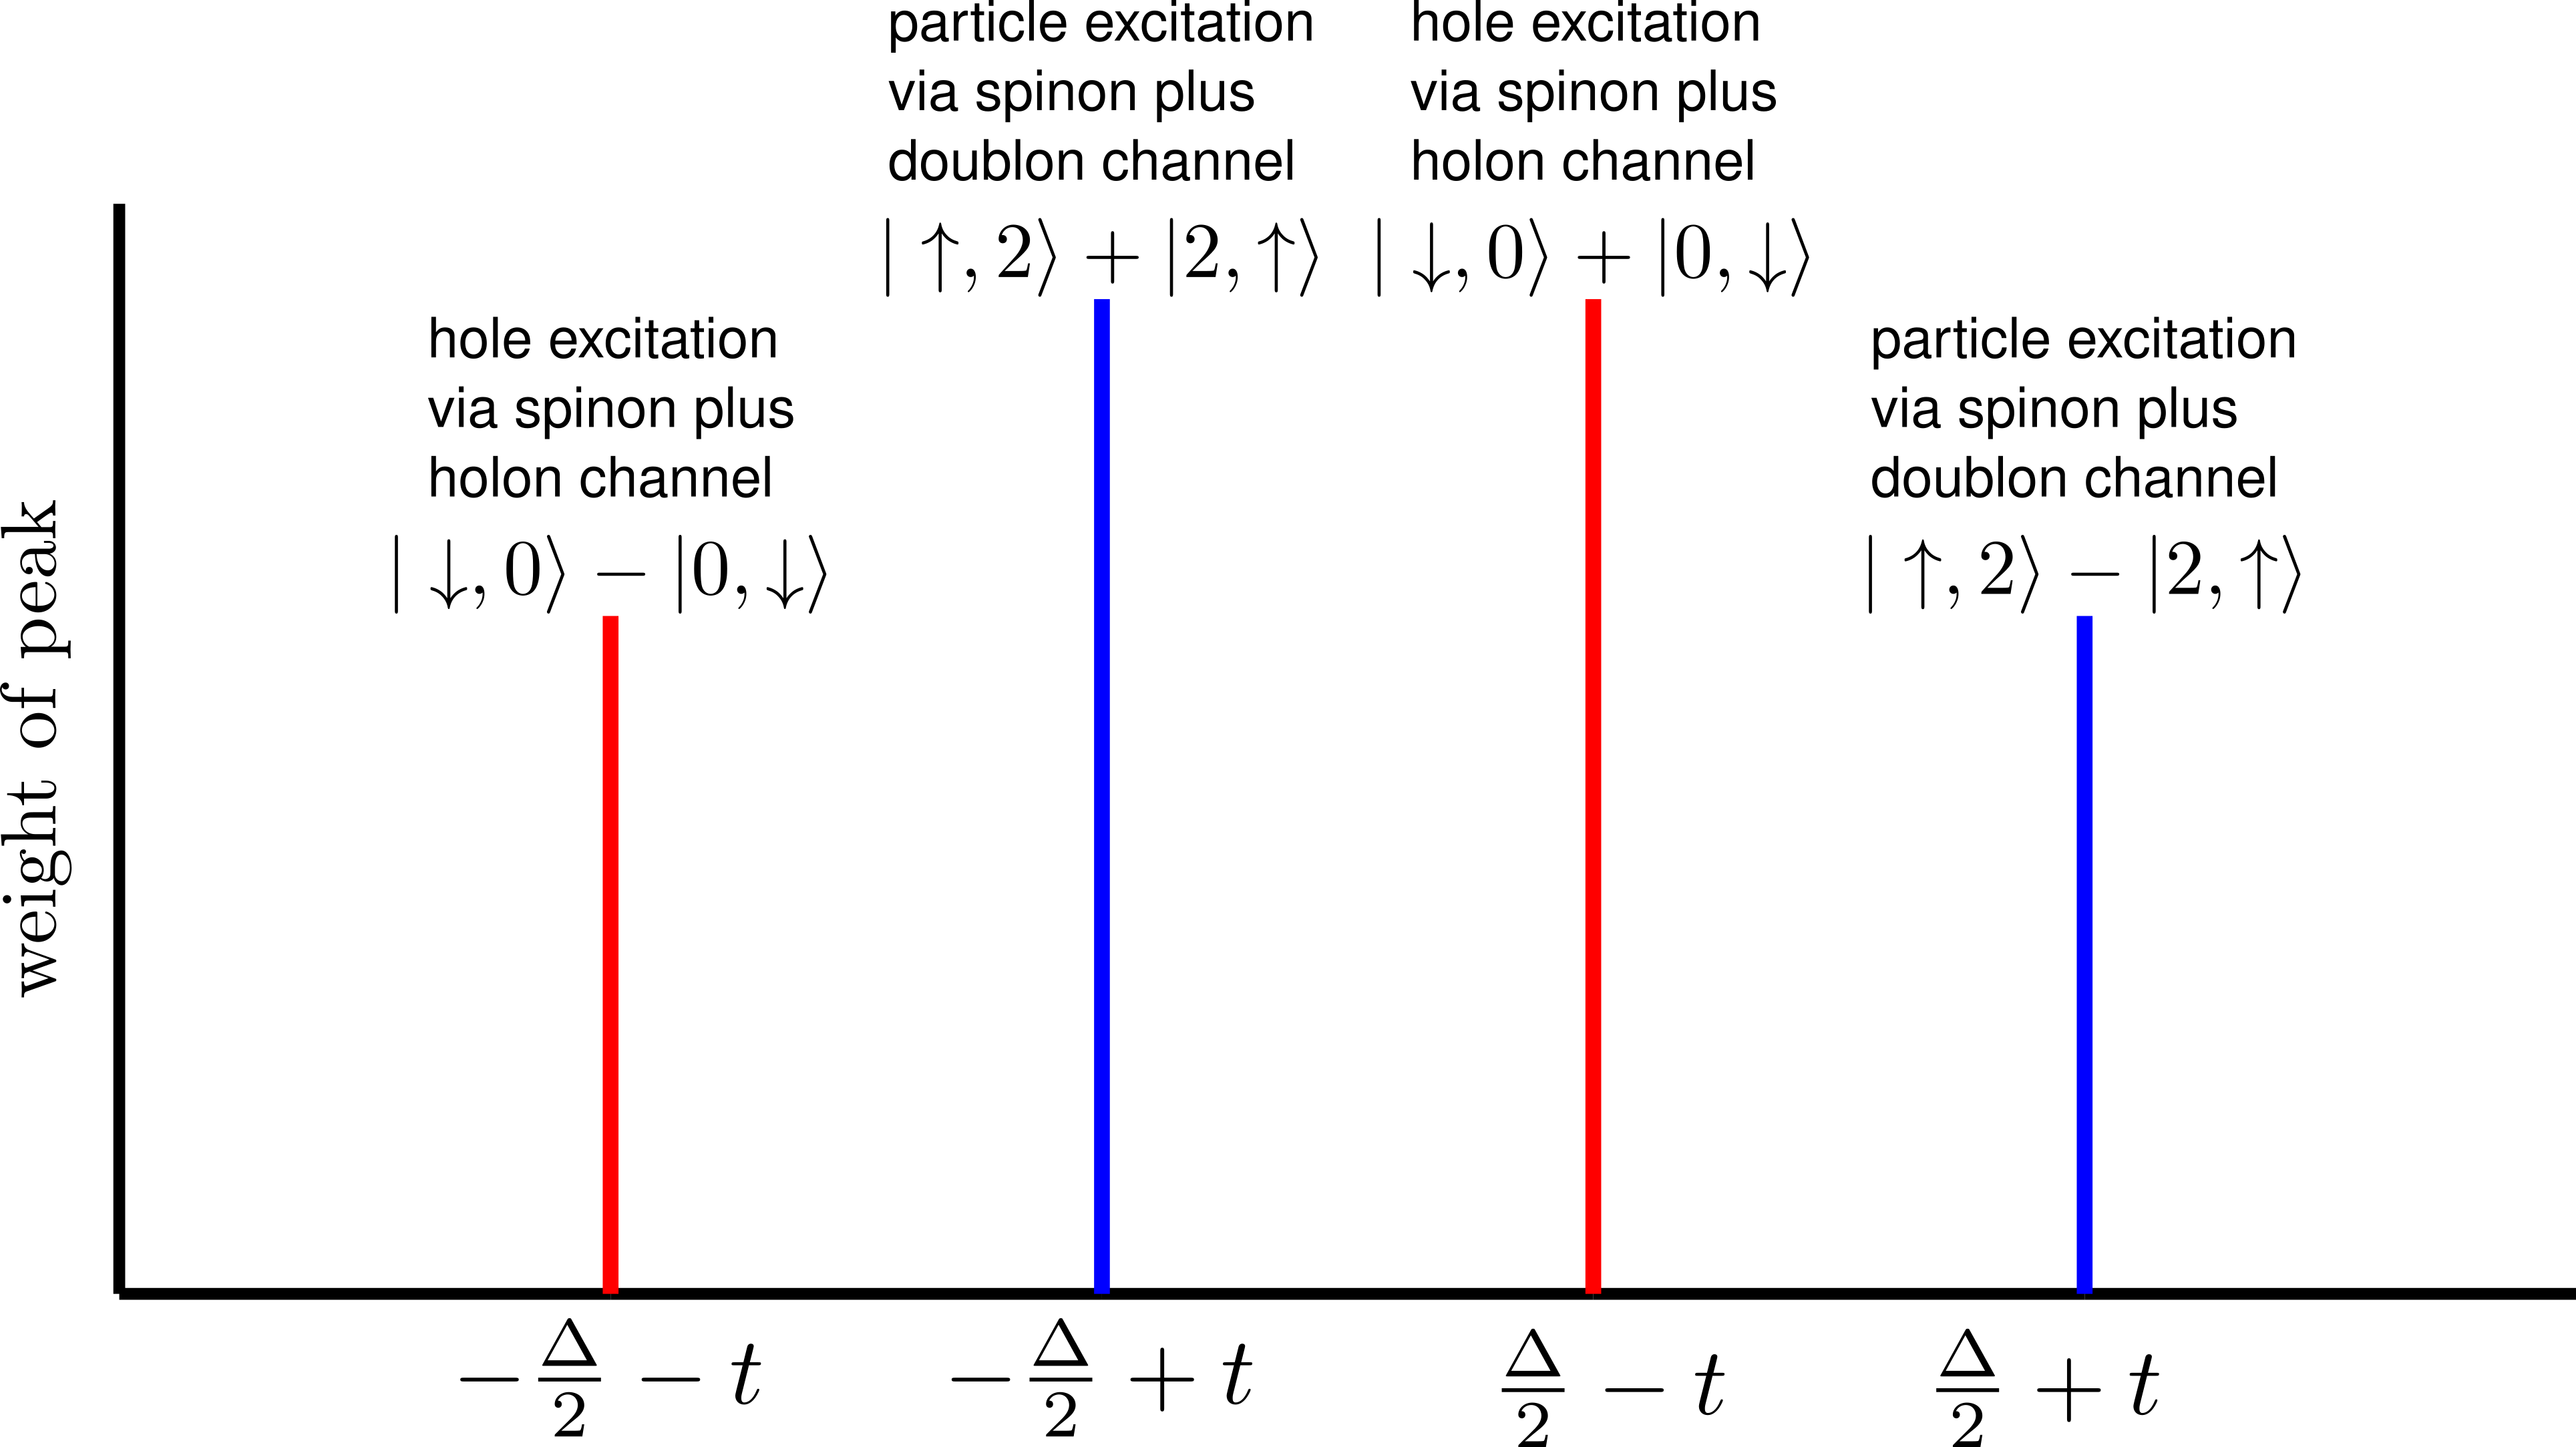
\includegraphics[width=0.9\textwidth]{../figures/dimer-peaks.png}
	\caption{Position, weight and nature of each of the peaks in the Hubbard dimer site local spectral function}
\end{figure}

\chapter{Simple results for the Greens functions}
\section{Relation between single-particle Greens function and the Greens operator $(T=0)$}
 The single-particle Greens function is defined as the solution of the equation:
 \begin{equation}\begin{aligned}
	 \left(i\partial_t - H(\vec r)\right)G(\vec r,\vec r^\prime, t) = \delta(\vec r - \vec r^\prime)
 \end{aligned}\end{equation}
 and is given by the expression
 \begin{equation}\begin{aligned}
	 G(\vec r,\vec r^\prime, t) = -i \theta(t) \left< \left\{ c(\vec r, t) c^\dagger(\vec r^\prime, 0)\right\} \right>
 \end{aligned}\end{equation}
 This solution can be written in the Lehmann-Kallen representation  and at $T=0$ as
 \begin{equation}\begin{aligned}
	 G(\vec r \sigma, \vec r^\prime \sigma, \omega) = \sum_{n}\left[\frac{\bra{GS}c({\vec r,\sigma})\ket{n}\bra{n}c^\dagger(\vec r^\prime,\sigma)\ket{GS}}{\omega + E_{GS} - E_n} + \frac{\bra{GS}c^\dagger(\vec r^\prime,\sigma)\ket{n}\bra{n}c({\vec r,\sigma})\ket{GS}}{\omega + E_n - E_{GS}}\right]
 \end{aligned}\end{equation}
 The sum is over the exact eigenstates of the Hamiltonian. In what follows, we will represent $\vec r,\sigma \equiv \nu$ and $\vec r^\prime,\sigma \equiv \nu^\prime$.
 \begin{equation}\begin{aligned}
	 G(\nu, \nu^\prime, \omega) &= \sum_{n}\left[\frac{\bra{GS}c(\nu)\ket{n}\bra{n}c^\dagger(\nu^\prime)\ket{GS}}{\omega + E_{GS} - E_n} + \frac{\bra{GS}c^\dagger(\nu^\prime)\ket{n}\bra{n}c(\nu)\ket{GS}}{\omega + E_n - E_{GS}}\right]\\
							&= \bra{GS}c(\nu)\frac{1}{\omega + E_{GS} - H}c^\dagger(\nu^\prime)\ket{GS} + \bra{GS}c^\dagger(\nu^\prime)\frac{1}{\omega + H - E_{GS}}c(\nu)\ket{GS}\\
 \end{aligned}\end{equation}
 If we now define a Greens operator
 \begin{equation}\begin{aligned}
	 \label{inv_G_func}
	 \mathcal{G}(\omega, H) = \frac{1}{\omega - (H - E_\text{GS})}
 \end{aligned}\end{equation}
 we can write the single-particle Greens function as a sum of the matrix elements of this operator:
 \begin{equation}\begin{aligned}
	 \label{G_mat_el}
	 G(\nu, \nu^\prime, \omega) = \bra{\nu} \mathcal{G}(\omega, H) \ket{\nu^\prime} - \bra{\overline{\nu^\prime}} \mathcal{G}(-\omega, H) \ket{\overline\nu} = \mathcal{G}(\omega, H)_{\nu,\nu^\prime} - \mathcal{G}(-\omega, H)_{\overline{\nu^\prime}, \overline\nu}
 \end{aligned}\end{equation}
 where we have defined the states $\ket{\nu} \equiv c^\dagger(\nu)\ket{GS}$ and $\ket{\overline\nu} \equiv c(\nu)\ket{GS}$. The two matrix elements can also be represented in their individual spectral representations:
 \begin{equation}\begin{aligned}
	 \label{G_mat_spec}
 	\mathcal{G}(\omega, H)_{\nu,\nu^\prime} = \sum_{n}\frac{\bra{GS}c(\nu)\ket{n}\bra{n}c^\dagger(\nu^\prime)\ket{GS}}{\omega + E_{GS} - E_n}\\
	\mathcal{G}(\omega, H)_{\overline{\nu^\prime}, \overline\nu} = \sum_{n}\frac{\bra{GS}c^\dagger(\nu^\prime)\ket{n}\bra{n}c(\nu)\ket{GS}}{\omega + E_\text{GS} - E_n}
 \end{aligned}\end{equation}
 
\section{Writing single-particle excitations of ground state in terms of $N=3, S^z = \frac{1}{2}$ eigenstates}
The excited state $c^\dagger_{0\uparrow}\ket{\text{GS}}$ can actually be written in terms of the $N=3$, $S^z = + \frac{1}{2}$ eigenstates $\ket{3\pm\uparrow}$ defined in table \ref{hubb_dim_spectrum}.
\begin{equation}\begin{aligned}
	\ket{3\pm \uparrow} = \frac{1}{\sqrt 2}\left(\ket{\uparrow, 2} \pm \ket{2, \uparrow}\right), && H^D \ket{3\pm \uparrow} = \pm t\ket{3\pm \uparrow}
\end{aligned}\end{equation}
In terms of these eigenstates, we can write
\begin{equation}\begin{aligned}
	c^\dagger_{0\uparrow}\ket{\text{GS}} 
	&= c^\dagger_{0\uparrow}\left[a_1 \ket{SS} + a_2 \ket{CT}\right] \\
	&= a_2 \frac{1}{\sqrt 2}\ket{\uparrow,2} - a_1 \frac{1}{\sqrt 2}\ket{2, \uparrow}\\
	&= \left(x + y\right) \frac{1}{\sqrt 2}\ket{\uparrow,2} + \left(x - y\right) \frac{1}{\sqrt 2}\ket{2, \uparrow}\\
	&=x\ket{3+ \uparrow} + y\ket{3- \uparrow}
\end{aligned}\end{equation}
where $x + y \equiv a_2$ and $x-y \equiv -a_1$. Similarly, for the other site excitation, we can write
\begin{equation}\begin{aligned}
	c^\dagger_{1\uparrow}\ket{\text{GS}} 
	&= c^\dagger_{1\uparrow}\left[a_1 \ket{SS} + a_2 \ket{CT}\right] \\
	&= a_2 \frac{1}{\sqrt 2}\ket{2, \uparrow} - a_1 \frac{1}{\sqrt 2}\ket{\uparrow, 2}\\
	&=  \left(x + y\right) \frac{1}{\sqrt 2}\ket{2, \uparrow} + \left(x - y\right) \frac{1}{\sqrt 2}\ket{\uparrow, 2}\\
	&=x\ket{3+ \uparrow} - y\ket{3- \uparrow}
\end{aligned}\end{equation}
Solving for $x$ and $y$ gives
\begin{equation}\begin{aligned}
	x = \frac{a_2 - a_1}{2}, && y = \frac{a_2 + a_1}{2}
\end{aligned}\end{equation}
Similarly, we can also write the single-hole excitation $c_{0 \uparrow}\ket{GS}$ in terms of the $N=1, S^z = -\frac{1}{2}$ eigenstates, $\ket{1\pm \downarrow}$:
\begin{equation}\begin{aligned}
	\ket{1\pm \downarrow} = \frac{1}{\sqrt 2}\left(\ket{\downarrow, 0} \pm \ket{0, \downarrow}\right), && H^D \ket{1\pm \downarrow} = \mp t\ket{1\pm \downarrow}
\end{aligned}\end{equation}
\begin{equation}\begin{aligned}
	c_{0 \uparrow}\ket{GS} = a_1 \frac{1}{\sqrt 2}\ket{0, \downarrow} + a_2 \frac{1}{\sqrt 2}\ket{\downarrow, 0} = y\ket{1+ \downarrow} + x\ket{1- \downarrow}\\
	c_{1 \uparrow}\ket{GS} = a_1 \frac{1}{\sqrt 2}\ket{\downarrow, 0} + a_2 \frac{1}{\sqrt 2}\ket{0, \downarrow} = y\ket{1+ \downarrow} - x\ket{1- \downarrow}\\
\end{aligned}\end{equation}

\section{Matrix elements of $G^{-1}$ between single-particle momentum excitations, for the Hubbard dimer}
\begin{equation}\begin{aligned}
	G^{-1} \equiv \omega + E_\text{GS} - H_D
\end{aligned}\end{equation}
The particle excitation momentum space kets are $\ket{k_0} = \frac{1}{\sqrt 2}\left(\ket{0} + \ket{1}\right) ,\ket{k_\pi} = \frac{1}{\sqrt 2}\left(\ket{0} - \ket{1}\right)$. Therefore,
\begin{equation}\begin{aligned}
	\left(G^{-1}\right)_{k_0 k_0} &= \frac{1}{2}\left(\bra{0} + \bra{1}\right)\left(\omega + E_\text{GS} - H_D\right)\left(\ket{0} + \ket{1}\right)\\
				      &= \frac{1}{2}\left(2x\bra{+}\right)\left(\omega + E_\text{GS} - H_D\right)\left(2x\ket{+}\right)\\
				      &= 2x^2\left(\omega + E_\text{GS} - t\right)\\
\end{aligned}\end{equation}
At the final step, we used $\braket{+,+} = 1$ and $\braket{+|H_D|+} = t$.

\chapter{Topological interpretation of the Wilson ratio}
From the Friedel sum rule\cite{langer1961friedel}, we can relate the phase shift \(\delta(0)\) due to scattering (at the Fermi surface) off a local impurity to the number of electrons bound in the potential well produced by that impurity:
\begin{equation}\begin{aligned}
\widetilde N = \frac{1}{2\pi i}\text{Tr }\ln S(0) = \int_\Gamma dz\partial_z \frac{1}{2\pi i}\text{Tr }\ln S(0)
\end{aligned}\end{equation}
From the optical theorem, we can write
\begin{equation}\begin{aligned}
	S = 1 + TG_0 = \frac{G}{G_0} && \left[G = G_0 + G_0 T G_0\right]
\end{aligned}\end{equation}
This allows us to write \cite{anirbanurg1}
\begin{equation}\begin{aligned}
\widetilde N = \int_\Gamma dz\partial_z \frac{1}{2\pi i}\text{Tr }\ln \frac{G}{G_0}
\end{aligned}\end{equation}
Since \(\text{Tr }\ln \hat O = \sum_\lambda \ln O_\lambda = \ln \prod_\lambda O_\lambda = \ln \text{Det} \hat O\), we get
\begin{equation}\begin{aligned}
\widetilde N &= \int_\Gamma dz\partial_z \frac{1}{2\pi i}\ln \text{Det } \frac{G}{G_0}\\
      &= -\int_\Gamma dz\partial_z \frac{1}{2\pi i}\ln \frac{\text{Det } G_0}{\text{Det } G}\\
      &\equiv -\int_\Gamma dz\partial_z \frac{1}{2\pi i}\ln D\\
      &= -\int_{\Gamma(D)}\frac{dD}{D}
\end{aligned}\end{equation}
From the work of Seki and Yunoki \cite{seki2017topological}, we know that this quantity is essentially the winding number of the curve \(\Gamma(D)\) in the complex plane spanned by the real and imaginary parts of \(D\), and is equal to the change in Luttinger's volume \(V_L\) at \(T=0\).
\begin{equation}\begin{aligned}
\widetilde N &= -\int_{\Gamma(D)}\frac{dD}{D} = -\Delta V_L
\end{aligned}\end{equation}
The incoming electrons can have \(\sigma = \uparrow,\downarrow\).
Since the impurity singlet ground state is rotationally invariant, we have \(\delta_\uparrow = \delta_\downarrow = \delta(0)\).
\begin{equation}\begin{aligned}
\widetilde N &= \frac{1}{\pi}\sum_\sigma\delta_\sigma(0)\\
\implies \delta(0) &= \frac{\pi}{2}\widetilde N = -\frac{\pi}{2}\Delta V_L
\end{aligned}\end{equation}
\begin{equation}\begin{aligned}
\label{wilson_luttinger}
R &= 1 + \sin^2 \left(\frac{\pi}{2}\widetilde N\right)\\
  &= 1 + \sin^2 \left(\frac{\pi}{2}\Delta V_L\right)
\end{aligned}\end{equation}
We note that this connection between \(R\) and \(\Delta V_L\) has not been obtained in the existing literature thus far. In the unitary limit, \(\delta(0) = \frac{\pi}{2}\), giving \(\Delta V_L = -1 = -\tilde N\) \cite{martin1982fermi} (i.e., one electronic state from the impurity has been absorbed into the Luttinger volume of the conduction bath), such that \(R = 2\) in this limit. In this way, we see that a change in the topological quantum number \(\tilde N\) causes the well known renormalisation of the Wilson ratio R from its non-interacting value \((1)\) to the value \((2)\) obtained for the local Fermi liquid \cite{nozieres1974fermi}.

\chapter{Physics of the generalised single-impurity Anderson model}
\label{chap:urg1}
\section{Introduction of spin-exchange and charge isospin-exchange interactions into the SIAM: the generalised SIAM}
We will now study the generalised SIAM obtained by introducing spin-exchange and charge isospin-exchange interactions between the impurity and the conduction bath~\cite{zitko_2006}. Such terms are generated when one does a Schrieffer-Wolff transformation on the SIAM, but we will find it prudent to keep these terms in the bare model itself.

The spin-exchange interaction has the form
\begin{equation}\begin{aligned}
	J \vec{S_d}\cdot\vec{s} = J \left[S_d^z s^z + \frac{1}{2}\left( S_d^+ s^- + S_d^- s^+ \right) \right] ~,
\end{aligned}\end{equation}
where \(\vec S_d = \left(S_d^x, S_d^y, S_d^z\right) = \sum_{\alpha\beta}\vec \sigma_{\alpha\beta}c^\dagger_{d\alpha}c_{d\beta}\) is the impurity spin operator, \(\vec s = \sum_{kk^\prime\alpha\beta}\vec \sigma_{\alpha\beta}c^\dagger_{k\alpha}c_{k^\prime\beta}\) is the spin operator for the conduction bath and \(J\) is the spin-exchange coupling. The bath spin operator actually acts locally, as can be seen by Fourier transforming to real space (using the definition \(f(k) = \frac{1}{\sqrt N}\sum_r g(r)\exp(ikr)\)):
\begin{equation}\begin{aligned}
	\vec s = \sum_{k k^\prime r r^\prime} \frac{1}{N} e^{ikr - ik^\prime r^\prime} \vec \sigma_{\alpha\beta} c^\dagger_{r\alpha} c_{r^\prime\beta} = \sum_{rr^\prime}\frac{1}{N}\vec \sigma_{\alpha\beta} c^\dagger_{r\alpha} c_{r^\prime\beta} N \delta(r)\delta(r^\prime) = \vec \sigma_{\alpha\beta} c^\dagger_{0\alpha} c_{0\beta}
\end{aligned}\end{equation}

In order to introduce the charge isospin coupling, we define the Nambu spinor \cite{anderson1958random,nambu_1960} \(\psi^k = \left( c_{k\uparrow} \quad c^\dagger_{k\downarrow} \right)\), and the charge isospin \cite{zitko_2006} for the mobile conduction electrons
\begin{equation}\begin{aligned}
\vec C = \sum_{kk^\prime} {\psi^k}^\dagger \vec S \psi^{k^\prime} = \frac{1}{2}\sum_{kk^\prime\alpha\beta} {\psi^k_\alpha}^\dagger \vec \sigma_{\alpha\beta} \psi^{k^\prime}_\beta
\end{aligned}\end{equation}
The various components of the isospin are
\begin{equation}\begin{aligned}
	C^z &= \sum_{kk^\prime\sigma}\frac{1}{2} {\psi^k_\sigma}^\dagger \sigma^z_{\sigma\sigma} \psi^{k^\prime}_\sigma = \frac{1}{2}\sum_{kk^\prime\sigma}\left(c^\dagger_{k\sigma}c_{k^\prime \sigma} - \frac{1}{2}\delta_{kk^\prime}\right)\label{diagonalCz}\\
	C^x &= \sum_{kk^\prime\sigma}\frac{1}{2} {\psi^k_\sigma}^\dagger \sigma^x_{\sigma\overline\sigma} \psi^{k^\prime}_{\overline\sigma} = \sum_{kk^\prime\sigma} \frac{\sigma}{4}\left( c^\dagger_{k\sigma}c^\dagger_{k^\prime\overline\sigma} + \text{h.c.} \right) \\
	C^y &= \sum_{kk^\prime\sigma}\frac{1}{2} {\psi^k_\sigma}^\dagger \sigma^y_{\sigma\overline\sigma} \psi^{k^\prime}_{\overline\sigma} = \sum_{kk^\prime\sigma} - \frac{i\sigma}{4}\left( c^\dagger_{k\sigma}c^\dagger_{k^\prime\overline\sigma} - \text{h.c.} \right)\\
\end{aligned}\end{equation}
It is easy to verify that these operators satisfy the SU(2) commutation algebra. For example, if we write \(C^x = A + A^\dagger\) and \(C^y = B + B^\dagger\), then \(\left[ C^x, C^y \right] = \left[ A, B^\dagger \right] - \text{h.c.}\), where
\begin{equation}\begin{aligned}
	\left[ A, B^\dagger \right] = \frac{1}{4}\sum_{kk^\prime,qq^\prime}\left[ c^\dagger_{k\uparrow}c^\dagger_{k^\prime \downarrow}, i c_{q^\prime \downarrow}c_{q \uparrow} \right] = \frac{i}{4}\sum_{kq}\left(c^\dagger_{k\uparrow}c_{q \uparrow} - c_{k \downarrow}c^\dagger_{q \downarrow}\right)
\end{aligned}\end{equation}
and therefore
\begin{equation}\begin{aligned}
	\implies \left[ C^x, C^y \right] = \frac{i}{2}\sum_{kq}\left(c^\dagger_{k\uparrow}c_{q \uparrow} - c_{k \downarrow}c^\dagger_{q \downarrow}\right) = i C^z
\end{aligned}\end{equation}
There are similar operators for the impurity electron:
\begin{equation}\begin{aligned}
	\psi_d = \left( c_{d\uparrow} \quad c^\dagger_{d\downarrow}\right), &&\vec C_d = \frac{1}{2}\sum_{\beta} {\psi_{d,\alpha}}^\dagger \vec \sigma_{\alpha\beta} \psi_{d,\beta}
\end{aligned}\end{equation}
The full charge-Kondo interaction can now be written down in terms of these isospins:
\begin{equation}\begin{aligned}
	K \vec{C_d}\cdot\vec{C} = K \left[C_d^z C^z + \frac{1}{2}\left(C_d^+ C^-+ C_d^- C^+\right)\right]
\end{aligned}\end{equation}
where \(C^\pm \equiv C^x \pm iC^y\).
\begin{equation}\begin{aligned}
	C^+ = \sum_{kk^\prime} c^\dagger_{k\uparrow}c^\dagger_{k^\prime\downarrow}, && C^- = \sum_{kk^\prime}c_{k^\prime\downarrow}c_{k\uparrow}
\end{aligned}\end{equation}
The full generalised Anderson model Hamiltonian, at particle-hole symmetry, is
\begin{equation}\begin{aligned}
	\mathcal{H} = \sum_{k\sigma}\epsilon_k \tau_{k\sigma} + \epsilon_d \left( \hat n_{d \uparrow} - \hat n_{d \downarrow} \right) ^2 + \sum_{k\sigma} \left(V_{k} c^\dagger_{k\sigma} c_{d\sigma} + h.c.\right) +J \vec{S_d}\cdot\vec{s} + K \vec{C_d}\cdot\vec{C}
\end{aligned}\end{equation}

For the URG analysis, at each RG step, we decouple the electronic states \(q\beta\) on the \(k-\)space shell of radius\(\Lambda_j\). For simplicity, we will only consider those diagonal terms in the denominator that either have both \(q\beta\) and \(q\overline\beta\) or  both \(q\beta\) and \(d\) or both \(q\overline\beta\) and \(d\). Terms that have purely \(q\overline\beta\) will not be considered. Also, the scattering between just \(d\) and \(q\overline\beta\) can be ignored since it is diagonal in \(q\beta\). 
The diagonal (number-preserving) part is
\begin{equation}\begin{aligned}
	H_D = \sum_\beta\epsilon_q\tau_{q\beta} + \epsilon_d \left( \hat n_{d \uparrow} - \hat n_{d \downarrow} \right) ^2 + J S^z_ds^z_{q} + K C^z_d C^z_q\\
\end{aligned}\end{equation}
where \(s_q^z = \frac{1}{2}\left(\hat n_{q\uparrow} - \hat n_{q\downarrow}\right)\) and \(C_q^z = \frac{1}{2}\left(\hat n_{q \uparrow} + \hat n_{q \downarrow} - 1\right)\). The off-diagonal part is:
\begin{equation}\begin{aligned}
	H_X = \sum_{\beta=\uparrow,\downarrow}\left[V c^\dagger_{d\beta}c_{q\beta} + \frac{1}{2}J \sum_{k<\Lambda_N}\left\{\left(\hat n_{d \beta} - \hat n_{d \overline\beta}\right) \frac{1}{2} c^\dagger_{k\beta}c_{q\beta} + c^\dagger_{d\beta}c_{d\overline\beta}c^\dagger_{k\overline\beta}c_{q \beta}\right\} + \frac{1}{2}K \sum_{k<\Lambda_N}\left\{\left(\hat n_d -1\right)\frac{1}{2}c^\dagger_{k\beta}c_{q\beta} + \right.\right.\\
\left.\left.c^\dagger_{d\beta}c^\dagger_{d\overline\beta}c_{k\overline\beta}c_{q\beta}\right\}\right] + \text{h.c.}~.
\end{aligned}\end{equation}

\begin{figure}[!htb]
	\centering
	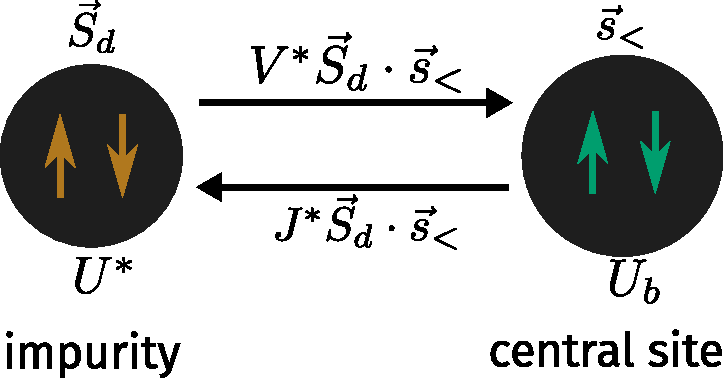
\includegraphics[width=0.5\textwidth]{../figures/zeromode.pdf}
	\caption{While we have studied the full model under renormalisation group, often we will turn to a simplified zero-bandwidth version of the model that is obtained by ignoring the kinetic energy part of the Hamiltonian. This zero-bandwidth model is effectively a two site model.}
\end{figure}

\section{RG equations for generalised SIAM}
\begin{equation}\begin{aligned}
	\Delta \epsilon_d &= 2V^2 n_j\left(\frac{1}{\omega - \frac{D}{2} + \epsilon_d + \frac{K}{4}} - \frac{1}{\omega - \frac{D}{2} - \epsilon_d + \frac{J}{4}}\right) + \frac{n_j}{2}\left(\frac{J^2}{\omega - \frac{D}{2} + \frac{J}{4}} - \frac{K^2}{\omega - \frac{D}{2} + \frac{K}{4}}\right),\\
	\Delta V &= -\frac{3n_j V}{8}\left[J\left(\frac{1}{\omega - \frac{D}{2} + \frac{J}{4}} + \frac{1}{\omega - \frac{D}{2} - \epsilon_d + \frac{J}{4}}\right) + K \left(\frac{1}{\omega - \frac{D}{2} + \frac{K}{4}} + \frac{1}{\omega - \frac{D}{2} + \epsilon_d + \frac{K}{4}}\right)\right],\\
	\Delta J &= -\frac{n_j J^2}{\omega - \frac{D}{2} + \frac{J}{4}},\\ 
	\Delta K &= -\frac{n_j K^2}{\omega - \frac{D}{2} + \frac{K}{4}}
\end{aligned}\end{equation}
In terms of \(U = -2\epsilon_d\), the equations become
\begin{gather}
	\Delta U = 4V^2 n_j\left(\frac{1}{d_1} - \frac{1}{d_0}\right) - n_j\left(\frac{J^2}{d_2} - \frac{K^2}{d_3}\right),\\
	\Delta V = -\frac{3n_j V}{8}\left[J\left(\frac{1}{d_2} + \frac{1}{d_1}\right) + K \left(\frac{1}{d_3} + \frac{1}{d_0}\right)\right],\\
	\Delta J = -\frac{n_j J^2}{d_2}, \quad\quad\Delta K = -\frac{n_j K^2}{d_3}
\end{gather}
\(d_i\) are the denominators:
\begin{equation}\begin{aligned}
	\label{denominators}
	d_0 = \omega - \frac{D}{2} - \frac{U}{2} + \frac{K}{4}, \quad d_1 = \omega - \frac{D}{2} + \frac{U}{2} + \frac{J}{4}, \quad d_2 = \omega - \frac{D}{2} + \frac{J}{4}, \quad d_3 = \omega - \frac{D}{2} + \frac{K}{4}
\end{aligned}\end{equation}

\section{Nature of coupling RG flows}
\subsection{Repulsive interaction on impurity: \(U>0\)}
For the Hamiltonians with positive on-site correlation, we will assume that the spin-exchange coupling is positive and charge isospin-exchange coupling is negative: \(J>0, K<0\). This choice is motivated by the signs of the corresponding terms when they are generated via a Schrieffer-Wolff transformation~\cite{schrieffer1966}. The impurity-bath hybridisation \(V\) is always positive. The sign of the couplings lead to inequalities among the denominators which we will utilise at various points. First of all, since \(U>0\), we have \(d_1 - d_2 = \frac{U}{2} > 0\). Secondly, since \(K<0\), we have \(d_2 - d_3 = \frac{J-K}{4} > 0\). And finally, we have \(d_3 - d_0 = \frac{U}{2} > 0\). Combining these, we can write
\begin{equation}\begin{aligned}
	\label{ineq_den}
	d_1 > d_2 > d_3 > d_0
\end{aligned}\end{equation}

The strong coupling regime is defined as the range of values of \(\omega\) where the hybridisation is relevant. This is ensured by the assumption \(d_1<0\). From eq.~\ref{ineq_den}, we can then conclude that all denominators are negative: \(d_i = - |d_i|\). The simplest consequence of this is the RG flow of \(K\):
\begin{equation}\begin{aligned}
	\Delta K= -\frac{n_j K^2}{d_3} = \frac{n_j K^2}{|d_3|} > 0 \implies K_{j+1} > K_j \implies K_0 = -|K_0|, K^* \to 0
\end{aligned}\end{equation}
\(K_j\) is the value of \(K\) after the \(j^\text{th}\) RG step, \(K_0\) representing the bare value.
In other words, since \(d_3 < 0\), the RG equation for \(K\) provides an algebraic increment, and the negative \(K\) increases and flows towards zero. The \(*\) indicates a fixed point value. The isospin coupling is irrelevant in this regime, and we will ignore it.

The coupling \(J\), on the other hand, is relevant and flows from a small positive value towards a large value at strong coupling.
\begin{equation}\begin{aligned}
	\Delta J= -\frac{n_j J^2}{d_2} = \frac{n_j J^2}{|d_2|} > 0 \implies J_{j+1} > J_j \implies J_0 \to \text{ large } J^* ~(\text{strong coupling})
\end{aligned}\end{equation}
The value of \(J^*\) is obtained when the denominator \(d_2\) vanishes.

Because of the RG irrelevance of \(K\), we can simplify the RG equation for \(V\):
\begin{equation}\begin{aligned}
	\Delta V = -\frac{3n_j VJ}{8}\left(\frac{1}{d_2} + \frac{1}{d_1}\right) = \frac{3n_j VJ}{8}\left(\frac{1}{|d_2|} + \frac{1}{|d_1|}\right) > 0
\end{aligned}\end{equation}
Since both the denominators are positive, \(V\) is relevant. The fixed point value \(V^*\) is attained when the denominator \(d_1\) vanishes (\(d_1\) will vanish earlier than \(d_2\)).

We can compare the rate of flows of \(V\) and \(J\):
\begin{equation}\begin{aligned}
	\frac{\Delta V}{\Delta J} = \frac{3V}{8J}\left(1 + \frac{|d_2|}{|d_1|}\right) > \frac{3V}{4J}
\end{aligned}\end{equation}
There we used the fact that \(|d_2| > |d_1|\).
We finally come to the RG equation for \(U\):
\begin{equation}\begin{aligned}
	\Delta U = 4V^2 n_j\left(\frac{1}{d_1} - \frac{1}{d_0}\right) - n_j\frac{J^2}{d_2} = -4V^2\left(U + \frac{J}{4}\right)\frac{n_j}{d_0 d_1} - \frac{n_j J^2}{d_2}
\end{aligned}\end{equation}
For \(V>J\), we can expect \(U\) to be irrelevant. On the other hand, \(V<J\) makes \(U\) relevant.

In short, the \(U>0\) regime is characterised by an irrelevant isospin-exchange coupling \(K\) and a relevant spin-exchange coupling \(J\), and the following set of RG equations for the remaining couplings \(U\) and \(V\):
\begin{equation}\begin{aligned}
	\Delta U = 4V^2 n_j\left(\frac{1}{d_1} - \frac{1}{d_0}\right) - n_j\frac{J^2}{d_2}, \quad \Delta V = -\frac{3n_j VJ}{8}\left(\frac{1}{d_2} + \frac{1}{d_1}\right)
\end{aligned}\end{equation}

\begin{figure}[!htb]
	\centering
	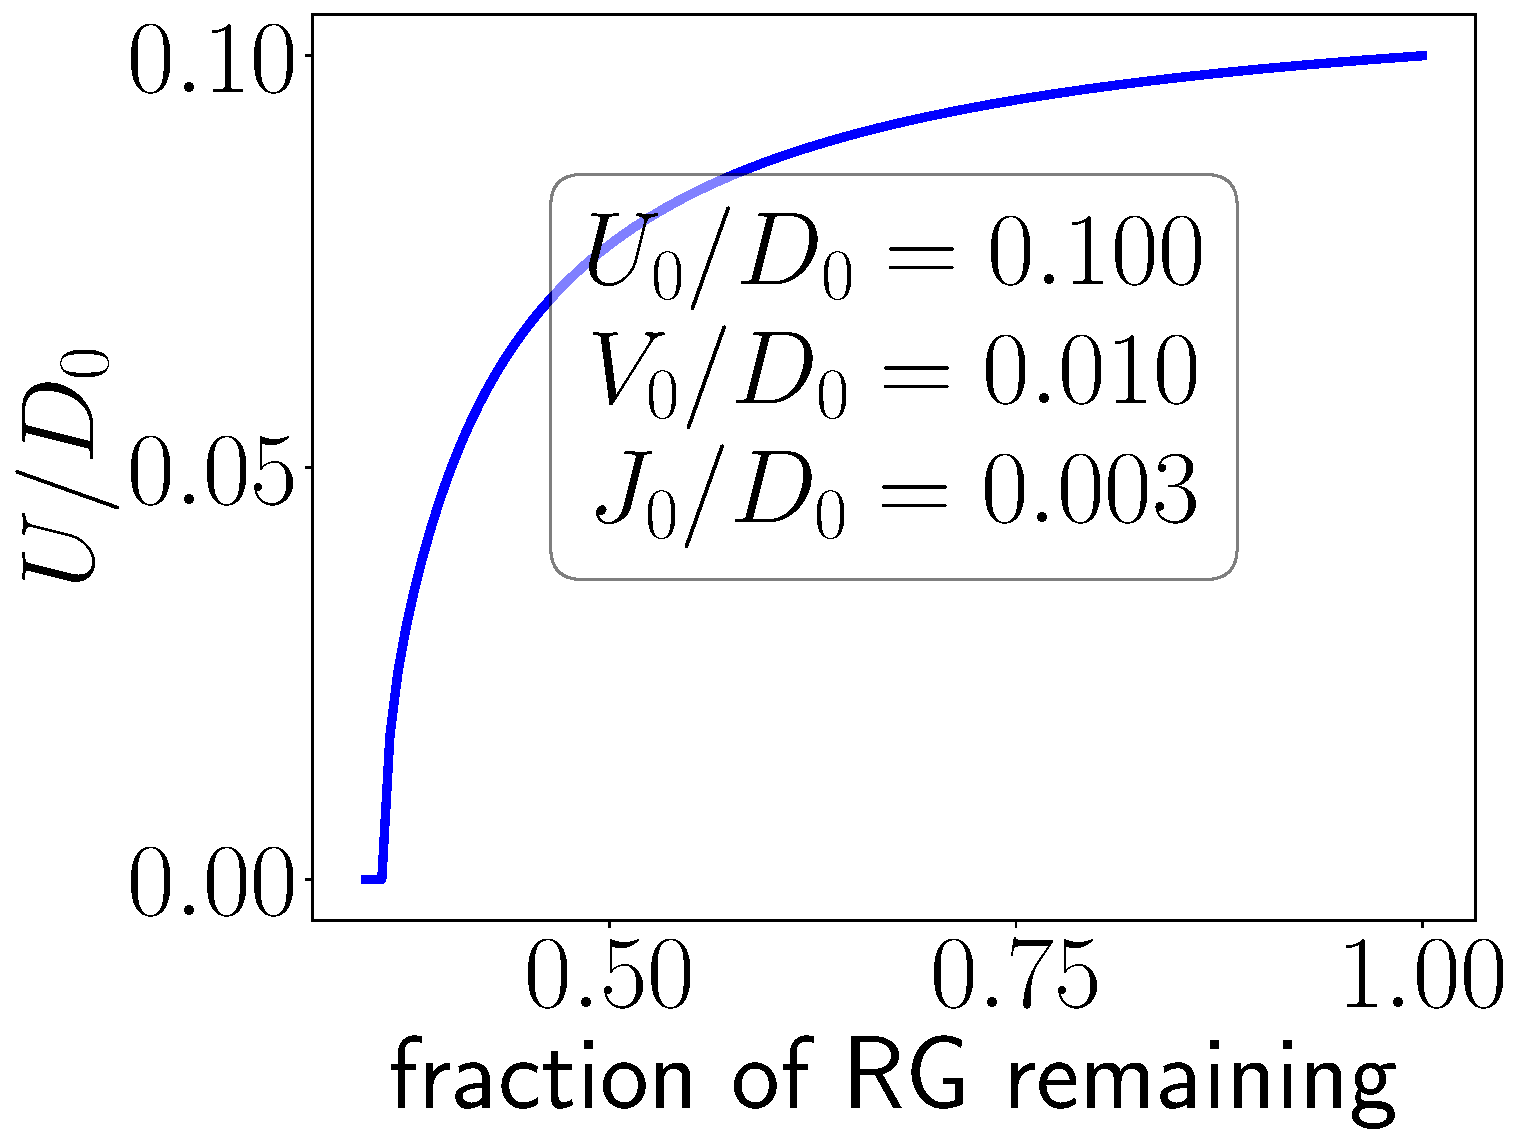
\includegraphics[width=0.32\textwidth]{../figures/U_irr,U_gt_0,U.pdf}
	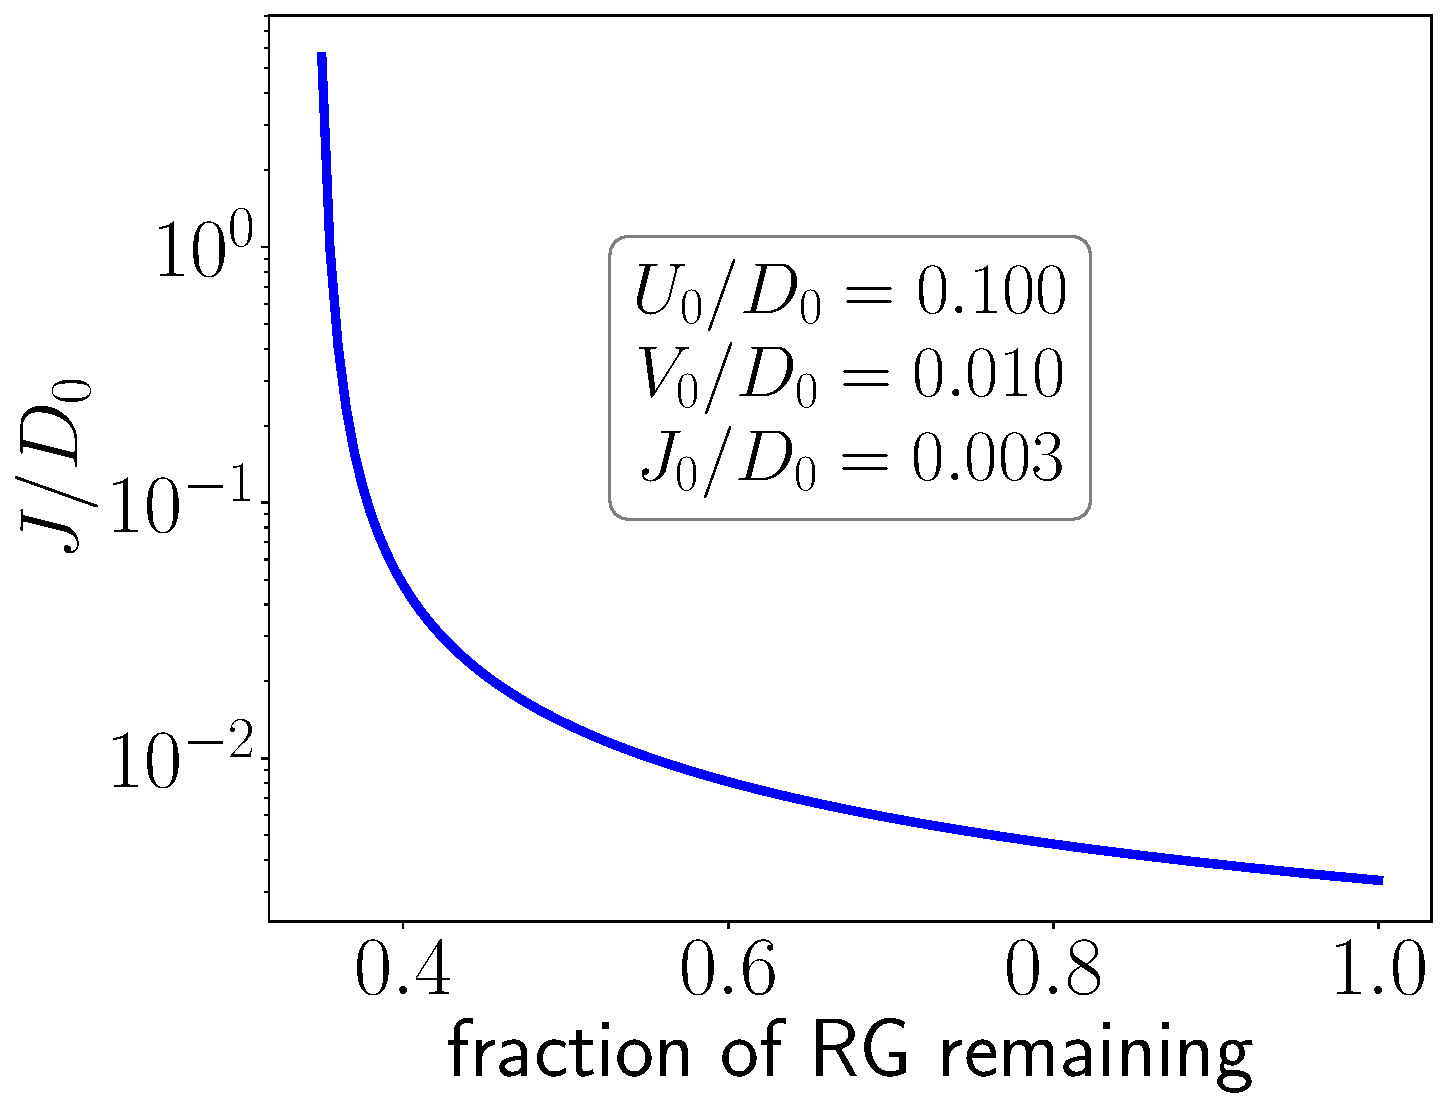
\includegraphics[width=0.32\textwidth]{../figures/U_irr,U_gt_0,J.pdf}
	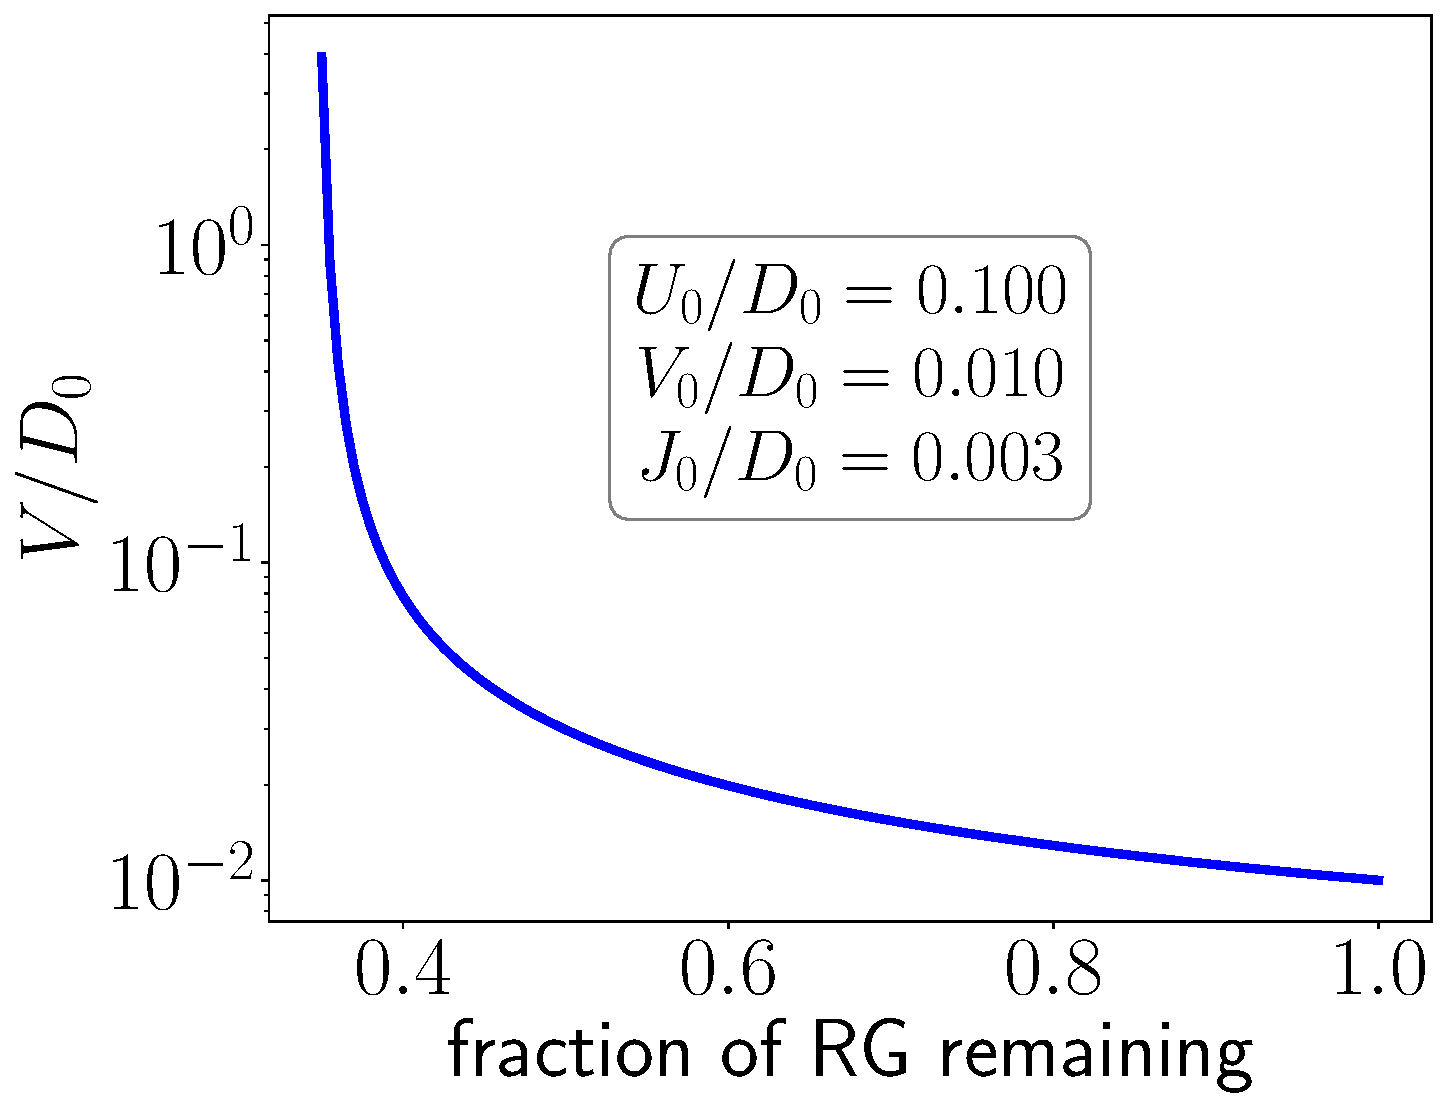
\includegraphics[width=0.32\textwidth]{../figures/U_irr,U_gt_0,V.pdf}
	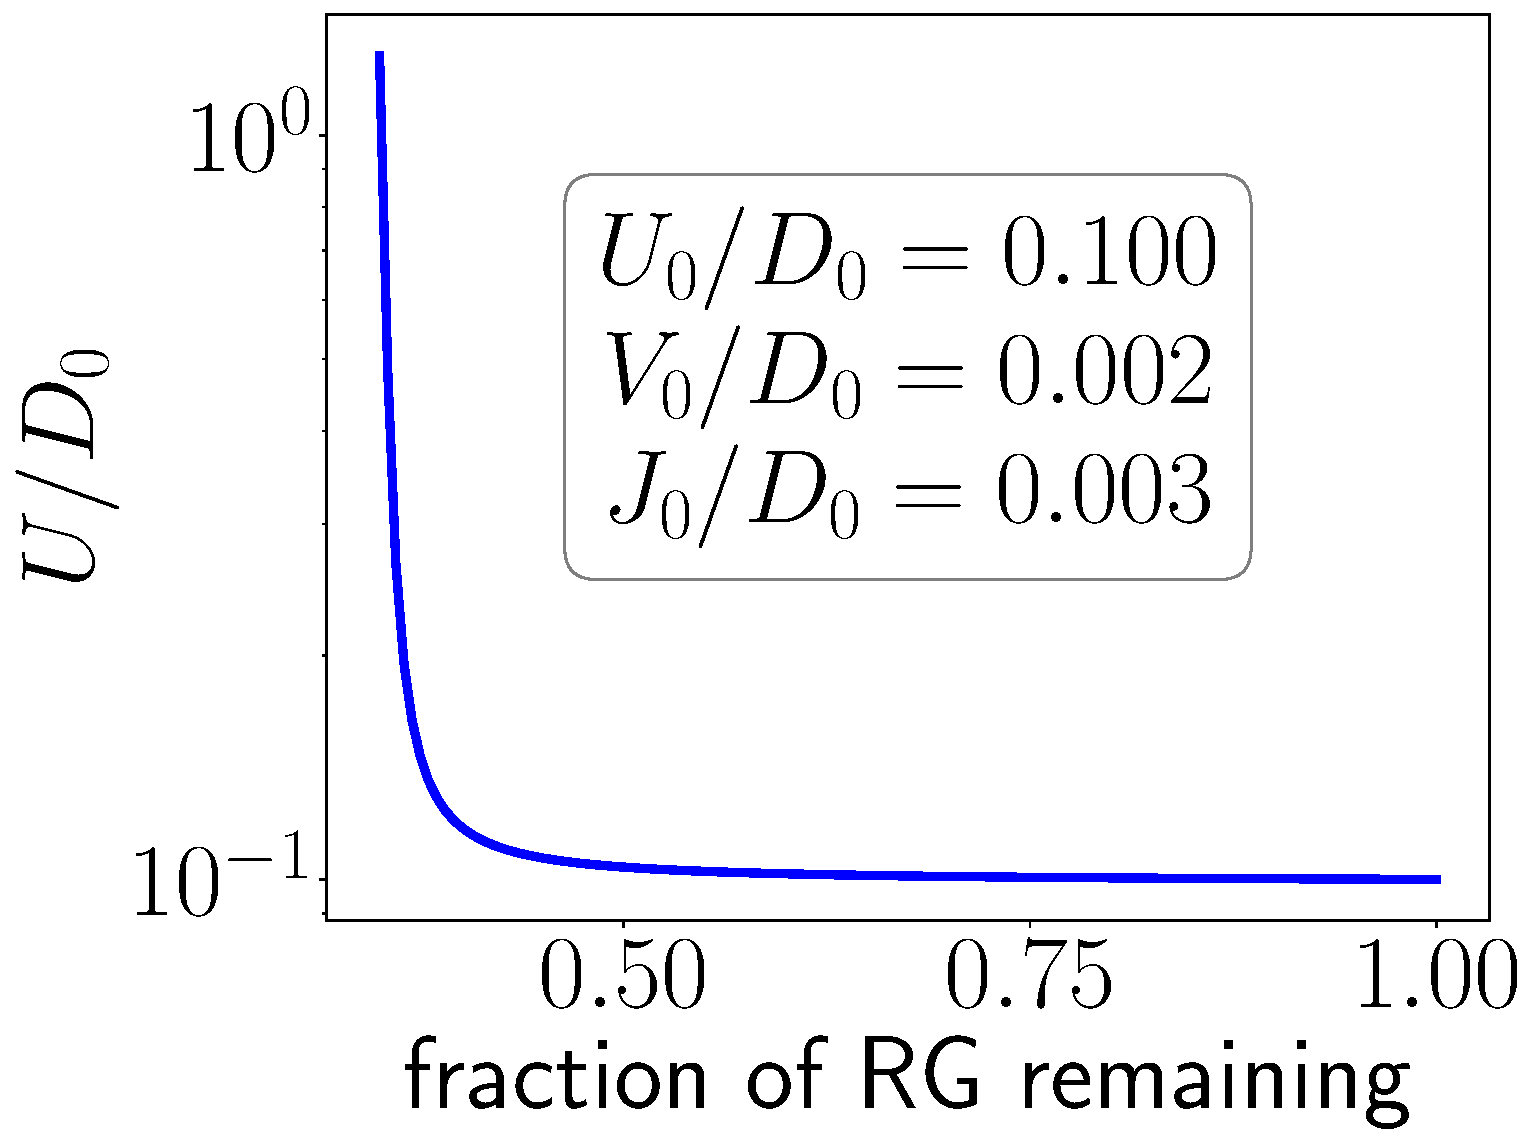
\includegraphics[width=0.32\textwidth]{../figures/U_rel,U_gt_0,U.pdf}
	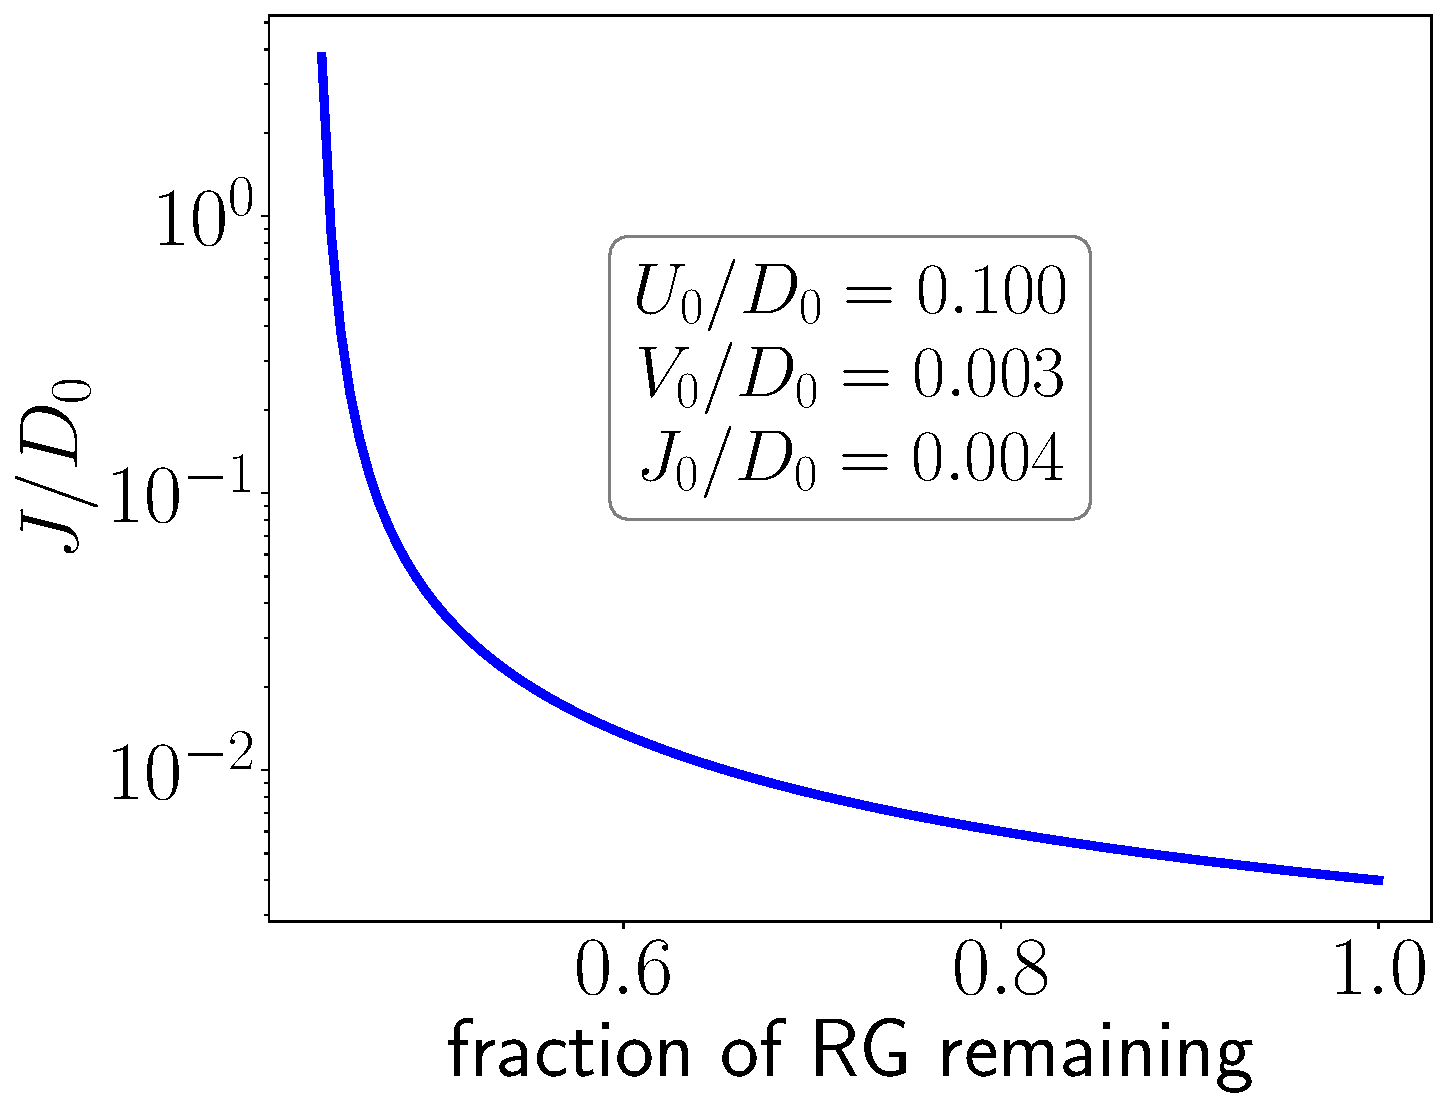
\includegraphics[width=0.32\textwidth]{../figures/U_rel,U_gt_0,J.pdf}
	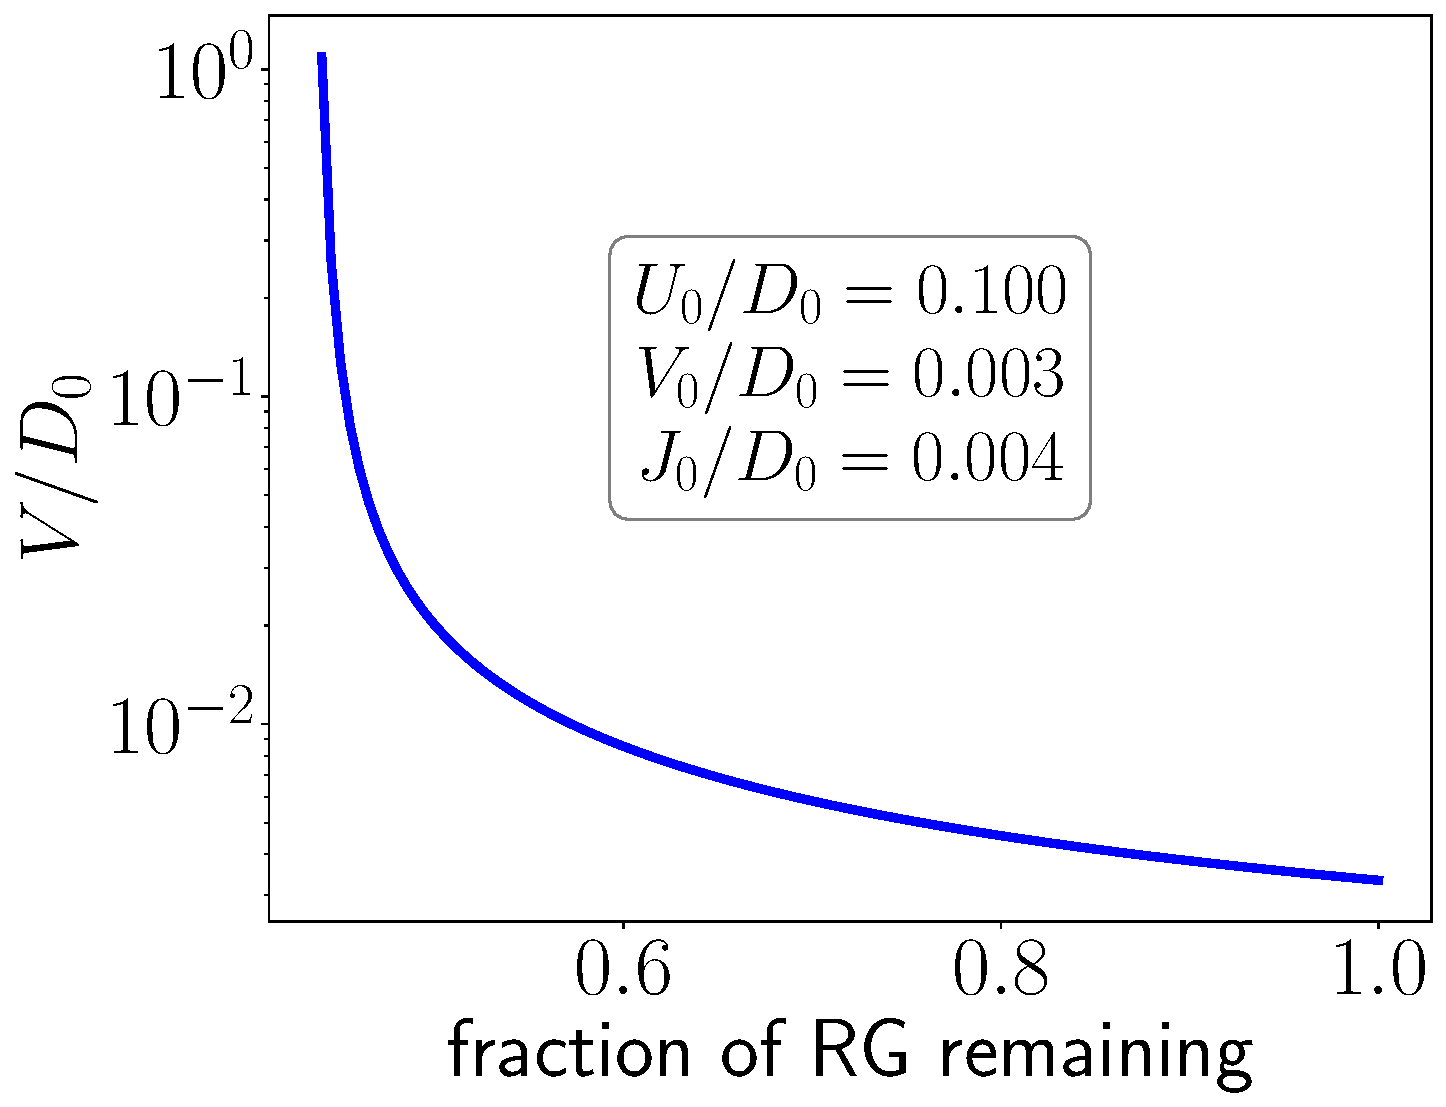
\includegraphics[width=0.32\textwidth]{../figures/U_rel,U_gt_0,V.pdf}
\end{figure}

\subsection{Attractive interaction on impurity: \(U<0\)}
Here, we have \(J<0\) and \(K>0\). The denominators satisfy the following inequality in this regime:
\begin{equation}\begin{aligned}
	d_0 > d_3 > d_2 > d_1
\end{aligned}\end{equation}

The strong coupling regime here corresponds to \(d_0 < 0\). This again means that all the denominators are negative. The spin-exchange coupling \(J\) is now irrelevant, because its bare value is negative while its RG equation is positive: \(\Delta J>0\). Moreover, the isospin coupling \(K\) is now positive and so is its RG equation: \(\Delta K>0\), which means it flows to strong coupling. \(V\) also flows to strong coupling. The RG equation for \(U\) can be written as
\begin{equation}\begin{aligned}
	\Delta U = 4V^2\left(\frac{K}{4} - U\right)\frac{n_j}{d_0 d_1} + \frac{n_j K^2}{d_3}
\end{aligned}\end{equation}
The first term is necessarily positive, while the second term is negative. This means that for roughly \(V_0 > J_0\), we  will have \(\Delta U > 0\), and since \(U_0 < 0\), this amounts to an irrelevant flow of \(U\) towards zero. On the other hand, for \(J_0 > V_0\), we will have \(\Delta U < 0\), and this corresponds to a relevant flow of \(U\) towards large negative value.

In other words, the RG flows in this regime can be exactly mapped to those in the positive \(U\) regime. The general statement is: in the strong coupling regime of positive(negative) \(U\), \(V\) is always relevant, \(J\)(\(K\)) is relevant, \(K\)(\(J\)) is irrelevant, and \(U\) is relevant when \(J(K) > V\), otherwise \(U\) is irrelevant.


\section{Effective Hamiltonian and ground state}
The fixed point Hamiltonian can, in general, be written as
\begin{equation}\begin{aligned}
	\mathcal{H}^* = \sum_{\sigma, k}\epsilon_k \tau_{k\sigma} - \frac{U^*}{2}\left(\hat n_{d \uparrow} - \hat n_{d \downarrow}\right)^2  + \sum_{\sigma, k < \Lambda^*}\left( V^* c^\dagger_{k\sigma}c_{d\sigma} + \text{h.c.} \right) + J^* \vec{S_d}\cdot\vec{s} + K^* \vec{C_d}\cdot\vec{C}
\end{aligned}\end{equation}
The first term is the kinetic energy of all the electrons. The next two terms are the impurity-diagonal pieces, featuring the renormalised interaction \(U^*\). The next three terms are the residual interactions between the impurity and the metal, with the renormalised couplings \(V^*, J^*\) and \(K^*\). The summations in these terms extend from the fixed point momentum cutoff \(\Lambda^*\) to 0. This is the region of momentum space  which the URG was unable to decouple. The operators \(\vec s\) and \(\vec C\) represent the macroscopic magnetic and charge spins formed by the remaining electrons that are lying inside the window \(\left[ 0, \Lambda^* \right] \):
\begin{equation}\begin{aligned}
	\vec s = \sum_{kk^\prime<\Lambda^*\atop{\alpha\beta}} c^\dagger_{k\alpha}\vec \sigma_{\alpha\beta}c_{k^\prime\beta}
\end{aligned}\end{equation}
Our goal here is to write down the ground state wavefunction for this low-energy Hamiltonian.

To make progress, we will simplify the effective Hamiltonian by taking the zero bandwidth limit. This reduces it to a two-site problem. One site is of course the impurity site, and this site will be labeled as site 1. The other site will be formed by the center of mass degree of freedom of the conduction electrons, and will be labeled as site 2. The Hamiltonian for this two-site problem is
\begin{equation}\begin{aligned}
	\mathcal{H}_{IR} = - \frac{U^*}{2}\left(\hat n_{1 \uparrow} - \hat n_{1 \downarrow}\right)^2 + V^*\sum_{\sigma}\left(c^\dagger_{1\sigma}c_{2\sigma} + \text{h.c.} \right) + J^*\vec{S_1}\cdot\vec{S_2} + K^* \vec{C_1}\cdot\vec{C_2}
\end{aligned}\end{equation}
\begin{figure}[!htb]
	\centering
	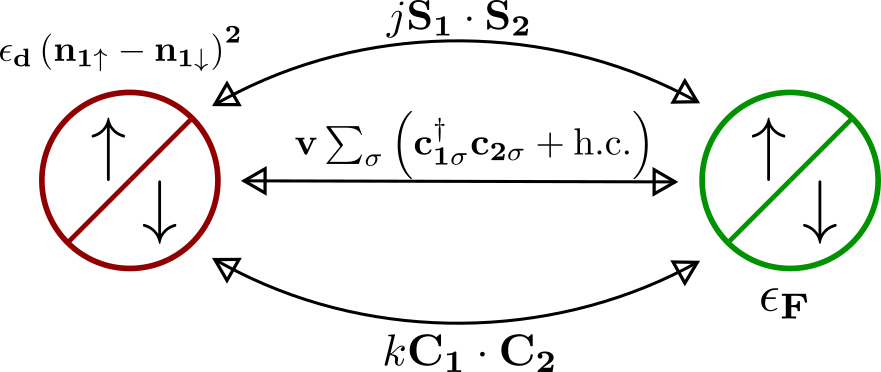
\includegraphics[width=0.4\textwidth]{../figures/two_site_problem.png}
	\caption{Two-site effective problem of fixed point Hamiltonian}
	\label{twosite}

\end{figure}
The subscripts on the operators designate the site on which they act; \(\hat n_1\) is the number operator for the first site.

We will adopt the following notation to represent the states in this Hilbert space. A general state will be represented in the Fock space basis as \(\ket{n_{1 \uparrow}n_{1 \downarrow}n_{2 \uparrow}n_{2 \downarrow}}\). For example,
\begin{equation}\begin{aligned}
	\ket{1101} = c^\dagger_{1 \uparrow}c^\dagger_{1 \downarrow}c^\dagger_{2 \downarrow}\ket{-}
\end{aligned}\end{equation}
\(\ket{-}\) is the vacuum state.

For \(U>0\), the ground state is given by
\begin{gather}
	\label{gstate}
	\ket{\Psi}_\text{1} = c_s \frac{1}{\sqrt 2}\left(\ket{\uparrow, \downarrow} - \ket{\downarrow, \uparrow}\right) + c_c \frac{1}{\sqrt 2}\left(\ket{\uparrow\downarrow, 0} + \ket{0, \uparrow\downarrow}\right), \quad E_1 =  -V^*\sqrt{\gamma^2 + 4} -\frac{1}{4}U^* - \frac{3}{8}{J^*}
\end{gather}
where $\gamma = \frac{1}{2{V^*}}\left[ \frac{1}{4}\left( 3J^* + K^* \right) + \frac{1}{2}U^* \right]$. The probabilities for the spin and charge sectors for the ground state are
\begin{equation}\begin{aligned}
	\label{coeff_def}
	\left(c_s\right)^2 = \frac{1}{2\sqrt{\gamma^2 + 4}}\left(\sqrt{\gamma^2 + 4} + \gamma\right), \quad \left(c_c \right)^2 = \frac{1}{2\sqrt{\gamma^2 + 4}}\left(\sqrt{\gamma^2 + 4} - \gamma\right)~.
\end{aligned}\end{equation}
For (roughly) \(J_0 > V_0\), we get \(J^* \gg V^*\) and \(U^* \gg U_0\) so that \(\gamma \gg 1\). This gives \(\left( c_s \right) ^2 \sim 1\) and \(\left( c_c \right) ^2 \sim 0\). The entire contribution to the ground state then comes from the spin sectors of the two sites. This is calculated numerically in fig.~\ref{cs_cc}.
\begin{figure}[!htb]
	\centering
	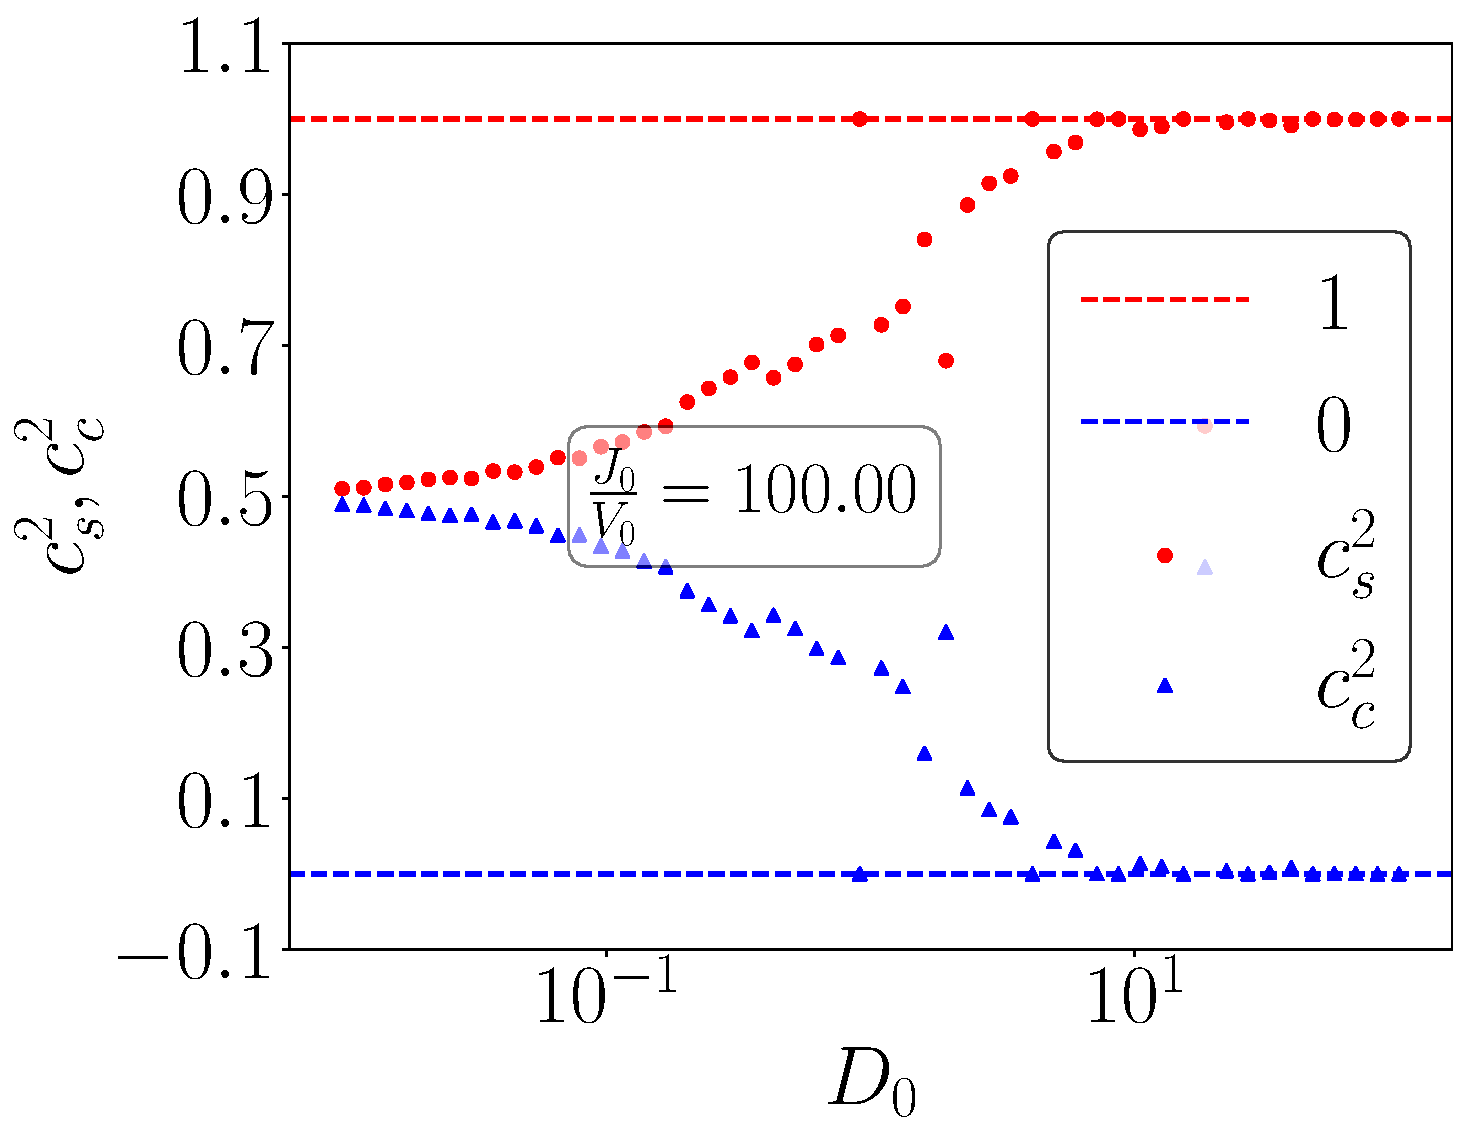
\includegraphics[width=0.8\textwidth]{../figures/coeffs_vs_J.pdf}
	\caption{Variation of relative weights \(c_s\) and \(c_c\) with \(J_0\)}
	\label{cs_cc}
\end{figure}

In the other regime of \(U<0\), the two competing states are \(\ket{\Psi}_1\) defined above (with energy \(E_1\)), and \(\ket{\Psi_2}\), the charge singlet: \(\ket{\Psi}_2 = \frac{1}{\sqrt 2}\left( \ket{2,0} - \ket{0,2} \right)\) having energy \(E_2\).
\begin{equation}\begin{aligned}
	E_2 = -\frac{3}{4}K^*, \quad E_1 - E_2 = -\frac{1}{4}\sqrt{\left( \frac{1}{2}K^* + U^* \right)^2 + (4V^*)^2} - \frac{1}{4}U^* + \frac{3}{4}K^*
\end{aligned}\end{equation}
For \(V_0 \gg K_0\), the largest energy scale will be \(V^*\), and we can then approximate this difference as
\begin{equation}\begin{aligned}
	E_1 - E_2 \simeq -V^* < 0
\end{aligned}\end{equation}
In such a case, \(\ket{\Psi}_1\) will therefore be the ground state. In the other regime \(V_0 \ll K_0\), the largest energy scale will be \(K^*\), and we can then write
\begin{equation}\begin{aligned}
	E_1 - E_2 \simeq - \frac{1}{8}K^* + \frac{3}{4}K^* > 0
\end{aligned}\end{equation}
In this case, the ground state will be \(\ket{\Psi}_2\). There exists, therefore, a phase transition at a critical plane \((U_c, K_c, V_c)\), where the ground state changes between the charge singlet \(\ket{\Psi}_2\) and the spin singlet + charge triplet \(\ket{\Psi}_1\).
\begin{figure}[!htb]
	\centering
	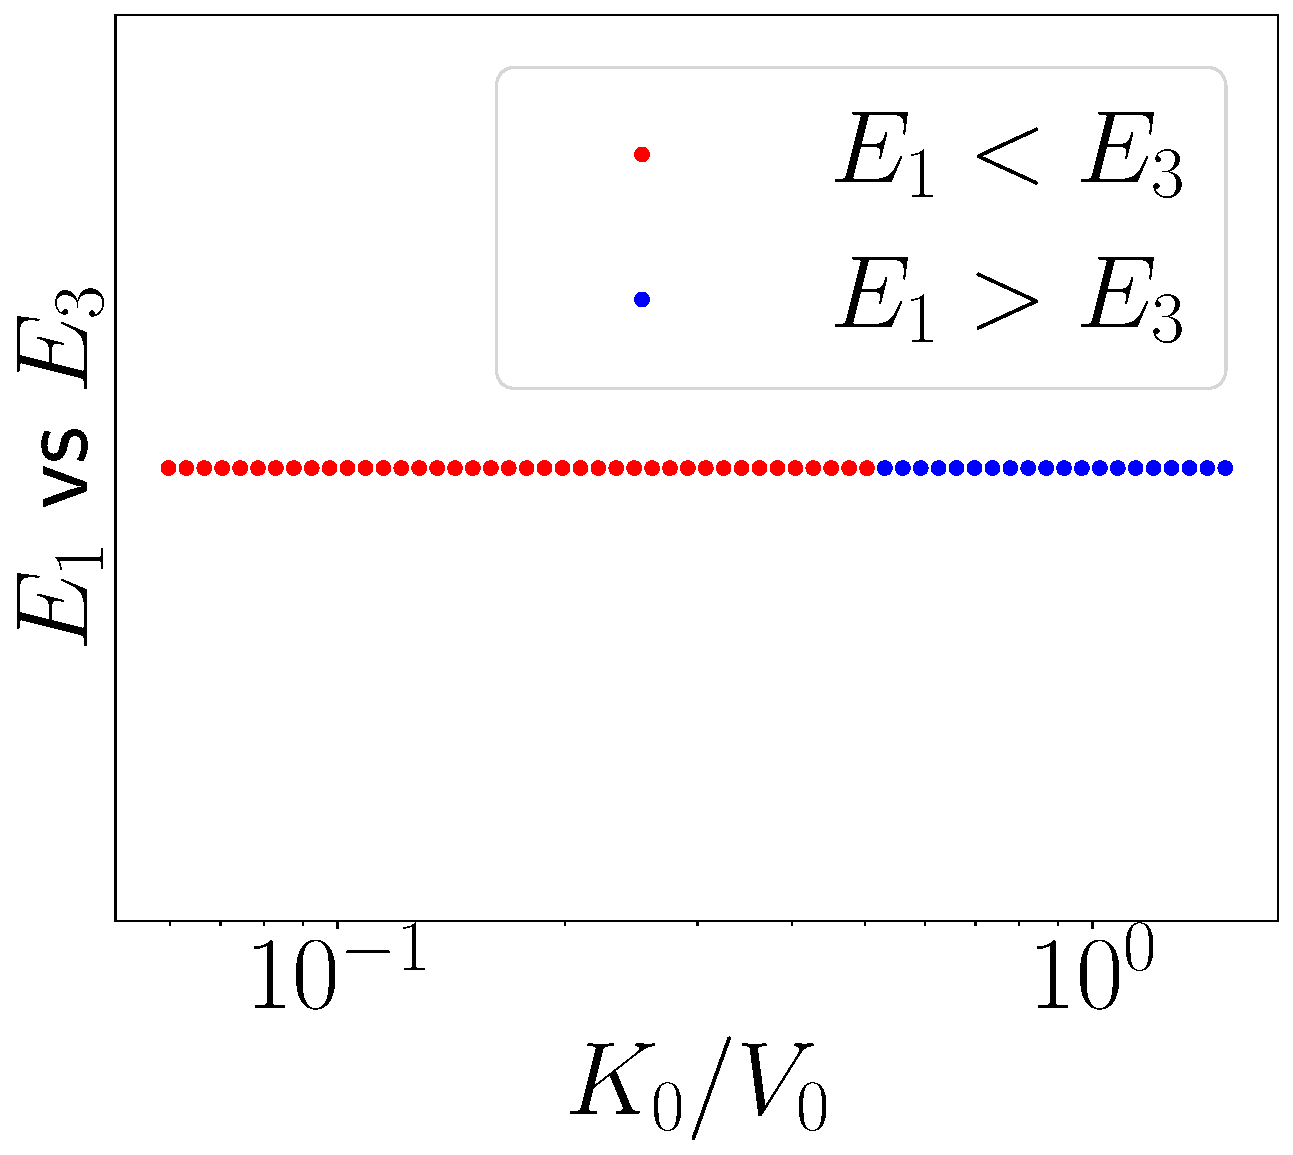
\includegraphics[width=0.5\textwidth]{../figures/E1_vs_E3.pdf}
\end{figure}

\section{Approach towards the thermodynamic limit}

{\bf \Large [Update with V vs D plots]}

The URG method works strictly on finite systems and leads to finite values of fixed point couplings. The behaviour of the Hamiltonian in the thermodynamic limit can then be determined using finite-size scaling where we increase the bandwidth and decrease the width of each RG step. When applied to the fixed point value of the impurity-bath hybridisation parameter \(V\) (fig.~\ref{V_vs_D}), it can be seen that the fixed point value increases as the system size is increased, implying that the continuum limit of \(V^*\) is \(\infty\). This holds for both \(V_0 > J_0\) and \(V_0 < J_0\), as shown in the two panels of fig.~\ref{V_vs_D}.
\begin{figure}[!htb]
	\centering
	\hspace*{\fill}
	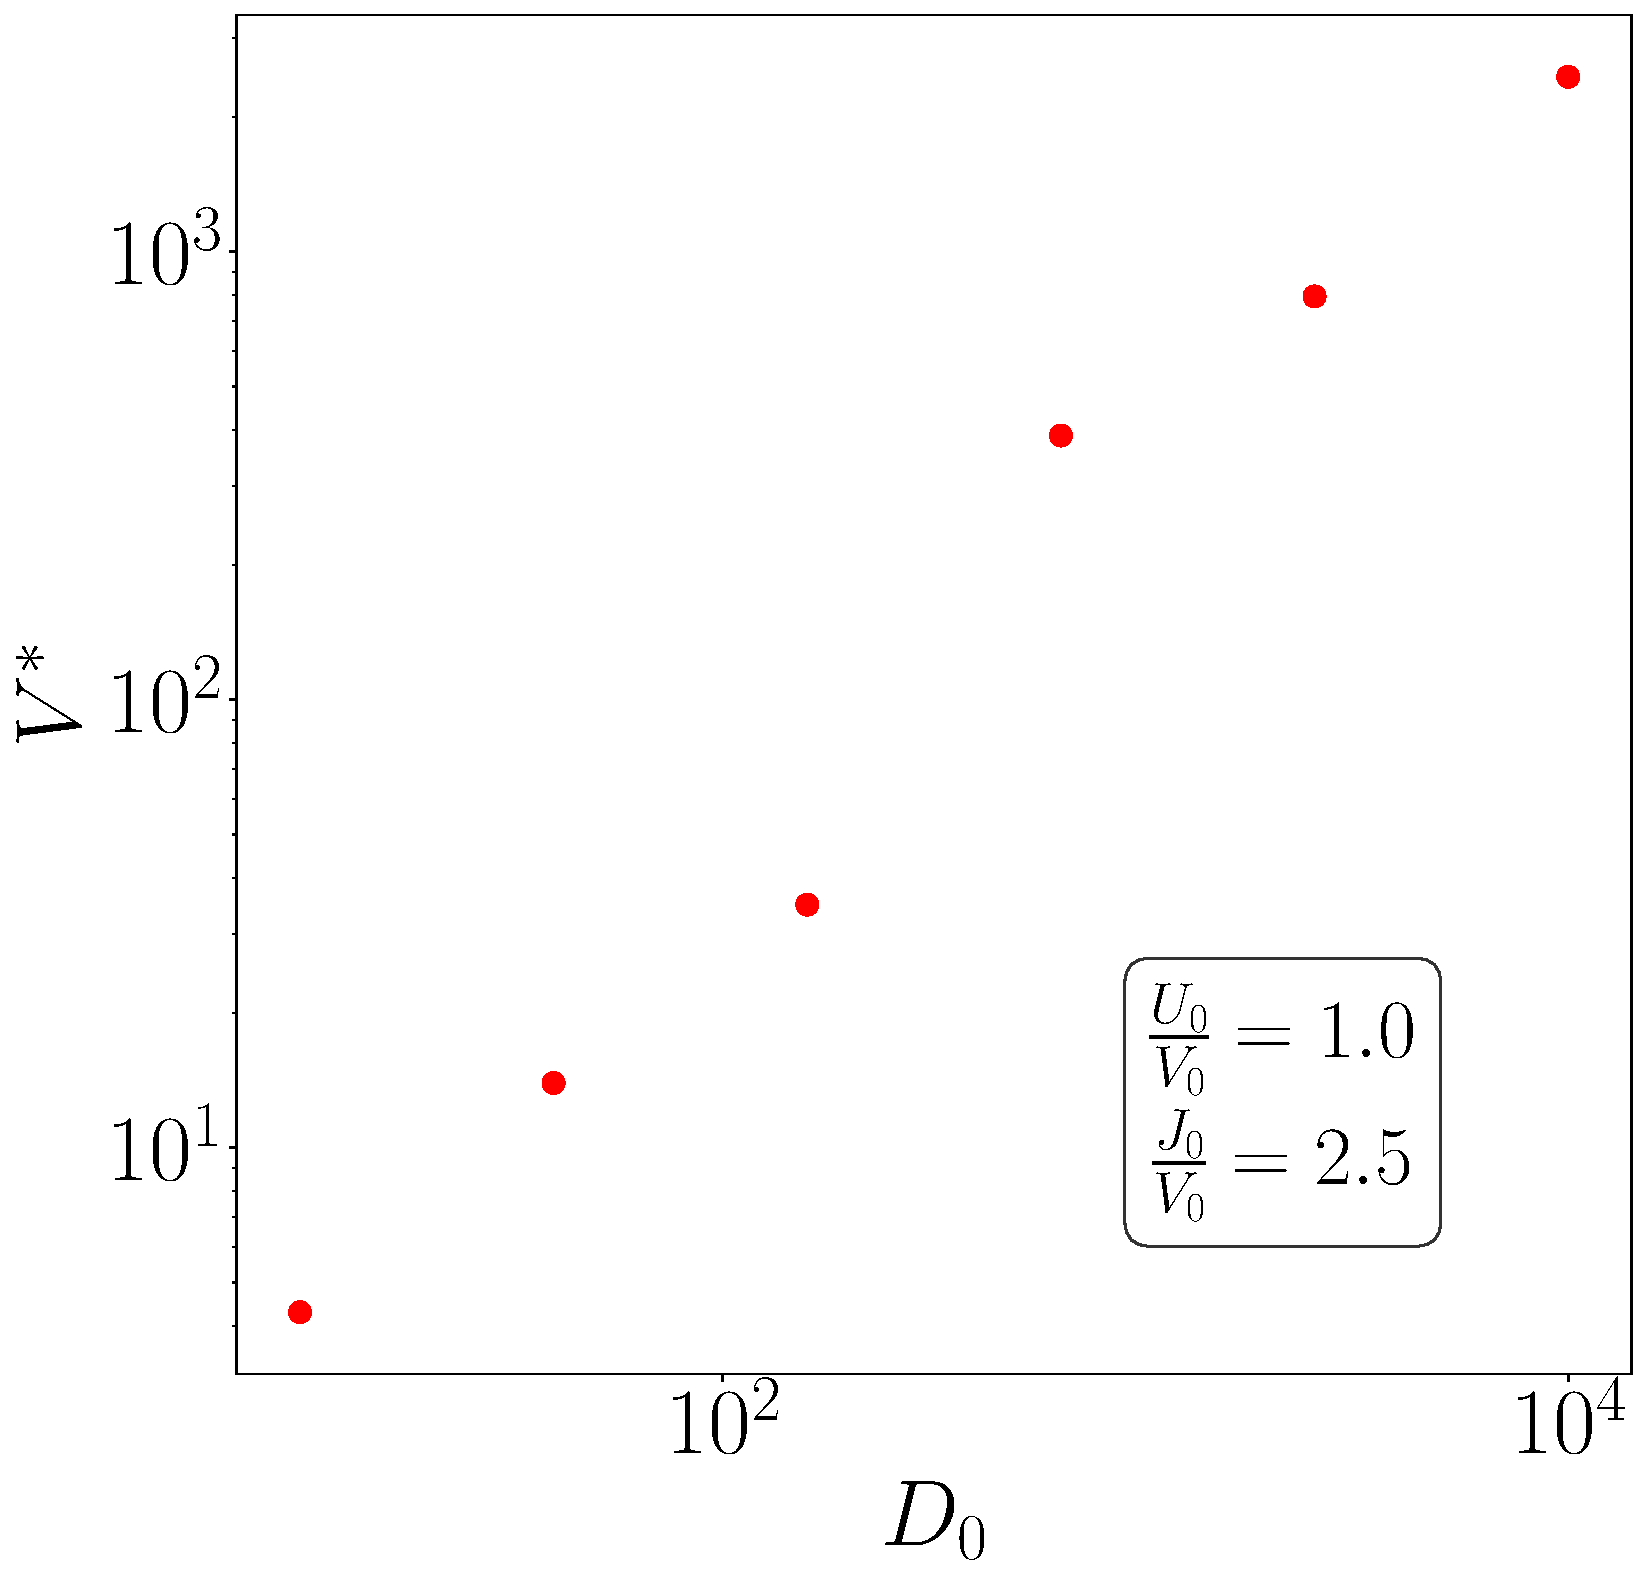
\includegraphics[width=0.4\textwidth]{../figures/Vstar_vs_D_smallV.pdf}
	\hspace*{\fill}
	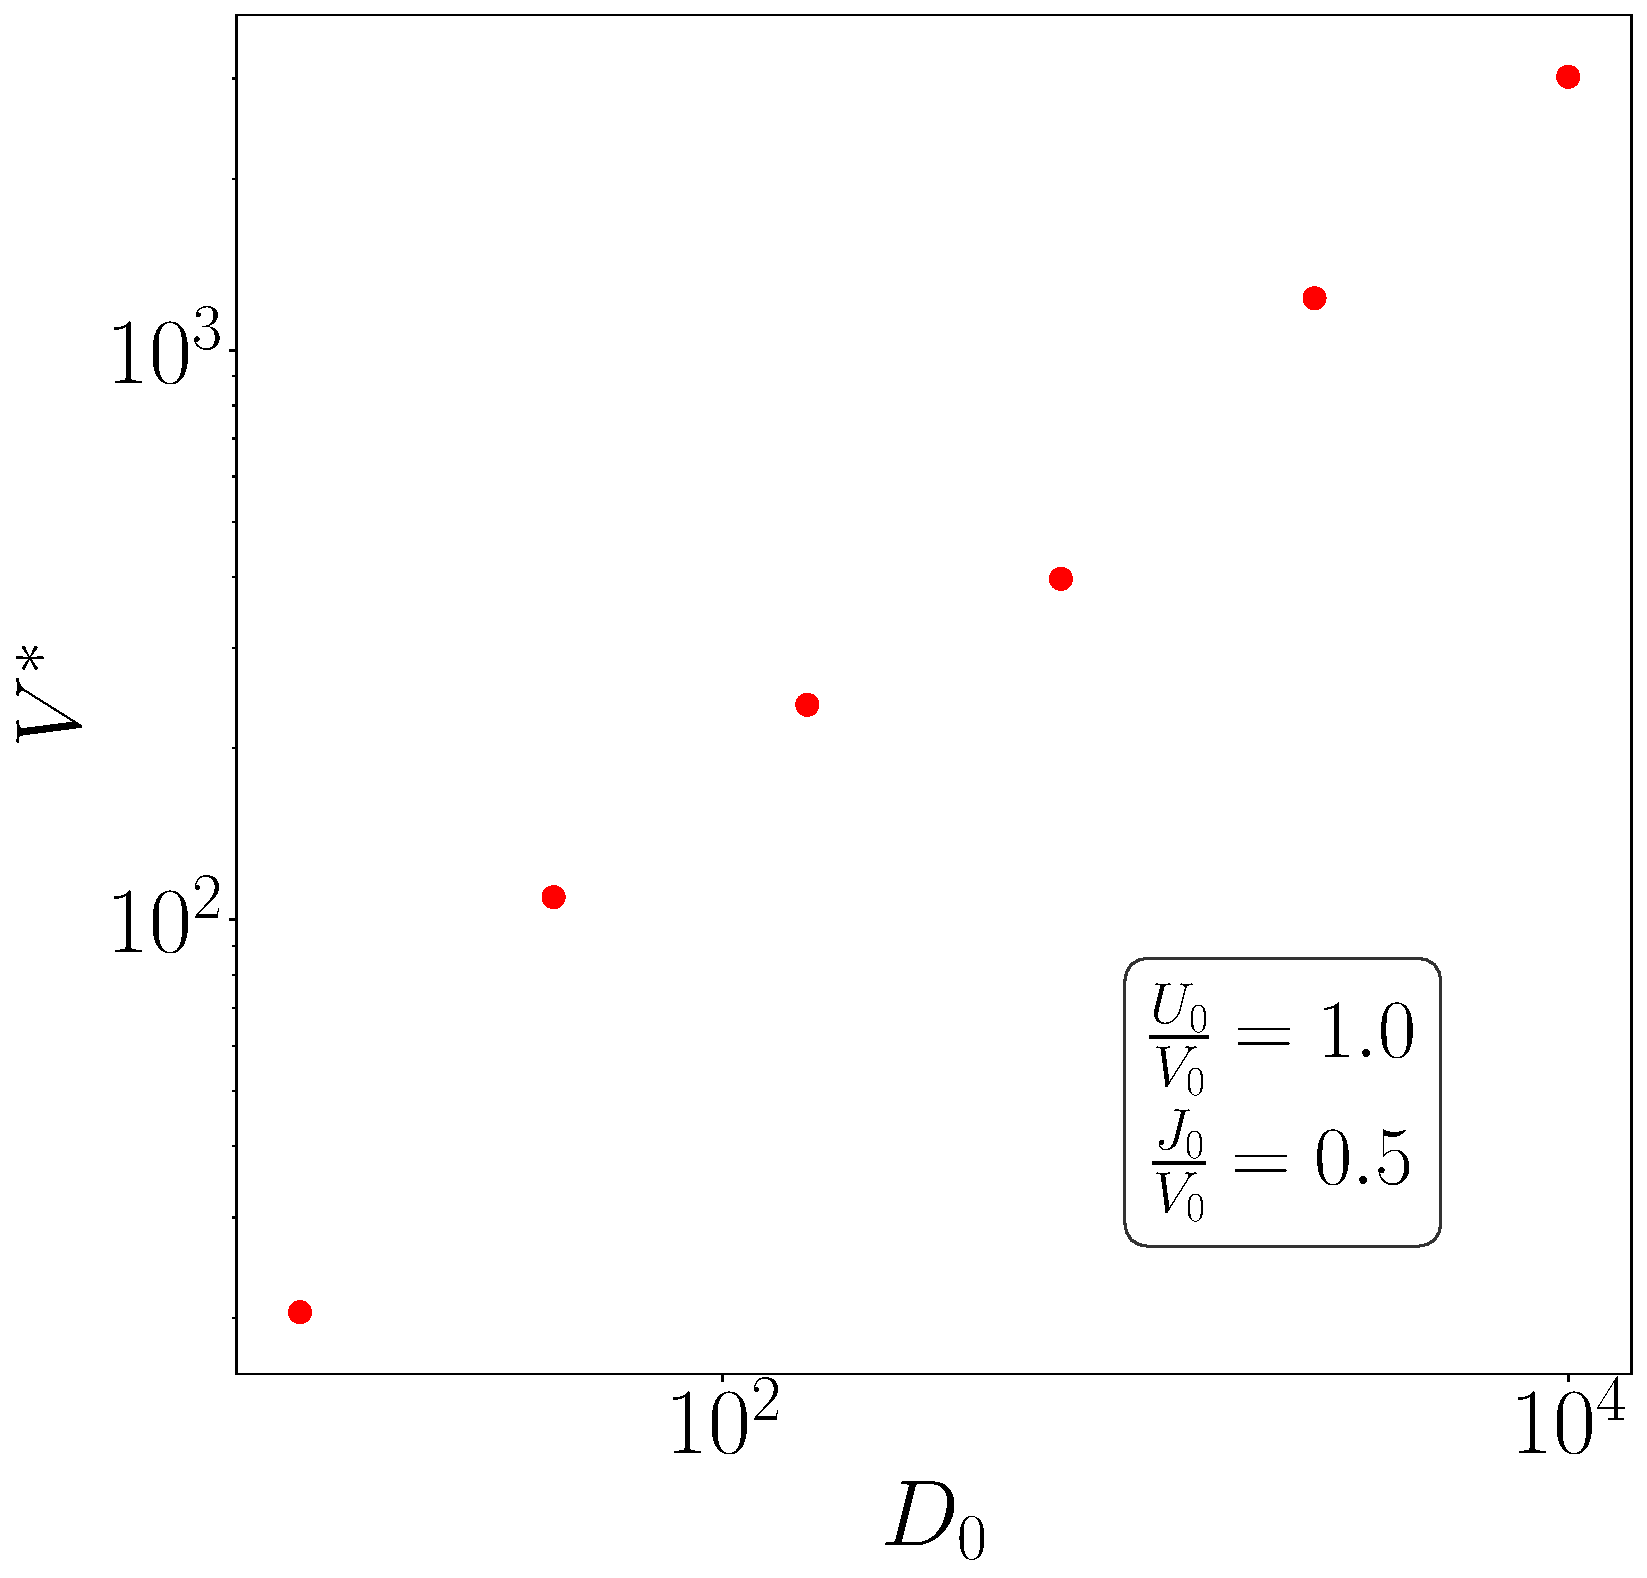
\includegraphics[width=0.4\textwidth]{../figures/Vstar_vs_D_largeV.pdf}
	\hspace*{\fill}
	\caption{Variation of fixed point value \(V^*\) with increasing bandwith \(D_0\), for both \(V_0 > J_0\) and \(V_0 < J_0\).}
	\label{V_vs_D}
\end{figure}

In a similar manner, we checked the variation of the spin and charge probabilities, \(c_s\) and \(c_c\), in the ground state, with increasing bandwith. The result is shown in fig.~\ref{c_vs_D}.
\begin{figure}[!htb]
	\centering
	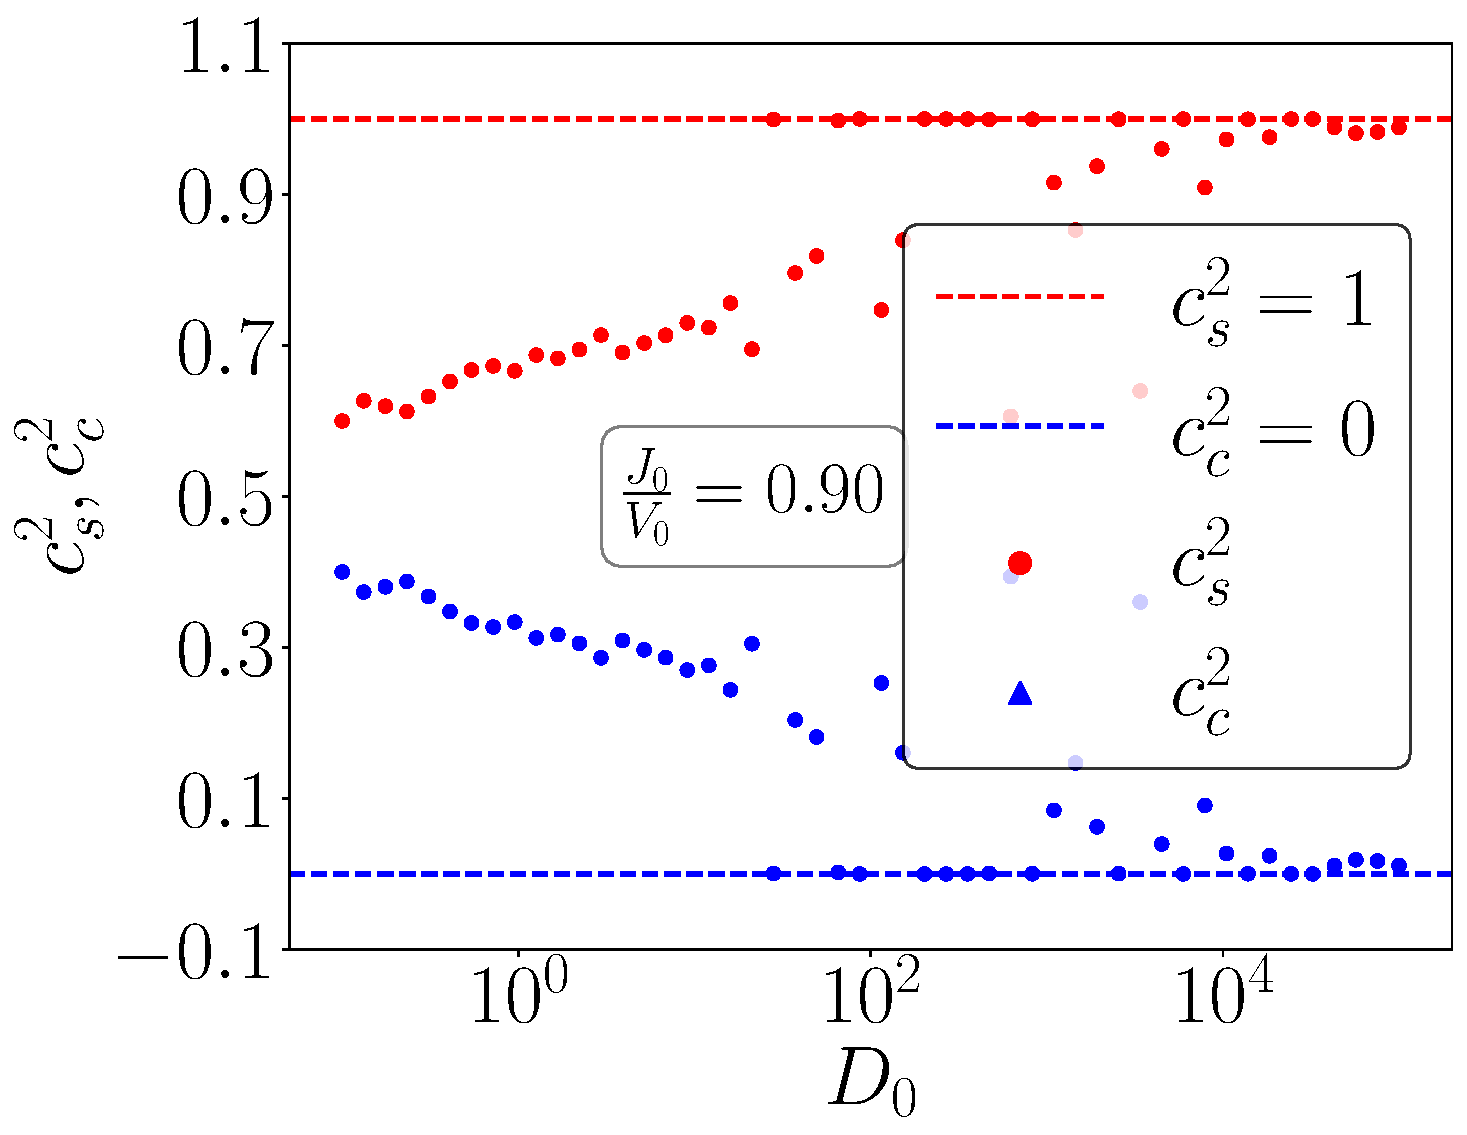
\includegraphics[width=0.45\textwidth]{../figures/coeffs_vs_D.pdf}
	\caption{Variation of spin and charge fractions, \(c_s\) and \(c_c\), of the ground state, as a function of bare bandwidth \(D_0\). Left and right panels show the cases of \(J_0 < V_0\) and \(J_0 > V_0\) respectively.}
	\label{c_vs_D}
\end{figure}
For both \(V_0 < J_0\) and \(V_0 > J_0\), we see that the spin contribution increases towards unity while the charge contribution vanishes. This indicates that at large bandwidth, the ground state becomes purely a spin singlet, formed purely by singly-occupied impurity states.
\begin{equation}\begin{aligned}
	\label{gstate_kondo}
	\lim_{D_0 \to \infty} \ket{\Psi}_1 = \frac{1}{\sqrt 2}\left(\ket{\uparrow, \downarrow} - \ket{\downarrow, \uparrow}\right) 
\end{aligned}\end{equation}

\section{Effective temperature scale at the fixed point}
We will first change the discrete RG equation to a continuum equation by interpreting \(\Delta J\) as \(\frac{\Delta J}{\Delta \ln D}\), where the denominator is unity: \(\Delta \ln D = 1\). Now, since the bandwidth is decreasing under the RG, we can write \(\Delta \ln D = -d \ln D\). The continuum equation (for \(K=0\)) becomes
\begin{equation}\begin{aligned}
	\frac{\:\mathrm{d}J}{\:\mathrm{d}\ln D} = n(0)J^2 \frac{1}{\omega - \frac{D}{2} + \frac{J}{4}}
\end{aligned}\end{equation}
where we have replaced by the number of states at each shell with that at the Fermi surface (uniform DOS). We can define a dimensionless quantity \(g \equiv \frac{J}{\frac{D}{2}} - \omega\). In terms of \(g\), the continuum RG equation becomes
\begin{equation}\begin{aligned}
	-\frac{\:\mathrm{d}g}{\:\mathrm{d}\ln D} + \frac{D g}{2\omega - D} = \frac{n(0) g^2}{1 - \frac{g}{4}}
\end{aligned}\end{equation}
Now, for the specific case where \(D\) is small (\(D \to 0\)), we can simplify and integrate this equation:
\begin{equation}\begin{aligned}
	\frac{\:\mathrm{d}g}{\:\mathrm{d}\ln D} &= \frac{n(0) g^2}{\frac{g}{4} - 1}\\
	\implies \left[\frac{1}{g} + \frac{1}{4}\ln g\right]_{g_0}^{g^*} &= n(0)\ln D\big\vert_{D_0}^{D^*}
\end{aligned}\end{equation}
\(g^*(_0), D^*(_0)\) are the fixed point (bare) values of \(g, D\). From the denominator structure, the fixed-point value is \(g^* =  4\). This gives an estimate of the bandwidth of the emergent window:
\begin{equation}\begin{aligned}
	D^* = D_0 \left( \frac{4}{g_0} \right)^\frac{1}{4n(0)}\exp\left\{-\frac{1}{n(0)}\left(\frac{1}{g_0} - \frac{1}{4}\right)\right\}
\end{aligned}\end{equation}
We can now define a temperature scale~\cite{wilson1975,hrk_wilson_1980} for the fixed-point theory:
\begin{equation}\begin{aligned}
	T_K \equiv \frac{2N^*}{\pi}D^* = \frac{2N^*}{\pi}D_0 \left( \frac{4}{g_0} \right)^\frac{1}{4n(0)}\exp\left\{-\frac{1}{n(0)}\left(\frac{1}{g_0} - \frac{1}{4}\right)\right\}
\end{aligned}\end{equation}
The factor of \(2N^*\) is inserted to make the Kondo temperature intensive (we will see below that the \(N^*\) allows it to  be written in terms of parameters of the two-site Hamiltonian) - \(2N^*\) is the total number of momentum states in the fixed point theory. The factor of \(\frac{1}{\pi}\) is for aesthetic reasons. Since we have and will primarily work with \(\omega=0\), the fixed point condition can be used to write \(D^* = \frac{J^* + K^*}{2}\).
\begin{equation}\begin{aligned}
	T_K = \frac{2N^*}{\pi}\frac{1}{2}\left(J^* + K^*\right) = \frac{1}{\pi}\left(j + k\right)
\end{aligned}\end{equation}
\section{Impurity susceptibilities}
\subsection{Spin susceptibility}
The spin susceptibility is defined as
\begin{equation}\begin{aligned}
	\label{chi_def}
	\chi(\beta) = \beta \left(\left<\left(S_d^z\right)^2\right> - \left<S_d^z\right>^2\right)
\end{aligned}\end{equation}
There is an alternate way of calculating this. We insert a fictitious magnetic field that couples only to the impurity site. The Hamiltonian in the presence of this field is
\begin{equation}\begin{aligned}
	\label{field_ham}
	\mathcal{H}^\prime(B) = \mathcal{H} + B S_d^z
\end{aligned}\end{equation}
The susceptibility is then given by
\begin{equation}\begin{aligned}
	\label{chi_exp}
	\chi(\beta) &= \lim_{B \to 0}\frac{1}{\beta}\left[\frac{1}{Z(B)} \frac{\partial^2{Z(B)}}{\partial{B^2}}-\frac{1}{Z(B)^2} \left(\frac{\partial{Z(B)}}{\partial{B}}\right)^2\right]
\end{aligned}\end{equation}
where \(Z(B)\) is the partition function of the Hamiltonian \(\mathcal{H}^\prime(B)\). The following is to prove that the RHS of eqs.~\ref{chi_def} and \ref{chi_exp} are the same. We start with \ref{chi_exp}. The first derivative can be written as
\begin{equation}\begin{aligned}
	\frac{\partial{Z(B)}}{\partial{B}} = \text{Trace}\left[\frac{\partial{}}{\partial{B}} \exp\left\{-\beta\left( \mathcal{H} + BS_d^z \right) \right\}\right] = \text{Trace}\left[-\beta S_d^z \exp\left\{-\beta\left( \mathcal{H} + BS_d^z \right) \right\}\right]
\end{aligned}\end{equation}
which means the first term becomes
\begin{equation}\begin{aligned}
	\lim_{B \to 0}-\frac{1}{Z(B)^2} \left(\frac{\partial{Z(B)}}{\partial{B}}\right)^2 = -\left(\beta \frac{1}{\text{Trace}\left[\exp\left\{-\beta\mathcal{H}\right\}\right]} \text{Trace}\left[S_d^z \exp\left\{-\beta\mathcal{H}\right\}\right]\right)^2 = -\beta^2 \left<S_d^z\right>^2
\end{aligned}\end{equation}
The second derivative is
\begin{equation}\begin{aligned}
	\frac{\partial^2{Z(B)}}{\partial{B^2}} = \text{Trace}\left[-\beta S_d^z  \frac{\partial{}}{\partial{B}}\exp\left\{-\beta \left( \mathcal{H} + BS_d^z \right) \right\}\right] = \text{Trace}\left[\beta^2 \left(S_d^z\right)^2 \exp\left\{-\beta \left( \mathcal{H} + BS_d^z \right) \right\}\right]
\end{aligned}\end{equation}
so the second term becomes
\begin{equation}\begin{aligned}
	\lim_{B \to 0}\frac{1}{Z(B)} \frac{\partial^2{Z(B)}}{\partial{B^2}} = \beta^2 \frac{1}{\text{Trace}\left[\exp\left\{-\beta \mathcal{H}\right\}\right]}\text{Trace}\left[\left(S_d^z\right)^2 \exp\left\{-\beta \mathcal{H}\right\}\right] = \beta^2 \left<\left(S_d^z\right)^2 \right>
\end{aligned}\end{equation}
The full thing becomes
\begin{equation}\begin{aligned}
	\lim_{B \to 0}\frac{1}{\beta}\left[\frac{1}{Z(B)} \frac{\partial^2{Z(B)}}{\partial{B^2}}-\frac{1}{Z(B)^2} \left(\frac{\partial{Z(B)}}{\partial{B}}\right)^2\right] = \frac{1}{\beta}\left(-\beta^2 \left<S_d^z\right>^2 + \beta^2 \left<\left(S_d^z\right)^2 \right>\right) \\
	= \beta \left(\left<\left(S_d^z\right)^2\right> - \left<S_d^z\right>^2\right) 
\end{aligned}\end{equation}
This completes the proof. 

To calculate the impurity susceptibility, we take the zero bandwidth Hamiltonian \(\mathcal{H}_{IR}\) and insert a magnetic field to obtain the Hamiltonian in eq.~\eqref{field_ham}. For a particular regime of \(U\), only one of \(J\) or \(K\) will be non-zero. We then numerically diagonalise this Hamiltonian to obtain the partition function \(Z(B)\) and its derivatives. The spin susceptibility can then be calculated using eq.~\eqref{chi_exp}. The results for \(U>0\) are shown in fig.~\ref{chi}.
\begin{figure}[!htb]
	\centering
	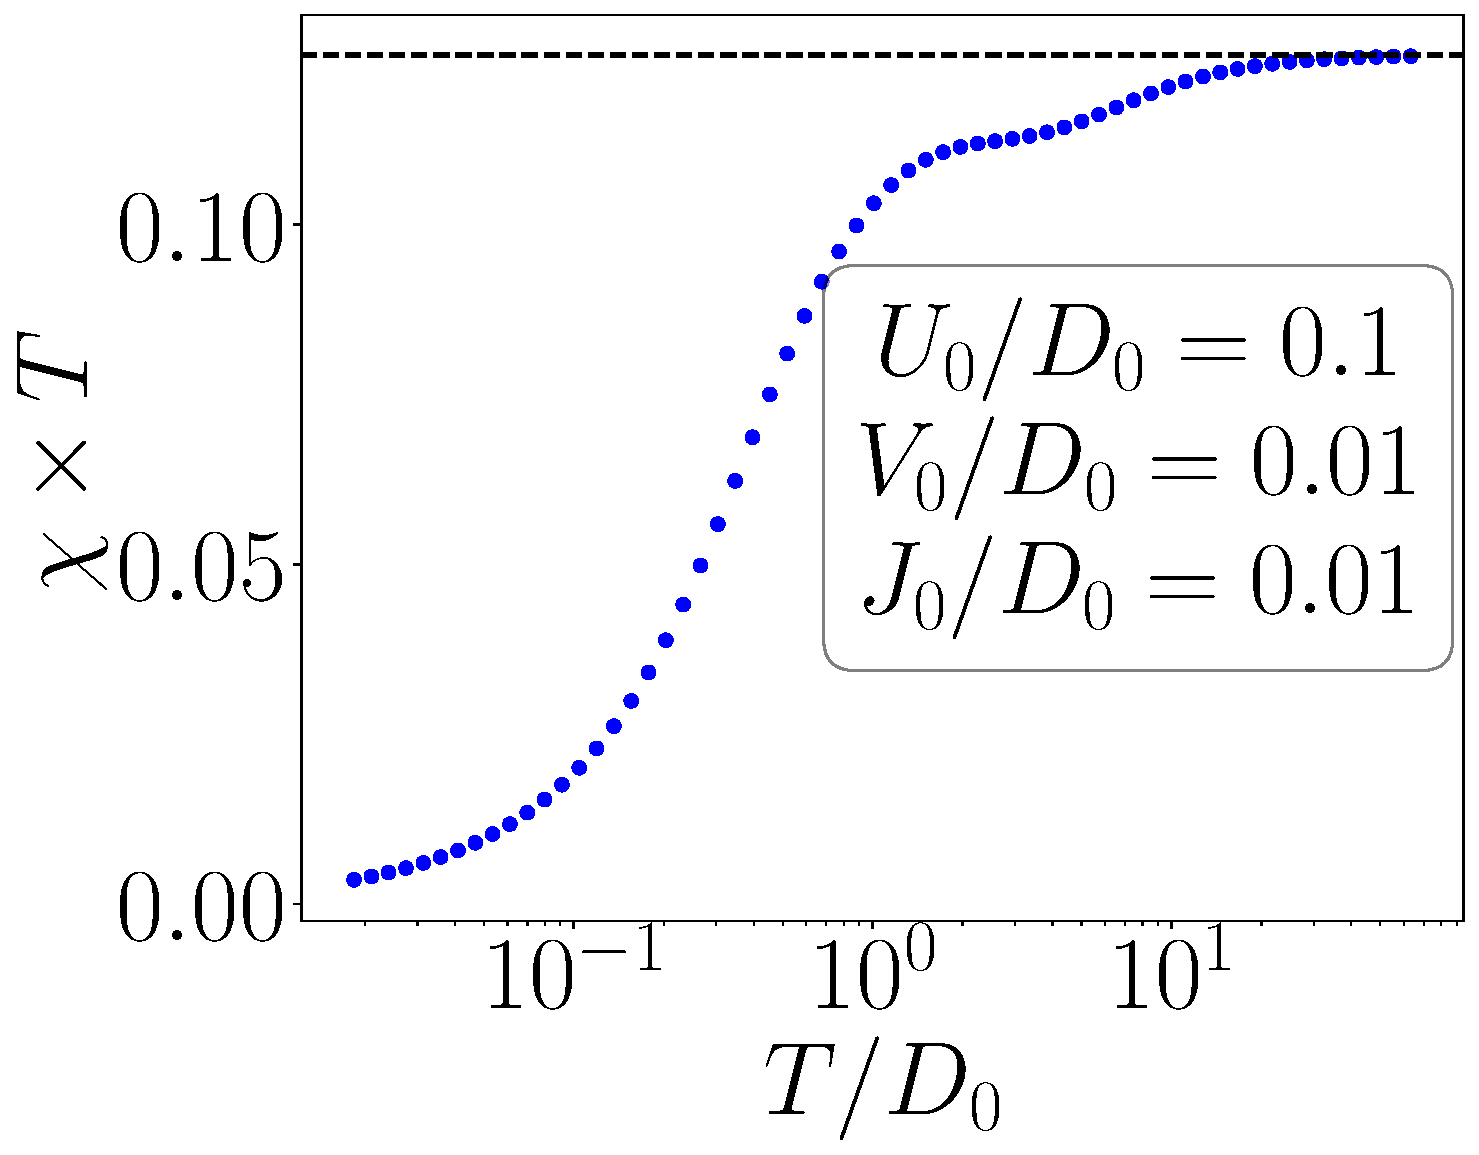
\includegraphics[width=0.49\textwidth]{../figures/chiT.pdf}
	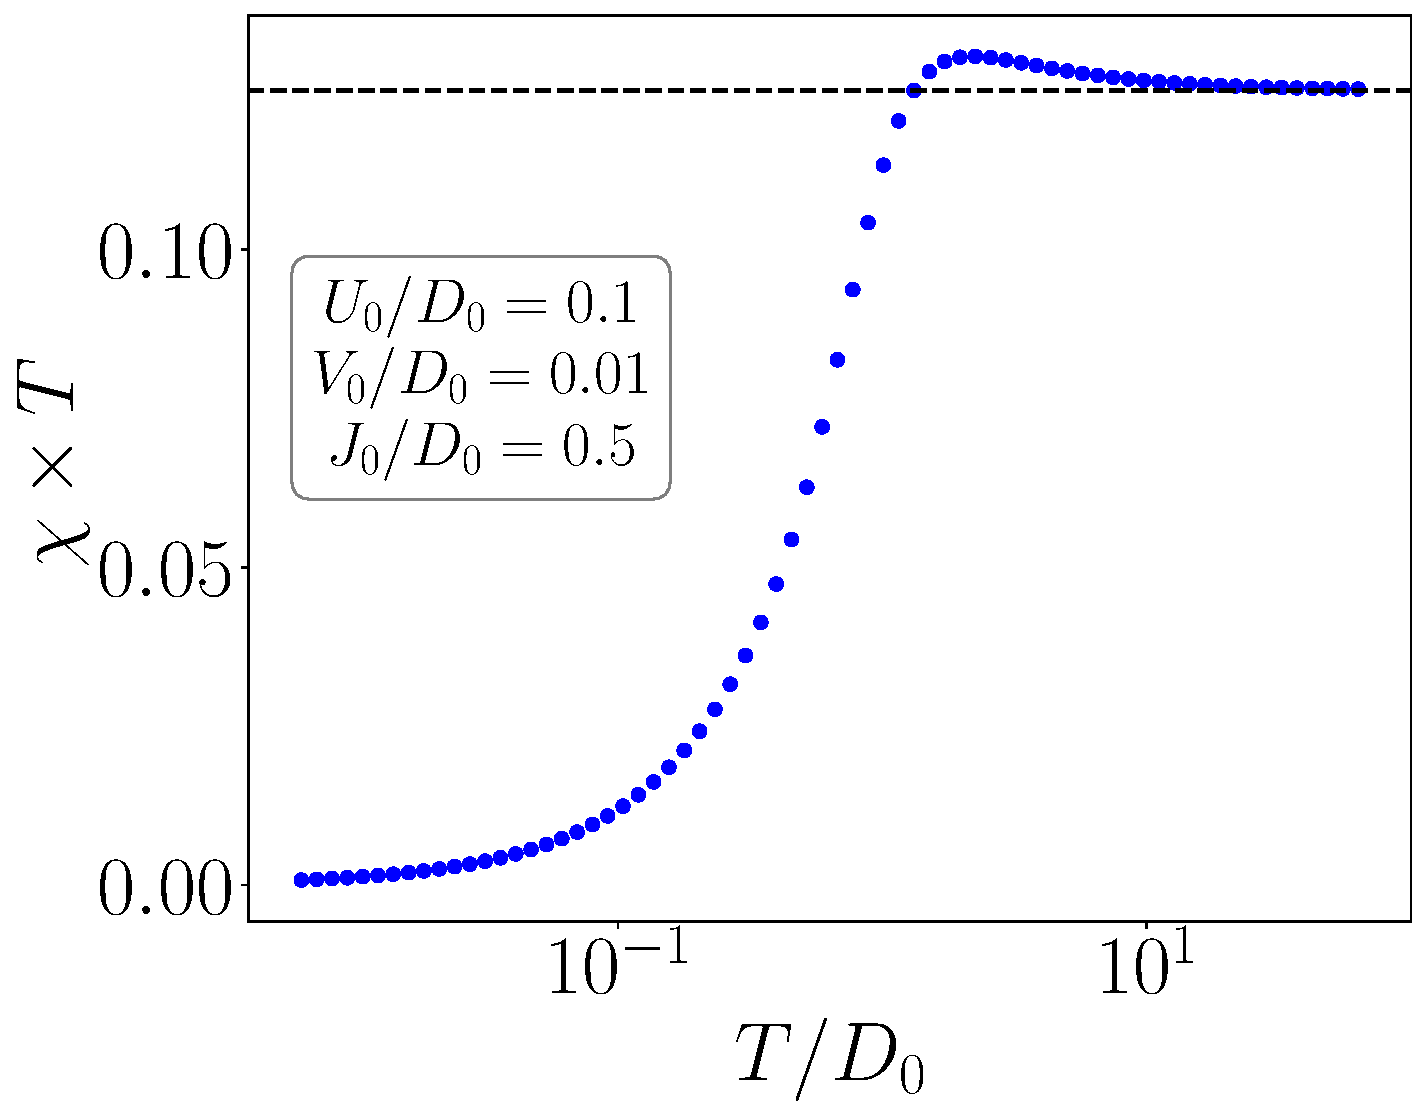
\includegraphics[width=0.49\textwidth]{../figures/chiT_large.pdf}
	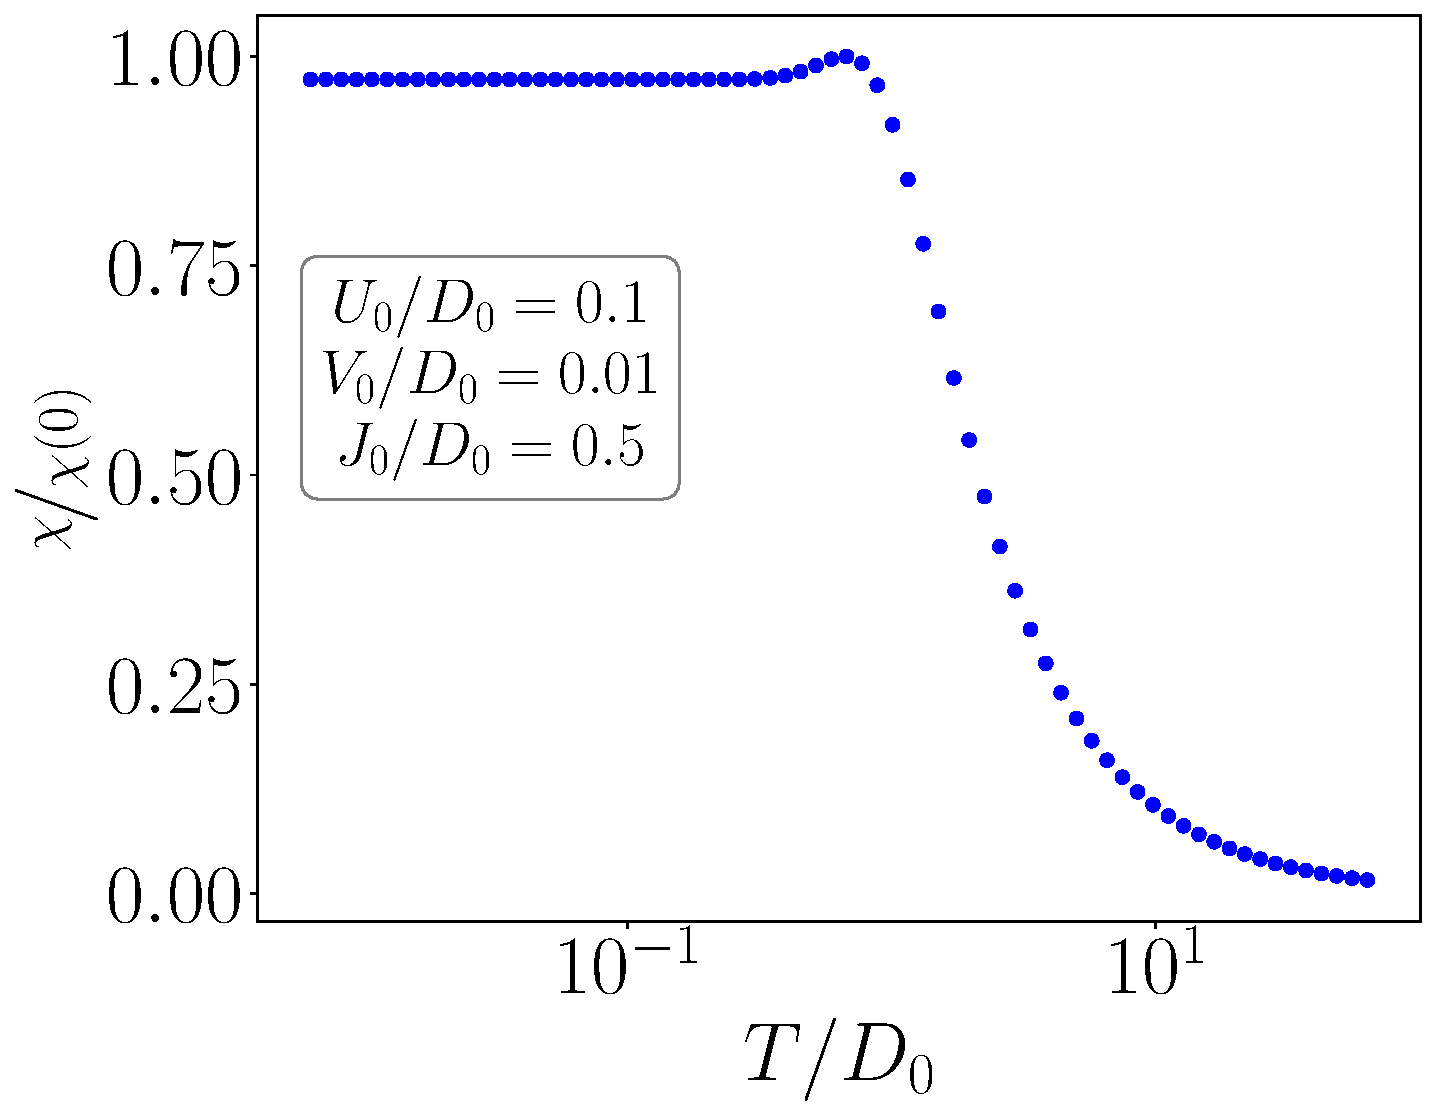
\includegraphics[width=0.49\textwidth]{../figures/chi.pdf}
	\caption{Spin susceptibility of the impurity times temperature, for two sets of bare parameters, in \(U>0\). At low temperatures, it becomes linear because \(\chi\) itself becomes constant (screening), while at high temperatures, \(\chi\times T\) becomes constant because of the paramagnetic \(\sim 1/T\) form of \(\chi\). For the right panel with a larger value of the spin-exchange coupling, the \(\chi\) tries to go towards the local moment value of \(1/4\) but eventually drops back to the free orbital value of \(1/8\).}
	\label{chi}
\end{figure}

\subsection{Charge susceptibility}
We can similarly define the charge susceptibility as
\begin{equation}\begin{aligned}
	\label{zero_chi_charge}
	\chi(\beta) = \beta \left(\left<\left(C_d^z\right)^2\right> - \left<C_d^z\right>^2\right) = \lim_{B_c \to 0}\frac{1}{\beta}\left[\frac{1}{Z(B_c)} \frac{\partial^2{Z(B_c)}}{\partial{B_c^2}}-\frac{1}{Z(B_c)^2} \left(\frac{\partial{Z(B_c)}}{\partial{B_c}}\right)^2\right]
\end{aligned}\end{equation}
where \(B_c\) is now a field that couples to the impurity charge-isospin:
\begin{equation}\begin{aligned}
	\label{charge_field}
	\mathcal{H}^\prime(B_c) = \mathcal{H} + B_c C_d^z
\end{aligned}\end{equation}
The charge susceptibility for \(U<0\) is shown in fig.~\ref{chi_charge}.
\begin{figure}[!htb]
	\centering
	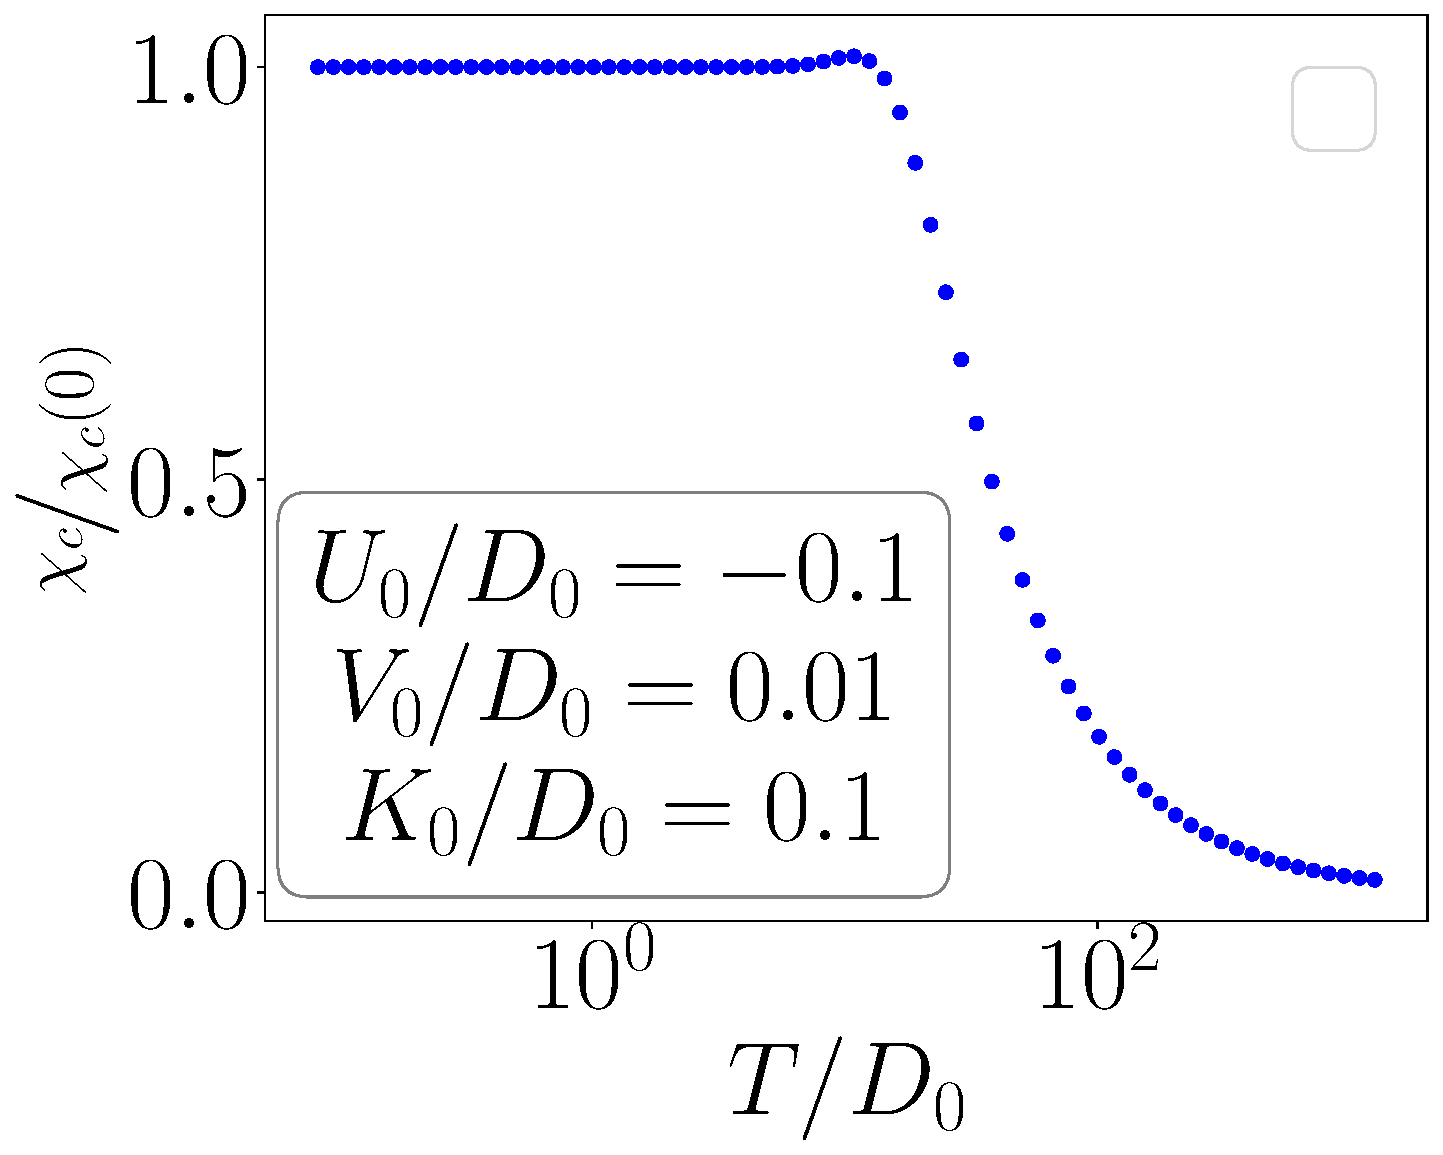
\includegraphics[width=0.49\textwidth]{../figures/chic.pdf}
	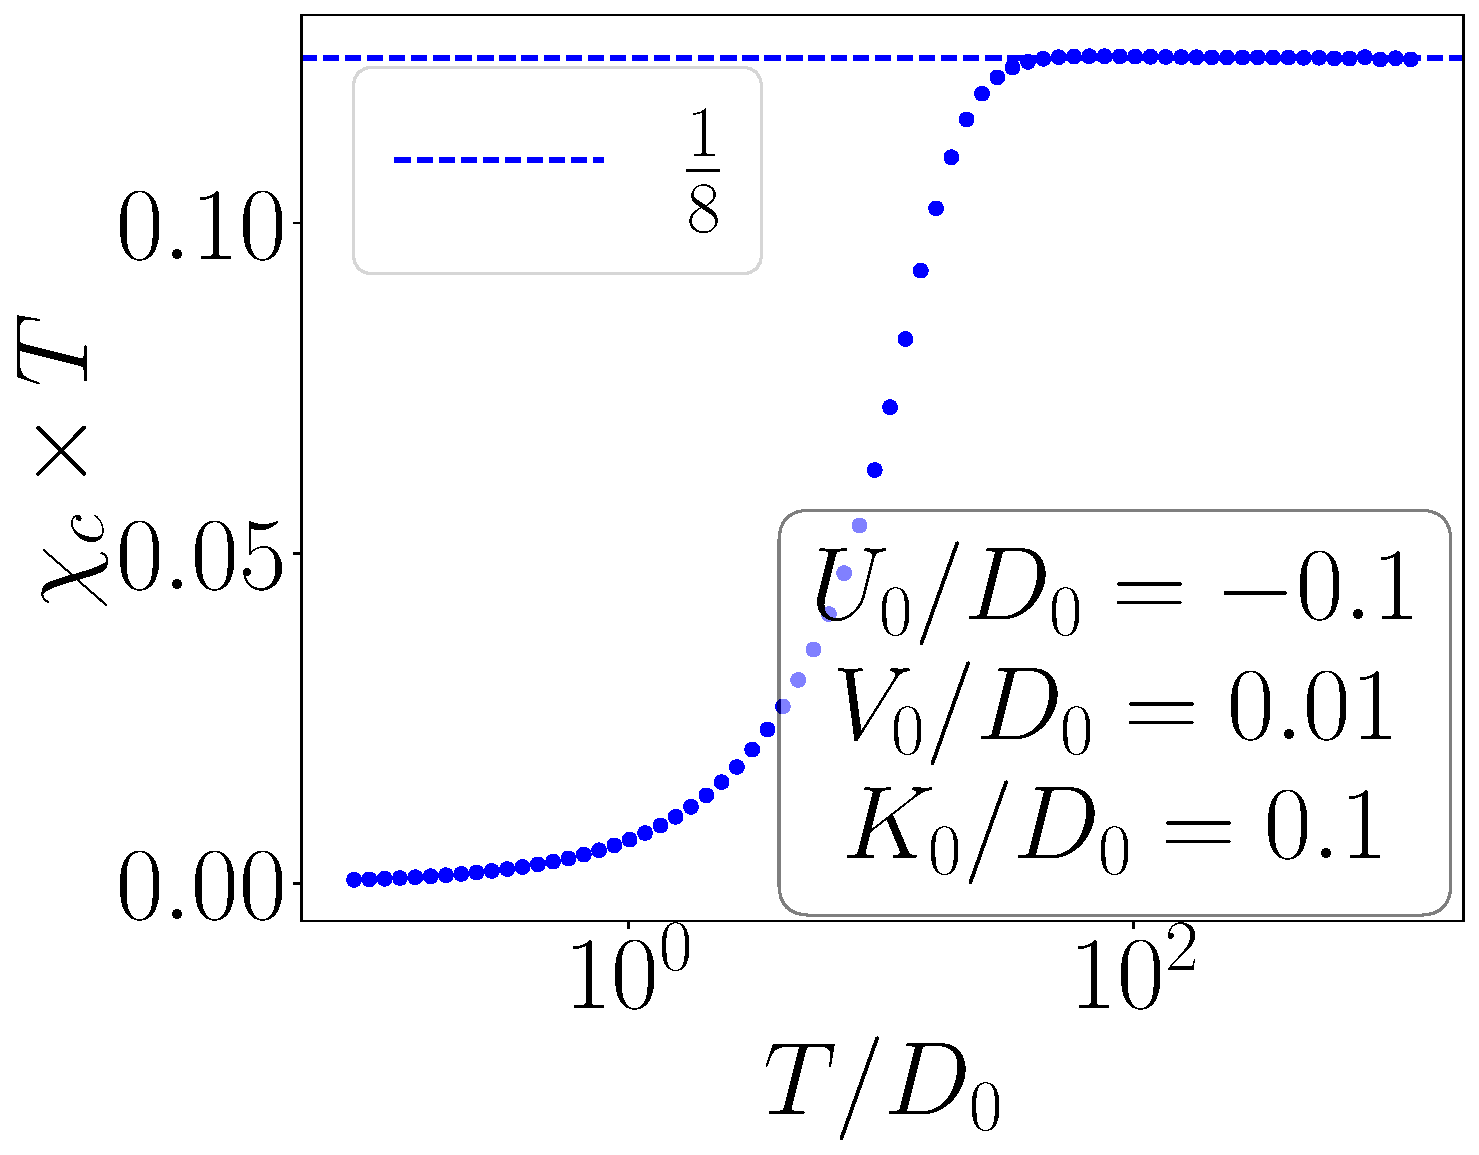
\includegraphics[width=0.49\textwidth]{../figures/chic_T.pdf}
	\caption{Charge susceptibility for the impurity at \(U<0\), for two sets of bare parameters. The physics is very similar to that of the spin susceptibility in \(U>0\).}
	\label{chi_charge}
\end{figure}

It is interesting to look at the behaviour of the charge susceptibility in the positive \(U\) regime, fig.~\ref{chi_charge_posU}. It  is seen that for \(J_0<V_0\), the charge susceptibility is very similar to the spin susceptibility, with a reduced saturation value. This is because, for that range of bare values, the ground state consists of a comparable mixture of the spin and charge states (see fig.~\ref{cs_cc}). This means that the magnetic field term in eq.~\eqref{charge_field} can couple to the charge component of the ground state, and give a non-zero charge susceptibility at zero temperature. On the other hand, for \(J_0 > V_0\), we see that \(\chi_c\) vanishes at low temperatures. This can again be understood from the ground state. For that range of bare values, the ground state can be approximated by purely the singlet, because the charge fraction \(c_-^c\) becomes very small. This means that the field \(B_c \) has nothing to couple with. Alternatively, it can be said that since the ground state has only terms with \(\hat n_d=1\), no number fluctuation is possible, and the impurity isospin is not susceptible at all to charge polarisation.
\begin{figure}[!htb]
	\centering
	\includegraphics[width=0.48\textwidth]{../figures/chiC_posU_J0=10.pdf}
	\includegraphics[width=0.48\textwidth]{../figures/chiC_posU_J0=40.pdf}
	\caption{Charge susceptibility of the impurity in the positive \(U\) regime, for two values of \(J_0\). The smaller bare value leads to a spin+charge mixed ground state, and hence a non-zero \(\chi_c\) at zero temperature. The larger \(J_0\), however, leads to a purely spin ground state without any number fluctuation, and this gives vanishing \(\chi_c\) at zero temperature.}
	\label{chi_charge_posU}
\end{figure}

From eq.~\eqref{gstate_kondo}, we know that in the thermodynamic limit, the ground state of \(U>0\) regime reduces to a screened local moment. That then implies that the charge susceptibility vanishes at low temperatures, owing to lack of any charge content in the ground state in the large bandwidth limit.
\begin{equation}\begin{aligned}
	\lim_{D_0 \to \infty}\chi_c(U>0, T \to 0) = 0
\end{aligned}\end{equation}

\section{Specific heat}
The specific heat is calculated by diagonalizing the fixed point Hamiltonian, numerically. The obtained spectrum is denoted by \(\left\{ \mathcal{E}_i \right\} \). The total average energy of the impurity+cloud at temperature \(T\) is then
\begin{equation}\begin{aligned}
	\left<\mathcal{E} \right> = \frac{1}{Z}\sum_{i} \mathcal{E}_i e^{-\beta \mathcal{E}_i}
\end{aligned}\end{equation}
where \(Z = \sum_{i} e^{-\beta E_i}\) is the partition function. The specific heat of this system is thus
\begin{equation}\begin{aligned}
	C_V &= \frac{\partial{\left<\mathcal{E} \right>}}{\partial{T}} \\
	    &= -\frac{1}{k_B T^2} \frac{\partial{\left<\mathcal{E} \right>}}{\partial{\beta}} \\
	    &= \frac{1}{k_B T^2}\left[\frac{1}{Z}\sum_i \mathcal{E}_i^2 e^{-\beta \mathcal{E}_i} - \left(\frac{1}{Z}\sum_i \mathcal{E}_i e^{-\beta \mathcal{E}_i}\right)^2 \right] 
\end{aligned}\end{equation}
In the absence of impurity, the eigenvalues of the Hamiltonian are \(\left\{\mathcal{E}_i^0\right\}\) with a partition function \(Z^0 = \sum_{i} e^{-\beta E_i^0}\), so the bath specific heat is
\begin{equation}\begin{aligned}
	C_V^0 &= \frac{1}{k_B T^2}\left[\frac{1}{Z_0}\sum_i \mathcal{E}_i^2 e^{-\beta \mathcal{E}_i^0} - \left(\frac{1}{Z_0}\sum_i \mathcal{E}_i^0 e^{-\beta \mathcal{E}_i^0}\right)^2 \right] 
\end{aligned}\end{equation}
The impurity specific heat is the difference.
\begin{equation}\begin{aligned}
	C_V^\text{imp} = C_V - C_V^0
\end{aligned}\end{equation}
These values were calculated numerically and plotted against temperature in fig.~\ref{cv}.
\begin{figure}[!htb]
	\centering
	\includegraphics[width=0.6\textwidth]{../figures/Cv.pdf}
	\caption{Impurity specific heat}
	\label{cv}
\end{figure}

\section{Renormalization of impurity spectral function}
In this section we will obtain the impurity spectral function~\cite{costi2000,rosch_costi2003,bullaNRGreview}, which is defined in terms of the impurity Green's function as
\begin{equation}\begin{aligned}
	\mathcal{A(\omega)} = -\frac{1}{\pi}\text{ Im }\left[G_{dd}^\sigma\left( \omega \right) \right] 
\end{aligned}\end{equation}
The zero temperature retarded Green's function for the impurity, in the frequency domain, can be written as (see Appendix.~\ref{appx-spectral-func})
\begin{equation}\begin{aligned}
	\mathcal{A(\omega)} = \frac{1}{d_0}\sum_{n,0}\left[||\bra{0}\mathcal{O}_{\sigma}\ket{n}||^2\delta\left(\omega + E_0 - E_n\right) + ||\bra{n}\mathcal{O}_{\sigma}\ket{0}||^2\delta\left(\omega - E_0 + E_n\right)\right]
\end{aligned}\end{equation}
where \(\mathcal{O}_\sigma = c_{d\sigma} + S_d^- c_{0\overline\sigma} + S_d^z c_{0\sigma}\) is the excitation whose spectral function we are interested in. The excitations defined in \(\mathcal{O}\) incorporates both single-particle excitations brought about by the hybridisation as well as two-particle spin excitations brought about by the spin-exchange term
Since this is in terms of the exact eigenstates, it is a discrete sum of delta-functions. In practice, we get a continuous distribution. To compare with experiment, we need to convert the discrete sum into a continuous function. Following \cite{bullaNRGreview}, we replace the delta-functions at \(\pm x_n \equiv \pm(E_n - E_0)\) by normalized Gaussian functions
\begin{equation}\begin{aligned}
	\delta(\omega \pm x_n) \to \frac{1}{\eta_n\sqrt \pi}e^{-\left(\frac{\omega \pm x_n}{\eta_n}\right)^2}
\end{aligned}\end{equation}
The parameter \(\eta_n\) determines the height and width of the Gaussian, and is chosen such that the higher energy poles are broader than the lower energy ones:
\begin{equation}\begin{aligned}
	\eta_n = 4\Delta + \frac{1}{2}|x_n| 
\end{aligned}\end{equation}
\(\Delta = \pi \rho(0)V^2\) is the relevant energy scale for the non-interacting \((U=0)\) problem, \(\rho(0)\) being the density of states of the conduction bath at the Fermi energy. As a result, the function that we will numerically compute and plot is
\begin{equation}\begin{aligned}
	\mathcal{A(\omega)} &= \sum_{n,0}\frac{1}{d_0 \sqrt \pi \eta_n}\left[||\bra{0}c_{d\sigma}\ket{n}||^2e^{-\left(\frac{\omega - x_n}{\eta_n}\right)^2} + ||\bra{n}c_{d\sigma}\ket{0}||^2e^{-\left(\frac{\omega + x_n}{\eta_n}\right)^2}\right]
\end{aligned}\end{equation}
From the results of Langreth \cite{langreth1966}, we know that the spectral function at zero frequency is fixed by the occupancy of the impurity. Since we are in the particle-hole symmetric regime, this occupancy is fixed at 1, and hence so is the spectral function height at \(\omega = 0\). This result has been used to fix the spectral function height at the center during the computations. The fixed-point Hamiltonian \(H^*\) is diagonalized numerically to obtain \(\left\{E_n, \ket{n}\right\}\), for various values of the couplings. The intention here is to get an idea of how the spectral function morphs under the RG. Doing an actual reverse RG (described in \ref{rev_rg}) would require us to diagonalize a huge Hamiltonian. We take the simpler route of tuning the \(U\) from zero to soem large value. This should mimic the journey from the IR theory \((U=0)\) to the UV theory \((U \gg 0)\).

The spectral function is plotted for three sets of values in fig.~\ref{spec_func}. For low values of \(U\), the profile is that of a single peak at zero frequency. This is expected because at the low energy effective theory, the high energy Hubbard side bands have been integrated out. As \(U\) increases, shoulder-like structures appear on either side of the peak, which finally, at larger \(U\), develop into two side-peaks. This is the microscopic theory, where high energy features are also relevant.
\begin{figure}[!htb]
	\centering
	\includegraphics[width=0.4\textwidth]{../figures/spec_func_Ub=0_U_by_delta=0.00.pdf}
	\includegraphics[width=0.4\textwidth]{../figures/spec_func_Ub=0_U_by_delta=3.00.pdf}
	\includegraphics[width=0.4\textwidth]{../figures/spec_func_Ub=0_U_by_delta=5.00.pdf}
	\includegraphics[width=0.4\textwidth]{../figures/spec_func_Ub=0_U_by_delta=10.00.pdf}
	\includegraphics[width=0.4\textwidth]{../figures/spec_func_Ub=0_U_by_delta=25.00.pdf}
	\caption{Impurity spectral function for multiple values of \(U\). The increase in value of \(U\) is accompanied by the appearance of the side-peaks.}
	\label{spec_func}
\end{figure}
The physics of the three peaks can now be looked into. Since the central peak is at zero energy, it has to do with excitations that do not cost any energy. There are two such excitations: excitations within the spin sector and within the charge sector.
\begin{equation}\begin{aligned}
	\ket{\uparrow} \mathrel{\mathlarger{\mathlarger{\mathop{\rightleftarrows}}^{J S_d^-}_{JS_d^+}}}\ket{\downarrow}, &&&&\ket{\Uparrow} \mathrel{\mathlarger{\mathlarger{\mathop{\rightleftarrows}}^{K C_d^-}_{K C_d^+}}}\ket{\Downarrow}\\
\end{aligned}\end{equation}
The thick arrow \(\Uparrow\) represents the charge isospin. At particle-hole symmetry, both the spin configurations has energy of \(\epsilon_d\), while the charge configurations have energy of \(2\epsilon_d + U=0\) and 0. Hence, no energy is required for these excitations, which is why see a macroscopic number of cloud electrons resonating with the impurity at the Fermi surface. Also note that if \(\hat S_i\) and \(\hat C_j\) are two operators of the spin and charge sector (\(i,j \in \left\{ x,y,z \right\} \)), then
\begin{equation}\begin{aligned}
	\hat S_i \hat C_j = \hat C_j \hat S_i = 0
\end{aligned}\end{equation}
We can see this by applying that operator on a basis state. Since the set of four states 
\begin{equation}\begin{aligned}
	\ket{\hat S_i = \pm \frac{1}{2}, \hat C_j = 0}, \ket{\hat S_i = 0, \hat C_j = \pm\frac{1}{2}}
\end{aligned}\end{equation}
are all independent, they form a basis. If we apply the operator on these states:
\begin{equation}\begin{aligned}
	\hat S_i \hat C_j \ket{\hat S_i} &= 0, &&&&\hat C_j \hat S_i \ket{S_i} = S_i \hat C_j \ket{S_i} = 0\\
	\hat C_j \hat S_i \ket{C_j} &= 0, &&&&\hat S_i \hat C_j \ket{\hat C_j} = C_j \hat S_i \ket{\hat C_j} = 0 \\
\end{aligned}\end{equation}
This shows that each operator acts only on its own subspace. \(S_i\) does not act on the charge sector, and vice-versa. There is no single-particle excitation here.

The physics of the side-peaks is that of single number fluctuations on the impurity. These are brought about by the term \(Vc^\dagger_{0\sigma}c_{d\sigma} + \text{h.c.}\).
\begin{equation}\begin{aligned}
	\left( \epsilon_d  \right) \ket{\sigma} & \mathrel{\mathlarger{\mathlarger{\mathop{\rightleftarrows}}^{V c^\dagger_{d\overline\sigma}/V c_{d\sigma}}_{V c_{d\overline\sigma}/V c^\dagger_{d\sigma}}}} &\ket{n_d=2,0} \left( 0 \right) \\
\end{aligned}\end{equation}
These transitions involve energy transfer of the order of \(\epsilon_d\). This is why, at very small \(U\), they remain absorbed inside the central peak. These transitions do not involve any spin or charge-flip, rather they take the impurity between the spin and charge sectors.

\section{Effective Hamiltonian for excitations of the Kondo cloud}
To find an effective Hamiltonian for the excitations of the Kondo cloud, we will integrate out the impurity part of the wavefunction. The Schrodinger equation for the \(J > K\) ground state is
\begin{equation}\begin{aligned}
	E_g &\left[c_-^s \left(\ket{\uparrow, \downarrow} - \ket{\downarrow, \uparrow}\right) + c^c_- \left(\ket{\uparrow\downarrow, 0} + \ket{0, \uparrow\downarrow}\right)\right] \\
	    &= \mathcal{H} \left[c_-^s \left(\ket{\uparrow, \downarrow} - \ket{\downarrow, \uparrow}\right) + c^c_- \left(\ket{\uparrow\downarrow, 0} + \ket{0, \uparrow\downarrow}\right)\right]\\
	    &= \mathcal{H}_0^* \left[c_-^s \left(\ket{\uparrow, \downarrow} - \ket{\downarrow, \uparrow}\right) + c^c_- \left(\ket{\uparrow\downarrow, 0} + \ket{0, \uparrow\downarrow}\right)\right]\\
	    &+V\sum_{\beta}\left[c^\dagger_{2\beta}c_{1\beta} - c_{2\beta}c^\dagger_{1\beta}\right]\left[c_-^s \left(\ket{\uparrow, \downarrow} - \ket{\downarrow, \uparrow}\right) + c^c_- \left(\ket{\uparrow\downarrow, 0} + \ket{0, \uparrow\downarrow}\right)\right]\\
	    &+ J \vec{S_d}\cdot\vec{s}\left[c_-^s \left(\ket{\uparrow, \downarrow} - \ket{\downarrow, \uparrow}\right) + c^c_- \left(\ket{\uparrow\downarrow, 0} + \ket{0, \uparrow\downarrow}\right)\right]\\
	    &+ K \vec{C_d}\cdot\vec{c}\left[c_-^s \left(\ket{\uparrow, \downarrow} - \ket{\downarrow, \uparrow}\right) + c^c_- \left(\ket{\uparrow\downarrow, 0} + \ket{0, \uparrow\downarrow}\right)\right]
\end{aligned}\end{equation}
The last two lines gives
\begin{equation}\begin{aligned}
\frac{1}{2}Jc_-^s \left[s^z \left(\ket{\uparrow, \downarrow} + \ket{\downarrow, \uparrow}\right) +  s^+ \ket{\downarrow, \downarrow} - s^-\ket{\uparrow, \uparrow}\right] + \frac{1}{2}Kc^c_- \left[c^z\left(\ket{\uparrow\downarrow, 0} - \ket{0, \uparrow\downarrow}\right) + c^+\ket{0, 0} \right.\\
+ \left.c^-\ket{2, 2}\right]
\end{aligned}\end{equation}
The second line gives
\begin{equation}\begin{aligned}
	V c^\dagger_{2\uparrow}\left[c_-^s \left(\ket{0, \downarrow}\right) + c^c_- \left(\ket{\downarrow, 0}\right)\right] + V c^\dagger_{2 \downarrow}\left[c_-^s \left(- \ket{0, \uparrow}\right) + c^c_- \left(\ket{\uparrow, 0}\right)\right] \\
	- Vc_{2 \uparrow}\left[c_-^s \left(- \ket{ \uparrow\downarrow, \uparrow}\right) + c^c_- \left(\ket{\uparrow, \uparrow\downarrow}\right)\right] - V c_{2 \downarrow}\left[c_-^s \left(-\ket{ \uparrow\downarrow, \downarrow}\right) + c^c_- \left(\ket{ \downarrow, \uparrow\downarrow}\right)\right]
\end{aligned}\end{equation}
We will now write down four equations by comparing the coefficients of \(\ket{ \uparrow}, \ket{ \downarrow}, \ket{0}\) and \(\ket{2}\) of the impurity sector:
\begin{equation}\begin{aligned}
	\left( E_g - H_0^* \right) c_-^s \ket{\downarrow} &= V c^c_- \left( c^\dagger_{2 \downarrow}\ket{0} - c_{2 \uparrow}\ket{2} \right) + \frac{1}{2}J c^s_-\left( s^z\ket{ \downarrow} - s^-\ket{\uparrow} \right) && \left[\text{eq. from }\ket{\uparrow}\right] \\
	\left( -E_g + H_0^* \right) c_-^s \ket{\uparrow} &= V c^c_- \left( c^\dagger_{2 \uparrow}\ket{0} - c^\dagger_{2 \downarrow}\ket{2} \right) + \frac{1}{2}J c^s_-\left( s^z\ket{\uparrow} + s^+\ket{ \downarrow} \right)&& \left[\text{eq. from }\ket{\downarrow}\right] \\
	\left( E_g - H_0^* \right) c_-^c \ket{2} &= V c^s_- \left( c^\dagger_{2 \uparrow}\ket{ \downarrow} - c^\dagger_{2 \downarrow}\ket{ \uparrow} \right) + \frac{1}{2}K c^c_-\left( -c^z\ket{2} + c^+\ket{0} \right) && \left[\text{eq. from }\ket{0}\right] \\
	\left( E_g - H_0^* \right) c_-^c \ket{0} &= V c^s_- \left( c_{2 \uparrow}\ket{ \uparrow} + c_{2 \downarrow}\ket{ \downarrow} \right) + \frac{1}{2}K c^c_-\left( c^z\ket{0} + c^-\ket{2} \right) && \left[\text{eq. from }\ket{2}\right]
\end{aligned}\end{equation}
These can be rearranged into
\begin{equation}\begin{aligned}
	\left( E_g - H_0^* - \frac{1}{2}J s^z\right) \ket{\downarrow} &= V \lambda^{-1} \left( c^\dagger_{2 \downarrow}\ket{0} - c_{2 \uparrow}\ket{2} \right) - \frac{1}{2}J s^-\ket{\uparrow} \\
	\left( E_g - H_0^*  + \frac{1}{2}J s^z\right) \ket{\uparrow} &= V \lambda^{-1} \left( c_{2 \downarrow}\ket{2} - c^\dagger_{2 \uparrow}\ket{0}\right) - \frac{1}{2}J s^+\ket{ \downarrow} \\
	\left( E_g - H_0^*  + \frac{1}{2}K c^z\right)  \ket{2} &= V \lambda \left( c^\dagger_{2 \uparrow}\ket{ \downarrow} - c^\dagger_{2 \downarrow}\ket{ \uparrow} \right) + \frac{1}{2}K c^+\ket{0}  \\
	\left( E_g - H_0^* - \frac{1}{2}K c^z\right)  \ket{0} &= V \lambda \left( c_{2 \uparrow}\ket{ \uparrow} + c_{2 \downarrow}\ket{ \downarrow} \right) + \frac{1}{2}K c^-\ket{2} 
\end{aligned}\end{equation}
where \(\lambda = \frac{c^s_-}{c^c_-}\). We want to find the effective Hamiltonian in the subspace of \(\ket{\downarrow}\). We first eliminate the charge sector from these equations:
\begin{equation}\begin{aligned}
	\ket{0} =& V\lambda\left[\frac{1}{A^K_-}c_{2 \uparrow} + \frac{K}{2}\frac{1}{A^K_-}c^- \frac{1}{A^K_+ - \left( \frac{K}{2} \right) ^2 c^+ \frac{1}{A^K_-}c^-}\left(\frac{K}{2}c^+ \frac{1}{A^K_-}c_{2 \uparrow}- c^\dagger_{2 \downarrow}\right)\right]\ket{ \uparrow} \\
		 &+V\lambda\left[\frac{1}{A^K_-}c_{2 \downarrow} + \frac{K}{2}\frac{1}{A^K_-}c^- \frac{1}{A^K_+ - \left( \frac{K}{2} \right) ^2 c^+ \frac{1}{A^K_-}c^-}\left(c^\dagger_{2 \uparrow} + \frac{K}{2}c^+ \frac{1}{A^K_-}c_{2 \downarrow}\right)\right]\ket{ \downarrow}\\
	\ket{2} &= \frac{V\lambda}{A^K_+ - \left( \frac{K}{2} \right) ^2 c^+ \frac{1}{A^K_-}c^-}\left[\left(c^\dagger_{2 \uparrow} + \frac{K}{2}c^+ \frac{1}{A^K_-}c_{2 \downarrow}\right)\ket{ \downarrow} + \left(\frac{K}{2}c^+ \frac{1}{A^K_-}c_{2 \uparrow}- c^\dagger_{2 \downarrow}\right)\ket{ \uparrow}\right] 
\end{aligned}\end{equation}
where
\begin{equation}\begin{aligned}
	A^K_\pm = E_g - H_0^* \pm \frac{1}{2}Kc^z
\end{aligned}\end{equation}
For ease of labeling, we will think of these equations as
\begin{equation}\begin{aligned}
	\ket{0} = a_0^\uparrow \ket{ \uparrow} + a_0^\downarrow\ket{ \downarrow}, \ket{2} = a_2^\uparrow \ket{ \uparrow} + a_2^\downarrow\ket{ \downarrow}
\end{aligned}\end{equation}
The remaining two equations can then be written as
\begin{equation}\begin{aligned}
	A^J_-\ket{ \downarrow} &= \frac{V}{\lambda}\left[ c^\dagger_{2 \downarrow}\left(a_0^\uparrow \ket{ \uparrow} + a_0^\downarrow\ket{ \downarrow}\right) - c_{2 \uparrow}\left(a_2^\uparrow \ket{ \uparrow} + a_2^\downarrow\ket{ \downarrow}\right) \right] - \frac{J}{2}s^- \ket{ \uparrow}\\
	A^J_+\ket{\uparrow} &= \frac{V}{\lambda}\left[ c_{2 \downarrow}\left(a_2^\uparrow \ket{ \uparrow} + a_2^\downarrow\ket{ \downarrow}\right) - c^\dagger_{2 \uparrow}\left(a_0^\uparrow \ket{ \uparrow} + a_0^\downarrow\ket{ \downarrow}\right) \right]  - \frac{J}{2}s^+ \ket{ \downarrow}\\
\end{aligned}\end{equation}
where 
\begin{equation}\begin{aligned}
	A^J_\pm = E_g - H_0^* \pm \frac{1}{2}Js^z
\end{aligned}\end{equation}
Eliminating \(\ket{\downarrow}\) and solving for \(\ket{\uparrow}\) gives
\begin{equation}\begin{aligned}
	A^J_+ \ket{\uparrow} =&  \frac{V}{\lambda}\left( c_{2 \downarrow}a_2^\uparrow - c^\dagger_{2 \uparrow}a_0^\uparrow \right) \ket{\uparrow} + \left( \frac{V}{\lambda}c_{2 \downarrow}a_2^\downarrow - \frac{V}{\lambda}c^\dagger_{2 \uparrow}a_0^\downarrow - \frac{J}{2}s^+ \right) \ket{\downarrow}\\
			     =& \frac{V}{\lambda}\left( c_{2 \downarrow}a_2^\uparrow - c^\dagger_{2 \uparrow}a_0^\uparrow \right) \ket{\uparrow} \\
			     +& \left[ \frac{V}{\lambda}\left(c_{2 \downarrow}a_2^\downarrow - c^\dagger_{2 \uparrow}a_0^\downarrow\right) - \frac{J}{2}s^+ \right] \frac{1}{A^J_- - \frac{V}{\lambda}\left( c^\dagger_{2 \downarrow}a_0^\downarrow - c_{2 \uparrow}a_2^\downarrow \right) }\left[\frac{V}{\lambda}\left( c^\dagger_{2 \downarrow}a_0^\uparrow - c_{2 \uparrow}a_2^\uparrow\right) - \frac{J}{2}s^-\right] \ket{\uparrow}
\end{aligned}\end{equation}
The effective Hamiltonian for the \(\ket{\uparrow}\) state is
\begin{equation}\begin{aligned}
	\label{full_ham}
	H_0^* - \frac{J}{2}s^z + \frac{V}{\lambda}\left(c_{2 \downarrow}a_2^\uparrow - c^\dagger_{2 \uparrow}a_0^\uparrow \right) + \left[ \frac{V}{\lambda}\left(c_{2 \downarrow}a_2^\downarrow - c^\dagger_{2 \uparrow}a_0^\downarrow\right) - \frac{J}{2}s^+ \right] \frac{1}{A^J_- - \frac{V}{\lambda}\left( c^\dagger_{2 \downarrow}a_0^\downarrow - c_{2 \uparrow}a_2^\downarrow \right) }\\
	\times\left[\frac{V}{\lambda}\left( c^\dagger_{2 \downarrow}a_0^\uparrow - c_{2 \uparrow}a_2^\uparrow\right) - \frac{J}{2}s^-\right]
\end{aligned}\end{equation}
To get a clearer picture of this effective Hamiltonian, we will keep up to two-particle interactions. We first write down the full forms of \(a_{0,2}^\sigma\):
\begin{equation}\begin{aligned}
	a_0^\sigma &= V\lambda\left[\frac{1}{A^K_-}c_{2 \sigma} + \frac{K}{2}\frac{1}{A^K_-}c^- \frac{1}{A^K_+ - \left( \frac{K}{2} \right) ^2 c^+ \frac{1}{A^K_-}c^-}\left(\frac{K}{2}c^+ \frac{1}{A^K_-}c_{2 \sigma}- \sigma c^\dagger_{2 \sigma}\right)\right]\\
	a_2^\sigma &= \frac{V\lambda}{A^K_+ - \left( \frac{K}{2} \right) ^2 c^+ \frac{1}{A^K_-}c^-}\left(-\sigma c^\dagger_{2 -\sigma} + \frac{K}{2}c^+ \frac{1}{A^K_-}c_{2 \sigma}\right)
\end{aligned}\end{equation}
We will first look at the special case of \(K = 0\). There, the above expressions simplify to
\begin{equation}\begin{aligned}
	a_0^\sigma &= V\lambda\frac{1}{A^K_-}c_{2 \sigma} = \frac{V \lambda}{E_g}\left[ 1 + \frac{1}{E_g}\left(H_0^* \right) + \frac{1}{E_g^2}\left(H_0^* \right)^2\right] c_{2\sigma} + \mathcal{O}({H_0^*}^3)\\
	a_2^\sigma &= -\sigma V\lambda\frac{1}{A^K_+}c^\dagger_{2 -\sigma} = -\sigma\frac{V \lambda}{E_g}\left[ 1 + \frac{1}{E_g}\left(H_0^* \right) + \frac{1}{E_g^2}\left(H_0^* \right)^2\right] c^\dagger_{2 -\sigma} + \mathcal{O}({H_0^*}^3)\\
\end{aligned}\end{equation}
We will make use of the following commutators:
\begin{equation}\begin{aligned}
	&\left[\left(H_0^*\right)^m, c_{2\sigma}\right] = - \sum_k \frac{\epsilon^m_k}{\sqrt{N^*}}c_{k\sigma}, && \left[\left(H_0^*\right)^m, c^\dagger_{2\sigma}\right] = \sum_k \frac{\epsilon_k^m}{\sqrt{N^*}}c^\dagger_{k\sigma}, && m = 1, 2\\
	&\left[\left(H_0^*\right)^m, s^+\right] = \sum_{kk^\prime}\left(\epsilon_k^m - \epsilon_{k^\prime}^m\right)c^\dagger_{k\beta}c_{k^\prime \overline \beta} , &&&& m = 1, 2\\
	&\left[\left(s^z\right)^m, c_{2\sigma}\right] = - \left(\frac{\sigma}{2}\right)^mc_{2\sigma}, && \left[\left(s^z\right)^m, c^\dagger_{2\sigma}\right] = \left(\frac{\sigma}{2}\right)^mc^\dagger_{2\sigma}, && m = 1, 2\\
	&\left[\left(c^z\right)^m, c_{2\sigma}\right] = - \left(\frac{1}{2}\right)^mc_{2\sigma}, && \left[\left(c^z\right)^m, c^\dagger_{2\sigma}\right] = \left(\frac{1}{2}\right)^mc^\dagger_{2\sigma}, && m = 1, 2\\
\end{aligned}\end{equation}
Now we evaluate the various terms in the effective Hamiltonian.
\begin{flalign*}
	{{c_{2 \downarrow}a_2^\uparrow}} &= -\frac{V \lambda}{E_g}c_{2 \downarrow}\left[ 1 + \frac{1}{E_g}\left(H_0^* \right) + \frac{1}{E_g^2}\left(H_0^* \right)^2\right] c^\dagger_{2\downarrow}\\
				     &= -\frac{V \lambda}{E_g}\left[c_{2 \downarrow} + \frac{1}{E_g}\left(H_0^* \right)c_{2 \downarrow} + \sum_k \frac{\epsilon_k}{E_g\sqrt{N^*}}c_{k\downarrow} + \frac{1}{E_g^2}\left(H_0^* \right)^2c_{2 \downarrow} + \sum_k \frac{\epsilon^2_k}{E_g^2\sqrt{N^*}}c_{k\downarrow}\right]c^\dagger_{2\downarrow}\\
				     &= -\frac{V \lambda}{E_g}\left[1 + \frac{H_0^*}{E_g} + \left(\frac{H_0^*}{E_g}\right)^2\right]c_{2 \downarrow}c^\dagger_{2\downarrow} - \frac{V \lambda}{E_g N^*}\sum_{kk^\prime} \left(\frac{\epsilon_k }{E_g}+ \frac{\epsilon_k^2}{E_g^2}\right)c_{k\downarrow}c^\dagger_{k^\prime\downarrow}\\
{{c_{2 \uparrow}a_2^\downarrow }}&= -\frac{V \lambda}{E_g}\left[1 + \frac{H_0^*}{E_g} + \left(\frac{H_0^*}{E_g}\right)^2\right]c_{2 \uparrow}c^\dagger_{2\uparrow} - \frac{V \lambda}{E_g N^*}\sum_{kk^\prime} \left(\frac{\epsilon_k }{E_g}+ \frac{\epsilon_k^2}{E_g^2}\right) c_{k\uparrow}c^\dagger_{k^\prime\uparrow}\\
{{c^\dagger_{2 \uparrow}a_0^\uparrow}} &= c^\dagger_{2 \uparrow} \frac{V \lambda}{E_g}\left[ 1 + \frac{1}{E_g}\left(H_0^* \right) + \frac{1}{E_g^2}\left(H_0^* \right)^2\right] c_{2 \uparrow}\\
					   &= \frac{V \lambda}{E_g}\left[1 + \frac{H_0^*}{E_g} + \left(\frac{H_0^*}{E_g}\right)^2\right]c^\dagger_{2 \uparrow}c_{2\uparrow} - \frac{V \lambda}{E_g N^*}\sum_{kk^\prime} \left(\frac{\epsilon_k }{E_g}+ \frac{\epsilon_k^2}{E_g^2}\right)c^\dagger_{k\uparrow}c_{k^\prime\uparrow}\\
{{c^\dagger_{2 \downarrow}a_0^\downarrow}} &= \frac{V \lambda}{E_g}\left[1 + \frac{H_0^*}{E_g} + \left(\frac{H_0^*}{E_g}\right)^2\right]c^\dagger_{2 \downarrow}c_{2\downarrow} - \frac{V \lambda}{E_g N^*}\sum_{kk^\prime} \left(\frac{\epsilon_k }{E_g}+ \frac{\epsilon_k^2}{E_g^2}\right)c^\dagger_{k\downarrow}c_{k^\prime\downarrow}\\
{{c_{2 \downarrow}a_2^\downarrow }}&= \frac{V \lambda}{E_g}c_{2 \downarrow}\left[ 1 + \frac{1}{E_g}\left(H_0^* \right) + \frac{1}{E_g^2}\left(H_0^* \right)^2\right] c^\dagger_{2\uparrow}\\
				       &=\frac{V \lambda}{E_g}\left[1 + \frac{1}{E_g}\left(H_0^* \right)\right]c_{2 \downarrow}c^\dagger_{2\uparrow} + \frac{V \lambda}{E_g N^*}\sum_{kk^\prime} \left(\frac{\epsilon_k }{E_g}+ \frac{\epsilon_k^2}{E_g^2}\right)c_{k\downarrow}c^\dagger_{k^\prime\uparrow}\\
{{c_{2 \uparrow}a_2^\uparrow}} &=-\frac{V \lambda}{E_g}\left[1 + \frac{1}{E_g}\left(H_0^* \right)\right]c_{2 \uparrow}c^\dagger_{2\downarrow} - \frac{V \lambda}{E_g N^*}\sum_{kk^\prime} \left(\frac{\epsilon_k }{E_g}+ \frac{\epsilon_k^2}{E_g^2}\right)c_{k\uparrow}c^\dagger_{k^\prime\downarrow}\\
{{c^\dagger_{2 \uparrow}a_0^\downarrow }}&= \frac{V \lambda}{E_g}\left[1 + \frac{H_0^*}{E_g}\right]c^\dagger_{2 \uparrow}c_{2\downarrow} - \frac{V \lambda}{E_g N^*}\sum_{kk^\prime} \left(\frac{\epsilon_k }{E_g}+ \frac{\epsilon_k^2}{E_g^2}\right)c^\dagger_{k\uparrow}c_{k^\prime\downarrow}\\
{{c^\dagger_{2 \downarrow}a_0^\uparrow}} &= \frac{V \lambda}{E_g}\left[1 + \frac{H_0^*}{E_g}\right]c^\dagger_{2 \downarrow}c_{2\uparrow} - \frac{V \lambda}{E_g N^*}\sum_{kk^\prime} \left(\frac{\epsilon_k }{E_g}+ \frac{\epsilon_k^2}{E_g^2}\right)c^\dagger_{k\downarrow}c_{k^\prime\uparrow}\\
{{c_{2 \downarrow}a_2^\uparrow - c^\dagger_{2 \uparrow}a_0^\uparrow}} &= -\frac{V \lambda}{E_g}\left[1 + \frac{H_0^*}{E_g} + \left(\frac{H_0^*}{E_g}\right)^2\right]\times 2 + \frac{V \lambda}{E_g N^*}\sum_{kk^\prime} \left(\frac{\epsilon_k }{E_g}+ \frac{\epsilon_k^2}{E_g^2}\right)\left(c^\dagger_{k\uparrow}c_{k^\prime\uparrow} - c_{k\downarrow}c^\dagger_{k^\prime\downarrow}\right)\\
{{c_{2 \downarrow}a_2^\downarrow - c^\dagger_{2 \uparrow}a_0^\downarrow }}&= \frac{V \lambda}{E_g}\left[1 + \frac{1}{E_g}\left(H_0^* \right)\right]c_{2 \downarrow}c^\dagger_{2\uparrow} \times 2 + \frac{V \lambda}{E_g N^*}\sum_{kk^\prime} \left(\frac{\epsilon_k }{E_g}+ \frac{\epsilon_k^2}{E_g^2}\right)\left(c_{k\downarrow}c^\dagger_{k^\prime\uparrow} + c^\dagger_{k\uparrow}c_{k^\prime\downarrow}\right)\\
{{c^\dagger_{2 \downarrow}a_0^\downarrow - c_{2 \uparrow}a_2^\downarrow}} &= \frac{V \lambda}{E_g N^*}\sum_{kk^\prime} \left(\frac{\epsilon_k }{E_g}+ \frac{\epsilon_k^2}{E_g^2}\right)\left(c_{k\uparrow}c^\dagger_{k^\prime\uparrow} - c^\dagger_{k\downarrow}c_{k^\prime\downarrow}\right)\\
	{{c^\dagger_{2 \downarrow}a_0^\uparrow - c_{2 \uparrow}a_2^\uparrow}} &= \frac{V \lambda}{E_g N^*}\sum_{kk^\prime} \left(\frac{\epsilon_k }{E_g}+ \frac{\epsilon_k^2}{E_g^2}\right)\left(c_{k\uparrow}c^\dagger_{k^\prime\downarrow} - c^\dagger_{k\downarrow}c_{k^\prime\uparrow}\right)
\end{flalign*}
In all the expressions, we have dropped terms that have more than 4 operators in product. Also, in the last four equations, we have substituted \(\hat n_{2 \uparrow} - \hat n_{2 \downarrow} = 1\), because this is the effective Hamiltonian for the state with \(s^z = \frac{1}{2}\). We now substitute these expressions into the effective Hamiltonian:
\begin{equation}\begin{aligned}
	&H_0^* - \frac{J}{2}s^z -\frac{2V^2}{E_g}\left[1 + \frac{H_0^*}{E_g} + \left(\frac{H_0^*}{E_g}\right)^2\right] + \frac{V^2 }{E_g N^*}\sum_{kk^\prime} \xi_k \left(c^\dagger_{k\uparrow}c_{k^\prime\uparrow} - c_{k\downarrow}c^\dagger_{k^\prime\downarrow}\right) \\
	&+ \left[ \frac{V}{\lambda}\left(c_{2 \downarrow}a_2^\downarrow - c^\dagger_{2 \uparrow}a_0^\downarrow\right)\right] \frac{1}{A^J_- - \frac{V^2}{E_g N^*}\sum_{kk^\prime} \xi_k \left(c_{k\uparrow}c^\dagger_{k^\prime\uparrow} - c^\dagger_{k\downarrow}c_{k^\prime\downarrow}\right) }\left[\frac{V}{\lambda}\left( c^\dagger_{2 \downarrow}a_0^\uparrow - c_{2 \uparrow}a_2^\uparrow\right)\right]\\
	&+ \left[ \frac{V}{\lambda}\left(c_{2 \downarrow}a_2^\downarrow - c^\dagger_{2 \uparrow}a_0^\downarrow\right) \right] \frac{1}{A^J_- - \frac{V^2}{E_g N^*}\sum_{kk^\prime} \xi_k \left(c_{k\uparrow}c^\dagger_{k^\prime\uparrow} - c^\dagger_{k\downarrow}c_{k^\prime\downarrow}\right) }\left[ - \frac{J}{2}s^-\right]\\
	&+ \left[- \frac{J}{2}s^+ \right] \frac{1}{A^J_- - \frac{V^2}{E_g N^*}\sum_{kk^\prime} \xi_k \left(c_{k\uparrow}c^\dagger_{k^\prime\uparrow} - c^\dagger_{k\downarrow}c_{k^\prime\downarrow}\right) }\left[\frac{V}{\lambda}\left( c^\dagger_{2 \downarrow}a_0^\uparrow - c_{2 \uparrow}a_2^\uparrow\right)\right]\\
	&+ \frac{J^2}{4}\left[s^+ \right] \frac{1}{A^J_- - \frac{V^2}{E_g N^*}\sum_{kk^\prime} \xi_k \left(c_{k\uparrow}c^\dagger_{k^\prime\uparrow} - c^\dagger_{k\downarrow}c_{k^\prime\downarrow}\right) }\left[s^-\right]\\
\end{aligned}\end{equation}
where \(\xi_k = \frac{\epsilon_k }{E_g}+ \frac{\epsilon_k^2}{E_g^2}\). We first consider only zeroth order terms of the central propagator.
\begin{equation}\begin{aligned}
	&H_0^* - \frac{J}{2}\underbrace{s^z}_{\frac{1}{2}} -\frac{2V^2}{E_g}\left[1 + \frac{H_0^*}{E_g} + \left(\frac{H_0^*}{E_g}\right)^2\right] + \frac{V^2 }{E_g N^*}\sum_{kk^\prime} \left(\xi_k \right)\left(c^\dagger_{k\uparrow}c_{k^\prime\uparrow} - c_{k\downarrow}c^\dagger_{k^\prime\downarrow}\right) \\
	&+ \frac{V^4}{E^2_g {N^*}^2 \left( E_g + \frac{J}{4} \right) }\sum_{kk^\prime}\left(\xi_{k^\prime} + 2 - \xi_k \right)c^\dagger_{k\uparrow}c_{k^\prime\downarrow}\sum_{kk^\prime} \left(\xi_k + \xi_{k^\prime}\right)c^\dagger_{k\downarrow}c_{k^\prime\uparrow}\\
	&+ \frac{V^2 J}{2E_g \left( E_g + \frac{J}{4} \right){N^*}}\sum_{kk^\prime}\left(\xi_{k^\prime} + 2 - \xi_k \right)c^\dagger_{k\uparrow}c_{k^\prime\downarrow}\sum_{kk^\prime}c^\dagger_{k \downarrow}c_{k^\prime \uparrow}\\
	&+ \frac{JV^2}{2E_g \left( E_g + \frac{J}{4} \right)N^*} \sum_{kk^\prime}c^\dagger_{k \uparrow}c_{k^\prime \downarrow}\sum_{kk^\prime} \left(\xi_k + \xi_{k^\prime}\right)c^\dagger_{k\downarrow}c_{k^\prime\uparrow}\\
	&+ \frac{J^2}{4\left( E_g + \frac{J}{4} \right)}\underbrace{s^+ s^-}_{s^z + \frac{1}{2}= 1}
\end{aligned}\end{equation}
We have set \(s^z = -\frac{1}{2}\) in the denominator, hence the \(E_g = \frac{J}{4}\). If we also consider the first and second order terms from the central propagator, note that they will produce terms of more than quartic interactions in the first three terms. For the last term, we get
\begin{equation}\begin{aligned}
	\frac{J^2}{4\left( E_g + \frac{J}{4} \right)}s^+\left[\frac{H_0^*}{E_g + \frac{J}{4}} + \left(\frac{H_0^*}{E_g + \frac{J}{4}}\right)^2\right]s^-
\end{aligned}\end{equation}
Using the commutator of \(H_0^*\) with \(s^+\) to bring \(H_0^*\) to the left, and using \(s^+ s^- = s^z + \frac{1}{2} = 1\), we get
\begin{equation}\begin{aligned}
	\frac{J^2}{4\left( E_g + \frac{J}{4} \right)}\left[\frac{H_0^*}{E_g + \frac{J}{4}} + \left(\frac{H_0^*}{E_g + \frac{J}{4}}\right)^2 - \sum_{kk^\prime qq^\prime} \left( \xi_k^J - \xi_{k^\prime}^J \right)  c^\dagger_{k \uparrow}c_{k^\prime \downarrow}c^\dagger_{q \downarrow}c_{q^\prime \uparrow}\right] 
\end{aligned}\end{equation}
where \(\xi_k^J = \frac{\epsilon_k }{E_g + \frac{J}{4}}+ \frac{\epsilon_k^2}{\left(E_g + \frac{J}{4}\right)^2}\). The full effective Hamiltonian, for \(K=0\), up to quartic interactions, is
\begin{equation}\begin{aligned}
	H_0^* + \frac{J}{4}\left(\frac{J}{E_g + \frac{J}{4}} - 1\right) - \frac{2V^2}{E_g} + \frac{V^2 }{E_g N^*}\sum_{kk^\prime} \left(\xi_k \right)\left(c^\dagger_{k\uparrow}c_{k^\prime\uparrow} - c_{k\downarrow}c^\dagger_{k^\prime\downarrow}\right) - \frac{2V^2}{E_g}\left[\frac{H_0^*}{E_g} + \left(\frac{H_0^*}{E_g}\right)^2\right] \\
	+ \frac{J^2}{4\left( E_g + \frac{J}{4} \right) }\left[\frac{H_0^*}{E_g + \frac{J}{4}} + \left(  \frac{H_0^*}{E_g + \frac{J}{4}}\right)^2 \right] + \sum_{kk^\prime q q^\prime} F_{kk^\prime qq^\prime}c^\dagger_{k \uparrow}c_{k^\prime \downarrow}c^\dagger_{q \downarrow}c_{q^\prime \uparrow}
\end{aligned}\end{equation}
The coefficient \(F_{kk^\prime qq^\prime}\) is
\begin{equation}\begin{aligned}
	\label{off_diag_coeff}
	F_{kk^\prime qq^\prime} = \frac{V^2}{E_g N^* (E_g + \frac{J}{4})}\left[\frac{V^2}{E_g N^*}\left( \xi_{k^\prime} + 2 - \xi_k \right)\left( \xi_q + \xi_{q^\prime} \right) + \frac{J}{2}\left( \xi_{k^\prime} + 2 - \xi_k + \xi_q + \xi_{q^\prime} \right)  \right] \\
+ \frac{J^2}{4\left( E_g + \frac{J}{4} \right)} \left(\xi_{k^\prime}^J - \xi_{k}^J\right)
\end{aligned}\end{equation}
There are two main types of interactions that gets generated upon integrating out the impurity. One is the Fermi liquid type interactions arising from the \({H_0^*}^2\) terms. The Fermi liquid part of the Hamiltonian is
\begin{equation}\begin{aligned}
	\left[\frac{J^2}{4\left( E_g + \frac{J}{4} \right)^2} - \frac{2V^2}{E_g^2}\right] H_0^* + \left[\frac{J^2}{4\left( E_g + \frac{J}{4} \right)^2} - \frac{2V^2}{E_g^3}\right] {H_0^*}^2 \\
	= \left[\frac{J^2}{4\left( E_g + \frac{J}{4} \right)^2} - \frac{2V^2}{E_g^2}\right] \left[ H_0^* + \sum_{kk^\prime \sigma \sigma^\prime} f_{kk^\prime} \hat n_{k\sigma} \hat n_{k^\prime \sigma^\prime}\right]
\end{aligned}\end{equation}
where the Landau parameter is given by
\begin{equation}\begin{aligned}
	\label{fermiliq}
	f_{kk^\prime} = \left[\frac{J^2}{4\left( E_g + \frac{J}{4} \right)^2} - \frac{2V^2}{E_g^2}\right]^{-1}\left[\frac{J^2}{4\left( E_g + \frac{J}{4} \right) ^3} - \frac{2V^2}{E_g^3}\right]\epsilon_k \epsilon_{k^\prime}
\end{aligned}\end{equation}
The more interesting interaction is the off-diagonal term
\begin{equation}\begin{aligned}
	 \sum_{kk^\prime q q^\prime} F_{kk^\prime qq^\prime}c^\dagger_{k \uparrow}c_{k^\prime \downarrow}c^\dagger_{q \downarrow}c_{q^\prime \uparrow}
\end{aligned}\end{equation}
This interaction arises from the enhanced entanglement between the impurity and the conduction electrons; removing the impurity from the singlet and the triplet generates these off-diagonal scatterings. As such, this is an indicator of the macroscopic entanglement of the singlet formed at the IR fixed point, and plotted in fig.~\ref{mutI}. 

We also wish to point out that this scattering is a signature of the change in Luttinger's count in going from the free orbital or local moment fixed point to the strong coupling fixed point, as shown in eq.~\eqref{luttinger_change}. Both this off-diagonal scattering as well as the change in Luttinger's count are a direct consequence of the non-number conserving term \(V c^\dagger_{k} c_d\) in the full Hamiltonian. The topological change of Luttinger's count is concomitant with the presence of the off-diagonal scattering term in the effective Hamiltonian. \textit{Just the Fermi liquid piece in eq.~\eqref{fermiliq} will give neither the enhanced mutual information nor the change in Luttinger's count}.

\section{Obtaining the real space low energy Hamiltonian: the local Fermi liquid}
The next step is to obtain the lowest excitations of the fixed point Hamiltonian, in real space. We will work in the \(U>0\) regime. For \(V,J \gg 1\), the impurity couples very strongly with the zeroth site, and at zeroth order, it suffices to say that the zeroth site decouples from the rest of the lattice. This zeroth Hamiltonian then consists of two sites interacting with each other through \(V\) and \(J\) (the two site problem analysed before).
\begin{gather}
	H^*_0 = \sum_{\sigma}\left( V^* c^\dagger_{0\sigma}c_{d\sigma} + \text{h.c.} \right) + J^* \vec{S_d}\cdot\vec{s} - \frac{1}{2}U^*\left( \hat n_{d \uparrow} - \hat n_{d \downarrow}\right)^2 \\
	\ket{\Psi}_1 = {c_s} \frac{1}{\sqrt 2}\left(\ket{\uparrow, \downarrow} - \ket{\downarrow, \uparrow}\right) + {c_c} \frac{1}{\sqrt 2}\left(\ket{\uparrow\downarrow, 0} + \ket{0, \uparrow\downarrow}\right), \quad E_1 =  -V^*\sqrt{\gamma^2 + 4} -\frac{1}{4}U^* - \frac{3}{8}{J^*}
\end{gather}
These were obtained in eq.~\eqref{gstate}. The quantities \(\gamma\) and \(c_{s,c}\) were defined in and around eq.~\eqref{coeff_def}.

We start with the ground state \(\ket{\Psi}_1\) and the star graph as the zeroth level ground state and Hamiltonian, and then add a nearest-neighbour hopping term as a perturbation of the zeroth Hamiltonian. We know that the ground state for the interacting part is predominantly the spin-singlet (it was shown while calculating the ground states of the effective zero-mode Hamiltonian that the ground state is a mixture of singlet and triplet, and the triplet part dies out at large system sizes, see eq.~\eqref{gstate_kondo}), so we will take that as our reference state and treat the hopping part that connects the origin to the first site,
\begin{equation}\begin{aligned}
	H_X = t\sum_{\vec r_1,\sigma} c^\dagger_{0\sigma}c_{\vec r_1,\sigma} +\text{h.c.} \equiv v^\dagger + v
\end{aligned}\end{equation}
as a weak perturbation. \(\vec r_1\) here sums over the sites that are nearest to the origin. Once this perturbation is taken care of up to a certain order, we will have a decoupled singlet formed by the impurity and the zeroth site, and the rest of the lattice formed by \(N-1\) sites along with the interaction induced by the perturbation. To be precise, the goal is to integrate out the perturbation and generate an effective Hamiltonian in the subspace of the minimal energy states of the two site Hamiltonian, and this effective Hamiltonian will therefore describe the lowest excitations on top of the ground state \(\ket{\Psi}_1\). The minimal energy subspace is given by the states:
\begin{equation}\begin{aligned}
	\ket{\Phi}_{i} = \ket{\Psi}_1 \otimes \ket{\hat n_{1 \uparrow}, \hat n_{1 \downarrow}}, ~\text{ where }i \in \begin{cases}
		0: & \hat n_{1 \uparrow} = \hat n_{1 \downarrow} = 0\\
		1: & 1 - \hat n_{1 \uparrow} =  \hat n_{1 \downarrow} = 0\\
		2: & \hat n_{1 \uparrow} = 1 - \hat n_{1 \downarrow} = 0\\
		3: & 1 - \hat n_{1 \uparrow} =  1 - \hat n_{1 \downarrow} = 0
	\end{cases} 
\end{aligned}\end{equation}

The effective Hamiltonian will be calculated using perturbation theory in \(\frac{H_X^{n}}{{H_0^*}^{n-1}}\). Since an odd number of scattering processes cannot bring the initial state back to itself, such orders will be absent from the effective Hamiltonian. 

 \subsection{Second order effective Hamiltonian}
 We first consider the case of \(n=2\). The renormalisation of the effective Hamiltonian in the ground state subspace, at this order, is given by
\begin{equation}\begin{aligned}
	\Delta H = \sum_{ij,n}\ket{\Phi}_i \bra{\Phi_i}H_X \ket{\Psi}_n \frac{1}{E_\text{gs} - E_n} \bra{\Psi}_n H_X \ket{\Phi}_j \bra{\Phi_j} = \sum_{ij}\ket{\Phi}_i \bra{\Phi_j} \bra{\Phi_i}v + v^\dagger \ket{\Psi}_n \frac{1}{E_\text{gs} - E_n} \bra{\Psi}_n v + v^\dagger \ket{\Phi}_j~.
\end{aligned}\end{equation}
Here, \(\ket{\Psi}_n\) are the eigenstates of the two site problem, with eigenvalue \(E_n\). The total scattering process can be described as \(H_X\) acting on \(\ket{\Phi}_j\) to excite to \(\ket{\Psi}_n\), and then a subsequent \(H_X\) acting on \(\ket{\Psi}_n\) to decay back to \(\ket{\Phi}_j\) and into the ground state manifold. Since \(\ket{\Phi}_{i,j}\) are eigenstates of the two site Hamiltonian, they are all eigenstates of the total number operator \(\hat n_{d0} = \sum_\sigma \left(\hat n_{d\sigma} + \hat n_{0\sigma}\right) \) for the two site model, with eigenvalue \(2\). Since we are to finally return to the ground state manifold, only those processes in \(H_X^2\) are allowed that conserve \(\hat n_{d0}\). These processes are \(v, v^\dagger\) and \(v^\dagger,v\). This also means that the total number of particles on site 1 will remain constant in the process, and we wil have \(\ket{\Phi}_i = \ket{\Phi}_j\).
\begin{equation}\begin{aligned}
	\Delta H = \sum_{i}\ket{\Phi}_i \bra{\Phi_i} \frac{1}{E_\text{gs} - E_n} \left(\bra{\Phi_i}v^\dagger \ket{\Psi}_n \bra{\Psi}_n v \ket{\Phi}_i + \bra{\Phi_i} v \ket{\Psi}_n \bra{\Psi}_n v^\dagger \ket{\Phi}_i\right) ~.
\end{aligned}\end{equation}
If we define the matrix element \(v_{ni} \equiv \bra{\Psi}_n v \ket{\Phi}_i\) of \(v\) and the excitation energy \(\delta E_{n} = E_n - E_\text{gs}\), we can write the renormalisation as
\begin{equation}\begin{aligned}
	\Delta H = \sum_{i,n}\frac{|v_{ni}|^2 + |v_{in}|^2}{-\delta E_{n}} \ket{\Phi}_i \bra{\Phi_i}~.
\end{aligned}\end{equation}

We now look at each \(\ket{\Phi_i}\) separately. For \(\ket{\Phi_i} = \ket{\Phi}_0 = \ket{\Psi}_1 \otimes \ket{0,0}\), we can write
\begin{equation}\begin{aligned}
	v^\dagger \ket{\Phi}_i = 0, ~ v \ket{\Phi}_i = \frac{t}{\sqrt 2}\sum_\sigma \overline\sigma\left({c_s^-} \ket{\sigma, 0} + {c_c^-} \ket{0, \sigma}\right) \ket{\overline\sigma}
\end{aligned}\end{equation}
The first relation gives \(v_{in} = \bra{\Phi}_i v \ket{\Psi}_n = \left(\bra{\Psi}_n v^\dagger \ket{\Phi}_i\right)^* = 0\). The set of states that give non-zero \(v^\dagger_{in}\) are specific elements of the set of eigenstates that have a total of either 1 or 3 electrons on the impurity and zeroth sites:
\begin{equation}\begin{aligned}
	\ket{\Psi}_n = \ket{\Psi}_{\pm,\sigma}^{s, p} = -\sqrt 2\left(a_{1,\pm}\ket{\sigma,p} + a_{2,\pm} \ket{p,\sigma}\right)\otimes\ket{s},~~ \sigma = \uparrow,\downarrow, ~~ E^{s,p}_{\pm, \sigma} = -\frac{U}{4} \pm \frac{1}{2}\Delta~;
\end{aligned}\end{equation}
here, \(s\) is a string from the set \(\left\{0, \uparrow, \downarrow, 2\right\} \) and represents the configuration of the first site \(\ket{s}\) in direct product with the impurity and zeroth site entangled composite state, and \(p\) is either \(2\) or 0 such that \(p+1 (= 1\text{ or }3)\) represents the total number of electrons on the impurity and zeroth sites. For \(\ket{\Phi}_0\), only \(s=\overline\sigma\) and \(p=0\) give non-zero inner product. The coefficients are defined as \(a_{1,\pm}=\frac{4V}{\sqrt 2 \mathcal{N}_\pm}, a_{2,\pm}=\frac{U \pm 2\Delta}{\sqrt 2 \mathcal{N}_\pm}\). The inner product is 
\begin{equation}\begin{aligned}
	\label{vni}
	v_{\pm\sigma,i} = \braket{\Psi_{\pm,\sigma}^{\overline\sigma,0} | v | \Phi_i} = \sigma t \left[a_{1,\pm}{c_s^-} + a_{2,\pm} {c_c^-}\right]
\end{aligned}\end{equation}
\(\mathcal{N}_\pm = \sqrt{16V^2 + \left(U \pm 2\Delta\right)^2}\) is the normalisation factor and \(\Delta = \frac{1}{2}\sqrt{U^2 + 16V^2}\). The renormalisation for this value of \(i\) then becomes
\begin{equation}\begin{aligned}
	\label{eff_ham_0}
	\left(\Delta H\right)_{i=0} = \ket{\Phi}_0 \bra{\Phi}_0 \sum_{n}\frac{|v_{ni}|^2}{-\delta E_{n}} = \ket{\Phi}_0 \bra{\Phi}_0 \sum_{\sigma,\pm}\frac{|v_{\pm\sigma,i}|^2}{-\delta E_{\pm}^\sigma} = -\ket{\Phi}_0 \bra{\Phi}_0 2t^2\sum_{\pm}\frac{\left[a_{1,\pm}{c_s^-} + a_{2,\pm} {c_c^-}\right]^2}{\delta E_{\pm}^\sigma}
\end{aligned}\end{equation}
where \(\delta E_{\pm}^\sigma = E^\sigma_{\pm} - E_\text{gs}\). 

For \(i=1\), we have \(\ket{\Phi}_1 = \ket{\Psi}_1 \otimes \ket{\uparrow}\). Carrying out a similar calculation above, we get
\begin{gather}
	v\ket{\Phi}_1 = t \frac{1}{\sqrt 2}\left({c_s^-}\ket{\uparrow, 0, 2} + {c_c^-}\ket{0, \uparrow, 2}\right), ~ ~ ~\ket{\psi}_n = \ket{\Psi}^{2,0}_{\pm,\uparrow}, ~ ~ ~ v_{ni} = -t\left({c_s^-} a_{1,\pm} + {c_c^-} a_{2,\pm}\right) \label{vvdag_i1}\\
	v^\dagger\ket{\Phi}_1 = t \frac{1}{\sqrt 2}\left({c_s^-}\ket{\uparrow, 2, 0} - {c_c^-}\ket{2, \uparrow, 0}\right), ~ ~ ~\ket{\psi}_n = \ket{\Psi}^{0,2}_{\pm,\uparrow}, ~ ~ ~ v_{in} = -t\left({c_s^-} a_{1,\pm} - {c_c^-} a_{2,\pm}\right)\label{vvdag_i1_2}\\
	\left(\Delta H\right)_{i=1} = -\ket{\Phi}_1 \bra{\Phi}_1 2t^2\sum_{\pm}\frac{a_{1,\pm}^2 {c_s^-}^2 + a_{2,\pm}^2 {c_c^-}^2}{\delta E_{\pm}^\sigma}
\end{gather}

The total Hamiltonian \(H_0^* + H_X\) is invariant under the transformations \(c^\dagger_\sigma \to c_\sigma, t \to -t\). Since the renormalisation only involves even powers of \(t\), we can conclude that the renormalisation for \(i=2\)  and \(i=3\) will be the same as that of \(i=1\) and \(i=0\) respectively. The total renormalisation at second order is
\begin{equation}\begin{aligned}
	\Delta H &= -\sum_{i=0}^3\ket{\Phi}_i \bra{\Phi}_i 2t^2\sum_{\pm}\frac{a_{1,\pm}^2 {c_s^-}^2 + a_{2,\pm}^2 {c_c^-}^2}{\delta E_{\pm}^\sigma} - \left(\ket{\Phi}_0 \bra{\Phi}_0 + \ket{\Phi}_3 \bra{\Phi}_3\right)4t^2\sum_{\pm}\frac{a_{1,\pm} a_{2,\pm} {c_s^-} {c_c^-}}{\delta E_{\pm}^\sigma}\\
		 &= -\sum_{i=0}^3\ket{\Phi}_i \bra{\Phi}_i t^2\sum_{\pm}\frac{1}{\mathcal{N}_\pm^2}\frac{\left(4V{c_s^-}\right)^2 + \left(U \pm 2\Delta\right)^2 {c_c^-}^2}{\delta E_{\pm}^\sigma} - \left(\ket{\Phi}_0 \bra{\Phi}_0 + \ket{\Phi}_3 \bra{\Phi}_3\right)\sum_{\pm}\frac{t^2}{\mathcal{N}_\pm^2}\frac{8V {c_s^-} \left(U \pm 2\Delta\right) {c_c^-}}{\delta E_{\pm}^\sigma}
\end{aligned}\end{equation}
Since the \(\ket{\hat n_{1\sigma}, \hat n_{1\overline\sigma}}\) form a complete set, we have \(\sum_{i=0}^3\ket{\Phi}_i \bra{\Phi}_i = \ket{\Psi}_1 \bra{\Psi}_1\), and the first term becomes a constant. The second term is a local Fermi liquid term on the first site:
\begin{equation}\begin{aligned}
	\Delta H &= \ket{\Psi}_1 \bra{\Psi}_1\left[\mathrm{constant} - \left\{\hat n_{1 \uparrow}\hat n_{1 \downarrow} + \left(1 - \hat n_{1 \uparrow}\right) \left(1 - \hat n_{1 \downarrow}\right)\right\}\sum_{\pm}\frac{t^2}{\mathcal{N}_\pm^2}\frac{8V {c_s^-} \left(U \pm 2\Delta\right) {c_c^-}}{\delta E_{\pm}^\sigma}\right]\\
		 &= \ket{\Psi}_1 \bra{\Psi}_1\left[\mathrm{constant} + \left(\hat n_{1 \uparrow} - \hat n_{1 \downarrow}\right)^2 \sum_{\pm}\frac{t^2}{\mathcal{N}_\pm^2}\frac{8V {c_s^-} \left(U \pm 2\Delta\right) {c_c^-}}{\delta E_{\pm}^\sigma}\right]\\
\end{aligned}\end{equation}

In the strong coupling regime, we have \(J,V \gg U\), and we can then approximate:
\begin{equation}\begin{aligned}
	\delta E_{\pm}^\sigma \simeq \frac{3J}{8} + \sqrt{4V^2 - \left(\frac{3J}{8}\right)^2} \mp V, ~~U \pm 2\Delta \simeq \pm 4V, \text{ and }~~ \mathcal{N}_\pm^2 \simeq 32V^2
\end{aligned}\end{equation}
Substituting this gives
\begin{equation}\begin{aligned}
	\Delta H = \ket{\Psi}_1 \bra{\Psi}_1\left[\mathrm{constant} - \left(\hat n_{1 \uparrow} - \hat n_{1 \downarrow}\right)^2 \frac{2t^2V {c_s^-} {c_c^-}}{2\left(\frac{3J}{8}\right)^2 + 3V^2 + \frac{3J}{4}\sqrt{4V^2 + \left(\frac{3J}{8}\right)^2}}\right]\\
\end{aligned}\end{equation}

\subsection{Fourth order effective Hamiltonian}
Using fourth order perturbation theory, we can write the effective Hamiltonian renormalisation at that order in the form
\begin{equation}\begin{aligned}
	\label{eff_ham_4}
	\Delta H &= -\sum_{i}\ket{\Phi}_i\bra{\Phi}_i\left[\sum_{lmn}\frac{\braket{\Phi_i | H_X | \Psi_l}\braket{\Psi_l | H_X | \Psi_m}\braket{\Psi_m | H_X | \Psi_n}\braket{\Psi_n | H_X | \Phi_i}}{\delta E_l ~ \delta E_m ~ \delta E_n} + \Delta^{(2)}H \sum_{n} \frac{|\braket{\Psi_n | H_X | \Phi_i}|^2}{\left(\delta E_n\right)^2}\right]~,\\
		 &= -\sum_{i}\ket{\Phi}_i\bra{\Phi}_i\left[\sum_{m}\frac{1}{\delta E_m}\big\Vert\sum_n \frac{1}{\delta E_n}\left(H_X\right) _{mn}\left(H_X\right)_{ni}\big\Vert^2 + \Delta^{(2)}H \sum_{n} \frac{1}{\left(\delta E_n\right)^2}\big\Vert\left(H_X\right)_{ni}\big\Vert^2\right]~.
\end{aligned}\end{equation}
We can have at most two successive \(v^\dagger\) or two successive \(v\) act on a particular state. Any more would lead to \(c^\dagger_\sigma \ket{\hat n_\sigma =2} = 0\). This limits the possible scattering processes (in the first term) to the following channels:
\begin{equation}\begin{aligned}
	a.~v v^\dagger v v^\dagger,~~b.~v^\dagger v v^\dagger v,~~c.~v v v^\dagger v^\dagger,~~d.~v^\dagger v^\dagger v v~.
\end{aligned}\end{equation}

We start with \(i=0\). Out of the four channels \(a\) through \(d\), only \(b\) and \(d\) survive. For \(i=0\), we already know the relevant \(\ket{\Psi}_n\) and hence the \(\left(H_X\right)_{ni} = v_{ni}\), from eq.~\eqref{vni}. 
\begin{equation}\begin{aligned}
	v_{\pm\sigma,i} = \braket{\Psi_{\pm,\sigma}^{\overline\sigma,0} | v | \Phi_i} = \sigma t \left[a_{1,\pm}{c_s^-} + a_{2,\pm} {c_c^-}\right] = \sigma t \mathcal{S}^-_\pm
\end{aligned}\end{equation}
where we have defined the sum and difference \(\mathcal{S}^\pm_\pm = a_{1,\pm}{c_s^\pm} + a_{2,\pm} {c_c^\pm}, ~ ~ \mathcal{D}^\pm_\pm = a_{1,\pm}{c_s^\pm} - a_{2,\pm} {c_c^\pm}\).
For channel \(b\), we then proceed as follows:
\begin{gather}
	\ket{\Psi}_{\pm,\sigma}^{\overline\sigma, 0} = -\sqrt 2\left(a_{1,\pm}\ket{\sigma,0} + a_{2,\pm} \ket{0,\sigma}\right)\otimes\ket{\overline\sigma}\\
	v^\dagger\ket{\Psi}_n = v^\dagger\ket{\Psi}^{\overline\sigma,0}_{\pm,\sigma} = \sqrt 2 t \left(a_{1,\pm}\ket{\sigma,\overline\sigma} + a_{2,\pm} \ket{0,\sigma\overline\sigma}\right)\otimes\ket{0}\\
	\ket{\Psi}_m = \begin{cases}
	\frac{1}{\sqrt 2}\left(\ket{\uparrow,\downarrow} + \ket{\downarrow,\uparrow})\right)\otimes\ket{0} \\
	\frac{1}{\sqrt 2}\left(\ket{2,0} - \ket{0,2})\right)\otimes\ket{0}\\ 
	\left[ \frac{c^+_s}{\sqrt 2}\left(\ket{\uparrow, \downarrow} - \ket{\downarrow, \uparrow}\right) +  \frac{c^+_c}{\sqrt 2}\left(\ket{\uparrow\downarrow, 0} + \ket{0, \uparrow\downarrow}\right)\right] \otimes\ket{0}
	\end{cases}
	\implies \left(H_X\right)_{m,\pm\sigma} = \begin{cases}
		t a_{1\pm}\\
		\overline\sigma t a_{2\pm}\\
		\sigma t \left(a_{1\pm} {c_s^+} + a_{2\pm}{c_c^+}\right) = \sigma t \mathcal{S}^+_\pm
	\end{cases}\label{psi_m}\\
	 \frac{1}{\delta E_m}\big\Vert\sum_n \frac{1}{\delta E_n}\left(H_X\right) _{mn}\left(H_X\right)_{ni}\big\Vert^2 = \begin{cases}
	 \frac{1}{\delta E_\mathrm{ST}}\left(\sum_{\sigma,\pm}\frac{t^2}{\delta E_\pm}\sigma a_{1\pm}\mathcal{S}^-_\pm\right)^2 = 0\\
	 \frac{1}{\delta E_\mathrm{CS}}\left(\sum_{\pm,\sigma} \frac{t^2}{\delta E_\pm}a_{2\pm}\mathcal{S}^-_\pm\right)^2 =  \frac{4t^4}{\delta E_\mathrm{CS}}\left(\sum_{\pm}\frac{1}{\delta E_\pm}a_{2\pm}\mathcal{S}^-_\pm\right)^2\\
	 \frac{1}{\delta E_\mathrm{2}}\left(-\sum_{\pm,\sigma}\frac{t^2}{\delta E_\pm}\mathcal{S}^+_\pm\mathcal{S}^-_\pm\right)^2 = \frac{4t^4}{\delta E_\mathrm{2}}\left(\sum_{\pm}\frac{1}{\delta E_\pm}\mathcal{S}^+_\pm\mathcal{S}^-_\pm\right)^2
	\end{cases}
\end{gather}
\(E_\mathrm{ST}, E_\mathrm{CS}\) and \(E_2\) are the energies of the spin triplet zero, charge singlet and spin singlet+charge triplet excited states of the set \(\ket{\Psi}_m\) in eq.~\eqref{psi_m}.

We now turn to channel \(d\):
\begin{gather}
	v\ket{\Psi}_n = v\ket{\Psi}^{\overline\sigma,0}_{\pm,\sigma} = \sqrt 2 t \sigma a_{2\pm} \ket{0,0}\otimes\ket{2},~ ~ ~\ket{\Psi}_m = \ket{0,0,2}, ~ ~ ~ \left(H_X\right)_{m,\pm\sigma} = \sqrt 2 t \sigma a_{2\pm}\\
\frac{1}{\delta E_m}\big\Vert\sum_n \frac{1}{\delta E_n}\left(H_X\right) _{mn}\left(H_X\right)_{ni}\big\Vert^2 = \frac{8t^4}{\delta E_{00}} \left(\sum_\pm \frac{1}{\delta E_\pm}a_{2\pm}\mathcal{S}^-_\pm\right)^2 
\end{gather}
\(E_{00}\) is the energy of the state \(\ket{0,0,2}\).

Having accounted for both channels, we will calculate the second part of the effective Hamiltonian in eq.~\eqref{eff_ham_4}, the part involving \(\Delta^{(2)} H\). We already know, from eq.~\eqref{eff_ham_0}, that
\begin{equation}\begin{aligned}
	\Delta^{(2)} H_{i=0} = -2t^2\sum_\pm \frac{1}{\delta E_\pm}\left(\mathcal{S}^-_\pm\right)^2
\end{aligned}\end{equation}
Also, from the expression of \(v_{\pm\sigma,i}\), we get
\begin{equation}\begin{aligned}
	\sum_{n} \frac{1}{\left(\delta E_n\right)^2}\big\Vert\left(H_X\right)_{ni}\big\Vert^2 =	\sum_{\pm} \frac{2t^2}{\left(\delta E_\pm\right)^2}\left(\mathcal{S}^-_\pm\right)^2
\end{aligned}\end{equation}
Combining it all, the total renormalisation in \(i=0\) is
\begin{equation}\begin{aligned}
	- \ket{\Phi}_0 \bra{\Phi}_0 4t^4\left[ \left(\frac{1}{\delta E_\mathrm{CS}} + \frac{2}{\delta E_{00}}\right)  \left(\sum_{\pm}\frac{a_{2\pm}\mathcal{S}^-_\pm}{\delta E_\pm}\right)^2 + \frac{1}{\delta E_\mathrm{2}}\left(\sum_{\pm}\frac{\mathcal{S}^+_\pm\mathcal{S}^-_\pm}{\delta E_\pm}\right)^2 - \sum_\pm \frac{\left(\mathcal{S}^-_\pm\right)^2}{\delta E_\pm}\sum_{\pm} \left(\frac{\mathcal{S}^-_\pm}{\delta E_\pm}\right)^2\right]\\
\end{aligned}\end{equation}

We now come to \(i=1\): \(\ket{\Phi}_1 = \ket{\Psi}_1 \otimes \ket{\uparrow}\). Channels \(a\) and \(b\) are non-zero here. We start with channel \(b: v^\dagger v v^\dagger v\). We already know, from eq.~\eqref{vvdag_i1}, that
\begin{gather}
v\ket{\Phi}_1 = t \frac{1}{\sqrt 2}\left({c_s^-}\ket{\uparrow, 0, 2} + {c_c^-}\ket{0, \uparrow, 2}\right), ~ ~ ~ \ket{\psi}_n = \ket{\Psi}^{2,0}_{\pm,\uparrow} = -\sqrt 2\left(a_{1,\pm}\ket{\uparrow,0} + a_{2,\pm} \ket{0,\uparrow}\right)\otimes\ket{2}, ~ ~ ~ \left(H_X\right)_{ni} = -t \mathcal{S}^-_\pm
\end{gather}
Moving forward:
\begin{gather}
v^\dagger \ket{\Psi}_n = \sqrt 2 t \left(a_{1,\pm}\ket{\uparrow,\uparrow}\otimes\ket{\downarrow} - a_{1,\pm}\ket{\uparrow,\downarrow}\otimes\ket{\uparrow} - a_{2,\pm} \ket{0,2}\otimes\ket{\uparrow}\right)\\
	\ket{\Psi}_m = \begin{cases}
	\frac{1}{\sqrt 2}\left(\ket{\uparrow,\downarrow} + \ket{\downarrow,\uparrow})\right)\otimes\ket{\uparrow} \\
	\frac{1}{\sqrt 2}\left(\ket{2,0} - \ket{0,2})\right)\otimes\ket{\uparrow}\\ 
	\left[ \frac{c^+_s}{\sqrt 2}\left(\ket{\uparrow, \downarrow} - \ket{\downarrow, \uparrow}\right) +  \frac{c^+_c}{\sqrt 2}\left(\ket{\uparrow\downarrow, 0} + \ket{0, \uparrow\downarrow}\right)\right] \otimes\ket{\uparrow}\\
	\ket{\uparrow,\uparrow}\otimes\ket{\downarrow}
	\end{cases}
	\implies \left(H_X\right)_{m,\pm}\left(H_X\right)_{\pm,i} = \begin{cases}
		t^2 a_{1\pm} \mathcal{S}^-_\pm\\
		-t^2 a_{2\pm}\mathcal{S}^-_\pm\\
		t^2 \mathcal{S}^+_\pm\mathcal{S}^-_\pm\\
		-\sqrt 2 t^2 a_{1\pm}\mathcal{S}^-_\pm
	\end{cases}\\
	\frac{1}{\delta E_m}\big\Vert\sum_n \frac{1}{\delta E_n}\left(H_X\right) _{mn}\left(H_X\right)_{ni}\big\Vert^2 = \begin{cases}
	 \frac{t^4}{\delta E_\mathrm{ST}}\left(\sum_{\pm}\frac{1}{\delta E_\pm}a_{1\pm}\mathcal{S}^-_\pm\right)^2 \\
	 \frac{t^4}{\delta E_\mathrm{CS}}\left(\sum_{\pm}\frac{1}{\delta E_\pm}a_{2\pm}\mathcal{S}^-_\pm\right)^2\\
	 \frac{t^4}{\delta E_\mathrm{2}}\left(\sum_{\pm}\frac{1}{\delta E_\pm}\mathcal{S}^+_\pm\mathcal{S}^-_\pm\right)^2\\
	 \frac{2 t^4}{\delta E_\mathrm{\uparrow \uparrow}}\left(\sum_{\pm}\frac{1}{\delta E_\pm}a_{1\pm}\mathcal{S}^-_\pm\right)^2\\
	\end{cases}
\end{gather}
\(E_{\uparrow \uparrow}\) is the energy of the upwards polarised state \(\ket{\uparrow,\uparrow}\otimes\ket{\downarrow}\).

Next is channel \(a : v v^\dagger v v^\dagger\). Using eq.~\eqref{vvdag_i1_2} and following the same steps as above, we get:
\begin{gather}
	v^\dagger\ket{\Phi}_1 = t \frac{1}{\sqrt 2}\left({c_s^-}\ket{\uparrow, 2, 0} - {c_c^-}\ket{2, \uparrow, 0}\right), ~ ~ ~\ket{\Psi}_n = \ket{\Psi}^{0,2}_{\pm,\uparrow} = -\sqrt 2\left(a_{1,\pm}\ket{\uparrow,2} + a_{2,\pm} \ket{2,\uparrow}\right)\otimes\ket{0}, ~ ~ ~ \left(H_X\right)_{ni} = -t \mathcal{D}^-_\pm\\
	v \ket{\Psi}_n = \sqrt 2 t\left(a_{1,\pm}\ket{\uparrow,\uparrow}\otimes\ket{\downarrow} - a_{1,\pm}\ket{\uparrow,\downarrow}\otimes\ket{\uparrow} + a_{2,\pm} \ket{2,0}\otimes\ket{\uparrow}\right)\\
		\ket{\Psi}_m = \begin{cases}
		\frac{1}{\sqrt 2}\left(\ket{\uparrow,\downarrow} + \ket{\downarrow,\uparrow})\right)\otimes\ket{\uparrow} \\
		\frac{1}{\sqrt 2}\left(\ket{2,0} - \ket{0,2})\right)\otimes\ket{\uparrow}\\ 
		\left[ \frac{c^+_s}{\sqrt 2}\left(\ket{\uparrow, \downarrow} - \ket{\downarrow, \uparrow}\right) +  \frac{c^+_c}{\sqrt 2}\left(\ket{\uparrow\downarrow, 0} + \ket{0, \uparrow\downarrow}\right)\right] \otimes\ket{\uparrow}\\
		\ket{\uparrow,\uparrow}\otimes\ket{\downarrow}
		\end{cases}
		\implies \left(H_X\right)_{m,\pm}\left(H_X\right)_{\pm,i} = \begin{cases}
			t^2 a_{1\pm} \mathcal{D}^-_\pm\\
			-t^2 a_{2\pm}\mathcal{D}^-_\pm\\
			t^2 \mathcal{D}^+_\pm\mathcal{D}^-_\pm\\
			-\sqrt 2 t^2 a_{1\pm}\mathcal{D}^-_\pm
		\end{cases}\\
		\frac{1}{\delta E_m}\big\Vert\sum_n \frac{1}{\delta E_n}\left(H_X\right) _{mn}\left(H_X\right)_{ni}\big\Vert^2 = \begin{cases}
		\frac{1}{\delta E_\mathrm{ST}}\left(\sum_{\pm}\frac{t^2}{\delta E_\pm}a_{1\pm}\mathcal{D}^-_\pm\right)^2 \\
		\frac{t^4}{\delta E_\mathrm{CS}}\left(\sum_{\pm}\frac{1}{\delta E_\pm}a_{2\pm}\mathcal{D}^-_\pm\right)^2\\
		\frac{t^4}{\delta E_\mathrm{2}}\left(\sum_{\pm}\frac{1}{\delta E_\pm}\mathcal{D}^+_\pm\mathcal{D}^-_\pm\right)^2\\
		\frac{2 t^4}{\delta E_\mathrm{\uparrow \uparrow}}\left(\sum_{\pm}\frac{1}{\delta E_\pm}a_{1\pm}\mathcal{D}^-_\pm\right)^2\\
		\end{cases}
\end{gather}

For the final part, we again use \(\Delta^{(2)} H_{i=1} = -t^2\sum_\pm \frac{1}{\delta E_\pm} \left[\left(\mathcal{S}^-_\pm\right)^2 + \left(\mathcal{D}^-_\pm\right)^2\right]\). Also, since \(\left(H_X\right)_{ni} = \left(v + v^\dagger\right)_{ni}\), we have 
\begin{equation}\begin{aligned}
\sum_{n} \frac{1}{\left(\delta E_n\right)^2}\big\Vert\left(H_X\right)_{ni}\big\Vert^2 =	t^2\sum_{\pm} \left[\left(\frac{\mathcal{S}^-_\pm}{\delta E_\pm}\right)^2 + \left(\frac{\mathcal{D}^-_\pm}{\delta E_\pm}\right)^2\right]
\end{aligned}\end{equation}

Combining all the terms, we get
\begin{equation}\begin{aligned}
	- \ket{\Phi}_1 \bra{\Phi}_1 4t^4\left[\left(\frac{1}{\delta E_\mathrm{ST}} + \frac{2}{\delta E_{\uparrow \uparrow}}\right) \left\{\left(\frac{1}{2}\sum_{\pm}\frac{a_{1\pm}\mathcal{S}^-_\pm}{\delta E_\pm}\right)^2 + \left(\frac{1}{2}\sum_{\pm}\frac{a_{1\pm}\mathcal{D}^-_\pm}{\delta E_\pm}\right)^2\right\} + \frac{1}{\delta E_\mathrm{CS}} \left\{\left(\frac{1}{2}\sum_{\pm}\frac{a_{2\pm}\mathcal{S}^-_\pm}{\delta E_\pm}\right)^2  \right. \right.\\
	+ \left. \left. \left(\frac{1}{2}\sum_{\pm}\frac{a_{2\pm}\mathcal{D}^-_\pm}{\delta E_\pm}\right)^2\right\} + \frac{1}{\delta E_\mathrm{2}}\left\{\left(\frac{1}{2}\sum_{\pm}\frac{\mathcal{S}^+_\pm\mathcal{S}^-_\pm}{\delta E_\pm}\right)^2 + \left(\frac{1}{2}\sum_{\pm}\frac{\mathcal{D}^+_\pm\mathcal{D}^-_\pm}{\delta E_\pm}\right)^2\right\} \right. \\
- \left.\sum_\pm \frac{1}{\delta E_\pm} \frac{1}{2}\left\{\left(\mathcal{S}^-_\pm\right)^2 + \left(\mathcal{D}^-_\pm\right)^2\right\}\sum_\pm \frac{1}{2}\left\{\left(\frac{\mathcal{S}^-_\pm}{\delta E_\pm}\right)^2 + \left(\frac{\mathcal{D}^-_\pm}{\delta E_\pm}\right)^2\right\}\right]\\
\end{aligned}\end{equation}
If we define some quantities: \(F_{(1,2)} = \sum_{\pm}\frac{a_{(1,2)\pm}\mathcal{S}^-_\pm}{\delta E_\pm}, G_{(1,2)} = \sum_{\pm}\frac{a_{(1,2)\pm}\mathcal{D}^-_\pm}{\delta E_\pm}, P = \sum_{\pm}\frac{\mathcal{S}^+_\pm\mathcal{S}^-_\pm}{\delta E_\pm}, Q = \sum_{\pm}\frac{\mathcal{D}^+_\pm\mathcal{D}^-_\pm}{\delta E_\pm}, X_n = \sum_\pm \frac{\left(\mathcal{S}_\pm^-\right)^2}{\left(\delta E_\pm\right)^n}, Y_n = \sum_\pm \frac{\left(\mathcal{D}_\pm^-\right)^2}{\left(\delta E_\pm\right)^n}\), the total renormalisation from second and fourth order can be written as
\begin{gather}
	-\left(\ket{\Phi}_0 \bra{\Phi}_0 + \ket{\Phi}_3 \bra{\Phi}_3\right) 4t^4 \left[\frac{1}{2t^2}X_1 + \left(\frac{1}{\delta E_\mathrm{CS}} + \frac{2}{\delta E_{00}}\right) F_{2}^2 + \frac{1}{\delta E_\mathrm{2}}P^2 - X_1 X_2\right]\nonumber\\
	- \left(\ket{\Phi}_1 \bra{\Phi}_1 + \ket{\Phi}_2 \bra{\Phi}_2\right) t^4\left[\frac{1}{t^2}\left(X_1 + Y_1\right) + \left(\frac{1}{\delta E_\mathrm{ST}} + \frac{2}{\delta E_{\uparrow \uparrow}}\right) \left(F_1^2 + G_1^2\right) + \frac{1}{\delta E_\mathrm{CS}} \left(F_2^2 + G_2^2\right)\right.\nonumber\\
\left. + \frac{1}{\delta E_\mathrm{2}} \left(P^2 + Q^2\right) - \left(X_1 + Y_1\right) \left(X_2 + Y_2\right)\right]
\end{gather}
The excitation energies are given by
\begin{equation}
	\delta E_\mathrm{CS} = \delta E_{00} = \frac{3J}{8} + \frac{U}{4} + \alpha, ~ ~ \delta E_{\uparrow \uparrow} = \delta E_\mathrm{ST}  = -\frac{U}{4} + \frac{5J}{8} + \alpha, ~ ~ \delta E_2 = 2\alpha, ~ ~ \delta E_\pm = \frac{3J}{8} + \alpha \pm \frac{1}{2}\Delta, ~ ~ \alpha \equiv \sqrt{V^2 \gamma^2 + 4V^2}
\end{equation}
where \(V\gamma = \frac{3J}{8} + \frac{U}{4}\) and \(\Delta = \sqrt{\frac{U^2}{4} + 4V^2}\). The effective Hamiltonian can be expressed in the general form
\begin{equation}
	H_\text{eff} = \ket{\Psi}_1\bra{\Psi}_1\otimes \left[\text{constant} + \alpha_\text{spin} \mathcal{\hat{P}}_\text{spin} + \alpha_\text{charge} \mathcal{\hat{P}}_\text{charge}\right] 
\end{equation}
\(\mathcal{\hat  P}_\text{charge}\) and \(\mathcal{\hat P}_\text{spin}\) are projection operators for, respectively, the charge \((\hat n_1 \neq 1)\) and spin \(\left(\hat n_1=1\right) \) sectors of the first site.
Since \(\mathcal{\hat P}_\text{charge} + \mathcal{\hat P}_\text{spin} = 1\), we can eliminate one of the terms and rewrite the effective Hamiltonian in the simpler form
\begin{equation}\begin{aligned}
	H_\text{eff} = \ket{\Psi}_1\bra{\Psi}_1\otimes \left[\text{constant} + \mathcal{F} \mathcal{\hat P}_\text{charge}\right] 
\end{aligned}\end{equation}
where \(\mathcal{F} \equiv \alpha_\text{charge} - \alpha_\text{spin}\) is the net energy of the charge sector above the spin sector.

We will now look at the extreme strong coupling regime \(J \gg V \gg U,t\). There, all the expressions simplify:
\begin{gather}
	V\gamma \simeq \frac{3J}{8},~ ~ \Delta \simeq 2V,~ ~ \alpha \simeq \frac{3J}{8}, ~ ~ c_s^+ = -c_c^- \simeq 0, ~ ~ c_s^- = c_c^+ \simeq 1, ~ ~ \mathcal{N}_\pm \simeq 4\sqrt 2 V, ~ ~ a_{1,\pm} \simeq \frac{1}{2}, ~ ~ a_{2,\pm} \simeq \pm \frac{1}{2}~,\nonumber\\
	\delta E_\pm = \delta E_\mathrm{CS} = \delta E_{00} = \delta E_2 \simeq \frac{3J}{4}, ~ ~ \delta E_\mathrm{ST} = \delta E_{\uparrow \uparrow} \simeq J, ~ ~ \mathcal{S}^-_\pm = \mathcal{D}^-_\pm \simeq \frac{1}{2}, ~ ~ \mathcal{S}^+_\pm = -\mathcal{D}^+_\pm \simeq \pm \frac{1}{2},~\nonumber\\
	F_1 = G_1 \simeq \frac{2}{3J}, ~ ~ F_2 = G_2 \simeq 0, ~ ~ P = Q \simeq 0,~ ~ X_1 = Y_1 \simeq \frac{2}{3J}, ~ ~ X_2 = Y_2 \simeq \frac{8}{9J^2}
\end{gather}
The effective Hamiltonian becomes
\begin{equation}\begin{aligned}
	&-\left(\ket{\Phi}_0 \bra{\Phi}_0 + \ket{\Phi}_3 \bra{\Phi}_3\right) \frac{4t^2}{3J}\left[1 - \frac{16 t^2}{9 J^3}\right] - \left(\ket{\Phi}_1 \bra{\Phi}_1 + \ket{\Phi}_2 \bra{\Phi}_2\right) \frac{4t^2}{3J}\left[1 + \frac{2t^2}{9 J^2} \right]\\
	=&-\frac{4t^2}{3J}\sum_i \ket{\Phi}_i \bra{\Phi}_i +  \left(\ket{\Phi}_0 \bra{\Phi}_0 + \ket{\Phi}_3 \bra{\Phi}_3\right) \frac{64 t^4}{27 J^3} - \left(\ket{\Phi}_1 \bra{\Phi}_1 + \ket{\Phi}_2 \bra{\Phi}_2\right) \frac{8t^4}{27 J^3}\\
	=& \ket{\Psi}_1 \bra{\Psi}_1 \left[\text{constant} + \frac{64 t^4}{27 J^3} \mathcal{P}_\text{charge}  - \frac{8t^4}{27 J^3}\mathcal{P}_\text{spin}\right] 
\end{aligned}\end{equation}
\(\mathcal{P}_\text{spin}\) and \(\mathcal{P}_\text{charge}\) project, respectively,  onto the spin and charge sectors of the first site. The fact that the charge sector comes with a positive factor means that the holon-doublon states are repulsive, and this renormalisation of the states generates an effective particle-hole symmetric Fermi liquid interaction on the first site - also known as the local Fermi liquid (LFL)~\cite{nozieres1974fermi}.

\section{Destruction of the Abrikosov-Suhl resonance: passage from strong coupling to local moment}

We will now tune the parameters of the fixed point Hamiltonian and study the variation of quantities related to the effective Hamiltonian like the local FL strength \(\mathcal{F}\), the gap in the spectrum of the zeroth Hamiltonian \(H_0^*\) and the value of the small parameter \(t^2/\delta E\), as well as various measures of entanglement like entanglement entropy, mutual information and spin-spin correlations between various sets of members of the real-space impurity+lattice construction. We will trace a specific path through the space of values of fixed point couplings: we will start from the strong coupling regime \(U \ll J,V\) and go towards the local moment regime \(U \gg J,V\). The context of this study is that the technique of dynamical mean-field theory (DMFT) obtains a metal-insulator transition in the 2D Hubbard model by studying the Anderson impurity model as the auxiliary system for the Hubbard; there, the local moment regime of the impurity corresponds to the insulator in the bulk. Our goal here is to study what precisely happens in the effective Hamiltonian in the journey from the metal to the insulator, and draw a concrete connection between this modification of the effective Hamiltonian, and the simultaneous change of the impurity spectral function in fig.~\ref{spec_func}. This is done with the knowledge that the local moment phase of the generalised SIAM is never RG-stable.

\subsection*{Perturbation theory parameters}
\begin{center}
	\includegraphics[width=0.32\textwidth]{../figures/gap-t=1.000,U=1,V=3J,N=6,J=100.000,0.010,40.pdf}
	\includegraphics[width=0.32\textwidth]{../figures/par-t=1.000,U=1,V=3J,N=6,J=100.000,0.010,40.pdf}
	\includegraphics[width=0.32\textwidth]{../figures/lfl-t=1.000,U=1,V=3J,N=6,J=100.000,0.010,40.pdf}
\end{center}
The vanishing of the gap and the growth of the small parameter indicates the breakdown of perturbation theory around the singlet; this simply shows that there is a degeneracy in the local moment regime, and the effective Hamiltonian will have to be obtained using degenerate perturbation theory. The presence of degeneracy also suggests that the effective Hamiltonian will be of the non-Fermi liquid type.

\subsection*{\(k-\)space correlations within the Kondo cloud}
\begin{center}
	\includegraphics[width=0.32\textwidth]{../figures/corr-k-t=1.000,U=1,V=3J,N=6,J=100.000,0.010,40.pdf}
	\includegraphics[width=0.32\textwidth]{../figures/mi-dk-t=1.000,U=1,V=3J,N=6,J=100.000,0.010,40.pdf}
	\includegraphics[width=0.32\textwidth]{../figures/corr-k-diag-t=1.000,U=1,V=3J,N=6,J=100.000,0.010,40.pdf}
	\includegraphics[width=0.32\textwidth]{../figures/corr-k-od-t=1.000,U=1,V=3J,N=6,J=100.000,0.010,40.pdf}
\end{center}

The mutual information \(I(d:k)\) between the impurity and the cloud vanishes as \(U/J\) is increased. This is a signature of the loss of entanglement and the breakdown of the singlet. The reduction of the mutual information within the cloud, \(I(k_1:k_2)\), shows that the Kondo cloud is being killed as \(U/J\) is increased; it ultimately drops to zero, characteristic of a decoupled tight-binding chain. The four-Fermion off-diagonal term also vanishes as \(U/J\) increases and this is again a signature of the reduction in the spin-flip processes. The diagonal correlation \(\left<\hat n_{k \uparrow} \hat n_{q \downarrow} \right>\) increasing to 1 shows the formation of a filled Fermi sea.

\subsection*{Mutual information between various real space members}
\begin{center}
	\includegraphics[width=0.32\textwidth]{../figures/mi-01-t=1.000,U=1,V=3J,N=6,J=100.000,0.010,40.pdf}
	\includegraphics[width=0.32\textwidth]{../figures/mi-d0-t=1.000,U=1,V=3J,N=6,J=100.000,0.010,40.pdf}
	\includegraphics[width=0.32\textwidth]{../figures/mi-d1-t=1.000,U=1,V=3J,N=6,J=100.000,0.010,40.pdf}
\end{center}
The impurity-zeroth site mutual information \(I(d:0)\) remains unchanged at the maximum for an appreciable range of values, and this shows the stability of the singlet. Meanwhile, the mutual information between the zeroth site and the site nearest to it (\(I(0:1)\)) grows, because when the singlet weakens, the zeroth site is able to entangle more with the other sites. It finally saturates to its maximum value, which is the value produced as result of the tight-binding hopping. The mutual information between the impurity and sites beyond the zeroth site (\(I(d:1)\)) show a non-monotonic behaviour; it first increases as the entanglement that was initially restricted to just the impurity and the zeroth sites begins "seeping" into the other sites as well. Beyond a critical value of \(U/J\), \(I(d:1)\) starts dropping, because the entanglement has now mostly shifted out of the singlet and into the conduction bath.

\subsection*{Impurity entanglement entropy and spin-spin correlations}

\begin{center}
	\includegraphics[width=0.32\textwidth]{../figures/EE-d-t=1.000,U=1,V=3J,N=6,J=100.000,0.010,40.pdf}
	\includegraphics[width=0.32\textwidth]{../figures/corr-d0-t=1.000,U=1,V=3J,N=6,J=100.000,0.010,40.pdf}
	\includegraphics[width=0.32\textwidth]{../figures/corr-d1-t=1.000,U=1,V=3J,N=6,J=100.000,0.010,40.pdf}
	\includegraphics[width=0.32\textwidth]{../figures/r-vec-corr-01-t=1.000,U=1,V=3J,N=6,J=100.000,0.010,40.pdf}
	\includegraphics[width=0.32\textwidth]{../figures/r-vec-corr-02-t=1.000,U=1,V=3J,N=6,J=100.000,0.010,40.pdf}
	\includegraphics[width=0.32\textwidth]{../figures/r-vec-corr-03-t=1.000,U=1,V=3J,N=6,J=100.000,0.010,40.pdf}

\end{center}

The von-Neumann entanglement entropy \(S(d)\) of the impurity shows pretty straightforward behaviour. It is maximum for \(U \ll J\) because it is in a singlet configuration. For \(U \gg J\), the singlet weakens and the impurity begins to decouple from the bath, leading to a reduction in \(S(d)\). At sufficiently low values of \(J/U\), the impurity decouples from the zeroth site and the total system can be factorised into a local moment in product with a tight-binding chain, so that the impurity site will now have zero entanglement entropy. The spin-spin correlation \(\vec{S}_d\cdot\vec{S}_0\) is most negative at large \(J\), showing maximum screening at strong-coupling. It decreases to 0 as the singlet breaks. This reduction in the spin-spin correlation between the impurity and the zeroth site is accompanied by the appearance of antiferromagnetic spin-spin correlation \(\vec{S}_0\cdot\vec{S}_1, \vec{S}_0\cdot\vec{S}_3\) between the zeroth site and odd-numbered sites like 1 and 3. This can be understood on the following grounds:since the tight-binding hopping only connects same spin states, an electron on the first site has to have spin opposite to that on the zeroth site in order to hop onto that site. This requirement of opposite spin is what induces an antiferromagnetic superexchange interaction \(J_1\) between the zeroth site and the first site. This interaction strength increases as \(J\) is decreased, because \(J_1 \sim t^2/J\). By the same argument, a ferromagnetic superexchange interaction is induced between the impurity site and the first site, as well as between the zeroth site and the other even-numbered sites. These are also seen in the plots.

\subsection*{Real-space correlations}
\begin{center}
	\includegraphics[width=0.32\textwidth]{../figures/r1p-t=1.000,U=1,V=3J,N=6,J=100.000,0.010,40.pdf}
	\includegraphics[width=0.32\textwidth]{../figures/r-od-t=1.000,U=1,V=3J,N=6,J=100.000,0.010,40.pdf}
	\includegraphics[width=0.32\textwidth]{../figures/r-opp-t=1.000,J=1_over_U,V=3J,N=4,U=1.000,1.000,50.pdf}

	\includegraphics[width=0.3\textwidth]{../figures/r-par-t=1.000,U=1,V=3J,N=6,J=100.000,0.010,40.pdf}
	\includegraphics[width=0.3\textwidth]{../figures/r-ising-t=1.000,U=1,V=3J,N=6,J=100.000,0.010,40.pdf}
	\includegraphics[width=0.3\textwidth]{../figures/r-charge-t=1.000,U=1,V=3J,N=6,J=100.000,0.010,40.pdf}
\end{center}

The increase of single-particle hopping correlation is another signature of the "handover" of entanglement from the singlet to the tight-binding chain. Exactly the same can be said for the four-Fermion interaction as well.

\subsection*{Real-space correlations as function of distance}
\begin{center}
	\includegraphics[width=0.45\textwidth]{../figures/corr-di-min-t=1.000,U=1,V=3J,N=6,J=100.000,0.010,40.pdf}
	\includegraphics[width=0.45\textwidth]{../figures/corr-di-max-t=1.000,U=1,V=3J,N=6,J=100.000,0.010,40.pdf}

	\includegraphics[width=0.45\textwidth]{../figures/corr-all-t=1.000,U=1,V=3J,N=6,J=100.000,0.010,40.pdf}
	\includegraphics[width=0.45\textwidth]{../figures/I-all-t=1.000,U=1,V=3J,N=6,J=100.000,0.010,40.pdf}
\end{center}

The first thing to note in the first two figures is the difference in the order of magnitudes; the correlations are very small in the first figure, because the impurity is being screened almost completely by the zeroth site at \(J \gg U\). This changes in the second figure where, because \(U \gg J\), the singlet has become entangled with the other sites, and the impurity is being screened by multiple sites. The mutual information all vary similarly with distance in the bottom right figure.

\subsection*{Impurity spectral function}
\begin{center}
	\includegraphics[width=0.32\textwidth]{../figures/spec-func-gen-siam-U_by_J=0.100.pdf}
	\includegraphics[width=0.32\textwidth]{../figures/spec-func-gen-siam-U_by_J=9.000.pdf}
	\includegraphics[width=0.32\textwidth]{../figures/spec-func-gen-siam-U_by_J=16.000.pdf}
	\includegraphics[width=0.32\textwidth]{../figures/spec-func-gen-siam-U_by_J=20.250.pdf}
	\includegraphics[width=0.32\textwidth]{../figures/spec-func-gen-siam-U_by_J=36.000.pdf}
\end{center}

\section{Calculating the \(T=0\) Wilson ratio from low energy excitations}
The total system now consists of two decoupled parts - the singlet composed of the impurity and the zeroth site, and the remaining lattice composed of N-1 sites with a tight-binding dispersion and a local interaction at the 1-th site. The effective Hamiltonian for the remaining lattice is
\begin{equation}\begin{aligned}
	\sum_{i=1\atop{\sigma}}^\infty t\left(c^\dagger_{i\sigma}c_{i+1 \sigma} + c^\dagger_{i+1 \sigma}c_{i\sigma}\right) + u \hat n_{1 \uparrow} \hat n_{1 \downarrow}
\end{aligned}\end{equation}
We have rewritten the holon term in terms of the spin and doublon operators.
\begin{figure}[!htb]
	\centering
	\includegraphics[width=0.7\textwidth]{../figures/lattice_eff.png}
	\caption{\textit{Left}: The nearest-neighbor hopping described by the effective Hamiltonian. The red circle is the impurity. The black cloud at the center demarcates the collection of electrons at the origin of the lattice (which couple to the impurity). The green circles represent lattice sites that are nearest to the origin. The blue circles represent next-nearest sites. \textit{Right}: After treating the hopping between origin and its nearest neighbors as perturbation, we get a system consisting of two decoupled parts: one part is the impurity+cloud singlet, the other part is the rest of the lattice sites. The effect of the hopping between the origin and the green sites is a repulsion term on the green sites.}
\end{figure}
We will now invoke the mean-field approximation in simplifying this term. We will be dealing with thermodynamic quantities soon, so the operators will be replaced by their thermodynamic values, that is, the values that minimize the free energy functional.
\begin{equation}\begin{aligned}
	\hat n_{1 \uparrow} \hat n_{1 \downarrow} \to \langle \hat n_{1 \uparrow} \hat n_{1 \downarrow}\rangle = \langle  \delta n_{1 \uparrow} \delta n_{1 \downarrow}\rangle + \langle  n_{1 \uparrow}\rangle\langle  n_{1 \downarrow}\rangle
\end{aligned}\end{equation}
where \(\delta n_{1\sigma} \equiv n_{1 \sigma} - \langle  n_{1\sigma} \rangle\) is the fluctuation of the particle number above the ground state. The mean-field approximation then involves dropping the first term which is a quadratic fluctuation - since we are interested in values of quantities at \( T \to 0\), this quadratic fluctuation is very small. The interaction we are left with is 
\begin{equation}\begin{aligned}
	u\langle  n_{1 \uparrow}\rangle\langle  n_{1 \downarrow}\rangle = \sum_{kq\sigma}f_{kq}\langle  n_{k \sigma}\rangle\langle  n_{q \overline\sigma}\rangle
\end{aligned}\end{equation}
This interaction converts the problem to that of a Landau Fermi liquid, with the quasiparticle energy functional being given by
\begin{equation}\begin{aligned}
	\epsilon_{k\sigma} = \epsilon_k + \sum_{q}f_{kq}\left<\hat n_{q \overline\sigma}\right>
\end{aligned}\end{equation}
From the form of the quasiparticle energy functional, we can see that there is no spin-parallel term, so we can write
\begin{equation}\begin{aligned}
	\label{rel_landau}
	f_{kk^\prime\sigma\sigma} = 0,  f_{kk^\prime\sigma\overline\sigma} = f_{kk^\prime}
\end{aligned}\end{equation}
We will now use this Fermi liquid form to extract the Wilson ratio. We will make use of the following definitions/results:
\begin{gather}
	dn_{k\sigma} = \frac{\partial{n}}{\partial{\epsilon_{k\sigma}}}\left( d\epsilon_{k\sigma} - d\mu \right) ~ ~ \left[\text{follows from differentiating FD distribution}\right] \\
	C_V = \frac{\:\mathrm{d}\epsilon}{\:\mathrm{d}T}, ~ ~ \chi^{s,c} = \frac{\:\mathrm{d}}{\:\mathrm{d}(B, \mu)}\left(n_\uparrow \mp n_\downarrow\right), ~ ~ 2f_0^{s,a} = \sum_k\left(f_{kk^\prime \uparrow \uparrow} \pm f_{kk^\prime \uparrow \downarrow}\right), ~ ~ F_0^{s,a} = \rho(0) f_0^{s,a}
\end{gather}
\subsection{Low-\(T\) Specific heat}
\begin{equation}\begin{aligned}
	C &= \frac{\:\mathrm{d}}{\:\mathrm{d}T}\sum_{k\sigma}\epsilon_{k\sigma}n_{k\sigma} \\
	    &\approx \sum_{k\sigma}\epsilon^0_{k\sigma} \frac{\:\mathrm{d}n_{k\sigma}}{\:\mathrm{d}T} && \left[\text{no quasiparticles at ground state}\right] \\
	    &\approx \sum_{k\sigma}\epsilon^0_{k\sigma} \frac{\:\mathrm{d}n_{k\sigma}}{\:\mathrm{d}T} && \left[\text{same expression as Fermi gas but with modified distribution function}\right] \\
	    &= \rho(0) T
\end{aligned}\end{equation}
where \(\rho\) is the total quasiparticle DOS with contributions from conduction bath and impurity.
\begin{equation}\begin{aligned}
	\rho \sim \text{Im }\text{Trace}\left[G\right] = \text{Im}\sum_{d\sigma}G_{dd}^\sigma + \text{Im}\sum_{k\sigma}G_{kk}^\sigma = \rho_0 + \rho_\text{imp}
\end{aligned}\end{equation}
which gives
\begin{equation}\begin{aligned}
	C_{imp} \equiv C - C_0 = \rho_{imp}(0)T
\end{aligned}\end{equation}

\subsection{Low-\(T\) Charge Susceptibility}
\begin{equation}\begin{aligned}
	\chi^c &= \frac{\:\mathrm{d}N}{\:\mathrm{d}\mu}\\
\end{aligned}\end{equation}
Due to change in chemical potential, \(\delta\epsilon_{k\sigma}\) is isotropic and SU(2)-symmetric. Hence
\begin{equation}\begin{aligned}
	d\epsilon_{k\sigma} &= \sum_{k^\prime\sigma^\prime}f_{kk^\prime\sigma\sigma^\prime}d n_{k^\prime\sigma^\prime}\\
			    &= d n\sum_{k^\prime}\left(f_{kk^\prime\uparrow \uparrow} + f_{kk^\prime \uparrow \downarrow}\right) && \left[dn = dn_{k^\prime \uparrow} = dn_{k \downarrow}\right] \\
			    &= 2dn f_0^s
\end{aligned}\end{equation}
Therefore,
\begin{equation}\begin{aligned}
	dN &= \sum_{k\sigma}dn_{k\sigma} = \sum_{k\sigma}\frac{\partial{n}}{\partial{\epsilon_{k\sigma}}}\left( d\epsilon_{k\sigma} - d\mu \right) = \sum_{k\sigma}-\frac{1}{2}\rho\left(2dn f_0^s - d\mu \right) = -\rho(0) d N f_0^s + d\mu \rho(0) \\
	   &\approx d\mu \rho(0) - \rho(0) f_0^s d\mu \rho(0) \left[\text{substitute \(dN\) back into itself}\right] \\
	\implies \frac{\:\mathrm{d}N}{\:\mathrm{d}\mu} &= \rho(0)\left( 1 - \rho(0)f_0^s \right) \implies \chi^c_{imp} = \rho(0)_{imp} - \rho(0)f_0^s \\
\end{aligned}\end{equation}
At an intermediate state, we substituted \(dN\) back into itself and kept only the leading order term. This is justified because \(f_{kk^\prime}\) goes as \(\frac{1}{N J}\). At the fixed point and for a thermodynamically large system, both \(J\) and \(N\) are very large, so keeping only the leading order suffices.

From a previous calculation, we know that the charge susceptibility at \(T=0\) is zero (eq.~\eqref{zero_chi_charge}), so we can write down the following relation:
\begin{equation}\begin{aligned}
	\label{fp_constraint}
	f_0^s = \frac{\rho(0)_{imp}}{\rho(0)}
\end{aligned}\end{equation}

\subsection{Low-\(T\) Spin Susceptibility}
\begin{equation}\begin{aligned}
	\chi^s &= \frac{\:\mathrm{d}m}{\:\mathrm{d}\mu}\\
\end{aligned}\end{equation}
Due to change in magnetic field, change in \(\epsilon_{k\sigma}\) should be isotropic and SU(2)-\text{anti}symmetric. Hence
\begin{equation}\begin{aligned}
	d\epsilon_{k\sigma} &= -\frac{1}{2}dB \sigma + \sum_{k^\prime\sigma^\prime}f_{kk^\prime\sigma\sigma^\prime}d n_{k^\prime\sigma^\prime}\\
			    &= -\frac{1}{2}dB \sigma + d n_{\sigma}\sum_{k^\prime}\left(f_{kk^\prime\uparrow \uparrow} - f_{kk^\prime \uparrow \downarrow}\right) && \left[dn_{k^\prime \uparrow} = -dn_{k \downarrow}\right] \\
			    &= -\frac{1}{2}dB \sigma + 2dn_\sigma f_0^a
\end{aligned}\end{equation}
Since the total number remains constant, \(\mu=0\). Therefore,
\begin{equation}\begin{aligned}
	dm &= \sum_{k}\left(dn_{k \uparrow} - dn_{k \downarrow}\right) = -\frac{1}{2}\sum_{k}\rho\left( d\epsilon_{k \uparrow} - d\epsilon_{k \downarrow} \right) = -\frac{1}{2}\sum_{k}\rho\left(-dB + 2f_0^a \left(dn_{k \uparrow} - dn_{k \downarrow}\right)\right) \\
	   &= dB\rho(0) - dm \rho(0)f_0^a \approx dB\rho(0) - \rho(0)f_0^aB\rho(0) ~ \left[\text{substitute \(dm\) back into itself}\right] \\
	\implies \frac{\:\mathrm{d}m}{\:\mathrm{d}B} &= \rho(0)\left( 1 - \rho(0)f_0^a \right) \implies \chi^s_{imp} = \rho(0)_{imp} - \rho(0)f_0^a \\
\end{aligned}\end{equation}

\subsection{Wilson ratio}
The Wilson ratio for the impurity~\cite{wilson1975,nozieres1974fermi,hewson1993} is defined as
\begin{equation}\begin{aligned}
	R = \frac{\chi^s_{imp}}{\frac{C_{imp}}{T}}
\end{aligned}\end{equation}
From eq.~\eqref{rel_landau}, we have \(f_0^s = -f_0^a\), which, when combined with eq.~\eqref{fp_constraint}, gives
\begin{equation}\begin{aligned}
	\chi^s_{imp} &= 2\rho(0)_{imp}
\end{aligned}\end{equation}
The Wilson ratio becomes
\begin{equation}\begin{aligned}
	R = \frac{2\rho(0)_{imp}}{\rho(0)_{imp}} = 2
\end{aligned}\end{equation}

\section{Luttinger's and Friedel's sum rules}
\label{lutt_theorem}
In this section, we will compute Luttinger's sum for the various fixed-point theories. Luttinger's sum is essentially the volume enclosed by the Fermi surface~\cite{luttinger1960fermi,oshikawa2000topological,seki2017topological}, and Luttinger's theorem states that this volume counts the number of electrons in the system~\cite{luttinger1960fermi,oshikawa2000topological,seki2017topological}.

We first consider the strong-coupling fixed point Hamiltonian, which is essentially just a resonant-level model:
\begin{equation}\begin{aligned}
	\mathcal{H}_\text{res} = \sum_{k\sigma}\epsilon_k \hat n_{k\sigma} + \sum_{k\sigma}\left(V_k c^\dagger_{k\sigma} c_{d\sigma} + \text{h.c.}\right)
\end{aligned}\end{equation}
The impurity Green's function is given by~\cite{anderson_1961,hewson1993,coleman2015}
\begin{equation}\begin{aligned}
	G_{d}(z) &= \frac{1}{z - \Sigma_d}\ket{d\sigma}\bra{d\sigma}, ~ ~ \Sigma_d = \sum_k \frac{V^2}{z - \epsilon_k}
\end{aligned}\end{equation}
\(\Sigma_d(z)\) is zero at the free orbital fixed point. The conduction electron Green's function is 
\begin{gather}
	G_{k}(z) = G_k^0(z) + \left[G_k^0(z)V_k\right]^2 G_{d}(z), ~ ~ G_k^0 = \frac{1}{z - \epsilon_k}, ~ ~ G_c^0(z) = \sum_k G_k^0(z)\ket{k}\bra{k}~,\\
	G_c(z) = \sum_k G_k(z)\ket{k}\bra{k} = G_c^0 + \left[G_k^0(z)V_k\right]^2 G_{d}(z)\ket{k}\bra{k} 
\end{gather}
The total number of electrons is given by the sum of the number of electrons in the conduction bath and at the impurity~\cite{hewson1993,langreth1966}:
\begin{equation}\begin{aligned}
	\label{tot_num}
	N &= \oint \frac{dz}{2\pi i}n_F(z) \text{Tr}\left[G_{d}(z) + G_c(z)\right] = \oint \frac{dz}{2\pi i}n_F(z) \text{Tr}\left[G_{d}(z) + G_c^0(z) + \left[G_k^0(z)V_k\right]^2 G_{d}(z)\ket{k}\bra{k}\right]
\end{aligned}\end{equation}
Since the eigenstates of the system are situated at real poles, the contour \(\Gamma\) encloses only the real axes and hence picks out those real poles to count the total number of particles.

Since \(1/G_{c}^0(z) = z - \sum_k \epsilon_k \hat n_k\), we can write \(\text{Tr}\left[G_{c}^{0}(z)\right] = \text{Tr}\left[G_{c}^{0} \frac{\partial{}}{\partial{z}}\left(1/G_{c}^{0}\right)\right]\) and hence
\begin{equation}\begin{aligned}
	\label{simple_bath}
	\text{Tr}\left[G_c(z)\right] &=\frac{\partial{}}{\partial{z}}\left[\ln \text{Det}\left(1/G_{c}^{0}\right)\right] + \sum_k\left[G_k^0(z)V_k\right]^2 G_{d}(z)
\end{aligned}\end{equation}

The impurity part can, on the other hand, be written as
\begin{equation}\begin{aligned}
	\label{self_id}
	\text{Tr}\left[G_{d}(z)\right] &= \text{Tr}\left[ \frac{\ket{d}\bra{d}}{z - \Sigma_d(z)}\right] = \text{Tr}\left[ \frac{\ket{d}\bra{d}}{z - \Sigma_d(z)}\frac{\partial{\left(z\right)}}{\partial{z}} \right] = \text{Tr}\left[ G_{d}(z)\frac{\partial{G_{d}^{-1}(z)}}{\partial{z}} \right] + \text{Tr}\left[ G_{d}(z)\frac{\partial{\Sigma_d(z)}}{\partial{z}} \right]\\
\end{aligned}\end{equation}
The fist term can be written as \(\text{Tr}\left[ G_{d}(z)\frac{\partial{G_{d}^{-1}(z)}}{\partial{z}} \right] = \frac{\partial{}}{\partial{z}}\left[\ln \text{Det}G_{d}^{-1}(z)\right]\). The second part can be written as \(\frac{\partial{}}{\partial{z}}{\Sigma_d(z)} = -\sum_k V^2 {G_k^0}^2\). Together, we get
\begin{equation}\begin{aligned}
	\label{simple_imp}
	\text{Tr}\left[G_{d}(z)\right] = \frac{\partial{}}{\partial{z}}\left[\ln \text{Det}\left(1/G_{d}\right)\right] - \text{Tr}\left[ G_{d}(z)\sum_k V^2 {G_k^0}^2\right]\\
\end{aligned}\end{equation}
Substituting eqs.~\ref{simple_bath} and \ref{simple_imp} into eq.~\ref{tot_num}, we get
\begin{equation}\begin{aligned}
	N = \oint \frac{dz}{2\pi i}n_F(z) \left[\frac{\partial{}}{\partial{z}}\left[\ln \text{Det}\left(1/G_{d}\right)\right] + \frac{\partial{}}{\partial{z}}\left[\ln \text{Det}\left(1/G_{c}^{0}\right)\right]\right]
\end{aligned}\end{equation}
At \(T=0\), \(n_F\) is defined as 1 below the FS, \(\frac{1}{2}\) at the FS and 0 above it.
\begin{equation}\begin{aligned}
N  = \left[\oint_{\Gamma_<} + \frac{1}{2}\oint_{\Gamma_0}\right]\frac{dz}{2\pi i}\left[\frac{\partial{}}{\partial{z}} \ln \text{Det} \left\{1/G_d(z)\right\} + \frac{\partial{}}{\partial{z}} \ln \text{Det} \left\{1/G_{c}^{0}(z)\right\} \right]
\end{aligned}\end{equation}
Following Seki and Yunoki~\cite{seki2017topological}, we can define a winding number for a Green's function \(G(z)\):
\begin{equation}\begin{aligned}
	n_{\text{Det} G^{-1}}(C) = \oint_{C} \frac{dz}{2\pi i} \frac{\partial{\ln\text{Det }G^{-1}(z)}}{\partial{z}} = \oint_{\text{Det} G^{-1}(C)} \frac{\mathrm{d}\; \text{Det }G^{-1}}{\text{Det }G^{-1}}
\end{aligned}\end{equation}
Since \(n_{\text{Det } G^{-1}(C)}\) counts the number of times the curve \(\text{Det } G^{-1}(C)\) winds around the origin, it is integer-valued and topological. Seki and Yunoki also show that the this number is given by
\begin{equation}\begin{aligned}
n_{\text{Det }G^{-1}(C)} = P_{\text{Det }G}(C) - Z_{\text{Det }G}(C)
\end{aligned}\end{equation}
where \(P_{f(z)}(C)\) is the number of poles of \(f(z)\) enclosed by the contour \(C\), and \(Z\) is the corresponding number of zeros. The total number of particles in the resonant level model can thus be written as
\begin{equation}\begin{aligned}
	N =& \underbrace{P_{\text{Det }G_d}(\Gamma_<) - Z_{\text{Det }G_d}(\Gamma_<)}_{N_\text{imp}^<} + \underbrace{\frac{1}{2}\left[P_{\text{Det }G_d}(\Gamma_0) - Z_{\text{Det }G_d}(\Gamma_0)\right]}_{N_\text{imp}^0} + \underbrace{P_{\text{Det }G_{c}^{0}}(\Gamma_<) - Z_{\text{Det }G_{c}^{0}}(\Gamma_<)}_{N_\text{L}^<} \\
	  &+ \underbrace{\frac{1}{2}\left[P_{\text{Det }G_{c}^{0}}(\Gamma_0) - Z_{\text{Det }G_{c}^{0}}(\Gamma_0)\right]}_{N_\text{L}^0}\\
	  =& N_\text{imp}^< + \frac{1}{2}N_\text{imp}^0 + N_L^< + \frac{1}{2}N_L^0
\end{aligned}\end{equation}
The average number of particles can thus be expressed purely in terms of the number of real poles and real zeros of the impurity and the conduction electron Green's functions. \(N_\text{imp}^<\left(N_\text{imp}^<\right)\) is the number of poles minus the number of zeros of the impurity Greens function inside (on) the Fermi surface. \(N_\text{imp} = N_\text{imp}^0 + \frac{1}{2}N_\text{imp}^0\)  therefore gives the total number of localised eigenstates of the system. Similarly, \(N_L^<\left( N_L^0 \right) \) gives the number of real poles in the conduction electron Greens function minus the number of real zeros, and \(N_L = N_L^< + \frac{1}{2}N_L^0\) gives the total number of delocalised eigenstates of the system.
\begin{equation}\begin{aligned}
	\label{total_lutt}
	N = N_\text{imp} + N_L
\end{aligned}\end{equation}
Note that this also holds at the free orbital fixed point, because it is a special case of the strong-coupling fixed point with \(V=0\).

If we are the local moment fixed point with particle-hole symmetry, we instead have the Hamiltonian
\begin{equation}\begin{aligned}
	\mathcal{H}_\text{lm} = \sum_{k\sigma}\epsilon_k \hat n_{k\sigma} + H_\text{imp}
\end{aligned}\end{equation}
where \(H_\text{imp} = -(U/2)\hat n_d + U\hat n_{d \uparrow} \hat n_{d \downarrow}\) is the impurity Hamiltonian. In this atomic limit, the impurity Greens function is given by~\cite{phillips2012advanced}
\begin{equation}\begin{aligned}
	\label{lm_sigma}
	G_d = \frac{1}{z - \Sigma_d(z)}, ~ ~ ~\Sigma_d = \frac{U^2}{4}\frac{1}{z}
\end{aligned}\end{equation}
Since \(V=0\) at this fixed point, the total number of particles is given by
\begin{equation}\begin{aligned}
	\label{total_num_lm}
	N = \oint \frac{dz}{2\pi i}n_F(z) \text{Tr}\left[G_{d}(z) + G_c^0(z)\right]
\end{aligned}\end{equation}
We again use eq.~\ref{self_id} to write
\begin{equation}\begin{aligned}
	\text{Tr}\left[G_{d}(z)\right] = \text{Tr}\left[ G_{d}(z)\frac{\partial{G_{d}^{-1}(z)}}{\partial{z}} \right] + \text{Tr}\left[ G_{d}(z)\frac{\partial{\Sigma_d(z)}}{\partial{z}} \right] = \frac{\partial{}}{\partial{z}}\left[\ln \text{Det}\left(1/G_{d}\right)\right] + \text{Tr}\left[ G_{d}(z)\frac{\partial{\Sigma_d(z)}}{\partial{z}} \right]
\end{aligned}\end{equation}
Performing the integral for the second term gives
\begin{equation}\begin{aligned}
	\left(\int_{\Gamma_<} + \frac{1}{2}\int_{\Gamma_0}\right)\frac{dz}{2\pi i}\text{Tr}\left[ G_{d}(z)\frac{\partial{\Sigma_d(z)}}{\partial{z}} \right] = 0
\end{aligned}\end{equation}
Here we used the form of \(\Sigma_d\) in eq.~\ref{lm_sigma}. Repeating the same steps as before, we recover eq.~\ref{total_lutt}.

We now compare the Luttinger volume across the fixed points. At the local moment fixed point, the impurity Greens function has a single pole at \(z<0\) and a zero at \(z=0\), so \(N_\text{imp} = 1 - 1/2 = 1/2\), and eq.~\ref{total_lutt} becomes
\begin{equation}\begin{aligned}
	N = 1/2 + N_\text{L}^{LM}
\end{aligned}\end{equation}
The same thing happens at the free orbital fixed point; there, \(G_d\) has a single pole at \(z=0\), so \(N_\text{imp} = 1/2\) and we again get \(N = 1/2 + N_\text{L}^{FO}\). The change happens when we go to the strong-coupling resonant-level fixed point. There, the impurity self-energy can be written as~\cite{anderson_1961,hewson1993,coleman2015}
\begin{equation}\begin{aligned}
	\Sigma_d^\text{sc} = \text{Re}\left[\Sigma_d^\text{sc}\right] - i\Delta
\end{aligned}\end{equation}
That is, the self-energy becomes imaginary, so the real pole that existed at the free orbital fixed point moves off the real axis. We therefore have \(N_\text{imp} = 0\). Assuming the number of particles \(N\) remained constant, we obtain \(N = N_\text{L}^{SC}\). The change in the Fermi volume in going from the local moment to the strong coupling fixed point is therefore by \(1/2\). If one defines new a Luttinger volume \(\mathcal{N}_L = 2N_L\) to also account for the spin degeneracy, we can write:
\begin{equation}\begin{aligned}
	\label{luttinger_change}
	\Delta \mathcal{N}_L = 1
\end{aligned}\end{equation}
This is a specific case of the more general result for Kondo lattices obtained by Oshikawa using flux-insertion arguments\cite{oshikawa2000topological}.

The scattering phase shift suffered by the conduction electrons at the Fermi surface, off the impurity, can be calculated from the impurity occupancy, using the Friedel sum rule. From the ground state wavefunction, we can calculate the average number of particles on the impurity:
\begin{equation}\begin{aligned}
	\left<n_d \right> = \bra{\Psi}_1\sum_\sigma \hat n_{d\sigma} \ket{\Psi}_1
\end{aligned}\end{equation}
\(\ket{\Psi}_1\) is the lower energy state in eq.~\eqref{gstate}. Performing the inner product gives
\begin{equation}\begin{aligned}
	\left<n_d \right> = \left( c_s^- \right)^2 + \left( c_c^- \right)^2 = 1
\end{aligned}\end{equation}
The phase shift is thus
\begin{equation}\begin{aligned}
	\frac{1}{\pi}\sum_\sigma \delta_\sigma(0) = \left<n_d \right> \implies \delta_\sigma(0) = \frac{\pi}{2}
\end{aligned}\end{equation}
There we used \(\delta_\uparrow = \delta_\downarrow\) because the model is SU(2)-symmetric. This line of arguments was first presented for the Kondo model in \cite{martin1982fermi}.

The change in Luttinger's number also allows us to calculate the Wilson ratio of the system, from eq.~\eqref{wilson_luttinger}.
\begin{equation}\begin{aligned}
	R = 1 + \sin^2 \left( \frac{\pi}{2}\Delta \mathcal{N}_L \right) = 1 + \sin^2 \frac{\pi}{2} = 2
\end{aligned}\end{equation}
\section{Reverse RG analysis}\label{rev_rg}
The goal here is to chart the journey starting from the IR fixed point towards the UV regime, by following one particular wavefunction. We will start with a very simple IR ground state wavefunction, and then go back towards the UV ground state by applying the inverse unitary operator \(U^\dagger\):
\begin{equation*}\begin{aligned}
	U : \underbrace{\ket{1,2,...,N}}_\text{UV ground state} \rightarrow \ket{1,2,...,N-1}\ket{N} \rightarrow ... \rightarrow \underbrace{\ket{1,2,...,N^*}\ket{N^*+1}...\ket{N}}_\text{IR ground state}
\end{aligned}\end{equation*}
\begin{equation*}\begin{aligned}
	U^\dagger : \underbrace{\ket{1,2,...,N^*}\ket{N^*+1}...\ket{N}}_\text{IR ground state} \rightarrow \ket{1,2,...,N^*+1}\ket{N^*+2}...\ket{N} \rightarrow ... \rightarrow\underbrace{\ket{1,,2,...,N}}_\text{UV ground state}
\end{aligned}\end{equation*}
The first process is the forward RG which we used to obtain the scaling equations.
The second process is the reverse RG which we will undertake now. The method has already been applied to study the renormalisation of entanglement in various models of strong correlation~\cite{siddharthacpi,anirban_kondo,anirban_mott_ent}.
In general, we start with an IR wavefunction that consists a certain number of momentum states \(n_1\) still entangled with the impurity, and the remaining momentum states \(n_2\) disentangled from the impurity.
The former are said to be part of the emergent Kondo cloud, while the latter are said to be part of the integrals of motion (IOMs) and appear in direct product with the cloud+impurity system in the ground state wavefunction.
Each momentum state is tagged with two conduction bath levels, one above the Fermi surface and one below.
These will be represented as \(k,\pm\). If we represent the emergent cloud momentum states as \(\left\{k_i\right\} \) and the IOM states as \(\left\{q_i\right\}\), the ground state wavefunction can be written as 
\begin{equation}\begin{aligned}
	\ket{\Psi}_0 = \left(\otimes_{i=1}^{n_2}\ket{q_i,-,\uparrow}\ket{q_i,-,\downarrow}\right)\ket{\Phi}_\text{cloud}\left(\otimes_{i=1}^{n_2}\ket{q_i,+,\uparrow}\ket{q_i,+,\downarrow}\right)
\end{aligned}\end{equation}
Throughout, we have assumed that the IOMs below the Fermi surface are occupied while those above are unoccupied. This means:
\begin{equation}\begin{aligned}
	\ket{\Psi}_0 = \left(\otimes_{i=1}^{n_2}\ket{\hat n_{q_i,-,\uparrow}=1}\ket{\hat n_{q_i,-,\downarrow}=1}\right)\ket{\Phi}_\text{cloud}\left(\otimes_{i=1}^{n_2}\ket{\hat n_{q_i,+,\uparrow}=0}\ket{\hat n_{q_i,+,\downarrow}=0}\right)
\end{aligned}\end{equation}
\(\ket{\Phi}_\text{cloud}\) will be obtained by diagonalising a small system of \(n_1\) conduction bath \(k\) states. This completes the construction of the IR ground state \(\ket{\Psi}_0\). The algorithm of reverse RG then involves applying unitary transformations on this IR wavefunction; the unitary transformations will be the inverse of those that were applied during the forward RG algorithm. Since the forwards RG transformations decoupled \(k\) states and transformed them into the IOMS, the inverse transformations will take the momentum states in the IOMs and re-entangle them with the impurity+cloud system, one at a time. This is shown in fig.~\ref{rev-rg}.
\begin{figure}[!htbp]
	\centering
	\includegraphics[width=0.4\textwidth]{../figures/reverse-rg.png}
	\caption{We start with a Hamiltonian with an impurity site (red) coupled with two conduction electrons (dark green), with four other decoupled electrons (bright green). The dotted rectangle represents the emergent window \(\left( -\Lambda_j, \Lambda_j \right) \) at each step; the electrons inside that rectangle are still entangled with the impurity, while the ones inside have been decoupled. The next step of reverse RG involves applying the inverse transformation on the Hamiltonian, which will couple two more electrons from the IOMS (hence four dark green circles in the second step), leading to an enlargement of the emergent window. The unitary varies for each step, hence the notation \(U_j\).}
	\label{rev-rg}
\end{figure}

The next step is to write down the unitaries that will take us from the IR ground state to the UV ground state. In the forward RG, we used the following unitary for decoupling the shell \(\epsilon_q\) and spin \(\beta\) is
\begin{equation}\begin{aligned}
	U_{q\beta} = \frac{1}{\sqrt 2}\left[1 + \eta_{0 \beta} + \eta_{1\beta}^\dagger\right]~.
\end{aligned}\end{equation}
Here, the subscripts \(0\) and \(1\) indicate it decouples an electron above and below the Fermi surface respectively. The inverse transformation for re-entangling \(q\beta\) is
\begin{equation}\begin{aligned}
	U^\dagger_{q\beta} = \frac{1}{\sqrt 2}\left[1 + \eta_{0 \beta}^\dagger + \eta_{1\beta}\right]~.
\end{aligned}\end{equation}
In the \(U>0\) regime, the \(\eta\)s are given by
\begin{equation}\begin{aligned}
	\eta_{0\beta}^\dagger = V \left[\frac{1}{d_0}\left( 1 - \hat n_{d\overline\beta} \right) + \frac{1}{d_1}\hat n_{d\overline\beta}  \right]c^\dagger_{q\beta}c_{d\beta} + \frac{1}{d_2}\frac{J}{2}\sum_{k} \left( S_d^z \beta c^\dagger_{q\beta}c_{k\beta} + c^\dagger_{d\overline\beta}c_{d\beta}c^\dagger_{q\beta}c_{k\overline\beta}\right) ~,\\
	\eta_{1\beta} = V \left[\frac{1}{d_1}\left( 1 - \hat n_{d\overline\beta} \right) + \frac{1}{d_0}\hat n_{d\overline\beta}  \right]c^\dagger_{d\beta}c_{q\beta} + \frac{1}{d_2}\frac{J}{2}\sum_{k} \left( S_d^z \beta c^\dagger_{k\beta}c_{q\beta} + c^\dagger_{d\beta}c_{d\overline\beta}c^\dagger_{k\overline\beta}c_{q\beta}\right)~;
\end{aligned}\end{equation}
since \(K\) is irrelevant, we have set \(K=0\) here. The denominators have already been defined in eq.~\eqref{denominators}.
\begin{equation}\begin{aligned}
	d_0 = \omega - \frac{D}{2} - \frac{U}{2} + \frac{K}{4}, \quad d_1 = \omega - \frac{D}{2} + \frac{U}{2} + \frac{J}{4}, \quad d_2 = \omega - \frac{D}{2} + \frac{J}{4}, \quad d_3 = \omega - \frac{D}{2} + \frac{K}{4}
\end{aligned}\end{equation}

The wavefunction after reversing one step of the RG will thus be
\begin{equation}\begin{aligned}
	\ket{\Psi}_1 = U^\dagger_{q \uparrow}U^\dagger_{q \downarrow}\ket{\Psi}_0
\end{aligned}\end{equation}
Here, \(q\) is the first momentum state immediately outside the emergent cloud. Re-entangling further momentum states using their respective unitaries lead to the sequence of wavefunctions \(\ket{\Psi}_2, \ket{\Psi}_3\) and so on.

\begin{figure}[!htbp]
	\centering
	\includegraphics[width=0.45\textwidth]{../figures/mut_I_ee.pdf}
	\includegraphics[width=0.45\textwidth]{../figures/mut_I_ie.pdf}
	\caption{\textit{Left}: Mutual information between two conduction electrons inside the cloud. \textit{Right}: Mutual information between a conduction electron inside the cloud and an impurity electron. Both the measures increase towards the strong coupling fixed point, because of the distillation of the Kondo cloud brought about by the RG flow.}
	\label{mutI}
\end{figure}

\begin{figure}[!htbp]
	\centering
	\includegraphics[width=0.45\textwidth]{../figures/corr_same.pdf}
	\includegraphics[width=0.45\textwidth]{../figures/corr_opp.pdf}
	\caption{Increase in the diagonal correlation functions between cloud electrons under RG flow towards the strong coupling fixed point. This is consistent with the Fermi liquid pieces generated in the \(k-\)space effective Hamiltonian of the Kondo cloud.}
\end{figure}

\begin{figure}[!htbp]
	\centering
	\includegraphics[width=0.45\textwidth]{../figures/corr_od.pdf}
	\caption{Growth of the off-diagonal correlation function between Kondo cloud electrons towards the strong coupling fixed point. This is the direct cause of the screening of the impurity spin, and is a reflection of the off-diagonal two-particle scattering terms in the \(k-\)space effective Hamiltonian of the Kondo cloud.}
\end{figure}

The results of the reverse RG study are depicted in the following plots. We have used two types of quantities in the process - mutual information and correlation functions. The mutual information between two subsystems \(A\) and \(B\) in a wavefunction with many subsystems is defined as
\begin{equation}\begin{aligned}
	I(A: B) = S_A + S_B - S_{AB}
\end{aligned}\end{equation}
where \(S_{ij..q}\) is the von-Neumann entropy of the reduced density matrix obtained after tracing out all degrees of freedom except those in the subscript of \(S\).

The mutual information between two electrons inside the entangled cloud increases as we go towards the IR fixed point. This can be understood in the following manner; as the wavefunction flows towards a smaller sized emergent cloud, the entanglement between those electrons gets distilled out.

We have also computed some correlation functions. All of them increase towards the IR fixed point. The increase in the correlation function \(\left<\hat n_{k_1 \uparrow} \hat n_{k_2 \downarrow} \right>\) arises from the crystallization of the spin singlet at the fixed point. The increase in the correlation function \(\left<\hat n_{k \uparrow} \hat n_{k \downarrow} \right>\) arises from the charge triplet content of the wavefunction, showing the increase of the charge contribution on the momenta. The increase in the off-diagonal correlation function \(\left< c^\dagger_{k \uparrow}c_{k^\prime \downarrow}c^\dagger_{q \downarrow}c_{q^\prime \uparrow}\right>\) shows that the there is a large and non-trivial interaction between the electrons of the cloud that is being mediated by the impurity electron. This interaction is not of the Fermi liquid type, but instead was obtained in the effective Hamiltonian for the Kondo cloud.

\chapter{Effect of minimal attractive correlation in the bath}
\label{siam-attr-chap}

\section{The modified hamiltonian}
We will include a local particle-hole symmetric correlation of strength \(U_b\) on the origin of the lattice:
\begin{equation}\begin{aligned}
	\mathcal{H} = \sum_{k\sigma}\epsilon_k \tau_{k\sigma} + \epsilon_d \left( \hat n_{d \uparrow} - \hat n_{d \downarrow} \right) ^2 + \sum_{k\sigma} \left(V_{k} c^\dagger_{k\sigma} c_{d\sigma} + h.c.\right) +J \vec{S_d}\cdot\vec{s} - U_b\left(\hat n_{0 \uparrow} - \hat n_{0 \downarrow}\right)^2 
\end{aligned}\end{equation}

\begin{figure}[!htb]
	\centering
	\includegraphics[width=0.5\textwidth]{../figures/zeromode.pdf}
	\caption{While we have studied the full model under renormalisation group, often we will turn to a simplified zero-bandwidth version of the model that is obtained by ignoring the kinetic energy part of the Hamiltonian. This zero-bandwidth model is effectively a two site model.}
\end{figure}

\section{RG Equations}
The derivation of the RG equations are shown at the end. \(n_j\) is the number of \(k-\)states at the \(j^\text{th}\) isoenergetic shell. 
\begin{gather}
	\Delta U_b = 0, ~ ~\Delta U = 4V^2 n_j\left(\frac{1}{d_1} - \frac{1}{d_0}\right) - n_j\left(\frac{J^2}{d_2} - \frac{K^2}{d_3}\right),\\
	\Delta V = -\frac{3n_j V}{8}\left[\left(J + 4U_b/3\right) \left(\frac{1}{d_2} + \frac{1}{d_1}\right) + \left(K + 4U_b/3\right)\left(\frac{1}{d_3} + \frac{1}{d_0}\right)\right],\\
	\Delta J = -\frac{n_j J\left(J + 4U_b\right)}{d_2},~ ~\Delta K = -\frac{n_j K\left(K + 4U_b\right)}{d_3}
\end{gather}

The denominators are
\begin{equation}\begin{aligned}
	d_0 = \omega - \frac{D}{2} + \frac{U_b}{2} - \frac{U}{2} + \frac{K}{4}, \quad d_1 = \omega - \frac{D}{2} + \frac{U_b}{2} + \frac{U}{2} + \frac{J}{4}, \quad d_2 = \omega - \frac{D}{2} + \frac{U_b}{2} + \frac{J}{4}, \quad d_3 = \omega - \frac{D}{2} + \frac{U_b}{2} + \frac{K}{4}
\end{aligned}\end{equation}

\paragraph{Important points regarding notation}
\begin{itemize}
	\item The labels \(U_0,J_0,V_0\) that may occur in the axes of the plots or anywhere else represent the bare values of the couplings \(U,J\) and \(V\). 
	\item Throughout the upcoming results, the bare value of \(U_b\) is set to the negative of the bare value of \(U_0\): \(U_b = -U_0/10\). This means that whenever we vary \(U_0\) along the axis of a plot, we are simultaneous varying \(U_b\).	
\end{itemize}

\section{Phase diagram}

\begin{center}
	\includegraphics[width=0.9\textwidth]{../figures/phase-map-MIT.pdf}
\end{center}

\begin{center}
\begin{tabular}{|c|c|c|c|c|}
\hline
phase & RG flow & fixed point & GS & 2-site GS \\ 
\hline
blue & \(\Delta U <0, \Delta J,\Delta V>0\) & \(U^* \ll V^* \ll J^*\) & SS & \(\ket{SS}=\ket{\uparrow,\downarrow} - \ket{\downarrow, \uparrow}\)  \\ 
green &  \(\Delta U < 0, \Delta J < 0,\Delta V>0\) & \(J^* < U^* \ll V^*\) & SS + CT-0 & \(c\ket{SS} + \sqrt{1-c^2}\ket{CT-0}\)  \\  
red &  \(\Delta U > 0, \Delta J,\Delta V<0\) & \(U^* \gg 1,  V^* = J^* = 0\) & decoupled LM & \(\left\{\ket{\uparrow}, \ket{\downarrow} \right\} \otimes \left\{\ket{0}, \ket{2}\right\} \) \\
gray &  \(\Delta U, \Delta J,\Delta V < 0\) & \(U^* = V^* = J^* = 0\) & lattice & \(\left\{\ket{\uparrow}, \ket{\downarrow}, \ket{0}, \ket{2} \right\} \otimes \left\{\ket{0}, \ket{2}\right\}\) \\
\hline
\end{tabular}
\end{center}

\section{Evolution of the groundstate across the transition}

\subsection*{Overlap of ground state against spin singlet and charge triplet zero states}
\begin{center}
	\includegraphics[width=0.7\textwidth]{../figures/overlaps_gs-J=0.100.pdf}\\
	\includegraphics[width=0.7\textwidth]{../figures/overlaps_gs-J=10.000.pdf}\\
	\includegraphics[width=0.7\textwidth]{../figures/overlaps_gs-J=50.000.pdf}
\end{center}

\subsection*{Spin and charge correlations in ground state}
\begin{center}
	\includegraphics[width=0.7\textwidth]{../figures/corrs_gs-J=0.100.pdf}\\
	\includegraphics[width=0.7\textwidth]{../figures/corrs_gs-J=10.000.pdf}\\
	\includegraphics[width=0.7\textwidth]{../figures/corrs_gs-J=50.000.pdf}
\end{center}


\section{Evolution of various correlation measures and other quantities}

\subsection*{Perturbation theoretic terms}
These quantities are related to the local Fermi liquid of the Kondo strong coupling fixed point and the perturbation theory associated with it. \(min(\delta E)\) is the gap in the spectrum of the two-site Hamiltonian; this which acts as the denominator for the perturbation theoretic calculations. \(t^2/\delta E\) is the small parameter for the expansion, \(t\) being the tight-binding hopping. 
\begin{center}
	\includegraphics[width=0.32\textwidth]{../figures/gap-D=1000.00000,t=1.00000,J=30.00000,V=1.50000J,Ub=-Uby10,N=4,U=59.85787,93.55363,25.pdf}
	\includegraphics[width=0.32\textwidth]{../figures/par-D=1000.00000,t=1.00000,J=30.00000,V=1.50000J,Ub=-Uby10,N=4,U=59.85787,93.55363,25.pdf}
\end{center}

\subsection*{Correlation within the Kondo cloud}
\begin{center}
	\includegraphics[width=0.32\textwidth]{../figures/corr-k-D=1000.00000,t=1.00000,J=30.00000,V=1.50000J,Ub=-Uby10,N=4,U=59.85787,93.55363,25.pdf}
	\includegraphics[width=0.32\textwidth]{../figures/mi-dk-D=1000.00000,t=1.00000,J=30.00000,V=1.50000J,Ub=-Uby10,N=4,U=59.85787,93.55363,25.pdf}
	\includegraphics[width=0.32\textwidth]{../figures/corr-k-diag-D=1000.00000,t=1.00000,J=30.00000,V=1.50000J,Ub=-Uby10,N=4,U=59.85787,93.55363,25.pdf}
	\includegraphics[width=0.32\textwidth]{../figures/corr-k-od-D=1000.00000,t=1.00000,J=30.00000,V=1.50000J,Ub=-Uby10,N=4,U=59.85787,93.55363,25.pdf}
\end{center}

\subsection*{Mutual information between various real space members}
\begin{center}
	\includegraphics[width=0.32\textwidth]{../figures/mi-01-D=1000.00000,t=1.00000,J=30.00000,V=1.50000J,Ub=-Uby10,N=4,U=59.85787,93.55363,25.pdf}
	\includegraphics[width=0.32\textwidth]{../figures/mi-d0-D=1000.00000,t=1.00000,J=30.00000,V=1.50000J,Ub=-Uby10,N=4,U=59.85787,93.55363,25.pdf}
\end{center}

\subsection*{Impurity entanglement entropy and spin-spin correlations}

\begin{center}
	\includegraphics[width=0.32\textwidth]{../figures/EE-d-D=1000.00000,t=1.00000,J=30.00000,V=1.50000J,Ub=-Uby10,N=4,U=59.85787,93.55363,25.pdf}
	\includegraphics[width=0.32\textwidth]{../figures/corr-d0-D=1000.00000,t=1.00000,J=30.00000,V=1.50000J,Ub=-Uby10,N=4,U=59.85787,93.55363,25.pdf}
	\includegraphics[width=0.32\textwidth]{../figures/r-vec-corr-01-D=1000.00000,t=1.00000,J=30.00000,V=1.50000J,Ub=-Uby10,N=4,U=59.85787,93.55363,25.pdf}
\end{center}

\subsection*{Real-space correlations}
\begin{center}
	\includegraphics[width=0.32\textwidth]{../figures/r1p-D=1000.00000,t=1.00000,J=30.00000,V=1.50000J,Ub=-Uby10,N=4,U=59.85787,93.55363,25.pdf}
	\includegraphics[width=0.32\textwidth]{../figures/r-od-D=1000.00000,t=1.00000,J=30.00000,V=1.50000J,Ub=-Uby10,N=4,U=59.85787,93.55363,25.pdf}
	\includegraphics[width=0.32\textwidth]{../figures/r-opp-D=1000.00000,t=1.00000,J=30.00000,V=1.50000J,Ub=-Uby10,N=4,U=59.85787,93.55363,25.pdf}

	\includegraphics[width=0.3\textwidth]{../figures/r-par-D=1000.00000,t=1.00000,J=30.00000,V=1.50000J,Ub=-Uby10,N=4,U=59.85787,93.55363,25.pdf}
	\includegraphics[width=0.3\textwidth]{../figures/r-ising-D=1000.00000,t=1.00000,J=30.00000,V=1.50000J,Ub=-Uby10,N=4,U=59.85787,93.55363,25.pdf}
	\includegraphics[width=0.3\textwidth]{../figures/r-charge-D=1000.00000,t=1.00000,J=30.00000,V=1.50000J,Ub=-Uby10,N=4,U=59.85787,93.55363,25.pdf}
\end{center}

\section{Presence of sub-dominant pair fluctuations}
\begin{center}
	\includegraphics[width=0.4\textwidth]{../figures/odlro-D=1000.00000,t=1.00000,J=30.00000,V=1.50000J,Ub=-Uby10,N=4,U=59.85787,93.55363,25.pdf}
	\captionof{figure}{Growth of pair fluctuations \(p^\dagger_d p_0\) between the impurity and the zeroth site towards the critical point, \(p^\dagger=c^\dagger_\uparrow c^\dagger_\downarrow\) being the local pair creation operator. This comes at the cost of the spin-flip fluctuations \(S_d^+ s_0^- + \text{h.c.}\). which decrease towards the transition.}
	\label{pair_fluc}
\end{center}

The behaviour of the various kinds of correlation functions (for eg., the reduction of the impurity compensation \(\vec{S}_d\cdot\vec{s}_0\)) shown above indicate that the Kondo cloud that screens the impurity is getting destroyed as \(U_b/J\) increases in magnitude. To shed some light on the nature of the fluctuations that faciliate this process, we also plot the average pair fluctuation in the ground state as a function of \(U_b/J\), in fig.~\ref{pair_fluc}. The pair fluctuations are terms that transfer an electron pair between the impurity and zeroth sites: \(c^\dagger_{d \uparrow}c^\dagger_{d \downarrow} c_{0 \downarrow}c_{0 \uparrow}\). It can be seen from the figure that while the spin-flip fluctuations decrease (since the Kondo cloud is formed out of these spin-flip fluctuations, this is consistent with the destruction of the Kondo cloud discussed in this paragraph), the pair fluctuations pick up. Since the spin subspace and charge subspace cannot coincide on the same site, we can then conclude that it is the growth of these pair fluctuations brought about by the presence of the purely local interaction \(U_b\) that make the screening of the impurity spin very poor.

\section{Spectral functions}

\subsection{Impurity spectral function \(A_{dd}(\omega)\)}
These are the frequency-domain spectral functions for the retarded propagator \(-i\theta(t)\left<\left\{c_{d\sigma}(t),c^\dagger_{d\sigma}\right\}  \right>\):
\begin{center}
	\includegraphics[width=0.45\textwidth]{../figures/spec_func_Ub_by_J=-0.100.pdf}
	\includegraphics[width=0.45\textwidth]{../figures/spec_func_Ub_by_J=-0.145.pdf}
	\includegraphics[width=0.45\textwidth]{../figures/spec_func_Ub_by_J=-0.188.pdf}
	\includegraphics[width=0.45\textwidth]{../figures/spec_func_Ub_by_J=-0.250.pdf}
	\includegraphics[width=0.45\textwidth]{../figures/spec_func_Ub_by_J=-0.26.pdf}
\end{center}

\subsection{Impurity-bath off-diagonal spectral function \(A_{dz}(\omega)\)}
These are the frequency-domain spectral functions for the off-diagonal retarded propagator \(-i\theta(t)\left<\left\{c_{d\sigma}(t),c^\dagger_{0\sigma}\right\}  \right>\):
\begin{center}
	\includegraphics[width=0.45\textwidth]{../figures/spec_func_d0_Ub_by_J=-0.100.pdf}
	\includegraphics[width=0.45\textwidth]{../figures/spec_func_d0_Ub_by_J=-0.145.pdf}
	\includegraphics[width=0.45\textwidth]{../figures/spec_func_d0_Ub_by_J=-0.188.pdf}
	\includegraphics[width=0.45\textwidth]{../figures/spec_func_d0_Ub_by_J=-0.250.pdf}
	\includegraphics[width=0.45\textwidth]{../figures/spec_func_d0_Ub_by_J=-0.26.pdf}
\end{center}

\subsection{Bath spectral function \(A_{00}(\omega)\)}
In order to calculate the spectral function \(A_{00}(\omega)\) of the site connected to the impurity (referred to as the zeroth site), we will use the following strategy. We will decouple the impurity states from the fixed point Hamiltonian using a single URG transformation. This will of course generate correlations on the zeroth site. The resulting Hamiltonian will be an Anderson impurity model with the hopping between the zeroth site and the rest of the chain acting as the effective hybridisation. Schematically, we will have
\begin{equation}\begin{aligned}
	H^* = H_\text{imp} + V_\text{imp-0} + H_\text{0} + H_\text{0-1} + H_\text{rest} ~ \mathlarger{\xrightarrow{\text{decouple imp.}}} ~ E_\text{imp} + \tilde H_\text{0} + H_\text{0-1} + H_\text{rest} = H_\text{new imp} \\
	+ V_\text{new imp - rest} + H_\text{rest}
\end{aligned}\end{equation}

Since the impurity is not coupled with any site beyond the zeroth site, the parts of the Hamiltonian that involve "rest" will not change in the process. This also means that the decoupling can be performed by looking at the smaller Hamiltonian
\begin{equation}\begin{aligned}
	H_\text{imp+0} = H_\text{imp} + H_\text{0} + V_\text{imp-0} = -\frac{U^*}{2}\left( \hat n_{d \uparrow} - \hat n_{d \downarrow} \right)^2 - U_b \left( \hat n_{0 \uparrow} - \hat n_{0 \downarrow} \right)^2 + J^*S_d^z S_0^z + {V^*}\sum_\sigma \left(c^\dagger_{d\sigma}c_{0\sigma} + \text{h.c.}\right) \\
	+ \frac{J^*}{2}\left( c^\dagger_{d \uparrow}c_{d \downarrow} c^\dagger_{0 \downarrow} c_{0 \uparrow} + \text{h.c.} \right) 
\end{aligned}\end{equation}

\paragraph{Renormalisation from \({V^*}\)}
From the off-diagonal term involving \({V^*}\), we generate the following term, in the particle sector for \(0\):
\begin{equation}\begin{aligned}
	{V^*} \sum_\sigma c^\dagger_{0\sigma}c_{d\sigma} \frac{1}{\tilde \omega - H_d} {V^*} c^\dagger_{d\sigma}c_{0\sigma} = |V^*|^2 \sum_\sigma c^\dagger_{0\sigma}c_{d\sigma} \frac{1}{\tilde \omega + \frac{U^*}{2}\left( 1 - \hat n_{d\bar\sigma} \right)^2 + U_b \hat n_{0\bar\sigma} + \frac{J^*}{4}\left( 1 - \hat n_{d\bar\sigma} \right) \hat n_{0\bar\sigma} } c^\dagger_{d\sigma}c_{0\sigma}
\end{aligned}\end{equation}
where \(\tilde \omega\) is the quantum fluctuation operator for the impurity site and \(H_d = -\frac{U^*}{2}\left( \hat n_{d \uparrow} - \hat n_{d \downarrow} \right)^2 - U_b \left( \hat n_{0 \uparrow} - \hat n_{0 \downarrow} \right)^2 + J^*S_d^z S_0^z \), is the diagonal part of the Hamiltonian for the imp+0 system. In order to resolve the operators in the denominator, we expand the unity in the numerator using the identity \(1 = \hat n_{d\bar\sigma}\hat n_{0\bar\sigma} + \hat n_{d\bar\sigma}\hat h_{0\bar\sigma} + \hat h_{d\bar\sigma}\hat n_{0\bar\sigma} + \hat h_{d\bar\sigma}\hat h_{0\bar\sigma}\), where \(\hat h = 1 - \hat n\) is hole operator. On Substituting this, we get
\begin{equation}\begin{aligned}
	\sum_\sigma {V^*} c^\dagger_{0\sigma}c_{d\sigma} \frac{1}{\tilde \omega - H_d} {V^*} c^\dagger_{d\sigma}c_{0\sigma} &= |V^*|^2 \sum_\sigma c^\dagger_{0\sigma}c_{d\sigma} \frac{\hat h_{d\bar\sigma}\hat h_{0\bar\sigma} + \hat h_{d\bar\sigma}\hat n_{0\bar\sigma} + \hat n_{d\bar\sigma}\hat h_{0\bar\sigma} + \hat n_{d\bar\sigma}\hat n_{0\bar\sigma}}{\tilde \omega + \frac{U^*}{2}\hat h_{d\bar\sigma} + U_b \hat n_{0\bar\sigma} + \frac{J^*}{4}\hat h_{d\bar\sigma} \hat n_{0\bar\sigma} } c^\dagger_{d\sigma}c_{0\sigma}\\
															    &= |V^*|^2 \sum_\sigma \hat h_{d\sigma} \hat n_{0\sigma}\left[\frac{\hat h_{d\bar\sigma}\hat h_{0\bar\sigma}}{\tilde\omega_{00} + \frac{U^*}{2}} + \frac{\hat h_{d\bar\sigma}\hat n_{0\bar\sigma}}{\tilde\omega_{01} + \frac{U^*}{2} + U_b + \frac{J^*}{4}} + \frac{\hat n_{d\bar\sigma}\hat h_{0\bar\sigma}}{\tilde\omega_{10}} + \frac{\hat n_{d\bar\sigma}\hat n_{0\bar\sigma}}{\tilde\omega_{11} + U_b}\right]
\end{aligned}\end{equation}
\(\tilde\omega_{(0,1),(0,1)}\) represents the quantum fluctuation scale corresponding to the configuration in the numerator.

In order to "freeze" the impurity dynamics, we will substitute \(\hat n_{d\sigma} = \hat n_{d\bar\sigma} = \frac{1}{2}\), because of the \(\mathbb{Z}_2\) symmetry and the particle-hole symmetry of the impurity levels. This gives
\begin{equation}\begin{aligned}
	\frac{1}{4}|V^*|^2 \sum_\sigma \hat n_{0\sigma} \left[\frac{\hat h_{0\bar\sigma}}{\tilde\omega_{00} + \frac{U^*}{2}} + \frac{\hat n_{0\bar\sigma}}{\tilde\omega_{01} + \frac{U^*}{2} + U_b + \frac{J^*}{4}} + \frac{\hat h_{0\bar\sigma}}{\tilde\omega_{10}} + \frac{\hat n_{0\bar\sigma}}{\tilde\omega_{11} + U_b}\right]
\end{aligned}\end{equation}

The state that most closely represents the metallic ground state is \(\bar \omega_{10}\), we take that as the reference quantum fluctuation scale \(\bar\omega\). It is of the order of \(\bar\omega \sim -\frac{J^*}{4} - \frac{U^*}{2} - U_b\). We will now relate the other scales to \(\bar\omega\) by expressing them in terms of the energy of the initial state:
\begin{equation}\begin{aligned}
	\tilde\omega_{00} \sim -U_b = \bar\omega + \frac{J^*}{4} + \frac{U^*}{2}, ~~ \tilde\omega_{01} \sim 0 = \bar\omega + \frac{J^*}{4} + \frac{U^*}{2} + U_b, ~~ \tilde\omega_{11} \sim -\frac{U^*}{2} = \bar\omega + \frac{J^*}{4} + U_b
\end{aligned}\end{equation}
Substituting these gives
\begin{equation}\begin{aligned}
	\frac{1}{4}|V^*|^2 \sum_\sigma \hat n_{0\sigma} \left[\hat h_{0\bar\sigma}\alpha_1 + \hat n_{0\bar\sigma}\alpha_2\right]
\end{aligned}\end{equation}
where \(\alpha_1 = \left(\bar\omega + U^* + \frac{J^*}{4}\right)^{-1} + \left(\bar\omega\right)^{-1}\) and \(\alpha_2 = \left(\bar\omega + U^* + 2U_b + \frac{J^*}{2}\right)^{-1} + \left(\bar\omega + 2U_b + \frac{J^*}{4}\right)^{-1}\).

Because of the particle-hole symmetry on the impurity as well as in the bath, the renormalisation from the hole sector is obtained simply by transforming \(\hat n \leftrightarrow \hat h\):
\begin{equation}\begin{aligned}
	\frac{1}{4}|V^*|^2 \sum_\sigma \hat h_{0\sigma} \left[\hat n_{0\bar\sigma}\alpha_1 + \hat h_{0\bar\sigma}\alpha_2\right]
\end{aligned}\end{equation}

The total renormalisation arising from \(V\) is therefore
\begin{equation}\begin{aligned}
	\frac{1}{4}|V^*|^2 \sum_\sigma \left[\alpha_1 \left( \hat n_{0\sigma}\hat h_{0\bar\sigma} + \hat h_{0\sigma}\hat n_{0\bar\sigma}\right) + \alpha_2 \left( \hat n_{0\sigma}\hat n_{0\bar\sigma} + \hat h_{0\sigma}\hat h_{0\bar\sigma}\right)\right] = \frac{1}{2}|V*|^2 \left(\alpha_1 - \alpha_2\right) \left(\hat n_{0 \uparrow} - \hat n_{0 \downarrow}\right)^2 + \text{constant}
\end{aligned}\end{equation}

\paragraph{Renormalisation from \(J\)}
The renormalisation arising from decoupling the Kondo coupling has two terms. The first term arises when the spin of the zeroth site is initially up:
\begin{equation}\begin{aligned}
	\frac{{J^*}^2}{4}c^\dagger_{d \downarrow}c_{d \uparrow} c^\dagger_{0 \uparrow}c_{0 \downarrow} \frac{1}{\tilde \omega - H_d} c^\dagger_{0 \downarrow}c_{0 \uparrow} c^\dagger_{d \uparrow}c_{d \downarrow} = c^\dagger_{d \downarrow}c_{d \uparrow} c^\dagger_{0 \uparrow}c_{0 \downarrow} \frac{{J^*}^2/4}{\tilde \omega + \frac{U^*}{2} + U_b + \frac{J^*}{4}} c^\dagger_{0 \downarrow}c_{0 \uparrow} c^\dagger_{d \uparrow}c_{d \downarrow} = \frac{{J^*}^2}{4}\frac{\hat n_{d \downarrow} \hat h_{d \uparrow} \hat n_{ 0 \uparrow} \hat h_{0 \downarrow}}{\tilde \omega + \frac{U^*}{2} + U_b + \frac{J^*}{4}} 
\end{aligned}\end{equation}
The quantum fluctuation scale \(\tilde \omega\) for this process can be similarly related to \(\bar\omega\): \(\tilde\omega \sim -\frac{U^*}{2} - U_b - \frac{J^*}{4} = \bar\omega\). This gives
\begin{equation}\begin{aligned}
	\frac{{J^*}^2}{4}\frac{\hat n_{d \downarrow} \hat h_{d \uparrow} \hat n_{ 0 \uparrow} \hat h_{0 \downarrow}}{\bar\omega + \frac{U^*}{2} + U_b + \frac{3J^*}{4}} = \frac{{J^*}^2}{16}\frac{\hat n_{ 0 \uparrow} \hat h_{0 \downarrow}}{\bar\omega + \frac{U^*}{2} + U_b + \frac{J^*}{4}}
\end{aligned}\end{equation}
as the renormalisation for this configuration. At the final step, we substituted \(\hat n_{d\sigma} = \hat h_{d\sigma} = \frac{1}{2}\). For the other configuration where the spin of the zeroth site is down, we get
\begin{equation}\begin{aligned}
	\frac{{J^*}^2}{16}\frac{\hat n_{ 0 \downarrow} \hat h_{0 \uparrow}}{\bar\omega + \frac{U^*}{2} + U_b + \frac{J^*}{4}}
\end{aligned}\end{equation}
Adding both sectors, we get
\begin{equation}\begin{aligned}
	\frac{{J^*}^2}{16}\frac{1}{\bar\omega + \frac{U^*}{2} + U_b + \frac{J^*}{4}} \left(\hat n_{ 0\uparrow} - \hat n_{0 \downarrow}\right)^2
\end{aligned}\end{equation}

\paragraph{Total renormalisation}
Adding the contributions from both \(V^*\) and \(J^*\),  the net renormalisation is the generation of a local correlation term \(-U_0\left(\hat n_{ 0\uparrow} - \hat n_{0 \downarrow}\right)^2\) on the zeroth site, where \(U_0\) is given by
\begin{equation}\begin{aligned}
	U_0 = -\frac{{J^*}^2}{16}\frac{1}{\bar\omega + \frac{U^*}{2} + U_b + \frac{J^*}{4}} - \frac{1}{2}|V^*|^2\left(\frac{1}{\bar\omega + U^* + \frac{J^*}{4}} + \frac{1}{\bar\omega} - \frac{1}{\bar\omega + U^* + 2U_b + \frac{J^*}{2}} - \frac{1}{\bar\omega + 2U_b + \frac{J^*}{4}}\right) 
\end{aligned}\end{equation}

Deep in the metallic regime, we have the following hierarchy of energy scales: \(|J^*| > |\bar\omega| \gg |V^*| \gg |U_b| \gg |U^*| \simeq 0\).

\subsection{Width of central peak of \(A_{dd}\)}

\begin{center}
\includegraphics[width=0.45\textwidth]{../figures/spec_func_width_fit.pdf}
\end{center}

\section{What, then, are the minimal ingredients for a metal-insulator transition?}
We now return to the question posed at the very beginning in section~\ref{sec:min_model}: What is the minimal auxiliary model that can demonstrate a metal-insulator transition in the bulk? To answer this question, we first recall all the relevant RG equations in the positive \(U\) regime:
\begin{gather}
	\Delta U_b = 0, ~ ~\Delta U = 4V^2 n_j\left(\frac{1}{d_1} - \frac{1}{d_0}\right) - n_j\frac{J^2}{d_2},\\
	\Delta V = -\frac{3n_j V}{8}\left[\left(J + 4U_b/3\right) \left(\frac{1}{d_2} + \frac{1}{d_1}\right) + 4U_b/3\left(\frac{1}{d_3} + \frac{1}{d_0}\right)\right],\\
	\Delta J = -\frac{n_j J\left(J + 4U_b\right)}{d_2}~.
\end{gather}
where \(d_1 > d_2 > d_3 > d_0\).
We now consider various models with increasing number of parameters.

\subsection{Only impurity correlation and hybridisation \(U,V\)}
If we had only \(U\) and \(V\), the RG equations simplify to
\begin{equation}\begin{aligned}
	\Delta U = 4V^2 n_j\left(\frac{1}{d_1} - \frac{1}{d_0}\right) < 0,~ ~ ~\Delta V = 0
\end{aligned}\end{equation}
\(U\) is irrelevant while the hybridisation \(V\) is marginal, so the fixed point is where the impurity is screened. The bulk model will always be metallic. There is no transition in such a model.

\subsection{Impurity correlation, hybridisation and spin-exchange between impurity and bath \(U,V,J\)}
If we now add a spin-exchange coupling \(J\) between the impurity and the bath into the Hamiltonian, we obtain the generalised SIAM studied in chapter~\ref{chap:urg1}. As discussed in that chapter, this is again similar to the previous case - the only stable fixed point is one of strong-coupling, and the bulk metal will never have an insulating phase.

\subsection{Impurity correlation, hybridisation and local pairing interaction on the bath \(U,V,U_b\)}
If we replace the \(J\) with an local interaction \(U_b\) on the bath, the RG equations undergo some changes:
\begin{gather}
	\Delta U_b = 0, ~ ~\Delta U = 4V^2 n_j\left(\frac{1}{d_1} - \frac{1}{d_0}\right) = \frac{4V^2U}{\left(\omega - D/2 + U_b/2\right)^2 - U^2/4},\\
	\Delta V = -n_j V U_b\left[\frac{\omega - D/2 + U_b/2}{\left(\omega - D/2 + U_b/2\right)^2 - U^2/4} + \frac{1}{\omega - D/2 + U_b/2}\right]~.
\end{gather}
This regime is interesting because it shows a variety of behaviour:
\begin{itemize}
	\item For \(U_b>0\), the correlation \(U\) is irrelevant and \(V\) is relevant. This will produce a metal (see fig.~\ref{noJ_Ub_gt_0}).
	\item For \(U_b<0\), both \(U\) and \(V\) are irrelevant, but \(V\) decays much faster than \(U\), and \(U\) saturates to a non-zero appreciable value which although lower than the bare value is much greater than 0 (see fig.~\ref{noJ_Ub_lt_0}). This behaviour is enhanced by making \(U_b\) more negative; \(V\) decays even faster to zero, while \(U\) saturates at higher values. If the bare bandwidth is increased, the fixed point value of \(U\) actually decreases, so it appears that on taking the thermodynamic limit, \(U\) renormalises to zero (see fig.~\ref{noJ_Ub_lt_0_D}).
\end{itemize}

Neither of these cases give rise to an insulator, because \(U\) never renormalises to a non-zero fixed point value in the thermodynamic limit.

\begin{center}
	\includegraphics[width=0.4\textwidth]{../figures/no_J_Ub=0.05_D=10_U.pdf}
	\includegraphics[width=0.4\textwidth]{../figures/no_J_Ub=0.05_D=10_V.pdf}
	\captionof{figure}{RG flows of \(U\) (left panel) and \(V\) (right panel) in the regime \(U_b>0\), for the auxiliary model with \(U,V,U_b\). The impurity correlation \(U\) is irrelevant while the hybridisation \(V\) is relevant, leading to a metallic phase in the bulk.}
	\label{noJ_Ub_gt_0}

	\includegraphics[width=0.4\textwidth]{../figures/no_J_Ub=-0.10_D=10_U.pdf}
	\includegraphics[width=0.4\textwidth]{../figures/no_J_Ub=-0.10_D=10_V.pdf}
	\captionof{figure}{RG flows of \(U\) (left panel) and \(V\) (right panel) in the regime \(U_b<0\), for the auxiliary model with \(U,V,U_b\). The hybridisation \(V\) is sharply irrelevant, renormalising to zero, while the impurity correlation \(U\) survives at the fixed point.}
	\label{noJ_Ub_lt_0}

	\includegraphics[width=0.4\textwidth]{../figures/no_J_Ub=-0.10_D=100_U.pdf}
	\includegraphics[width=0.4\textwidth]{../figures/no_J_Ub=-0.10_D=100_V.pdf}
	\captionof{figure}{RG flows of \(U\) and \(V\) in the regime \(U_b<0\) at a larger bandwidth, for the auxiliary model with \(U,V,U_b\).  \(U\) now renormalises to zero, so an insulator is not possible in the thermodynamic limit.}
	\label{noJ_Ub_lt_0_D}
\end{center}

\subsection{Attractive correlation \(U_b\) instead of \(V\): \(U,J,U_b\)}
In the presence of these three couplings, the RG equations become
\begin{equation}\begin{aligned}
	\Delta U = -n_j J^2/d_2,~ ~ ~ \Delta J = -n_j J(J+4U_b)/d_2
\end{aligned}\end{equation}
Since \(J > 0\), \(\Delta U\) is always positive, so \(U\) is always relevant. For \(4U_b > -J\), \(\Delta J\) is also positive, and \(J\) is relevant. We end up in a metallic phase. However, for \(4U_b < -J\), \(J\) becomes irrelevant, and the fixed point is that of a local moment decoupled from the bath, which describes an insulating state in the bulk.

\subsection{The full model?}
We are therefore ultimately led to a model with all four parameters. This was studied in chapter~\ref{siam-attr-chap}, and was shown to display both metallic and insulating phases. This makes it clear that {\it the minimal model must have all three kinds of correlation: magnetic \((U,J)\), delocalisation \((V)\) and pair formation \((U_b)\)}.

\end{appendices}

\bibliography{notes}
\end{document}
